\documentclass[12pt,a4paper,]{report}
\usepackage{lmodern}

% Overwrite \begin{figure}[htbp] with \begin{figure}[H]
\usepackage{float}
\floatplacement{figure}{H}
\floatplacement{table}{H}

% fix for pandoc 1.14
\providecommand{\tightlist}{%
  \setlength{\itemsep}{0pt}\setlength{\parskip}{0pt}}

% TP: hack to truncate list of figures/tables.
\usepackage{truncate}
\usepackage{caption}
\usepackage{tocloft}
% TP: end hack

% for description lists
\usepackage{enumitem}

\usepackage{setspace}
\setstretch{1.5}
\usepackage{amssymb,amsmath}
% use optidef for optimisation
\usepackage{optidef}
\usepackage{ifxetex,ifluatex}

% Only use fixltx2e if using pre-2015 kernels
\begingroup\expandafter\expandafter\expandafter\endgroup
\expandafter\ifx\csname IncludeInRelease\endcsname\relax
  \usepackage{fixltx2e}
\fi

\ifnum 0\ifxetex 1\fi\ifluatex 1\fi=0 % if pdftex
  \usepackage[T1]{fontenc}
  \usepackage[utf8]{inputenc}
\else % if luatex or xelatex
  \ifxetex
    \usepackage{mathspec}
    \usepackage{xltxtra,xunicode}
  \else
    \usepackage{fontspec}
  \fi
  \defaultfontfeatures{Mapping=tex-text,Scale=MatchLowercase}
  \newcommand{\euro}{€}
    \setmainfont{TeX Gyre Pagella}
    \setsansfont{Source Sans Pro}
\fi
% use upquote if available, for straight quotes in verbatim environments
\IfFileExists{upquote.sty}{\usepackage{upquote}}{}
% use microtype if available
\IfFileExists{microtype.sty}{%
\usepackage{microtype}
\UseMicrotypeSet[protrusion]{basicmath} % disable protrusion for tt fonts
}{}
\usepackage{longtable,booktabs}
\usepackage{graphicx}
\makeatletter
\def\maxwidth{\ifdim\Gin@nat@width>\linewidth\linewidth\else\Gin@nat@width\fi}
\def\maxheight{\ifdim\Gin@nat@height>\textheight\textheight\else\Gin@nat@height\fi}
\makeatother
% Scale images if necessary, so that they will not overflow the page
% margins by default, and it is still possible to overwrite the defaults
% using explicit options in \includegraphics[width, height, ...]{}
\setkeys{Gin}{width=\maxwidth,height=\maxheight,keepaspectratio}
\ifxetex
  \usepackage[setpagesize=false, % page size defined by xetex
              unicode=false, % unicode breaks when used with xetex
              xetex]{hyperref}
\else
  \usepackage[unicode=true]{hyperref}
\fi
\hypersetup{breaklinks=true,
            bookmarks=true,
            pdfauthor={Abhijith Prakash},
            pdftitle={Balance of Power},
            colorlinks=true,
            citecolor=blue,
            urlcolor=blue,
            linkcolor=magenta,
            pdfborder={0 0 0}}
\urlstyle{same}  % don't use monospace font for urls
\setlength{\parindent}{0pt}
\setlength{\parskip}{6pt plus 2pt minus 1pt}
\setlength{\emergencystretch}{3em}  % prevent overfull lines
\setcounter{secnumdepth}{5}

% % \newlength{\cslhangindent}
% \setlength{\cslhangindent}{1.5em}
% \newenvironment{cslreferences}%
%   {}%
%   {\par}
% 
\newlength{\cslhangindent}
\setlength{\cslhangindent}{1.5em}
\newlength{\csllabelwidth}
\setlength{\csllabelwidth}{3em}
\newenvironment{CSLReferences}[2] % #1 hanging-ident, #2 entry spacing
 {% don't indent paragraphs
  \setlength{\parindent}{0pt}
  % turn on hanging indent if param 1 is 1
  \ifodd #1 \everypar{\setlength{\hangindent}{\cslhangindent}}\ignorespaces\fi
  % set entry spacing
  \ifnum #2 > 0
  \setlength{\parskip}{#2\baselineskip}
  \fi
 }%
 {}
\usepackage{calc}
\newcommand{\CSLBlock}[1]{#1\hfill\break}
\newcommand{\CSLLeftMargin}[1]{\parbox[t]{\csllabelwidth}{#1}}
\newcommand{\CSLRightInline}[1]{\parbox[t]{\linewidth - \csllabelwidth}{#1}\break}
\newcommand{\CSLIndent}[1]{\hspace{\cslhangindent}#1}

% Table of contents formatting
\renewcommand{\contentsname}{Table of Contents}
\setcounter{tocdepth}{2}

% Headers and page numbering
\usepackage{fancyhdr}
\pagestyle{plain}

% Following package is used to add background image to front page
\usepackage{wallpaper}

% Table package
\usepackage{ctable}% http://ctan.org/pkg/ctable

% Deal with 'LaTeX Error: Too many unprocessed floats.'
\usepackage{morefloats}
% or use \extrafloats{100}
% add some \clearpage

% % Fonts and typesetting
% \setmainfont[Scale=1.1]{Helvetica}
% \setsansfont[Scale=1.1]{Verdana}

% FONTS
\usepackage{xunicode}
\usepackage{xltxtra}
\defaultfontfeatures{Mapping=tex-text} % converts LaTeX specials (``quotes'' --- dashes etc.) to unicode
% \setromanfont[Scale=1.01,Ligatures={Common},Numbers={OldStyle}]{Palatino}
% \setromanfont[Scale=1.01,Ligatures={Common},Numbers={OldStyle}]{Adobe Caslon Pro}
%Following line controls size of code chunks
% \setmonofont[Scale=0.9]{Monaco}
%Following line controls size of figure legends
% \setsansfont[Scale=1.2]{Optima Regular}

% CODE BLOCKS
\usepackage[utf8]{inputenc}
\usepackage{listings}
\usepackage{color}

%Attempt to set math size
%First size must match the text size in the document or command will not work
%\DeclareMathSizes{display size}{text size}{script size}{scriptscript size}.
%\DeclareMathSizes{12}{13}{7}{7}

% ---- CUSTOM AMPERSAND
% \newcommand{\amper}{{\fontspec[Scale=.95]{Adobe Caslon Pro}\selectfont\itshape\&}}

% HEADINGS
\usepackage{sectsty}
\usepackage[normalem]{ulem}
% \sectionfont{\rmfamily\mdseries\large}
% \subsectionfont{\rmfamily\mdseries\scshape\normalsize}
% \subsubsectionfont{\rmfamily\bfseries\upshape\normalsize}
\sectionfont{\rmfamily\mdseries\Large}
\subsectionfont{\rmfamily\mdseries\large}
\subsubsectionfont{\rmfamily\bfseries\normalsize}

% Chapter header
\usepackage{titlesec, blindtext, color}
\definecolor{gray75}{gray}{0.75}
\newcommand{\hsp}{\hspace{20pt}}
\titleformat{\chapter}[display]
{\bfseries\huge}
{\filleft\MakeUppercase{\chaptertitlename} \thechapter}
{4ex}
{\titlerule
  \vspace{2ex}%
  \LARGE\filright}
[\vspace{2ex}%
\titlerule]

% Set figure legends and captions to be smaller sized sans serif font
\usepackage[font={footnotesize,sf}]{caption}

\usepackage{siunitx}

% Adjust spacing between lines to 1.5
\usepackage{setspace}
% \onehalfspacing
\doublespacing
\raggedbottom

% Set margins
\usepackage[top=1.5in,bottom=1.5in,left=1.5in,right=1.4in]{geometry}
\setlength\parindent{0.5in} % indent at start of paragraphs (set to 0.3?)
\setlength{\parskip}{9pt}
\usepackage{indentfirst}

% Add space between pararaphs
% http://texblog.org/2012/11/07/correctly-typesetting-paragraphs-in-latex/
%\usepackage{parskip}
%\setlength{\parskip}{\baselineskip}

% Set colour of links to black so that they don't show up when printed
\usepackage{hyperref}
\hypersetup{colorlinks=false, linkcolor=black}

% Tables
\usepackage{booktabs}
\usepackage{threeparttable}
\usepackage{array}
\usepackage{makecell}
\usepackage[longtable]{multirow}
\newcolumntype{x}[1]{%
>{\centering\arraybackslash}m{#1}}%

% Allow for long captions and float captions on opposite page of figures
% \usepackage[rightFloats, CaptionBefore]{fltpage}

% Don't let floats cross subsections
% \usepackage[section,subsection]{extraplaceins}

% Rotate images and tables
\usepackage{float}
\usepackage{pdfpages}
\usepackage{pdflscape}
\newcommand{\blandscape}{\begin{landscape}}
\newcommand{\elandscape}{\end{landscape}}
\usepackage{graphicx}
\usepackage{rotating}

% Custom math
\DeclareMathOperator*{\argmin}{\arg\!\min}

% pandoc-crossref definitions
% This is dumped by crossref, and we define here because we are using the --include-in-header flag
% see here: https://github.com/lierdakil/pandoc-crossref/issues/326
\makeatletter
\@ifpackageloaded{subfig}{}{\usepackage{subfig}}
\@ifpackageloaded{caption}{}{\usepackage{caption}}
\captionsetup[subfloat]{margin=0.5em}
\AtBeginDocument{%
\renewcommand*\figurename{Figure}
\renewcommand*\tablename{Table}
}
\AtBeginDocument{%
\renewcommand*\listfigurename{List of Figures}
\renewcommand*\listtablename{List of Tables}
}
\newcounter{pandoccrossref@subfigures@footnote@counter}
\newenvironment{pandoccrossrefsubfigures}{%
\setcounter{pandoccrossref@subfigures@footnote@counter}{0}
\begin{figure}\centering%
\gdef\global@pandoccrossref@subfigures@footnotes{}%
\DeclareRobustCommand{\footnote}[1]{\footnotemark%
\stepcounter{pandoccrossref@subfigures@footnote@counter}%
\ifx\global@pandoccrossref@subfigures@footnotes\empty%
\gdef\global@pandoccrossref@subfigures@footnotes{{##1}}%
\else%
\g@addto@macro\global@pandoccrossref@subfigures@footnotes{, {##1}}%
\fi}}%
{\end{figure}%
\addtocounter{footnote}{-\value{pandoccrossref@subfigures@footnote@counter}}
\@for\f:=\global@pandoccrossref@subfigures@footnotes\do{\stepcounter{footnote}\footnotetext{\f}}%
\gdef\global@pandoccrossref@subfigures@footnotes{}}
\@ifpackageloaded{float}{}{\usepackage{float}}
\floatstyle{ruled}
\@ifundefined{c@chapter}{\newfloat{codelisting}{h}{lop}}{\newfloat{codelisting}{h}{lop}[chapter]}
\floatname{codelisting}{Listing}
\newcommand*\listoflistings{\listof{codelisting}{List of Listings}}
\makeatother


\begin{document}


\begin{titlepage}
    \begin{center}

    \ThisULCornerWallPaper{1.0}{style/univ_logo.eps}

        \vspace*{2.5cm}

        \huge
        Balance of Power

                \vspace{.5cm}

        \Large
        Designing operational practices for balancing electricity
        markets with growing penetrations of renewable energy
        

        \vspace{1.5cm}

        \Large
        Abhijith Prakash

        \vspace{1.5cm}

        \normalsize
        A thesis in fulfilment of the requirements for the degree of Doctor
of Philosophy

        \vfill

        \normalsize
        School of Electrical Engineering and Telecommunications\\
        Faculty of Engineering\\

        \vfill

        \normalsize
        Supervised by:\\
        Professor Iain MacGill \\ Associate Professor Anna Bruce

        \vspace{0.8cm}

        % Uncomment the following line
        % to add a centered university logo
        % 
\includegraphics[width=0.4\textwidth]{style/univ_logo.eps}

        \normalsize
        UNSW Sydney, Australia\\
        February 16, 2024

        % Except where otherwise noted, content in this thesis is licensed under a Creative Commons Attribution 4.0 License (http://creativecommons.org/licenses/by/4.0), which permits unrestricted use, distribution, and reproduction in any medium, provided the original work is properly cited. Copyright 2015,Tom Pollard.

    \end{center}
\end{titlepage}


% This is where the converted markdown files will go 
\pagenumbering{roman}

\hypertarget{abstract}{%
\chapter*{Abstract}\label{abstract}}
\addcontentsline{toc}{chapter}{Abstract}

Lorem ipsum dolor sit amet, consectetur adipiscing elit. Nam et turpis
gravida, lacinia ante sit amet, sollicitudin erat. Aliquam efficitur
vehicula leo sed condimentum. Phasellus lobortis eros vitae rutrum
egestas. Vestibulum ante ipsum primis in faucibus orci luctus et
ultrices posuere cubilia Curae; Donec at urna imperdiet, vulputate orci
eu, sollicitudin leo. Donec nec dui sagittis, malesuada erat eget,
vulputate tellus. Nam ullamcorper efficitur iaculis. Mauris eu vehicula
nibh. In lectus turpis, tempor at felis a, egestas fermentum massa.
\newpage

\hypertarget{publications-arising-from-this-thesis}{%
\chapter*{Publications arising from this
thesis}\label{publications-arising-from-this-thesis}}
\addcontentsline{toc}{chapter}{Publications arising from this thesis}

\hypertarget{peer-reviewed-journal-articles}{%
\section*{Peer-reviewed journal
articles}\label{peer-reviewed-journal-articles}}
\addcontentsline{toc}{section}{Peer-reviewed journal articles}

\begin{quote}
\textbf{Prakash, A}., Bruce, A. \& MacGill, I. Insights on designing
effective and efficient frequency control arrangements from the
Australian National Electricity Market. Renewable and Sustainable Energy
Reviews 161, 112303 (2022)
\end{quote}

\begin{quote}
\textbf{Prakash, A.}, Ashby, R., Bruce, A. \& MacGill, I. Quantifying
reserve capabilities for designing flexible electricity markets: An
Australian case study with increasing penetrations of renewables. Energy
Policy 177, 113551 (2023)
\end{quote}

\begin{quote}
\textbf{Prakash, A.}, Bruce, A. \& MacGill, I. NEMSEER: A Python package
for downloading and handling historical National Electricity Market
forecast data produced by the Australian Energy Market Operator. Journal
of Open Source Software 8, 5883 (2023)
\end{quote}

\hypertarget{working-papers}{%
\section*{Working papers}\label{working-papers}}
\addcontentsline{toc}{section}{Working papers}

\begin{quote}
\textbf{Prakash, A}., Bruce, A. \& MacGill, I. The scheduling role of
future pricing information in electricity markets with rising
deployments of renewables and energy storage: an Australian National
Electricity Market case study. Submitted to Energy Policy
\end{quote}

\hypertarget{regulatory-submissions}{%
\section*{Regulatory submissions}\label{regulatory-submissions}}
\addcontentsline{toc}{section}{Regulatory submissions}

\begin{quote}
\textbf{Prakash, A.}, Keeratimahat, K., Bruce, A. \& Macgill, I.
Submission to the Semi Scheduled Generator Rule Change (s) Issues Paper.
http://dx.doi.org/10.13140/RG.2.2.10054.50245 (2020)
\end{quote}

\begin{quote}
MacGill, I., \textbf{Prakash, A.} \& Bruce, A. Response to the Energy
Security Board's Post 2025 Market Design Consultation Paper.
http://dx.doi.org/10.13140/RG.2.2.33241.75362 (2020)
\end{quote}

\begin{quote}
\textbf{Prakash, A.}, Macgill, I. \& Bruce, A. Response to Frequency
Control Rule Changes Directions Paper.
http://dx.doi.org/10.13140/RG.2.2.11620.50560 (2021)
\end{quote}

\begin{quote}
\textbf{Prakash, A.}, Gorman, N., MacGill, I. \& Bruce, A. Response to
Reserve Services in the National Electricity Market Directions Paper.
http://dx.doi.org/10.13140/RG.2.2.18331.39206 (2021)
\end{quote}

\begin{quote}
\textbf{Prakash, A.}, Ashby, R., Keeratimahat, K., Bruce, A. \& MacGill,
I. UNSW CEEM Response to Post 2025 Market Design Options Paper.
http://dx.doi.org/10.13140/RG.2.2.27716.81284 (2021)
\end{quote}

\begin{quote}
\textbf{Prakash, A.}, Nicholls, A., Heim, D., Bruce, A. \& Macgill, I.
Response to Capacity Mechanism Project High-Level Design Paper.
http://dx.doi.org/10.13140/RG.2.2.35007.59043 (2022)
\end{quote}

\hypertarget{acknowledgements}{%
\chapter*{Acknowledgements}\label{acknowledgements}}
\addcontentsline{toc}{chapter}{Acknowledgements}

\hypertarget{first-paper}{%
\section*{First paper}\label{first-paper}}
\addcontentsline{toc}{section}{First paper}

The authors would like to thank Andrew Corrigan and Max Zekulich for
sharing their data and analysis on frequency response and FCAS markets.
We greatly appreciate the thoughtful comments provided by the reviewers
in response to our original submission. This research was supported by
an Australian Government Research Training Program Scholarship and by
the UNSW Digital Grid Futures Institute.

\hypertarget{second-paper}{%
\section*{Second paper}\label{second-paper}}
\addcontentsline{toc}{section}{Second paper}

The authors would like to thank:

\begin{itemize}
\tightlist
\item
  The Australian Energy Market Operator, the Australian Energy Market
  Commission and the Energy Security Board for their feedback on
  elements of this work;
\item
  The team at WattClarity for the opportunity to present preliminary
  findings; and
\item
  Christian Christiansen for his comments on the original draft.
\end{itemize}

This research was supported by an Australian Government Research
Training Program Scholarship and by the UNSW Digital Grid Futures
Institute.

\hypertarget{third-paper}{%
\section*{Third paper}\label{third-paper}}
\addcontentsline{toc}{section}{Third paper}

The authors would like to thank Nicholas Gorman for his comments on the
original draft, and Declan Heim \& the members of the forecasting team
from the Australian Energy Market Operator for useful discussions
related to this work.

This research includes computations using the computational cluster
Katana supported by Research Technology Services at UNSW Sydney.

This research was supported by an Australian Government Research
Training Program Scholarship. The development of \texttt{NEMSEER}, a
software package that was critical to this work, was supported by the
UNSW Digital Grid Futures Institute. \newpage

\pagenumbering{gobble}

\tableofcontents

\newpage

\listoffigures

\newpage

\listoftables

\newpage

\hypertarget{abbreviations-and-nomenclature}{%
\chapter*{Abbreviations and
nomenclature}\label{abbreviations-and-nomenclature}}
\addcontentsline{toc}{chapter}{Abbreviations and nomenclature}

\begin{longtable}[l]{l l}
\textbf{5MS} & Five minute settlement \\
\textbf{AC} & Alternating current \\
\textbf{AEMC} & Australian Energy Market Commission \\ 
\textbf{AEMO} & Australian Energy Market Operator \\
\textbf{AER} & Australian Energy Regulator \\
\textbf{AGC} & Automatic generation control \\
\textbf{BESS} & Battery energy storage system \\
\textbf{BRP} & Balancing responsible party \\
\textbf{BSP} & Balancing service provider \\
\textbf{CCGT} & Combined-cycle gas turbine \\
\textbf{DC} & Direct current \\
\textbf{DR} & Demand response \\
\textbf{ENSTO-E} & European Network of Transmission System Operators for Electricity \\
\textbf{ESB} & Energy Security Board \\
\textbf{ESR} & Energy storage resource \\
\textbf{IBR} & Inverter-based resources \\
\textbf{ISO/RTO} &  Independent System Operator/Regional Transmission Organisation \\
\textbf{FCS} & Frequency control services \\
\textbf{FCAS} & Frequency Control Ancillary Services \\
\textbf{FERC} & Federal Energy Regulatory Commission \\
\textbf{FFR} & Fast frequency response \\
\textbf{5MPD} & Five minute pre-dispatch \\
\textbf{Gas-Steam} & Gas-powered steam turbine \\
\textbf{Hz} & Hertz \\
\textbf{mHz} & Millihertz \\
\textbf{ISP} & Integrated System Plan \\
\textbf{LOR} & Lack of reserves \\
\textbf{MASP} & Market ancillary service provider \\
\textbf{MILP} & Mixed-integer linear program \\
\textbf{MP} & Market participant \\
\textbf{MSL} & Minimum stable level \\
\textbf{MW} & Megawatts \\
\textbf{NEM} & National Electricity Market \\
\textbf{NER} & National Electricity Rules \\
\textbf{NOFB} & Normal operating frequency band \\
\textbf{NSW} & New South Wales \\
\textbf{OCGT} & Open-cycle gas turbine \\
\textbf{OFGS} & Over-frequency generation shedding \\
\textbf{PASA} & Projected Assessment of System Adequacy \\
\textbf{PFR} & Primary frequency response \\
\textbf{PV} & Photovoltaic \\
\textbf{QLD} & Queensland \\
\textbf{RERT} & Reliability and Emergency Reserve Trader \\
\textbf{RoCoF} & Rate of change of frequency \\
\textbf{RHOC} & Receding horizon optimal control \\
\textbf{SA} &  South Australia \\
\textbf{SDP} & Synthetic daily profile \\
\textbf{SFR} & Secondary frequency response \\
\textbf{SO} & System operator \\
\textbf{TAS} & Tasmania \\
\textbf{TFR} & Tertiary frequency response \\
\textbf{30MPD} & Thirty minute pre-dispatch \\
\textbf{TNSP} & Transmission Network Service Provider \\
\textbf{TSO} & Transmission System Operator \\
\textbf{UC-ED} & Unit commitment and economic dispatch \\
\textbf{UFLS} & Under-frequency load shedding \\
\textbf{UK} & United Kingdom \\
\textbf{US} & United States \\
\textbf{UFLS} & Under-frequency load shedding \\
\textbf{VIC} & Victoria \\
\textbf{VPP} & Virtual power plant \\
\textbf{VRE} & Variable renewable energy \\
\end{longtable}

\newpage

\setcounter{page}{1}
\pagenumbering{arabic}
\doublespacing
\setlength{\parindent}{0.5in}

\hypertarget{sec:intro}{%
\chapter{Introduction, with a citation}\label{sec:intro}}

\hypertarget{background}{%
\section{Background}\label{background}}

This is the introduction. sapien a, iaculis dignissim justo. Aliquam
erat volutpat. Praesent varius risus auctor est ultricies, sit amet
consequat nisi laoreet. Suspendisse non est et mauris pharetra sagittis
non porta justo. Praesent malesuada metus ut sapien sodales ornare.

\hypertarget{summary-of-chapters}{%
\section{Summary of chapters}\label{summary-of-chapters}}

This is a brief outline of what went into each chapter, and a section
which shows how to reference headers (which are labelled automatically
for you). This chapter, Chapter \ref{sec:intro}, is the introduction.
Chapter \ref{sec:lit_review} is the literature review. Chapter
\ref{sec:fcs} is the FCAS paper. Chapter \ref{sec:reserves} is the
reserves paper. Chapter \ref{sec:info} is the information and storage
paper. Appendix \ref{sec:appendix-reserves_assumptions} outlines the
assumptions for the modelling in Chapter \ref{sec:reserves}. Appendix
\ref{sec:appendix-milps} presents the mixed-integer linear program
formulations used in the storage modelling in Chapter \ref{sec:info},
and Appendix \ref{sec:appendix-discounting} describes the methodology
used to model a storage scheduler discounting price forecasts (one of
the formulations used in the storage modelling in Chapter \ref{sec:info}
and described in Appendix \ref{sec:appendix-milps}).

\hypertarget{sec:lit_review}{%
\chapter{Context and literature review}\label{sec:lit_review}}

\hypertarget{introduction}{%
\section{Introduction}\label{introduction}}

In this chapter, I provide relevant context and a brief overview of the
literature that tackles the challenge of designing operational practices
in electricity markets with growing penetrations of variable renewable
energy (VRE).

Whilst the literature has identified high-level design outcomes and the
design areas that deserve the most attention as energy transition
proceeds, the review highlights a role for empirical work that
identifies ``second-best'' and flexible design solutions given the
specific context of each power system and jurisdiction. This approach to
designing operational balancing practices constitutes a knowledge gap
that I aim to address in the Australian context within this thesis (see
Section~\ref{sec:research_framework}, the research framework for this
thesis).

The rest of the chapter is structured as follows. Firstly, I provide a
brief description of power systems in
Section~\ref{sec:lit_review-power_systems}. Then, in
Section~\ref{sec:lit_review-operations}, I present a high-level overview
of power system phenomena and practices in operational timeframes,
highlight the importance of active power balancing and discuss power
system operational paradigms with a focus on restructured electricity
markets. Following this, in
Section~\ref{sec:lit_review-balancing_practices}, I describe existing
and emerging balancing practices in operational timeframes and, in
Section~\ref{sec:lit_review-design}, I propose good design outcomes and
discuss the challenges involved in operational practice design. Finally,
in Section~\ref{sec:lit_review-gap}, I summarise the motivation for the
work contained within this thesis.

In this chapter, I use \textbf{bold text} to introduce definitions for a
(new) term or concept.

\hypertarget{sec:lit_review-power_systems}{%
\section{Power systems}\label{sec:lit_review-power_systems}}

Given the welfare and economic benefits associated with electricity
access, many countries in the 20\textsuperscript{th} century constructed
bulk power systems to leverage investment and operational economies of
scale. These systems sought to efficiently deliver \textbf{active power}
(the component of apparent power that does work at a load) to numerous
electricity end-users (in the aggregate, system \textbf{demand} or
\textbf{load}) from electricity suppliers (\textbf{generators}) across
vast distances. A typical power system configuration is presented in
Figure~\ref{fig:elec_supply_chain}. Generators supply the system with
alternating current (AC) power either through a direct electromagnetic
connection or, if they are inverter-based resources (IBRs)\footnote{These
  include VRE IBRs (solar PV and Type III and Type IV wind turbines),
  battery energy storage systems and voltage sourcec converter high
  voltage direct current (HVDC) transmission lines
  (\protect\hyperlink{ref-achillesIntegratingInverterBasedResources2017}{Achilles
  et al., 2017};
  \protect\hyperlink{ref-machowskiPowerSystemDynamics2020}{Machowski et
  al., 2020}).}, through a power electronic \textbf{inverter} interface
that converts the direct current (DC) power produced by the generator to
AC power. AC power is then transmitted over long distances through a
high voltage transmission system. As transmission lines approach load
centres, voltages are stepped down to make power delivery to the
majority of end-users connected to the lower voltage distribution system
safer
(\protect\hyperlink{ref-mastersRenewableEfficientElectric2004}{Masters,
2004}).

\begin{figure}
\hypertarget{fig:elec_supply_chain}{%
\centering
\includegraphics{source/figures/electricity_supply_chain.pdf}
\caption[The bulk power system as an electricity supply chain]{A
conventional bulk power system consisting of generation, transmission
and distribution networks, and industrial, commercial and residential
end-users. Source: Australian Energy Market Operator
(\protect\hyperlink{ref-australianenergymarketoperatorIndustryOverview2023}{2023a}).}\label{fig:elec_supply_chain}
}
\end{figure}

\hypertarget{synchronous-and-control-areas}{%
\subsection{Synchronous and control
areas}\label{synchronous-and-control-areas}}

A network area that is operated at a (constant) nominal AC frequency is
known as a \textbf{synchronous area}. During normal operation, AC
frequency should be close to the system's nominal value (see
Section~\ref{sec:lit_review-balancing_need} as to why) and more or less
uniform across the synchronous area. A \textbf{control area}, on the
other hand, is a network area which a particular \textbf{system
operator} (SO) is responsible for operating. In this thesis, I use the
term \textbf{jurisdiction} interchangeably with control area, with a
preference for the former when referring to a control area with a
wholesale electricity market overlay.

Whether the term ``power system'' refers to a synchronous area or a
control area is dependent on context and the relationship between the
two in the jurisdiction in question. In eastern and southern Australia,
the National Electricity Market's (NEM) single control area consists of
two synchronous areas (see Section~\ref{sec:fcs-nem} for further
detail). In contrast, other jurisdictions have a single synchronous area
composed of several electrically-connected control areas demarcated by
political, rather than physical boundaries. For example, continental
Europe is a single synchronous area consisting of many national or
trans-national control areas, and the continental United States has
three synchronous areas (two of which extend into Canada) with over 60
control areas
(\protect\hyperlink{ref-northamericanelectricreliabilitycorporationNERCInterconnections2023}{North
American Electric Reliability Corporation, 2023};
\protect\hyperlink{ref-schittekatteDistributedEnergyResources2022}{Schittekatte
and Pototschnig, 2022}).

\hypertarget{sec:lit_review-operations}{%
\section{Power system operations}\label{sec:lit_review-operations}}

Operating a power system involves the direction or control of
\textbf{power system resources} -- generators, loads, network elements
and energy storage resources. In most cases, power system operation is
an economic optimisation problem that aims to minimise system costs (or
under some market paradigms, maximise the value of trade) whilst 1)
continuously maintaining a balance between active power supply and
demand and 2) ensuring that system resources and the system itself are
operated within their respective technical envelopes
(\protect\hyperlink{ref-woodPowerGenerationOperation2014}{Wood et al.,
2014}). The former constraint more or less corresponds to
\textbf{reliable} operation\footnote{In many jurisdictions, reliability
  is actually defined as the ability of generation to supply load
  requirements to an administratively-set standard. This standard varies
  from jurisdiction to jurisdiction.}, and the latter implies
\textbf{secure} (or \textbf{stable}) operation and is a prerequisite for
reliable operation
(\protect\hyperlink{ref-anderssonPowerSystemSecurity2021}{Andersson,
2021}). Maintaining a secure and reliable power system is vital;
restarting the system after failure (system restoration) is a long and
complex procedure, and power outages (\textbf{blackouts}), whether they
be localised or across a wider area, can have devastating social and
economic consequences
(\protect\hyperlink{ref-kirschenFundamentalsPowerSystem2004}{Kirschen
and Strbac, 2004}).

Figure~\ref{fig:power_system_timeframes} presents a high-level overview
of power system phenomena in operational timeframes and common
operational practices (i.e.~processes, services and markets in
operational timeframes). The processes, services and markets discussed
in detail within this thesis are highlighted in bold red text. Though
processes, services and markets in investment and planning timeframes
are not within the scope of this thesis, it is important to acknowledge
that they can influence the manner in which a power system is operated.

\blandscape

\begin{figure}
\hypertarget{fig:power_system_timeframes}{%
\centering
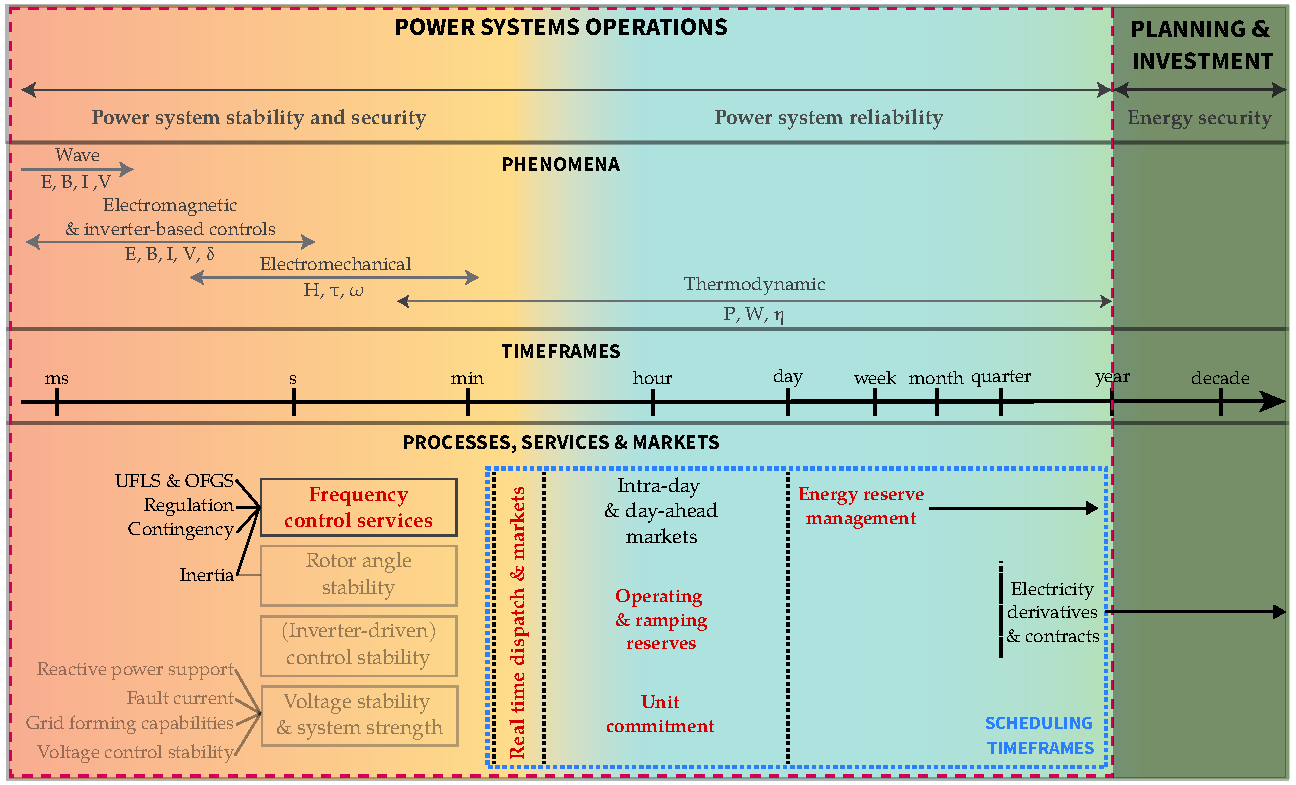
\includegraphics[width=1.3\textwidth,height=\textheight]{source/figures/power_system_timeframes.pdf}
\caption[High-level overview of power system concepts, phenomena and
processes, services and markets relevant within operational
timeframes]{A high-level overview of power system concepts, phenomena
and the processes, services and markets relevant within operational
timeframes (bounded by the red dashed box). All non-faded text in the
bottom section indicates a process, service and/or market
(i.e.~operational practice) related to active power balancing. All bold
red text in the bottom section indicates a process, service and/or
market related to active power balancing that is discussed in detail in
this thesis. Processes, services and markets bounded by the blue dashed
box occur within scheduling timeframes. Phenomena and stability
categories, and their timeframes of relevance, are based on those
discussed in Machowski et al.
(\protect\hyperlink{ref-machowskiPowerSystemDynamics2020}{2020}),
Hatziargyriou et al.
(\protect\hyperlink{ref-hatziargyriouDefinitionClassificationPower2021}{2021})
and Matevosyan et al.
(\protect\hyperlink{ref-matevosyanFutureInverterBasedResources2021}{2021}).
The figure concept and layout was inspired by a similar figure presented
in Wilson
(\protect\hyperlink{ref-wilsonIntroductoryPresentation20202020}{2020}).}\label{fig:power_system_timeframes}
}
\end{figure}

\elandscape

\hypertarget{phenomena-in-operational-timeframes}{%
\subsection{Phenomena in operational
timeframes}\label{phenomena-in-operational-timeframes}}

A knowledge of physical power system phenomena and the timescales in
which they occur is an important prerequisite to achieving good outcomes
when designing operational practices for power systems. As shown in
Figure~\ref{fig:power_system_timeframes}, power system operations is
concerned with three phenomena that dominate on timescales ranging from
a few milliseconds to several months
(\protect\hyperlink{ref-hatziargyriouDefinitionClassificationPower2021}{Hatziargyriou
et al., 2021};
\protect\hyperlink{ref-machowskiPowerSystemDynamics2020}{Machowski et
al., 2020}):

\begin{enumerate}
\def\labelenumi{\arabic{enumi}.}
\item
  \emph{Electromagnetic} phenomena arise from the coupling of electrical
  and magnetic fields within \textbf{synchronous machines} (generators
  and motors that rotate at a speed proportional to AC frequency) and
  between power system resources. They occur on the timescale of
  milliseconds to seconds. IBR controls also operate in this timeframe.
\item
  \emph{Electromechanical} phenomena are slower (seconds to minutes )
  and arise as a result of electromagnetic fields interacting with
  rotating masses and mechanical forces. These typically occur in
  generators and motors.
\item
  \emph{Thermodynamic} phenomena are slower still. They encompass
  chemical fuel conversion and heat transfer processes in boilers. These
  phenomena occur over seconds to minutes to hours. The dynamics of the
  primary energy sources for hydroelectricity and VRE are also studied
  across these timescales
  (\protect\hyperlink{ref-keeratimahatAnalysisShorttermOperational2021}{Keeratimahat
  et al., 2021}).
\end{enumerate}

\hypertarget{sec:lit_review-balancing}{%
\subsection{Active power balancing}\label{sec:lit_review-balancing}}

\textbf{Active power balancing} can be described in simple terms using
the law of conservation of energy: the energy supplied into a network
node through primary energy conversion, energy storage or transmission
is equal to the sum of the energy dissipated, stored, consumed and
transmitted away from the same network node at each and every moment. A
more practical definition that encompasses the key concerns of power
system engineers is that active power balancing requires
\emph{real-time} control of generation and loads to balance active power
supply and demand \emph{across the power system}:

\begin{itemize}
\tightlist
\item
  \emph{Real-time} (i.e.~moment-to-moment) control of supply and demand
  is required because it is still uneconomical in many jurisdictions to
  store electricity at scale despite grid-scale storage cost reductions
  (\protect\hyperlink{ref-internationalenergyagencyGridScaleStorage2022}{International
  Energy Agency, 2022}). In other words, many power systems have small
  balancing buffers and thus require real-time balancing.
\item
  Whilst electricity can be transported close to the speed to light
  across a synchronous area, some degree of balancing coordination
  \emph{across the power system} is required because of transmission
  losses and constraints on network flows imposed by line thermal
  limits, stability requirements and Kirchoff's circuit laws
  (\protect\hyperlink{ref-hirthWhyWindNot2016a}{Hirth et al., 2016};
  \protect\hyperlink{ref-kirschenFundamentalsPowerSystem2004}{Kirschen
  and Strbac, 2004}). A whole-of-system approach is also necessary
  because active power imbalances in network sub-regions can have
  system-wide consequences (see
  Section~\ref{sec:lit_review-balancing_need}).
\end{itemize}

\hypertarget{sec:lit_review-balancing_need}{%
\subsubsection{Why is balancing
required?}\label{sec:lit_review-balancing_need}}

Unlike many other commodity transportation networks, an active power
supply-demand imbalance can lead to deviations in technical parameters
-- voltage and AC frequency -- that not only have the potential to
damage equipment connected to the power system, but also to trigger a
system collapse (see
Section~\ref{sec:lit_review-balancing_need-consequences})
(\protect\hyperlink{ref-borensteinEconomicsElectricityReliability2023}{Borenstein
et al., 2023}).

\hypertarget{sec:lit_review-balancing_need-frequency}{%
\paragraph{The relationship between active power balance and AC
frequency}\label{sec:lit_review-balancing_need-frequency}}

The presence of synchronous machines in most power systems means that
system active power balance is closely tied to the system's AC
frequency. During stable operation, synchronous machines rotate at a
\textbf{synchronous speed} (\(N_s\)) that is proportional to the power
system frequency (\(f\)) (Equation~\ref{eq:synch_speed})
(\protect\hyperlink{ref-chapmanElectricMachineryFundamentals2011}{Chapman,
2011}):

\begin{equation}\protect\hypertarget{eq:synch_speed}{}{N_s = \frac{120f}{P}}\label{eq:synch_speed}\end{equation}
where \(N_s\) is the synchronous speed in revolutions per minute, \(P\)
is the number of (rotor) magnetic poles and \(f\) is the electrical
frequency in Hertz (Hz).

Equation~\ref{eq:synch_speed} describes an important characteristic of
synchronous machines during stable operation, but the link between
active power balance and power system frequency requires examining
synchronous machine \emph{dynamics}. As shown in
Figure~\ref{fig:synch_torques}, the interaction between the magnetic
fields of the rotor and stator of a synchronous generator
(e.g.~coal-fired, gas-fired and hydro generation) produces an
electromagnetic torque (\(T_e\)) on the rotor that opposes the
mechanical torque (\(T_m\)) supplied by a prime mover (e.g.~steam
turbine). Equation~\ref{eq:swing}, which is a variation of what is known
as the swing equation, is an energy balance across the synchronous
generator. It shows that if there is a transient increase in the
electrical load of the power system (equivalent to an increase in
\(P_e\) and thus \(T_e\)), the rotor of a synchronous generator will
begin to decelerate as its stored kinetic energy is converted to
electrical energy
(\protect\hyperlink{ref-elgerdElectricEnergySystems1971}{Elgerd, 1971};
\protect\hyperlink{ref-graingerPowerSystemAnalysis1994}{Grainger,
1994}).

\begin{equation}\protect\hypertarget{eq:swing}{}{J\omega_{sm}\frac{d\omega_{sm}}{dt} = P_m - P_e}\label{eq:swing}\end{equation}
where \(\omega_{sm}\) is the synchronous machine rotor shaft velocity,
\(J\) is moment of inertia of the rotor, \(P_m\) is mechanical power,
\(T_m\) is mechanical torque, \(P_e\) is electrical power and \(T_e\) is
electromagnetic torque.

\begin{figure}
\hypertarget{fig:synch_torques}{%
\centering
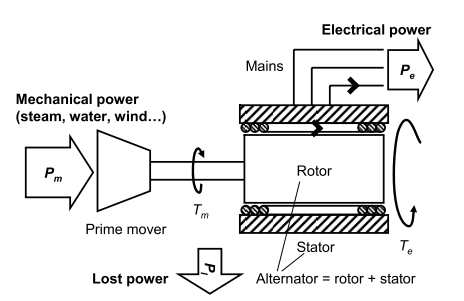
\includegraphics[width=0.6\textwidth,height=\textheight]{source/figures/swing.png}
\caption[Mechanical and electromagnetic torques on a synchronous
generator]{Mechanical power applied to the prime mover results in a
mechanical torque \(T_m\) on the rotor of a synchronous generator. This
is opposed by an electromagnetic torque \(T_e\) that is produced from
the interaction between the rotor and stator magnetic fields. Source:
Rebours
(\protect\hyperlink{ref-reboursComprehensiveAssessmentMarkets2009}{2009})}\label{fig:synch_torques}
}
\end{figure}

The relationship between the active power imbalance in a power system
(\(P_{gen}-P_{load}\)) and AC frequency is obtained by extending the
swing equation from a single synchronous generator to all synchronous
generators in a synchronous area (Equation~\ref{eq:swing_area}).
Equation~\ref{eq:swing_area} shows that the rate of change of frequency
(RoCoF) is proportional to the active power imbalance and inversely
proportional to the system's inertia constant, \(H\). This form of the
swing equation only models the \textbf{inertial response} of synchronous
generators; that is, it does not include the load damping response
offered by (frequency-dependent) induction motor loads. The generation
inertia constant is often used as a proxy for the system inertia
constant since the high speed and mass of generator rotors mean that
they store significant quantities of kinetic energy
(\protect\hyperlink{ref-denholmInertiaPowerGrid2020}{Denholm et al.,
2020}; \protect\hyperlink{ref-ulbigImpactLowRotational2014}{Ulbig et
al., 2014}).

\begin{equation}\protect\hypertarget{eq:swing_area}{}{\frac{2H}{f}\frac{df}{dt} = \frac{P_{gen}-P_{load}}{S_{g, total}}}\label{eq:swing_area}\end{equation}
where \(H\) is the inertia constant of the synchronous area
(\(H=\sum_{g} H_g\), where \(H_g = \frac{J_g(2\pi f)^2}{2S_g}\)), \(f\)
is the AC frequency, \(\frac{df}{dt}\) is the rate of change of
frequency or RoCoF, \(S_{g,total}\) is the total apparent power of
synchronous generators, and \(P_{gen}\) and \(P_{load}\) are the power
system's total active power supply and active power demand (including
losses), respectively.

Equation~\ref{eq:swing_area} shows that a power system's AC frequency is
an indicator of active power balance
(\protect\hyperlink{ref-bagginiHandbookPowerQuality2008}{Baggini,
2008}). Insufficient generation will lead to a \emph{decrease} in system
frequency (i.e.~negative RoCoF) and oversupply will lead to an
\emph{increase} in system frequency (i.e.~positive RoCoF).

\hypertarget{sec:lit_review-balancing_need-consequences}{%
\paragraph{The consequences of frequency
deviations}\label{sec:lit_review-balancing_need-consequences}}

Serious power system frequency deviations away from the nominal value
can have harmful effects. Synchronous machines may experience
equipment-damaging vibrations
(\protect\hyperlink{ref-ulbigImpactLowRotational2014}{Ulbig et al.,
2014}), and both synchronous machines and transformers can overheat and
fail if they operate outside their rated voltage-frequency limits
(\protect\hyperlink{ref-kirbyFrequencyControlConcerns2002}{Kirby et al.,
2002}). Synchronous machines are also vulnerable to damage from high
RoCoFs due to pole slipping
(\protect\hyperlink{ref-dgaconsultingInternationalReviewFrequency2016}{DGA
Consulting, 2016}). For these reasons, frequency-sensitive relays are
often used to protect power system resources from frequency excursions.

However, these same equipment protection measures can also trigger the
complete collapse of the power system. Should the disconnection of a
resource following a relay trip exacerbate an existing active power
imbalance, the system frequency may deviate further and result in
further disconnections. Situations such as these are known as
\textbf{cascading failures} and can lead to the collapse of the entire
power system. As such, SOs often employ emergency frequency control
schemes to arrest imbalances by tripping loads in the event of
under-frequency (under-frequency load shedding or \textbf{UFLS}) or
generation in the event of over-frequency (over-frequency generation
shedding or \textbf{OFGS})
(\protect\hyperlink{ref-australianenergymarketoperatorEnduringPrimaryFrequency2021}{Australian
Energy Market Operator, 2021a};
\protect\hyperlink{ref-hartmannEffectsDecreasingSynchronous2019}{Hartmann
et al., 2019}). The activation of these schemes is undesirable,
particularly since UFLS can lead to power system reliability standards
being breached.

\hypertarget{sec:lit_review-balancing_threats}{%
\subsubsection{Threats to active power
balance}\label{sec:lit_review-balancing_threats}}

Threats to active power balance can be broadly categorised as either
power system \textbf{variability} or power system \textbf{uncertainty}.

\hypertarget{power-system-variability}{%
\paragraph{Power system variability}\label{power-system-variability}}

Power system variability refers to \emph{expected} or forecasted changes
to active power supply and/or demand. Sources of variability include
fluctuations in load, oscillatory active power output from synchronous
generators and VRE generation \textbf{ramping} (i.e.~a sustained
increase or decrease in active power output). VRE ramping includes
changes in solar PV generation during sunrise or sunset and in wind
generation with wind speed variations
(\protect\hyperlink{ref-australianenergymarketoperatorRenewableIntegrationStudy2020}{Australian
Energy Market Operator, 2020a};
\protect\hyperlink{ref-bloomItIndisputableFive2017}{Bloom et al., 2017};
\protect\hyperlink{ref-elaOperatingReservesVariable2011}{Ela et al.,
2011}).

\hypertarget{power-system-uncertainty}{%
\paragraph{Power system uncertainty}\label{power-system-uncertainty}}

Power system uncertainty refers to \emph{unexpected} changes to active
power supply and/or demand. Source of uncertainty include demand and VRE
generation forecast errors, and singular or widespread outage events
triggered by the weather or unexpected system responses and
interactions.
(\protect\hyperlink{ref-australianenergymarketoperatorRenewableIntegrationStudy2020}{Australian
Energy Market Operator, 2020a};
\protect\hyperlink{ref-egglestonSecurityResilienceTechnical2021}{Eggleston
et al., 2021};
\protect\hyperlink{ref-elaOperatingReservesVariable2011}{Ela et al.,
2011}).

\hypertarget{sec:lit_review-operational_paradigms}{%
\subsection{Operational
paradigms}\label{sec:lit_review-operational_paradigms}}

Though governance and operational arrangements vary from jurisdiction to
jurisdiction, the powers, responsibilities and degree of ring-fencing
imposed upon the SO are largely dictated by the operational paradigm of
the control area
(\protect\hyperlink{ref-chawlaGlobalTrendsElectricity2013}{Chawla and
Pollitt, 2013}). Below, I discuss the two possible operational
paradigms: where the SO is a \textbf{vertically-integrated utility}, and
where the SO is, at the very least, responsible for operating a
transmission system that forms the physical basis of a \textbf{wholesale
electricity market}. In both cases, it is the SO that is ultimately
responsible for ensuring that the transmission network in their control
area is operated in a secure and reliable manner
(\protect\hyperlink{ref-roquesMarketDesignGeneration2008}{Roques,
2008}).

\hypertarget{vertically-integrated-utility}{%
\subsubsection{Vertically-integrated
utility}\label{vertically-integrated-utility}}

Under this paradigm, a single company (either state-owned or
privately-owned but regulated) owns, operates and invests in generation,
transmission and distribution infrastructure, as well as being
responsible for the retail of electricity to the end-user. This was the
sole operational paradigm for much of the 20\textsuperscript{th}
century. Having a single owner and operator of power system resources
reduces complexity and transaction costs, and enables economies of scale
in both asset investment (particularly generation infrastructure) and
operation
(\protect\hyperlink{ref-sioshansiElectricityMarketReform2006}{Sioshansi,
2006}). The benefits from economies of scale are material where
industrialisation and/or electrification are driving sustained load
growth. This was the case in advanced economies in the
20\textsuperscript{th} century and is still the case in many emerging
economies
(\protect\hyperlink{ref-hoganElectricityMarketStructure2008}{Hogan,
2008};
\protect\hyperlink{ref-roquesAdaptingElectricityMarkets2017}{Roques and
Finon, 2017}).

\hypertarget{wholesale-electricity-markets}{%
\subsubsection{Wholesale electricity
markets}\label{wholesale-electricity-markets}}

Beginning in the late 1980s, some jurisdictions opted to
\textbf{restructure} their electricity sector. To varying degrees across
different jurisdictions, the impetuses for restructuring included
advancements in small low-upfront cost gas turbine technologies, the
promise of consumer choice, perceptions that vertically-integrated
utilities were inefficient and politicised, and a political zeitgeist
prevalent at the time that pursued economic efficiency through
privatisation and competition
(\protect\hyperlink{ref-chesterEnergyProblemRepresentation2019}{Chester
and Elliot, 2019};
\protect\hyperlink{ref-macgillElectricityIndustryReform2013}{MacGill and
Healy, 2013};
\protect\hyperlink{ref-simshauserLessonsAustraliaNational2019}{Simshauser,
2019};
\protect\hyperlink{ref-sioshansiElectricityMarketReform2006}{Sioshansi,
2006}). Two features common to electricity industry restructuring
processes were the unbundling of vertically-integrated utilities and the
introduction of competition for wholesale supply (and in some cases,
demand) via an \textbf{electricity market} -- an auction-based mechanism
for the sale and/or purchase of electrical energy.

\hypertarget{unbundling}{%
\paragraph{Unbundling}\label{unbundling}}

In most cases, the unbundling of a vertically-integrated utility divided
generation ownership and barred the SO from owning generation assets. In
some jurisdictions, SOs retained ownership of the transmission network
(e.g.~Transmission System Operators, or TSOs, in many European control
areas) whereas others made their SOs ``independent'' by relieving them
of any asset ownership (e.g.~Independent System Operators in North
American control areas). Some SOs, such as those in North America and
the Australian NEM, were also given market operation responsibilities
(\protect\hyperlink{ref-chawlaGlobalTrendsElectricity2013}{Chawla and
Pollitt, 2013}).

\hypertarget{market-models}{%
\paragraph{Market models}\label{market-models}}

The design and implementation of wholesale electricity markets differs
across jurisdictions that undertook electricity industry restructuring.
Despite these differences, electricity markets worldwide can broadly be
categorised into two markets models\footnote{My descriptions of central
  and self-dispatch electricity markets differ slightly to those of
  Ahlqvist et al.
  (\protect\hyperlink{ref-ahlqvistSurveyComparingCentralized2022}{2022}),
  who focus on the level of centralisation in day-ahead timeframes. They
  categorise the Australian NEM as a decentralised market as
  participants manage unit commitment. However, the SO still produces
  resource-specific production and consumption targets through a central
  dispatch process that also clears the real-time market. As such, I
  categorise the NEM as a semi-centralised market (refer to
  Section~\ref{sec:info-context-nem}).} that are distinguished by the
degree of centralisation in system and market operations
(\protect\hyperlink{ref-ahlqvistSurveyComparingCentralized2022}{Ahlqvist
et al., 2022};
\protect\hyperlink{ref-barrosoClassificationElectricityMarket2005}{Barroso
et al., 2005};
\protect\hyperlink{ref-cramtonElectricityMarketDesign2017}{Cramton,
2017}):

\begin{enumerate}
\def\labelenumi{\arabic{enumi}.}
\item
  \textbf{Central dispatch} markets, where decisions regarding dispatch
  and, in some cases, unit commitment (see
  Section~\ref{sec:lit_review-balancing_practices-scheduling}) are made
  by the SO. System and market operations are often \textbf{integrated}
  (i.e.~the SO is also the market operator) through a \textbf{mandatory
  power pool} in which supply offers are aggregated and cleared against
  a demand forecast (one-sided pool), or against an aggregated demand
  curve constructed from potential buyers (two-sided pool)
  (\protect\hyperlink{ref-barrosoClassificationElectricityMarket2005}{Barroso
  et al., 2005}). In these markets, locational prices for energy and
  \textbf{ancillary services} (services procured to maintain security
  and reliability) are produced by SO-run centralised optimisation
  processes that consider the physical constraints of the transmission
  system. This market model has been adopted in Independent System
  Operator/Regional Transmission Operator (ISO/RTO) markets in North
  America (refer to Section~\ref{sec:fcs-NA} for more detail). As I
  discuss further in Section~\ref{sec:info-context-nem}, the Australian
  NEM's design is predominantly based on this model though it does
  incorporate some features of more decentralised markets.
\item
  Decentralised or \textbf{self-dispatch} markets, where decisions
  regarding dispatch and unit commitment are made by market
  participants, and in which system and market operations are more
  decoupled. These types of markets facilitate trade through bilateral
  contracts between suppliers and buyers. Whilst scheduling and dispatch
  is managed by market participants, they are required to submit
  intended schedules to the SO ahead of delivery (often during the day
  before delivery). The SO is responsible for taking redispatch actions
  to ensure that transmission constraints are not violated, and for
  determining the requirement for and procuring balancing services
  (another name for frequency control services, which I discuss in
  greater detail in
  Section~\ref{sec:lit_review-balancing_practices-fcs}) that maintain
  system balance following market gate closure. As outlined in
  Section~\ref{sec:fcs-EU}, this is the dominant market model in Europe.
\end{enumerate}

Figure~\ref{fig:market_models} shows the primary and secondary
commercial arrangements in each of these market models. A mandatory
power pool is the primary exchange mechanism in central dispatch
markets, whereas self-dispatch markets are designed to facilitate
exchange through bilateral contracts. However, both exchange mechanisms
are present in each market model. Bilateral contracts (in the form of
derivatives) are often used as hedging instruments in central dispatch
markets, and several self-dispatch markets, such as those in Europe,
have associated voluntary power exchanges that are essentially power
pools
(\protect\hyperlink{ref-barrosoClassificationElectricityMarket2005}{Barroso
et al., 2005}).

\begin{figure}
\hypertarget{fig:market_models}{%
\centering
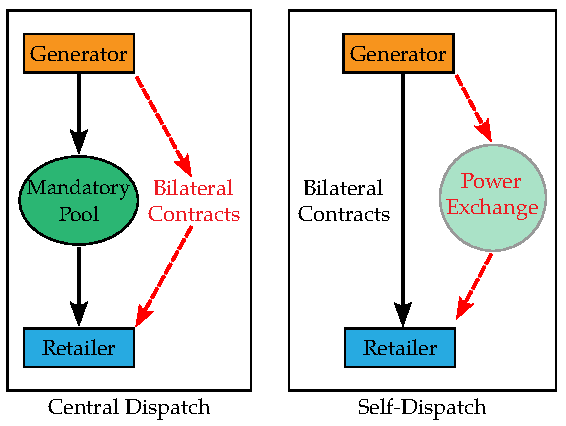
\includegraphics{source/figures/market_models.pdf}
\caption[Primary and secondary commercial arrangements in central and
self-dispatch electricity markets]{Primary and secondary commercial
arrangements in central and self-dispatch electricity markets.
Reproduced from Barroso et al.
(\protect\hyperlink{ref-barrosoClassificationElectricityMarket2005}{2005}).}\label{fig:market_models}
}
\end{figure}

\hypertarget{sec:lit_review-operational_paradigms-markets-platforms}{%
\paragraph{Market
platforms}\label{sec:lit_review-operational_paradigms-markets-platforms}}

Power system resource inflexibilities and the desire for physical and
financial risk management mechanisms in operational timeframes have
driven policy-makers in many jurisdictions to design and implement
electricity markets with multiple market \textbf{platforms}
(\protect\hyperlink{ref-energysecurityboardSystemServicesAhead2020}{Energy
Security Board, 2020a};
\protect\hyperlink{ref-isemongerBenefitsRisksVirtual2006}{Isemonger,
2006}). Platforms are formal sub-markets for energy (and sometimes
ancillary services) that are cleared ahead of the delivery of
electricity and/or ancillary services. The number of platforms
implemented in a particular market is often related to its market model.
Self-dispatch markets can maximise trade and better facilitate market
participants balancing their positions by implementing multiple market
platforms (typically day-ahead and several intra-day, see
Section~\ref{sec:fcs-EU}), whereas the number of platforms in central
dispatch markets (typically real-time and in most cases, day-ahead) is
limited by the computational complexity of the optimisation algorithm(s)
used by the SO to clear each market platform (see
Section~\ref{sec:fcs-NA} and Section~\ref{sec:fcs-nem})
(\protect\hyperlink{ref-ahlqvistCentralSelfDispatchElectricity2018}{Ahlqvist
et al., 2018}).

\hypertarget{sec:lit_review-balancing_practices}{%
\section{Balancing practices in operational
timeframes}\label{sec:lit_review-balancing_practices}}

SOs employ \textbf{balancing practices} in operational timeframes
(including the non-faded processes, services and markets shown in
Figure~\ref{fig:power_system_timeframes}) to obtain \textbf{balancing
flexibility}. Balancing flexibility is procured either to address
variability directly, or as optionality to manage uncertainty
(\protect\hyperlink{ref-heggartyQuantifyingPowerSystem2020}{Heggarty et
al., 2020},
\protect\hyperlink{ref-heggartyQuantifyingPowerSystem2020}{2020};
\protect\hyperlink{ref-papaefthymiou100RenewableEnergy2016}{Papaefthymiou
and Dragoon, 2016}). Though the particularities of these practices vary
between jurisdictions, they are almost always organised in a
hierarchical and sequential fashion to ensure that active power supply
and demand are continuously balanced across different timeframes.
Furthermore, in jurisdictions that have restructured their electricity
industries, balancing practices that were previously administered by a
vertically-integrated utility have been adapted into or integrated with
market-based mechanisms.

In the subsections that follow, I describe balancing practices in the
order of the timescales in which they are relevant.

\hypertarget{sec:lit_review-balancing_practices-fcs}{%
\subsection{Frequency control
services}\label{sec:lit_review-balancing_practices-fcs}}

\textbf{Frequency control services} (leftmost section of the processes,
services and markets shown in Figure~\ref{fig:power_system_timeframes})
are ancillary services used by the SO to contain AC frequency within as
narrow a band as possible during normal operation and following
\textbf{contingency events} (sudden disturbances)
(\protect\hyperlink{ref-etoFrequencyControlRequirements2018}{Eto et al.,
2018}). With the exception of inertial response from synchronous
machines
(Section~\ref{sec:lit_review-balancing_practices-inertial_response}),
these services are provided by power system resources with 1) the
appropriate control system configurations and 2) capacity flexibility in
the form of \textbf{headroom} (the ability to increase active power
output) for responding to an under-frequency event and/or
\textbf{footroom} (the ability to decrease active power output) for
responding to an over-frequency event
(\protect\hyperlink{ref-etoUseFrequencyResponse2010}{Eto et al., 2010}).
Vertically-integrated utilities schedule their own resources to provide
frequency control services, whereas SOs in restructured electricity
industries typically procure frequency control services through
regulatory and market-based mechanisms (see
Section~\ref{sec:fcs-context-procurement}).

As shown in Figure~\ref{fig:freq_control} and discussed further in
Section~\ref{sec:fcs}, the conventional frequency control services
described below differ based on their purpose, response time and
activation and control methods.

\begin{figure}
\hypertarget{fig:freq_control}{%
\centering
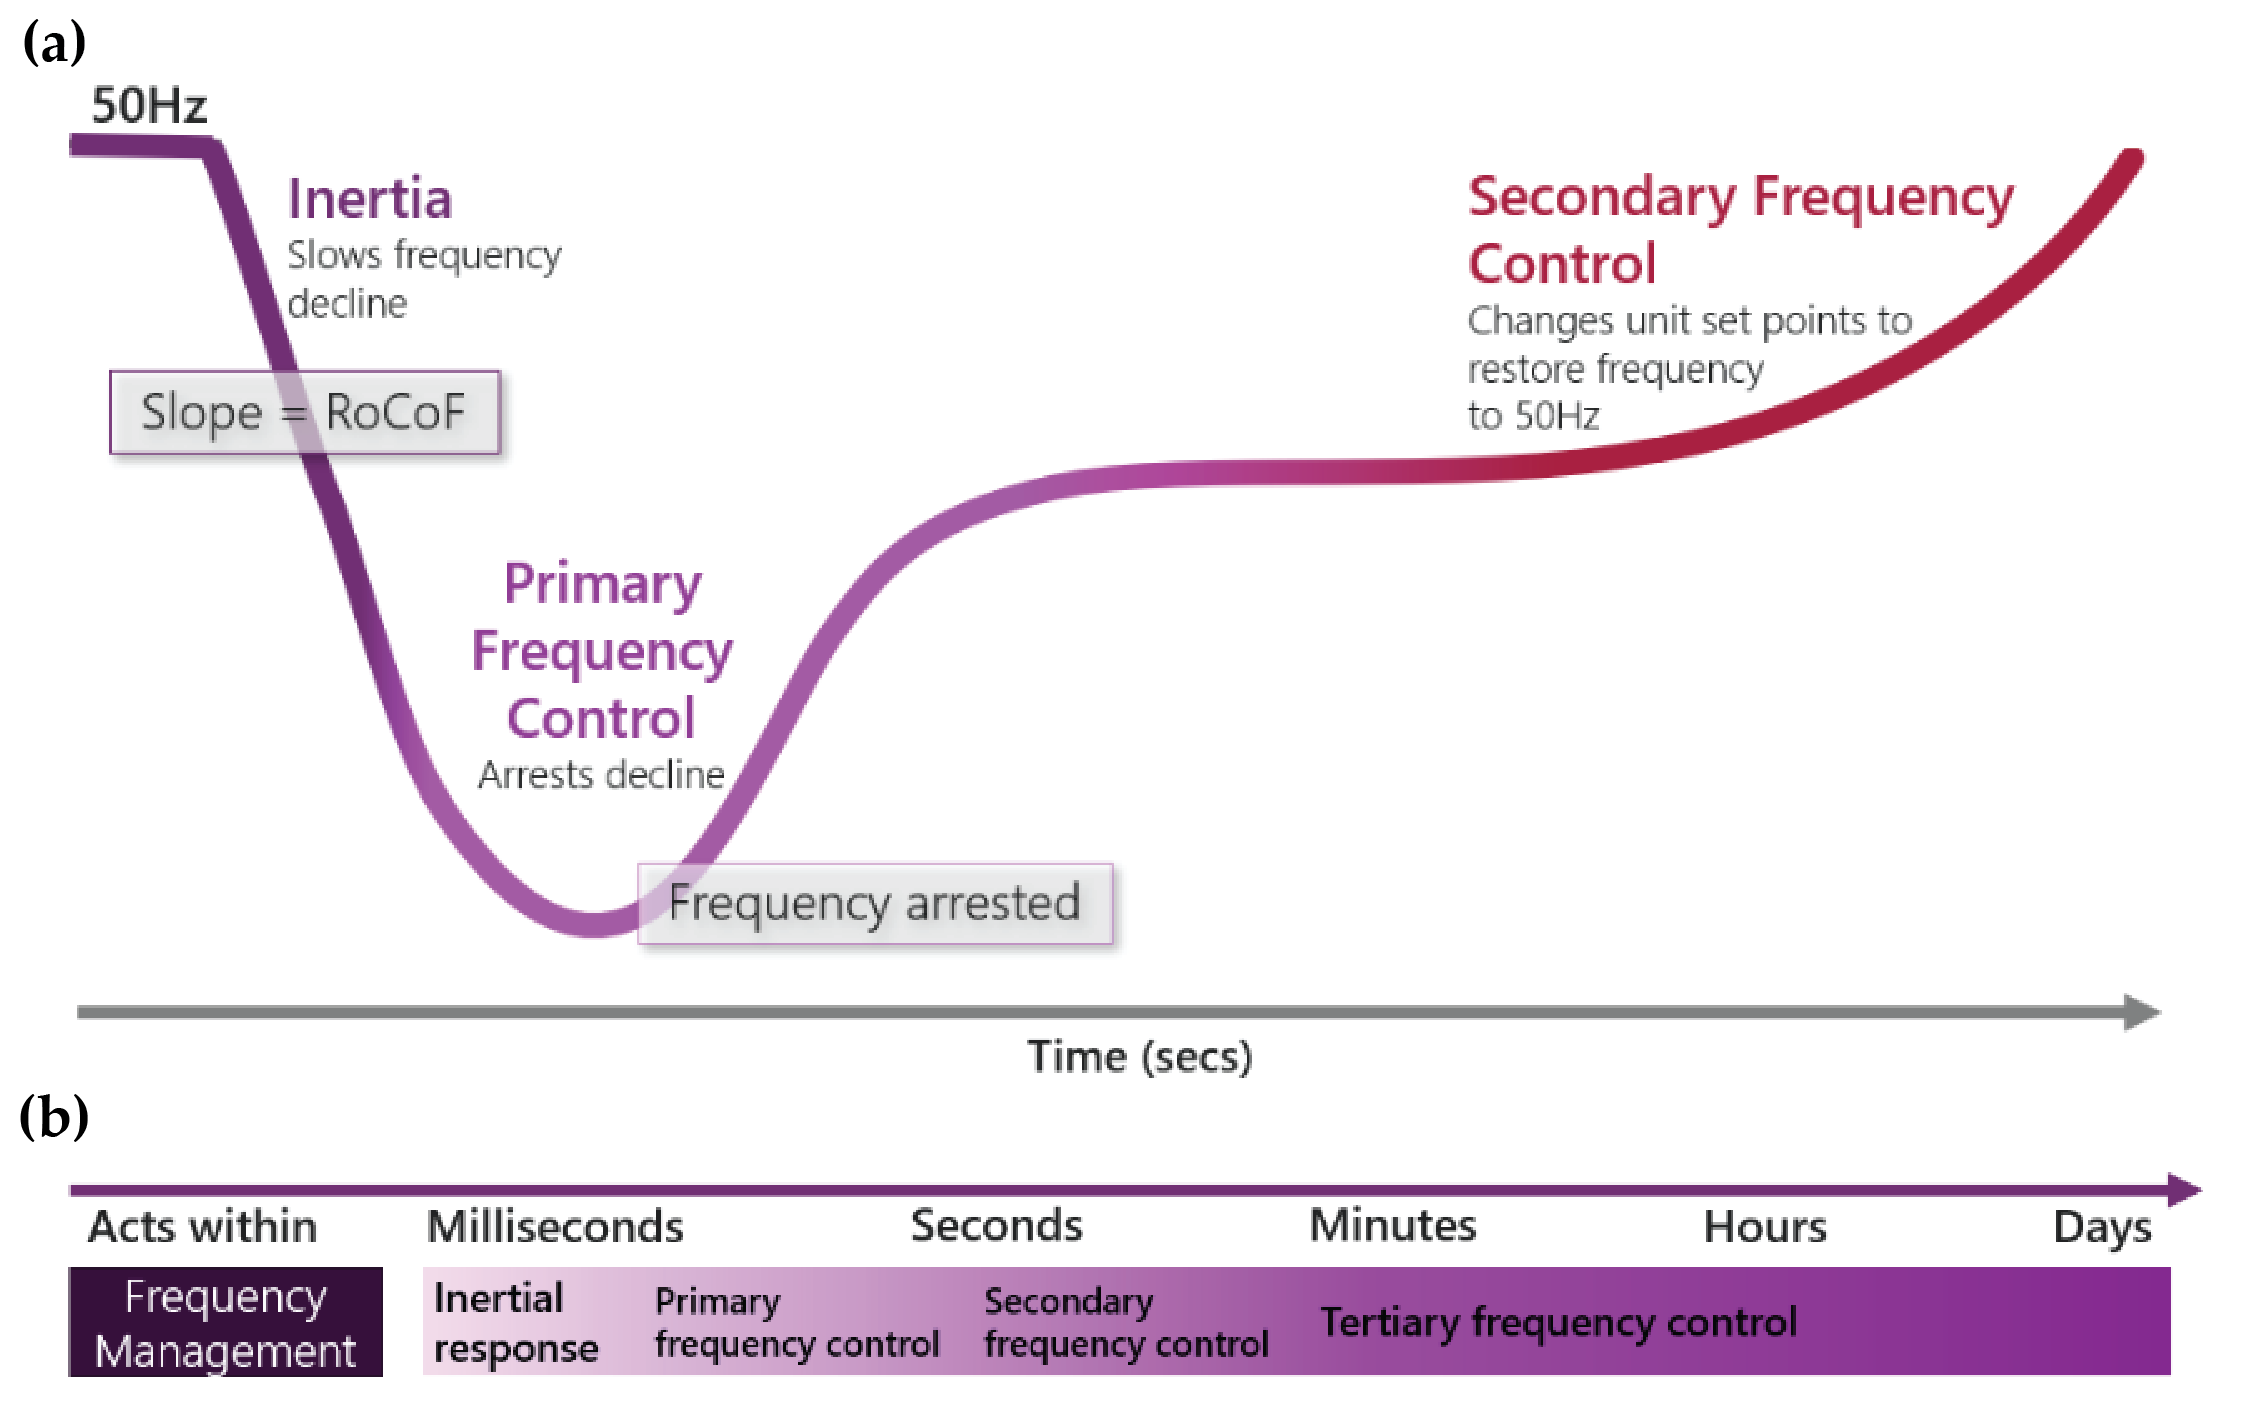
\includegraphics{source/figures/freq_control_timeframes.png}
\caption[Sequence and timescales of typical frequency control
services]{(a) A trace of power system frequency with corresponding
frequency control services following a loss-of-generation contingency
event. (b) The timescales over which the various frequency control
services are provided. Source: Australian Energy Market Operator
(\protect\hyperlink{ref-australianenergymarketoperatorPowerSystemRequirements2020}{2020b})}\label{fig:freq_control}
}
\end{figure}

\hypertarget{sec:lit_review-balancing_practices-inertial_response}{%
\subsubsection{Inertial
response}\label{sec:lit_review-balancing_practices-inertial_response}}

As discussed in Section~\ref{sec:lit_review-balancing_need-frequency},
synchronous machines have an \emph{inherent} inertial response to AC
frequency deviations that must be considered in the frequency control
strategy of a power system. For a given active power imbalance, the
inertia constant of the synchronous area (\(H\) in
Equation~\ref{eq:swing_area}) determines the magnitude of the initial
RoCoF following an imbalance event and the speed at which the power
system can be returned to its nominal frequency
(\protect\hyperlink{ref-tielensRelevanceInertiaPower2016}{Tielens and
Van Hertem, 2016};
\protect\hyperlink{ref-ulbigImpactLowRotational2014}{Ulbig et al.,
2014}).

\hypertarget{fast-frequency-response}{%
\subsubsection{Fast frequency response}\label{fast-frequency-response}}

IBRs and loads on frequency-responsive relays can provide what is
typically known as fast frequency response (FFR). The most
well-discussed use-case for FFR is mitigating high RoCoFs through a
response delivered within a matter of milliseconds to a few seconds
following a contingency event
(\protect\hyperlink{ref-australianenergymarketoperatorFastFrequencyResponse2017}{Australian
Energy Market Operator, 2017a};
\protect\hyperlink{ref-millerTechnologyCapabilitiesFast2017}{Miller et
al., 2017b}). As I also touch upon in
Section~\ref{sec:fcs-ibr-challenges}, the term FFR has been used rather
loosely to date to refer to three distinct control configurations:

\begin{enumerate}
\def\labelenumi{\arabic{enumi}.}
\tightlist
\item
  An \emph{inherent} response delivered by IBRs that, though lacking a
  spinning mass, resembles the inertial response of synchronous machines
  (sometimes referred to as virtual inertia)
  (\protect\hyperlink{ref-linResearchRoadmapGridForming2020}{Lin et al.,
  2020});
\item
  A \emph{controlled} response delivered by wind generation in which
  kinetic energy is extracted from a wind turbine rotor to rapidly
  inject active power into the system (sometimes referred to as
  synthetic inertia or inertia-based FFR)
  (\protect\hyperlink{ref-erikssonSyntheticInertiaFast2018}{Eriksson et
  al., 2018};
  \protect\hyperlink{ref-nercinverter-basedresourceperformancetaskforceFastFrequencyResponse2020}{NERC
  Inverter-Based Resource Performance Task Force, 2020});
\item
  A \emph{controlled and sustained} response delivered by IBRs and
  frequency-responsive loads that is more or less a faster version of
  primary frequency response
  (Section~\ref{sec:lit_review-balancing_practices-pfr})
  (\protect\hyperlink{ref-dreidyInertiaResponseFrequency2017}{Dreidy et
  al., 2017};
  \protect\hyperlink{ref-fernandez-guillamonPowerSystemsHigh2019}{Fernández-Guillamón
  et al., 2019};
  \protect\hyperlink{ref-nercinverter-basedresourceperformancetaskforceFastFrequencyResponse2020}{NERC
  Inverter-Based Resource Performance Task Force, 2020}).
\end{enumerate}

\hypertarget{sec:lit_review-balancing_practices-pfr}{%
\subsubsection{Primary frequency
response}\label{sec:lit_review-balancing_practices-pfr}}

The aim of primary frequency response (PFR) is to arrest a frequency
deviation. PFR is implemented in resource-level control systems such
that each enabled resource provides a response to locally-measured
frequency deviations that exceed a certain control dead-band
(\protect\hyperlink{ref-elaAlternativeApproachesIncentivizing2012}{Ela
et al., 2012b};
\protect\hyperlink{ref-wangReviewAGCImplementation2003}{Wang and
Hiskens, 2003}). For generators, this is achieved through \textbf{droop
control}, in which a synchronous speed deviation produces a change in
the active power output of a generator according to its droop
characteristic (Figure~\ref{fig:droop}, e.g.~from \(A\) to \(B\) along
\(L_0\)). Droop control is implemented in the turbine governors of
synchronous generators and the inverter control systems of IBRs
(\protect\hyperlink{ref-fernandez-guillamonPowerSystemsHigh2019}{Fernández-Guillamón
et al., 2019};
\protect\hyperlink{ref-linResearchRoadmapGridForming2020}{Lin et al.,
2020}). Provided there is a sufficient amount of PFR reserve to arrest
the system frequency, the frequency \textbf{zenith}/\textbf{nadir}
(maximum/minimum system frequency following an active power imbalance
event) is determined by the size of the initial imbalance, the inertia
constant of the synchronous area, the droop characteristics of power
system resources and the speed of PFR
(\protect\hyperlink{ref-nercinverter-basedresourceperformancetaskforceFastFrequencyResponse2020}{NERC
Inverter-Based Resource Performance Task Force, 2020}). PFR should
ideally be sustained until secondary frequency control can take over
(i.e.~several to tens of seconds)
(\protect\hyperlink{ref-etoUseFrequencyResponse2010}{Eto et al., 2010};
\protect\hyperlink{ref-etoFrequencyControlRequirements2018}{Eto et al.,
2018}; \protect\hyperlink{ref-undrillNotesFrequencyControl2019}{Undrill,
2019},
\protect\hyperlink{ref-undrillPrimaryFrequencyResponse2018}{2018}).

\hypertarget{secondary-frequency-control}{%
\subsubsection{Secondary frequency
control}\label{secondary-frequency-control}}

Secondary frequency response (SFR) is designed to relieve fast-acting
PFR. SFR is implemented in resource-level load controllers, which can
(\protect\hyperlink{ref-etoFrequencyControlRequirements2018}{Eto et al.,
2018}; \protect\hyperlink{ref-undrillNotesFrequencyControl2019}{Undrill,
2019}).:

\begin{enumerate}
\def\labelenumi{\arabic{enumi}.}
\tightlist
\item
  Be pre-configured to respond following a frequency deviation through a
  frequency bias setting. This could include sustaining
  already-delivered PFR (as shown in Figure~\ref{fig:droop}); or
\item
  Receive control signals from Automatic Generation Control (AGC), a
  control system used by the SO to coordinate SFR across the control
  area. The AGC's control objective is to minimise Area Control Error
  subject to a tie-line bias and thus return power system frequency to
  its nominal value. Following the calculation of a required response
  that occurs in each cycle (these are typically several seconds apart),
  the AGC then communicates with each enabled resources to provide them
  with active power adjustment targets
  (\protect\hyperlink{ref-machowskiPowerSystemDynamics2020}{Machowski et
  al., 2020}). The service provided by these enabled resources is
  referred to as \textbf{regulation} in many jurisdictions
  (\protect\hyperlink{ref-elaOperatingReservesVariable2011}{Ela et al.,
  2011};
  \protect\hyperlink{ref-hewickerDimensioningControlReserves2020}{Hewicker
  et al., 2020}).
\end{enumerate}

\begin{figure}
\hypertarget{fig:droop}{%
\centering
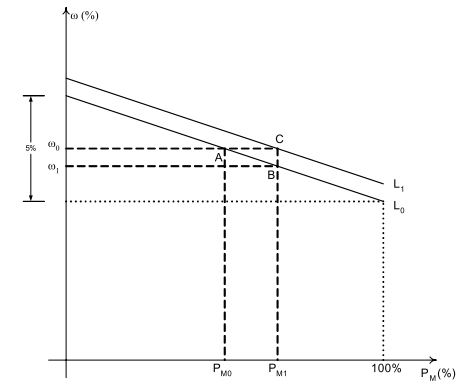
\includegraphics[width=0.75\textwidth,height=\textheight]{source/figures/droop.png}
\caption[An example of secondary frequency response sustaining primary
frequency response]{The behaviour of a synchronous generator providing
PFR and SFR in the absence of other resources with droop control.
\(L_0\) is the initial droop characteristic of the turbine governor. The
generator is initially operating at point A with an active power output
of \(P_{M0}\) and synchronous speed \(\omega_0\). Following an imbalance
event, the system frequency begins to drop as the synchronous generator
provides inertial response. The turbine governor then begins to actuate
and moves the synchronous generator along the droop characteristic. A
new steady-state is reached at point B, where the generator's active
power output is \(P_{M1}\) and the system frequency (and hence the
synchronous speed of the turbine) has decreased to \(\omega_1\). This
constitutes the provision of PFR. Following this, the generator load
controller changes the reference speed setpoint of the governor and thus
shifts the droop characteristic to \(L_1\). This subsequent control
action sustains PFR and returns the system to frequency \(\omega_0\).
This constitutes the provision of SFR. Source: Wang and Hiskens
(\protect\hyperlink{ref-wangReviewAGCImplementation2003}{2003}).}\label{fig:droop}
}
\end{figure}

\hypertarget{tertiary-frequency-control}{%
\subsubsection{Tertiary frequency
control}\label{tertiary-frequency-control}}

In power systems where scheduling processes are infrequently run
(e.g.~vertically-integrated utilities that historically produced hourly
schedules) or in which a ``safety margin'' is desired to address active
power imbalances that endure over multiple scheduling intervals,
tertiary frequency response (TFR) is deployed to relieve PFR and SFR
(\protect\hyperlink{ref-hewickerDimensioningControlReserves2020}{Hewicker
et al., 2020}). Some jurisdictions, such as those operated by the
California and Midcontinent ISOs, have introduced \textbf{ramping
reserves} -- a form of TFR intended to address increased variability and
uncertainty across dispatch intervals (i.e.~several minutes to an hour)
due to growing penetrations of VRE
(\protect\hyperlink{ref-elaElectricityMarketsRenewables2017}{Ela et al.,
2017}; \protect\hyperlink{ref-elaWholesaleElectricityMarket2016}{Ela et
al., 2016}). Other jurisdictions, such as the Australian NEM, rely on
balancing flexibility obtained through frequent scheduling processes
(though the introduction of a TFR service had recently been proposed;
see Section~\ref{sec:reserves-orcontext})
(\protect\hyperlink{ref-australianenergymarketoperatorPowerSystemRequirements2020}{Australian
Energy Market Operator, 2020b};
\protect\hyperlink{ref-rieszFrequencyControlAncillary2015}{Riesz et al.,
2015}).

\hypertarget{sec:lit_review-balancing_practices-scheduling}{%
\subsection{Scheduling}\label{sec:lit_review-balancing_practices-scheduling}}

The purpose of \textbf{scheduling} is to produce efficient (or economic)
generation and consumption schedules for the minutes to days ahead based
on expected power system conditions. In a similar manner to Chow et al.
(\protect\hyperlink{ref-chowElectricityMarketDesign2005}{2005}), I
divide the scheduling problem into three phases: dispatch, unit
commitment and longer-term scheduling.

\hypertarget{dispatch}{%
\subsubsection{Dispatch}\label{dispatch}}

Dispatch involves assigning generation or consumption targets to
already-committed power system resources in real-time (i.e.~several
minutes ahead of delivery). Dispatch is carried out by the monopoly
utility in vertically-integrated electricity industries, the SO in
central dispatch markets and is self-managed by market participants in
self-dispatch markets. In the first two cases, the SO dispatches power
system resources by running a process known as
\textbf{security-constrained economic dispatch}. Security-constrained
economic dispatch seeks to find a minimum cost operating configuration
for committed generation and loads such that a short-term forecast of
non-scheduled demand can be met subject to network constraints and
stability and reliability requirements\footnote{This is a common variant
  of the generic problem description described in
  Section~\ref{sec:lit_review-operations}.}
(\protect\hyperlink{ref-graingerPowerSystemAnalysis1994}{Grainger,
1994}). Some SOs solve this problem for a single interval (e.g.~in the
Australian NEM), whereas others, including the California and
Midcontinent ISOs, solve a multi-period dispatch to procure and, to some
extent, price capabilities to address expected non-scheduled demand
ramps (\protect\hyperlink{ref-elaSchedulingPricingExpected2016}{Ela and
O'Malley, 2016};
\protect\hyperlink{ref-schiroProcurementPricingRamping2017}{Schiro,
2017}). The dispatch solution for each dispatch interval (typically
5--15 minutes long
(\protect\hyperlink{ref-irenaIncreasingTimeGranularity2019}{IRENA,
2019})) consists of generation and consumption setpoints, enablement
quantities for resources providing frequency control services and, in
central dispatch markets that integrate power system and market
operation, real-time market locational marginal prices for energy and
ancillary services
(\protect\hyperlink{ref-cramtonElectricityMarketDesign2017}{Cramton,
2017}). If piecewise linear functions are used by vertically-integrated
utilities to model resource cost curves, or are required by the
real-time market bid format for a market participant's energy offer
curve\footnote{Bid formats may actually require monotonically increasing
  price-quantity pairs, but these can be used to construct piecewise
  linear increasing offer curves.}, the security-constrained economic
dispatch problem can be efficiently solved using linear programming
techniques
(\protect\hyperlink{ref-woodPowerGenerationOperation2014}{Wood et al.,
2014}).

\hypertarget{sec:lit_review-balancing_practices-scheduling-uc}{%
\subsubsection{Unit
commitment}\label{sec:lit_review-balancing_practices-scheduling-uc}}

Thermal and hydroelectric generation, which historically dominated
supply in many power systems, have inflexibility constraints (minimum
load, start-up time, ramping limits and minimum up and down times) and
costs (those attached to resource start-up, shut-down and operation at
minimum load) that require SOs and market participants to make
non-trivial \textbf{unit commitment} decisions (i.e.~whether a resource
should be online or offline). Depending on the resource, these decisions
are made several minutes to hours ahead of power delivery
(\protect\hyperlink{ref-agoraenergiewendeFlexibilityThermalPower2017}{Agora
Energiewende, 2017};
\protect\hyperlink{ref-denholmHowLowCan2018}{Denholm et al., 2018}).
Unit commitment is:

\begin{itemize}
\tightlist
\item
  Managed by vertically-integrated utilities for all resources in
  jurisdictions that have not undergone restructuring;
\item
  Built into the day-ahead market and intra-day reliability processes in
  central dispatch markets; and
\item
  Self-managed by market participants in self-dispatch markets and in
  single-platform semi-centralised markets such as the Australian NEM.
\end{itemize}

In the first two cases, the SO runs a process known as
\textbf{security-constrained unit commitment}, which seeks to determine
the minimum cost subset of power system resources that should be
committed to meet a non-scheduled demand forecast for a future horizon
(usually 36--48 hours ahead) subject to network constraints and
stability and reliability requirements. Security-constrained unit
commitment is usually formulated as a mixed-integer linear program.
Solving mixed-integer programs is computationally complex due to the
non-convexity of the integral solution space
(\protect\hyperlink{ref-knuevenMixedintegerProgrammingFormulations2020}{Knueven
et al., 2020};
\protect\hyperlink{ref-woodPowerGenerationOperation2014}{Wood et al.,
2014}).

In the day-ahead platforms of central dispatch markets, market
participants submit start-up and minimum load costs in addition to a
piecewise linear offer for energy
(\protect\hyperlink{ref-herreroEvolvingBiddingFormats2020}{Herrero et
al., 2020}). The SO then solves a security-constrained unit commitment
problem to clear the day-ahead market. This produces locational prices
for energy and ancillary services for each market interval in the
day-ahead horizon (usually each hour) and an ahead schedule
(\protect\hyperlink{ref-cramtonElectricityMarketDesign2017}{Cramton,
2017}; \protect\hyperlink{ref-isemongerEvolvingDesignRTO2009}{Isemonger,
2009}). The ahead schedule is typically only financially binding; that
is, any real-time deviations from this schedule are settled using
real-time market prices. As discussed in
Section~\ref{sec:lit_review-operational_paradigms-markets-platforms},
the day-ahead market platform provides market participants with an
opportunity to hedge their real-time market position, and gives both
market participants and the SO greater certainty of resource schedules
before power delivery.

\hypertarget{longer-term-scheduling}{%
\subsubsection{Longer-term scheduling}\label{longer-term-scheduling}}

Operational planning actions taken in longer-term scheduling timeframes
(i.e.~a day to years ahead) include resource maintenance scheduling, the
management of energy/fuel reserves and ensuring that any social and
environmental obligations placed on resources are met (e.g.~regulated
discharges from hydroelectric scheme dams). Many of these activities are
conducted on the basis of information supplied by longer-term
weather/climate, power system and market forecasts
(\protect\hyperlink{ref-denholmHowLowCan2018}{Denholm et al., 2018};
\protect\hyperlink{ref-helistoIncludingOperationalAspects2019}{Helistö
et al., 2019};
\protect\hyperlink{ref-sucklingSeasonaltoDecadalClimateForecasting2018}{Suckling,
2018}). Energy reserve management is a particularly important aspect of
longer-term scheduling for power system resources that face material
opportunity-costs due to limited energy/fuel storage capacity,
seasonally-variable primary energy source availability and/or
degradation from operation
(\protect\hyperlink{ref-mcphersonImpactsStorageDispatch2020}{McPherson
et al., 2020}; \protect\hyperlink{ref-xuRoleModelingBattery2022}{Xu,
2022}). In restructured electricity industries, longer-term scheduling
also requires market participants to consider and potentially modify
their position in forward markets in which electricity derivatives and
contracts are traded
(\protect\hyperlink{ref-macgillEndtoendElectricityMarket2020}{MacGill
and Esplin, 2020}).

\hypertarget{sec:lit_review-design}{%
\section{Designing balancing practices in operational
timeframes}\label{sec:lit_review-design}}

Energy transition has prompted policy-makers worldwide to revisit and
redesign existing balancing practices in their jurisdictions. While
there is a degree of international consensus surrounding desirable
high-level design outcomes
(Section~\ref{sec:lit_review-design_outcomes}) and the design areas that
deserve the most attention
(\protect\hyperlink{ref-holttinenDesignOperationEnergy2021}{Holttinen et
al., 2021};
\protect\hyperlink{ref-papaefthymiou100RenewableEnergy2016}{Papaefthymiou
and Dragoon, 2016};
\protect\hyperlink{ref-rieszDesigningElectricityMarkets2015}{Riesz and
Milligan, 2015}), various barriers and complexities pose challenges to
the design and implementation of specific mechanisms and contribute to
the contested nature of the design process
(\protect\hyperlink{ref-macgillEndtoendElectricityMarket2020}{MacGill
and Esplin, 2020};
\protect\hyperlink{ref-papaefthymiouPowerSystemFlexibility2018}{Papaefthymiou
et al., 2018};
\protect\hyperlink{ref-schittekatteFlexibilityMarketsProject2020}{Schittekatte
and Meeus, 2020};
\protect\hyperlink{ref-silva-rodriguezShortTermWholesale2022}{Silva-Rodriguez
et al., 2022}). I discuss the most pertinent of these in
Section~\ref{sec:lit_review-design_challenges}.

\hypertarget{sec:lit_review-design_outcomes}{%
\subsection{Outcomes of good
design}\label{sec:lit_review-design_outcomes}}

Below, I present three desirable outcomes of the design process that I
use to assess changes to balancing practices throughout this thesis. All
three have been previously discussed in the literature and in a
co-authored submission to an Australian NEM reform process
(\protect\hyperlink{ref-macgillResponseEnergySecurity2020}{MacGill et
al., 2020b}). As I discuss further in Section~\ref{sec:fcs-design} and
Section~\ref{sec:reserves-intro}, in practice there are trade-offs that
mean that an improvement in one outcome may come at the expense of
another.

\begin{enumerate}
\def\labelenumi{\arabic{enumi}.}
\item
  \textbf{Effectiveness}. Effective balancing practices procure
  balancing flexibility that is sufficient, in terms of both quantity
  and performance, to ensure that power system balancing requirements
  are met. I extend effectiveness to also include the robustness of
  balancing practices to the wide range of future operating conditions
  and system configurations that may arise as energy transition proceeds
  (\protect\hyperlink{ref-australianenergymarketoperatorEnduringPrimaryFrequency2021}{Australian
  Energy Market Operator, 2021a};
  \protect\hyperlink{ref-prakashResponseFrequencyControl2021}{Prakash et
  al., 2021}).
\item
  \textbf{Efficiency}. Efficient balancing practices procure balancing
  flexibility at the lowest cost to the system, both now
  (\textbf{productive efficiency}) and into the future (\textbf{dynamic
  efficiency}). Furthermore, efficient arrangements should also procure
  the right mix of balancing flexibility according to balancing
  requirements determined by user and/or system needs
  (\textbf{allocative efficiency}).
\item
  \textbf{Minimising administrative costs and complexity}.
  Administrative costs, such as those associated with operating a market
  for procuring balancing flexibility or with verifying its delivery,
  can be significant. Administrative costs include expenses related to
  metering equipment, IT systems and additional staff. Complex
  administrative arrangements can be problematic as they may hamper
  effective balancing flexibility delivery and/or interact with other
  power system processes in ways that are unforeseen and unintended.
\end{enumerate}

\hypertarget{sec:lit_review-design_challenges}{%
\subsection{Existing and emerging challenges in the design
process}\label{sec:lit_review-design_challenges}}

\hypertarget{variable-renewable-energy-and-inverter-based-resources}{%
\subsubsection{Variable renewable energy and inverter-based
resources}\label{variable-renewable-energy-and-inverter-based-resources}}

Many jurisdictions are presently experiencing or are soon expected to
experience high instantaneous penetrations of VRE resources and IBRs
(\protect\hyperlink{ref-australianenergymarketoperatorMaintainingPowerSystem2019}{Australian
Energy Market Operator, 2019a};
\protect\hyperlink{ref-elaElectricityMarketFuture2021}{Ela et al.,
2021};
\protect\hyperlink{ref-matevosyanFutureInverterBasedResources2021}{Matevosyan
et al., 2021}). VRE resources pose challenges to power system balancing
as they introduce additional variability and uncertainty, and because
IBRs do not provide an inherent or controlled response to frequency
deviations unless they are explicitly configured to do so. I elaborate
on these challenges in Section~\ref{sec:fcs-intro},
Section~\ref{sec:fcs-ibr-challenges} and
Section~\ref{sec:reserves-intro}. These challenges are of greater
concern to islanded power systems and weakly-interconnected control
areas that have limited to no assistance from a wider synchronous area
for balancing assistance
(\protect\hyperlink{ref-hodgeAddressingTechnicalChallenges2020}{Hodge et
al., 2020}).

\hypertarget{the-tension-between-effectiveness-and-efficiency}{%
\subsubsection{The tension between effectiveness and
efficiency}\label{the-tension-between-effectiveness-and-efficiency}}

The tension between effectiveness, the primary objective of engineering
standards and practices, and efficiency, an outcome championed by
economists and often pursued through markets, significantly contributes
to the complexity and contested nature of the design process in
restructured electricity industries. One perspective of this tension
which I present in
Sections~\ref{sec:fcs-intro}, \ref{sec:reserves-intro} and is
extensively discussed by Chao et al.
(\protect\hyperlink{ref-chaoInterfaceEngineeringMarket2005}{2005})) is
that the efficiency gains obtained through market-based mechanisms for
procuring balancing flexibility may come at the expense of the
redundancy, certainty and control that a SO might require to guarantee
effective balancing. An alternative perspective of this tension is that
restructuring enables market participants to scrutinise and lobby for
changes to operational practices that adhere to engineering
best-practice regardless of the costs of doing so. In other words,
market participants can help achieve efficient operation through
advocacy ``because choices of operating standards can severely impact
their profits'', especially in the case of practices associated with
``costs that the {[}SO{]} passes to participants via grid management
charges''
(\protect\hyperlink{ref-chaoInterfaceEngineeringMarket2005}{Chao et al.,
2005, p. 1984}).

The tension between effectiveness and efficiency can be reframed as the
problem of specifying the degree to which balancing flexibility
procurement arrangements are \emph{centralised} (i.e.~managed by the
SO). Typically, the procurement of specialised and system-critical
frequency control services is closely managed by the SO whereas the
provision of some forms of balancing flexibility in scheduling
timeframes is largely left to market participants to self-manage. I use
this problem framing when outlining the research objectives of this
thesis in Chapter \ref{sec:research_framework}.

\hypertarget{sec:lit_review-design-challenges-secondbest}{%
\subsubsection{The requirement for ``second-best''
design}\label{sec:lit_review-design-challenges-secondbest}}

Perspectives from both engineering and economics have been invoked in
the electricity market design literature when referring to the
``second-best'' design challenge. MacGill and Esplin
(\protect\hyperlink{ref-macgillEndtoendElectricityMarket2020}{2020})
approach the market design problem with a systems engineering
perspective guided by the principle of sub-optimisation, which holds
that:

\begin{quote}
Optimizing each subsystem independently will not in general lead to a
system optimum, or more strongly, improvement of a particular subsystem
may actually worsen the overall system
(\protect\hyperlink{ref-machol1965system}{Machol, 1965})
\end{quote}

Pollitt and Anaya
(\protect\hyperlink{ref-pollittCompetitionMarketsAncillary2019}{2019})
and Mays
(\protect\hyperlink{ref-maysMissingIncentivesFlexibility2021}{2021})
discuss a similar challenge, but instead invoke Lipsey's ``General
Theory of Second Best'', which states that
(\protect\hyperlink{ref-lipseyGeneralTheorySecond1956}{Lipsey and
Lancaster, 1956, p. 11}):

\begin{quote}
If there is introduced into a general equilibrium system a constraint
which prevents the attainment of one of the Paretian conditions, the
other Paretian conditions, although still attainable, are, in general,
no longer desirable
\end{quote}

In other words, if a constraint imposed by technical, social or
political factors (some of these are referred to as ``market
distortions'' in the literature) or by the construct of the market
itself (discussed later in this subsection) prevents some conditions
and/or features that are necessary for an efficient outcome, then 1)
pursuing the other conditions and/or features required by that design
does not guarantee an improvement in system welfare (it may, in some
cases, even worsen it) and 2) imposing other ``market distortions''
(often regulatory mechanisms) on the system may actually improve welfare
outcomes. For example, ``the adoption of a free trade policy by one
country, in a multi-country tariff ridden world, may actually lower the
real income of that country and of the world''
(\protect\hyperlink{ref-lipseyGeneralTheorySecond1956}{Lipsey and
Lancaster, 1956, p. 14}).

Several facets of the design problem warrant a ``second-best'' approach
to design solutions. Firstly, as raised in Section~\ref{sec:fcs-intro}
and modelled in Nahmmacher et al.
(\protect\hyperlink{ref-nahmmacherStrategiesShocksPower2016}{2016}),
there is often an asymmetry between the high costs\footnote{I refer here
  to quantifiable economic costs, but there are of course significant
  social costs associated with the loss of electricity supply given that
  it is necessary for many end-uses including other essential services
  that are critical to the health and wellbeing of people
  (\protect\hyperlink{ref-australianenergymarketoperatorSubmissionAERWALDO2020}{Australian
  Energy Market Operator, 2020c},
  \protect\hyperlink{ref-australianenergymarketoperator2020ISPAppendix2020}{2020d};
  \protect\hyperlink{ref-prakashResponseCapacityMechanism2022}{Prakash
  et al., 2022b}).} of power system collapse due to inadequate balancing
flexibility, and the relatively lower costs of measures that the SO can
take to mitigate system failure
(\protect\hyperlink{ref-lalEssentialSystemServices2021}{Lal et al.,
2021}). This cost asymmetry suggests that there are externalities tied
to security and reliability (security-of-supply) that are not reflected
in the price of balancing processes, services and products
(\protect\hyperlink{ref-kepplerWhySustainableProvision2022}{Keppler et
al., 2022};
\protect\hyperlink{ref-macgillEndtoendElectricityMarket2020}{MacGill and
Esplin, 2020}). As suggested by R. H. Coase's analysis of the problem of
``social cost'', there exists a bargaining solution for addressing
security-of-supply externalities in the form of \textbf{differentiated
reliability} (i.e.~consumers of electricity pay for different levels of
service)
(\protect\hyperlink{ref-billimoriaMarketDesignSystem2020}{Billimoria et
al., 2020}; \protect\hyperlink{ref-maysPrivateRiskSocial2022}{Mays et
al., 2022}); however, the issue of equitable access to an essential
service and the significant transaction costs\footnote{At least
  historically, though technological advances are challenging this
  notion
  (\protect\hyperlink{ref-billimoriaInsuranceMechanismElectricity2022}{Billimoria
  et al., 2022};
  \protect\hyperlink{ref-borensteinEconomicsElectricityReliability2023}{Borenstein
  et al., 2023}).} associated with this solution have led to the
characterisation of security-of-supply as a public good and the
allocation of responsibility for reliability to the SO
(\protect\hyperlink{ref-coaseProblemSocialCost1960}{Coase, 1960}). The
ultimate outcome here is that the effective provision of the public good
(i.e.~meeting a system-wide requirement for reliability) requires
``distortions'' in the markets for the products and services that are
required to provide it
(\protect\hyperlink{ref-maysMissingIncentivesFlexibility2021}{Mays,
2021}). For example, many markets for frequency control services are
monopsonistic; the SO is the sole buyer and controls market demand,
albeit on behalf of the system to ensure that sufficient capabilities
are procured for secure and reliable operation
(\protect\hyperlink{ref-reboursFundamentalDesignIssues2007}{Y. Rebours
et al., 2007}). I discuss the role of other ``distortions'' and market
incompleteness in hindering efficient price formation and cost
allocation in Australian frequency control markets in
Section~\ref{sec:fcs}.

Secondly, because unbundled SOs have neither direct control nor
ownership of generation or demand-side resources, policy-makers in
restructured jurisdictions are constrained in the design problem because
SOs must \emph{procure} rather than provide balancing flexibility. In
the absence of ownership restrictions, it might be more effective and/or
efficient for the SO itself to provide balancing flexibility. Referring
to ancillary services (of which frequency control services are a
subset), Pollitt and Anaya
(\protect\hyperlink{ref-pollittCompetitionMarketsAncillary2019}{2019})
argue that in the absence of limits on SO ownership, R. H. Coase's
insights on the nature of the firm suggest that transaction costs would
determine whether the SO provides ancillary services themselves or
outsources their provision via procurement through \textbf{spot markets}
(markets that involve immediate trade)
(\protect\hyperlink{ref-coaseNatureFirm1937}{Coase, 1937}):

\begin{quote}
{[}Ancillary services are often{]} associated with significant
uncertainties about how much to procure and may be subject to
significant market power within the limited local area that they are
needed (especially for voltage support and constraint management).
(\ldots) Internal production works well in conditions of uncertainty
about how much to procure and/or how the costs of different quality
features trade off with each other. In-house production can also be a
good way to manage external suppliers who would otherwise exercise
market power.
\end{quote}

This excerpt alludes to the ``quality constraint'' imposed by the
construct of (spot) markets. As I discuss in
Section~\ref{sec:fcs-efficiency-challenges} and
Section~\ref{sec:reserves-intro}, spot markets work best with
well-defined, fungible and discrete products. However, such products
ignore interdependencies and the wide technical capability ``spectrum''
of power system resources
(\protect\hyperlink{ref-gimonGridPhysicsMarkets2020}{Gimon, 2020}). The
question here is whether the potential benefits of spot market
competition and transparency outweigh those of SO coordination and a
more nuanced or layered approach. Coordination is particularly desirable
for balancing flexibility services that are ``lumpy'' and/or inseparable
from other services. For example, mechanical inertia provision requires
the commitment of synchronous generation, which in turn augments rotor
angle stability and system strength
(\protect\hyperlink{ref-billimoriaMarketDesignSystem2020}{Billimoria et
al., 2020}). A practical, ``second-best'' solution to procuring these
types of balancing flexibility is for the SO to use long-term bilateral
contracts. Contracting can be a preferable procurement mechanism in the
presence of uncertainty or market power, or where there is a requirement
for a tailored service or a multi-faceted product
(\protect\hyperlink{ref-pollittCompetitionMarketsAncillary2019}{Pollitt
and Anaya, 2019}). If there are benefits to be gained from competitive
pressure, contracts can be awarded to market participants through tender
processes designed to assess a single criterion (e.g.~price) or multiple
criteria (e.g.~price, community benefit and delivery risk)
(\protect\hyperlink{ref-reboursFundamentalDesignIssues2007}{Y. Rebours
et al., 2007}).

\hypertarget{the-design-problem-is-underdetermined}{%
\subsubsection{The design problem is
underdetermined}\label{the-design-problem-is-underdetermined}}

The design problem for balancing practices is \textbf{underdetermined}.
In other words, there are many possible design solution configurations.
As I argue in Section~\ref{sec:reserves-intro}, this is because some
processes, services and markets have overlapping roles and functions.
The primary challenges of a wide solution space are that policy-makers
must determine the trade-offs between different design objectives for
each solution configuration (e.g.~between complexity, reducing
constraints on the system and the level of engineering nuance), and that
they must also assess which trade-offs are most acceptable across all
practical solution configurations
(\protect\hyperlink{ref-vanderveenElectricityBalancingMarket2016}{van
der Veen and Hakvoort, 2016}).

\hypertarget{grid-architectures}{%
\subsubsection{Grid architectures}\label{grid-architectures}}

Power systems are becoming increasingly distributed as they integrate
large numbers of consumer-owned energy resources. This shift has
prompted policy-makers to propose new \textbf{grid architectures} that
re-envisage the roles of and relationships between actors and resources
in their jurisdictions
(\protect\hyperlink{ref-conejoRethinkingRestructuredElectricity2018}{Conejo
and Sioshansi, 2018}). Examples include architectures that build power
system resilience through interconnected microgrids
(\protect\hyperlink{ref-hannaDesigningResilientDecentralized2022}{Hanna
and Marqusee, 2022}), or those that enable consumer-owned energy
resources to actively participate in transmission or distribution-level
real-time markets
(\protect\hyperlink{ref-kristovTaleTwoVisions2016}{Kristov et al.,
2016};
\protect\hyperlink{ref-schittekatteDistributedEnergyResources2022}{Schittekatte
and Pototschnig, 2022}). Transitioning to any one grid architecture
requires forward-looking balancing practice design; however, given that
long-term planning involves deep uncertainties
(\protect\hyperlink{ref-lambertChallengeLongTermPolicy2003}{Lambert et
al., 2003}), policy-makers must maximise \emph{design flexibility} (or
alternatively, reduce the number of design and system constraints
imposed by operational practices) to retain option value
(\protect\hyperlink{ref-fisherInvestmentUncertaintyOption2000}{Fisher,
2000}).

\hypertarget{diversity-of-initial-conditions-and-outcomes}{%
\subsubsection{Diversity of initial conditions and
outcomes}\label{diversity-of-initial-conditions-and-outcomes}}

The design process has proceeded differently across jurisdictions due,
in part, to technological, infrastructural, institutional, geographical
and behavioural differences
(\protect\hyperlink{ref-ahlqvistSurveyComparingCentralized2022}{Ahlqvist
et al., 2022};
\protect\hyperlink{ref-papaefthymiouPowerSystemFlexibility2018}{Papaefthymiou
et al., 2018}). These differences are likely to persist as jurisdictions
revisit their balancing practices due to the \textbf{path dependency} of
energy systems (i.e.~initial ``lock-ins'' have a large bearing on what
system trajectories and futures are considered to be possible)
(\protect\hyperlink{ref-fouquetPathDependenceEnergy2016}{Fouquet,
2016}). Diversity of initial conditions and outcomes poses a challenge
to the design problem because policy-makers in one jurisdiction must
judge the experiences with a particular practice in another jurisdiction
within that context. In other words, experiences from one jurisdiction
do not transfer straightforwardly to another.

\hypertarget{sec:lit_review-gap}{%
\section{Conclusion: the knowledge gap}\label{sec:lit_review-gap}}

In light of increasing penetrations of VRE, policy-makers worldwide are
contemplating redesigning operational balancing practices in their
jurisdictions. The task of designing effective and efficient operational
practices requires them to build an understanding of several facets of
the design problem, including:

\begin{enumerate}
\def\labelenumi{\arabic{enumi}.}
\tightlist
\item
  The technical capabilities and constraints of power system resources
  and system control strategies;
\item
  The socioeconomic objectives of the power system;
\item
  The institutional arrangements of a jurisdiction; and
\item
  The broader cultural and political factors that have influenced the
  organisation of the electricity industry.
\end{enumerate}

Though developing this understanding is a significant undertaking in and
of itself, the design problem is made even more complex by 1) the
presence of existing tensions and challenges and 2) a changing resource
mix. The first means that whilst ``operating power systems primarily
relying on {[}VRE{]} is technologically possible'', the design process
is ``institutionally complex''
(\protect\hyperlink{ref-papaefthymiou100RenewableEnergy2016}{Papaefthymiou
and Dragoon, 2016, p. 81}). The second invites new perspectives on
challenges and solutions -- for example, proponents of stronger price
formation in real-time markets now not only argue that it is essential
for efficient operation of and investment in utility-scale resources,
but also that it is necessary so that the market can serve as a means to
coordinate distributed consumer-owned energy resources
(\protect\hyperlink{ref-hoganMarketDesignPractices2019}{Hogan, 2019}).

Policy-makers must confront and account for these complexities to design
the flexible operational practices required to effectively and
efficiently operate complex power systems and electricity markets
undergoing a transition to renewable energy. Whilst the literature has
identified high-level design outcomes and the design areas that deserve
the most attention, there is, as Mays
(\protect\hyperlink{ref-maysMissingIncentivesFlexibility2021}{2021})
indicates, a role for empirical work that identifies ``second-best''
design solutions given the specific context of each power system and
jurisdiction. This approach to the design problem recognises that
purpose-fit balancing practices arise not from ``optimal'' settings, but
from solutions that combine and compromise.

With the need for robust design decisions supported by context-specific
analysis, the work in Chapters \ref{sec:fcs}, \ref{sec:reserves} and
\ref{sec:info} contributes to the field of power system operational
practice design by providing recommendations to system operators, market
designers and energy system policy-makers based on models and detailed
empirical studies of facets of the Australian National Electricity
Market. Whilst some of the recommendations in these chapters may be
unsuitable for other jurisdictions, the work in this thesis also
contributes to the broader literature by serving as an example for
policy-makers elsewhere of how to approach ``second-best'' and
context-specific design when assessing which practices are best to
successfully balance electricity markets in operational timeframes with
increasing penetrations of variable renewable energy.

\hypertarget{sec:research_framework}{%
\chapter{Research framework}\label{sec:research_framework}}

This chapter outlines the motivating research question of this thesis,
the objectives within the scope of this thesis and the research methods
used to achieve these objectives. The research framework of this thesis
is shown in Figure~\ref{fig:research_framework}.

\begin{figure}
\hypertarget{fig:research_framework}{%
\centering
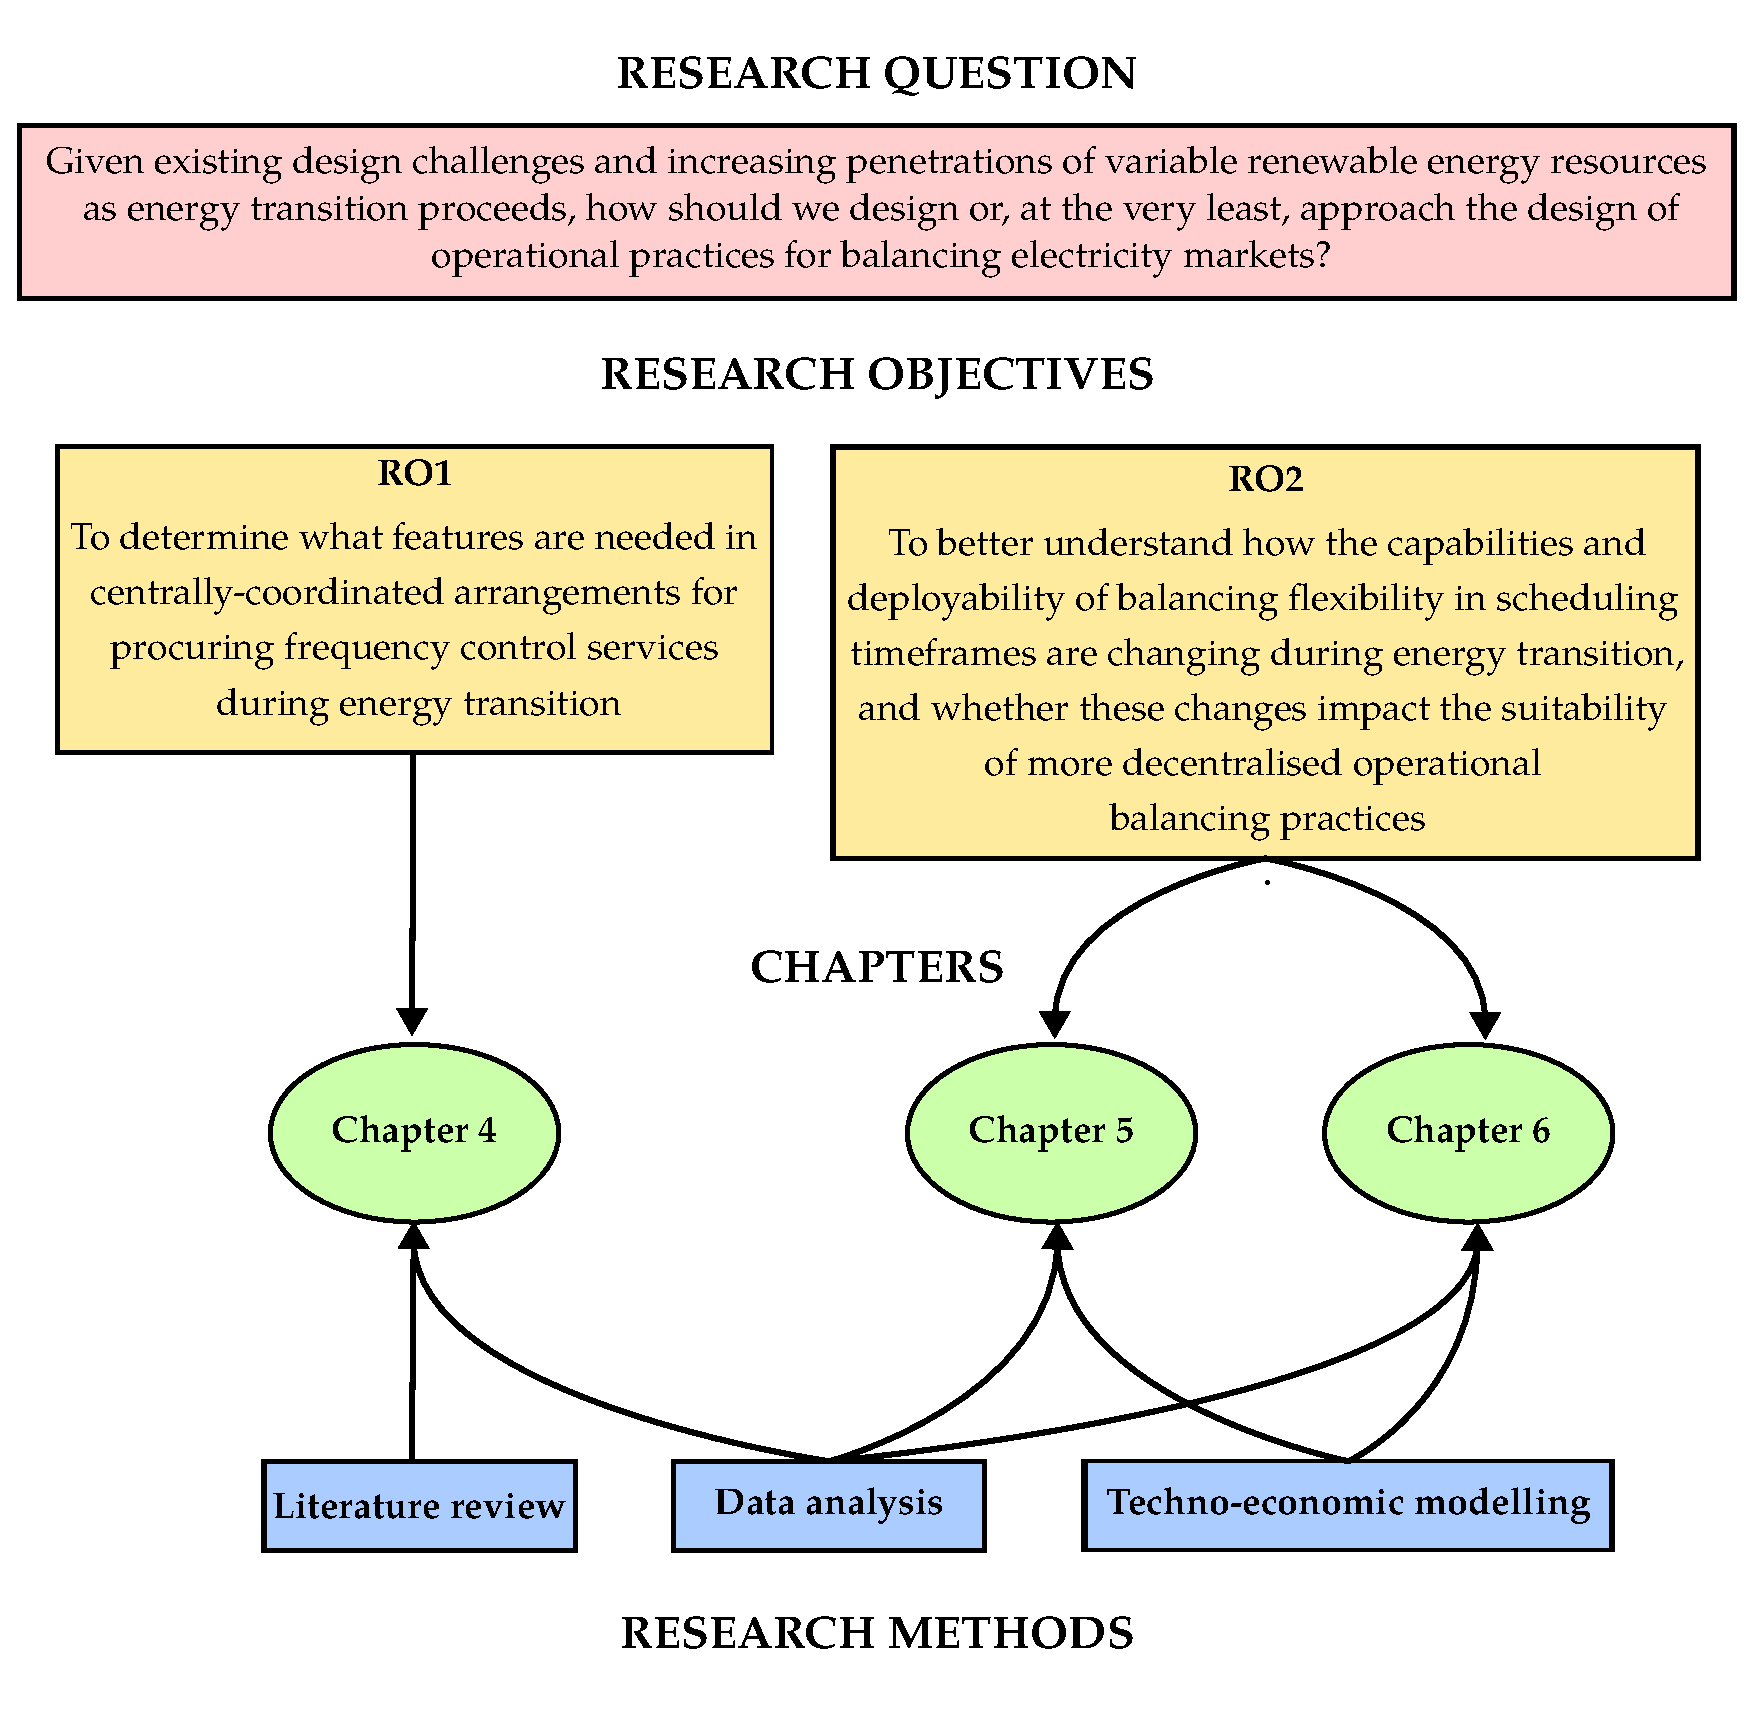
\includegraphics{source/figures/research_framework.pdf}
\caption{Research framework of this
thesis.}\label{fig:research_framework}
}
\end{figure}

\hypertarget{research-question-and-objectives}{%
\section{Research question and
objectives}\label{research-question-and-objectives}}

The research question that this thesis aims to address is outlined
below:

\begin{quote}
\emph{Given existing design challenges and increasing penetrations of
variable renewable energy resources as energy transition proceeds, how
should we design or, at the very least, approach the design of
operational practices for balancing electricity markets?}
\end{quote}

As the full scope of this research question is not possible to address
within a single doctoral thesis, I focus on aspects of the design
problem that are encompassed by the two following research objectives:

\hypertarget{research-objective-1}{%
\subsection{Research Objective 1}\label{research-objective-1}}

\begin{quote}
\emph{To determine what features are needed in centrally-coordinated
arrangements for procuring frequency control services during energy
transition.}
\end{quote}

Frequency control services are a significant component of a system
operator's balancing toolkit and are critical to ensuring that
imbalances are quickly addressed. The design of frequency control
arrangements in restructured electricity industries will need to be
revisited as resource mixes, network topologies and broader market
arrangements and policy settings change with growing penetrations of
variable renewable energy resources. Few of the studies that examine the
changes required in frequency control arrangements during energy
transition consider the design problem through both an engineering and
economics lens, and even fewer draw on past experience with existing
practices to inform future design.

Chapter \ref{sec:fcs} aims to address these shortcomings in the existing
literature and provide a perspective on what features are desirable in
the market-based frequency control arrangements as jurisdictions
decarbonise. In this chapter, I first conduct an international
literature review to provide a high-level overview and comparison of the
key features of frequency control arrangements in North America and
Central and Western Europe, and to identify the most prominent
challenges to designing effective and efficient frequency control
arrangements and potential solutions to these challenges. Then, through
another literature review and data analysis, I provide an overview and
assessment of frequency control arrangements in Australia's National
Electricity Market, which, despite long-standing frequency control
ancillary services markets, has had recent challenges in maintaining
secure frequency control. I assess the performance of evolving
arrangements in the NEM in delivering improved frequency control
outcomes, with particular regard to growing renewable penetrations and
evident tensions between mandatory requirements and market-based
incentives. Based on this assessment, I discuss the trade-offs between
effective and efficient outcomes, and provide arguments for more robust
and forward-looking frequency control arrangements during energy
transition. Finally, I draw out four key insights on designing frequency
control arrangements as power system capabilities and needs change: 1)
Understanding control action interactions, 2) implementing efficient
price formation and cost-allocation mechanisms, 3) monitoring and
assessing service provision to better align participant remuneration
with service quality, and 4) considering both regulatory and market
mechanisms and their consequences and interactions.

\hypertarget{research-objective-2}{%
\subsection{Research Objective 2}\label{research-objective-2}}

\begin{quote}
\emph{To better understand how the \textbf{capabilities} and
\textbf{deployability} of balancing flexibility in scheduling timeframes
are changing during energy transition, and whether these changes impact
the suitability of more decentralised operational balancing practices.}
\end{quote}

In wholesale electricity markets, market participation decisions
determine the type and quantity of balancing flexibility available
within scheduling timeframes. There is a role for empirical studies
examining whether decentralised operational balancing practices, such as
markets for services and products, are purpose-fit to deliver the
balancing flexibility requirements of electricity markets in transition
-- particularly given that new markets for flexibility (e.g.~reserve
product markets) can introduce additional costs, constraints and
complexity, and even encroach upon the functions of existing operational
practices. Chapter \ref{sec:reserves} focuses on understanding balancing
flexibility \textbf{capabilities} in scheduling timeframes both now and
into the near future, and using this knowledge to inform market design.
In this chapter, I offer a practical method for quantifying the
time-varying spectrum of upwards and downwards balancing flexibility
capabilities, and then use this method to assess historical and
projected resource mixes in two regions of the Australian National
Electricity Market. The results from my analysis suggest that with
higher penetrations of renewable energy: 1) downwards flexibility
margins can be exhausted around noon if wind and solar are unable or
unwilling to provide it, 2) upwards flexibility becomes more scarce
during morning and evening peak demand events and 3) a greater portion
of upwards flexibility is provided by energy-limited resources. Using
these findings, I examine and compare the suitability of various
flexibility design options, with a particular focus on assessing the
need for an additional reserve product market. I recommend that
policy-makers examine how existing operational practices can be
augmented to elicit upwards flexibility provision, and that duration
specifications and sustained footroom procurement be considered for
reserve products.

Simply quantifying capabilities, however, is insufficient if market
participants are unable or unwilling to offer them into the wholesale
spot market. Market participation decisions and thus resource schedules
are informed by knowledge processes, which provide current and
forecasted power system and market information. As such these knowledge
processes and, more broadly, market participation rules must be
purpose-fit to enable resource scheduling that leads to effective and
efficient system balancing. Chapter \ref{sec:info} explores how market
information and market participant operational strategies impact the
\textbf{deployability} of balancing flexibility from energy-limited
storage resources, which are expected to aid in balancing electricity
markets with high penetrations of variable renewable energy through
energy arbitrage. In this chapter, I focus on the scheduling
coordination role of centralised price forecasts generated by the system
and market operator in Australian National Electricity Market. I
highlight the increasing frequency and severity of errors in these price
forecasts, and propose a hypothesis that market participant (re)bidding
is partially responsible for this phenomenon. I then model the extent to
which arbitrage revenues might be reduced (compared to perfect foresight
operation) should these forecasts guide battery energy storage
scheduling. Based on the findings from these analyses, I discuss
potential changes to market participant scheduling strategies and market
design that could improve scheduling outcomes. I recommend that
Australian policy-makers not only increase the frequency at which
centralised knowledge processes are run, but also consider whether
stricter market participation restrictions might incentivise participant
bidding strategies that are less likely to induce sudden price forecast
swings that can hamper effective scheduling.

\hypertarget{case-studies-of-the-australian-national-electricity-market}{%
\subsection{Case studies of the Australian National Electricity
Market}\label{case-studies-of-the-australian-national-electricity-market}}

Whilst this thesis aims to achieve these research objectives and thus
produce insights for policy-makers worldwide, I draw on experiences from
the Australian NEM and use its resource configurations and market
arrangements in the case studies contained within this thesis. Research
from the NEM should be interesting and applicable to electricity market
designers elsewhere for several reasons:

\begin{enumerate}
\def\labelenumi{\arabic{enumi}.}
\tightlist
\item
  Relative to other jurisdictions, the NEM regularly experiences high
  instantaneous penetrations of renewable energy (a maximum of 72.9\% in
  November 2023\footnote{Maximum as of the time of writing. Figure
    obtained using GPE NEMLog
    (\protect\hyperlink{ref-globalpowerenergyWelcomeGPENEMLog22023}{Global
    Power Energy, 2023}).}) and variable renewable energy (a maximum of
  71.9\% in November 2023\footnote{Maximum as of the time of writing.
    Figure obtained using GPE NEMLog
    (\protect\hyperlink{ref-globalpowerenergyWelcomeGPENEMLog22023}{Global
    Power Energy, 2023}).}). As such, the changes in balancing
  flexibility capabilities and requirements in the NEM that are
  discussed in this thesis foreshadow those that are likely to occur in
  other jurisdictions as they decarbonise their electricity supply.
\item
  Similarly, the NEM has seen world-leading deployments of rooftop solar
  PV and other consumer-owned energy resources. These resources
  constitute a significant part of the resource mix (as high as 48\% in
  a single market interval in October 2023\footnote{Maximum as of the
    time of writing. Figure obtained using GPE NEMLog
    (\protect\hyperlink{ref-globalpowerenergyWelcomeGPENEMLog22023}{Global
    Power Energy, 2023}).}). Electricity market designers worldwide are
  becoming increasingly concerned with the impact of these resources on
  system balancing and are considering how best to facilitate the
  provision of balancing flexibility from these resources to the benefit
  of both the system and consumers. In this thesis, I touch on the
  impact of consumer-owned energy resources on balancing, and which
  operational features and practices best enable these resources to
  offer balancing flexibility to the wider system. However, distributed
  and consumer-owned energy resources are not a focus of this thesis.
\item
  Many of the world's electricity markets are considering or adopting
  design features, such as short market intervals and faster frequency
  control service markets, that have long been a part of the NEM's
  design. As such, the experience from the NEM outlined in this thesis
  can inform how or whether certain design features should be
  implemented elsewhere.
\end{enumerate}

\hypertarget{research-methods}{%
\section{Research methods}\label{research-methods}}

To achieve the objectives outlined in the previous subsection, I use the
following research methods:

\hypertarget{literature-review}{%
\subsection{Literature review}\label{literature-review}}

Academic and industry literature on operational balancing practices from
the NEM and other jurisdictions was reviewed to better understand the
nature of the design problem and the success of, as well as remaining
challenges with, the implementation of various balancing practices.
Though a detailed literature review was completed for each study, a
large portion of the output from the literature review is in Chapter
\ref{sec:fcs}. The review demonstrated that though some challenges are
universal, solutions must be tailored to each context given the
diversity of system outcomes and operational practice configurations
across jurisdictions worldwide (a challenge described in
Section~\ref{sec:lit_review-design_challenges}).

\hypertarget{system-and-market-data-analysis}{%
\subsection{System and market data
analysis}\label{system-and-market-data-analysis}}

Various analyses of system and market data from the Australian NEM were
completed in Chapters \ref{sec:fcs}, \ref{sec:reserves} and
\ref{sec:info} to assess system and market outcomes, and to provide
empirical evidence for market modelling assumptions (next subsection)
and policy discussion in this thesis. Data was obtained using
NEM-specific open-source packages including \texttt{NEMOSIS}
(\protect\hyperlink{ref-gormanNEMOSISNEMOpen2018}{Gorman et al., 2018}),
\texttt{NEMSEER}
(\protect\hyperlink{ref-prakashNEMSEERPythonPackage2023}{Prakash et al.,
2023b}), the \texttt{AEMO\ Monthly\ Data\ Archive} tool
(\protect\hyperlink{ref-prakashAEMOMonthlyData2023}{Prakash, 2023a}) and
\texttt{nem-bidding-dashboard}
(\protect\hyperlink{ref-gormanNembiddingdashboard2023}{Gorman and
Chambers, 2023}), and analysed in Python and Julia
(\protect\hyperlink{ref-bezansonJuliaFreshApproach2017}{Bezanson et al.,
2017}) using \texttt{pandas}
(\protect\hyperlink{ref-reback2020pandas}{The pandas development team,
2020}) and \texttt{DataFrames.jl}
(\protect\hyperlink{ref-juliadataDataFramesJl2023}{JuliaData, 2023}) ,
respectively. Plots were generated using \texttt{matplotlib}
(\protect\hyperlink{ref-hunterMatplotlib2DGraphics2007}{Hunter, 2007}),
\texttt{plotly}
(\protect\hyperlink{ref-plotlytechnologiesinc.CollaborativeDataScience2015}{Plotly
Technologies Inc., 2015}) or \texttt{Makie.jl}
(\protect\hyperlink{ref-danischMakieJlFlexible2021}{Danisch and
Krumbiegel, 2021}).

\hypertarget{techno-economic-market-modelling}{%
\subsection{Techno-economic (market)
modelling}\label{techno-economic-market-modelling}}

Techno-economic optimisation modelling was completed as a part of the
work presented in Chapters \ref{sec:reserves} and \ref{sec:info}. In
Chapter \ref{sec:reserves}, two market regions of the Australian NEM
were modelled using PLEXOS, a commercial power system and electricity
market modelling tool
(\protect\hyperlink{ref-energyexemplarPLEXOSEnergyMarket2021}{Energy
Exemplar, 2021}). It enables scheduling processes and bid-based
electricity markets to be modelled. The longer-term scheduling and
market modelling problems formulated by PLEXOS were solved using the
CPLEX solver (\protect\hyperlink{ref-ibmCPLEXOptimizer2021}{IBM, 2021}).
In Chapter \ref{sec:info}, an open-source Julia optimisation package
(\texttt{JuMP}) was used to formulate mixed-integer linear programs that
were then solved to produce market participation schedules for energy
storage resources with different storage durations and operational
objectives
(\protect\hyperlink{ref-lubinJuMPRecentImprovements2023}{Lubin et al.,
2023}). Each of the optimisation problems was solved using the
open-source HiGHs solver
(\protect\hyperlink{ref-huangfuParallelizingDualRevised2018}{Huangfu and
Hall, 2018}) on Katana, a high-performance computational cluster
supported by UNSW Research Technology Services
(\protect\hyperlink{ref-unswresearchtechnologyservicesKatana2023}{UNSW
Research Technology Services, 2023}). Results from Chapter
\ref{sec:reserves} were analysed using \texttt{pandas}
(\protect\hyperlink{ref-reback2020pandas}{The pandas development team,
2020}) and plotted using \texttt{matplotlib}
(\protect\hyperlink{ref-hunterMatplotlib2DGraphics2007}{Hunter, 2007}),
and results from Chapter \ref{sec:info} were analysed using
\texttt{DataFrames.jl}
(\protect\hyperlink{ref-juliadataDataFramesJl2023}{JuliaData, 2023}) and
plotted using \texttt{Makie.jl}
(\protect\hyperlink{ref-danischMakieJlFlexible2021}{Danisch and
Krumbiegel, 2021}).

\hypertarget{sec:fcs}{%
\chapter{Frequency control arrangements: insights from the National
Electricity Market}\label{sec:fcs}}

\hypertarget{link-to-thesis}{%
\section{Link to thesis}\label{link-to-thesis}}

Frequency control services are a significant component of a system
operator's balancing toolkit and are critical to ensuring that
imbalances are quickly addressed. The design of frequency control
arrangements in restructured electricity industries will need to be
revisited as resource mixes, network topologies and broader market
arrangements and policy settings change with growing penetrations of
variable renewable energy resources. This chapter aims to provide a
perspective on what features are desirable in the market-based frequency
control arrangements as jurisdictions decarbonise by drawing on
experiences from the Australian National Electricity Market. The purpose
of this chapter is to address the first research objective of this
thesis (see Section~\ref{sec:research_framework}).

The content of this chapter is from the following peer-reviewed journal
article published in \emph{Renewable and Sustainable Energy Reviews}:

\textbf{Prakash, A.}, Bruce, A. \& MacGill, I. Insights on designing
effective and efficient frequency control arrangements from the
Australian National Electricity Market. Renewable and Sustainable Energy
Reviews 161, 112303 (2022).

\hypertarget{abstract-1}{%
\section{Abstract}\label{abstract-1}}

For restructured electricity industries undergoing energy transition,
designing effective and efficient frequency control arrangements is a
complex and ongoing task that requires appropriate configuration of
controllers, generator technical connection requirements, market
arrangements and wider policy settings. In this paper, we provide an
overview and assessment of these arrangements in Australia's National
Electricity Market - a useful case study given its long-standing
frequency control ancillary services markets, yet recent challenges in
maintaining secure frequency control. We assess the performance of these
evolving arrangements in delivering improved frequency control outcomes,
with particular regard to growing renewable penetrations and evident
tensions between mandatory requirements and market-based incentives.
Based on this assessment, we draw out four key insights on designing
frequency control arrangements as power system capabilities and needs
change: 1) Understanding control action interactions, 2) Implementing
efficient price formation and cost-allocation mechanisms, 3) Monitoring
and assessing service provision to better align participant remuneration
with service quality, and 4) Considering both regulatory and market
mechanisms and their consequences and interactions. In particular, we
discuss the trade-offs between effective and efficient outcomes, and
provide arguments for more robust and forward-looking frequency control
arrangements during energy transition.

\hypertarget{sec:fcs-intro}{%
\section{Introduction}\label{sec:fcs-intro}}

As a consequence of growing momentum to address global warming and
continually declining technology costs, many power systems around the
world are undergoing an energy transition in which significant capacity
additions of variable renewable energy (VRE) and other inverter-based
resources (IBR) are being accompanied by the progressive retirement of
existing fossil fuel generation
(\protect\hyperlink{ref-internationalenergyagencyNetZero20502021}{International
Energy Agency, 2021}). Such power systems are currently experiencing or
expected to soon experience high instantaneous penetrations of VRE
(i.e.~beyond 50\% of grid demand being met by VRE at any given time),
which can pose technical challenges to the stable and secure operation
of a power system
(\protect\hyperlink{ref-kenyonStabilityControlPower2020}{Kenyon et al.,
2020};
\protect\hyperlink{ref-kroposkiAchieving100Renewable2017}{Kroposki et
al., 2017};
\protect\hyperlink{ref-meegahapolaPowerSystemStability2021}{Meegahapola
et al., 2021}). While several of these challenges have technological
solutions of various maturities, configuring mechanisms in an effective
and efficient manner across power system design layers, which span from
how resources are controlled to how grid codes and markets are designed,
remains an open and significant challenge.

In this article, we focus on one aspect of power system security:
control of AC frequency. Maintaining frequency near the nominal value of
a power system (either 50 or 60 Hz) is contingent on the ongoing balance
of active power supply and demand within a synchronous area
(\protect\hyperlink{ref-graingerPowerSystemAnalysis1994}{Grainger,
1994}). Power system frequency deviations are a consequence of
instantaneous supply-demand imbalances, which typically occur as a
result of system variability (predictable changes in supply or demand,
such as fluctuations and ramps of generation or load) and uncertainty
(unpredicted changes in supply or demand, such as forecast errors or
unplanned outages)
(\protect\hyperlink{ref-elaOperatingReservesVariable2011}{Ela et al.,
2011}). System operators (SOs) achieve short-term active power balancing
using reserve capacity. Whilst there are many names for these
reserves\footnote{The term \emph{balancing services} is used in European
  systems, whereas the term \emph{operating reserves} is widely used in
  North America.}, this article will focus on a common subset that
responds to and mitigates frequency deviations over short timeframes
(milliseconds to minutes). We will refer to such reserves as
\emph{Frequency Control Services} (FCS). If FCS are insufficient or
inadequate, the system frequency may deviate beyond acceptable system
limits and lead to equipment damage, load shedding, generator trips and
cascading failures that lead to blackouts
(\protect\hyperlink{ref-kirbyFrequencyControlConcerns2002}{Kirby et al.,
2002}; \protect\hyperlink{ref-ulbigImpactLowRotational2014}{Ulbig et
al., 2014}).

In electricity industries with competitive markets for energy and FCS,
frequency control arrangements consist of control, regulatory and
market-based mechanisms
(\protect\hyperlink{ref-mancarellaFragileGridPhysics2021}{Mancarella and
Billimoria, 2021}). Control mechanisms specify the technical
requirements for FCS. Regulatory and market-based mechanisms are used by
the SO to:

\begin{enumerate}
\def\labelenumi{\arabic{enumi}.}
\item
  Mandate or incentivise participant behaviour in the energy market that
  facilitates system balancing. This includes enforcing dispatch
  compliance or penalising participant portfolio imbalances; and
\item
  Procure FCS from capable resources (i.e.~generators, loads and network
  elements).
\end{enumerate}

Regulatory FCS procurement mechanisms are often mandatory and include
equipment standards, connection requirements and SO intervention,
whereas market-based FCS procurement mechanisms are often voluntary and
include remunerative schemes and contract or spot markets. Together,
these mechanisms dictate the physical effectiveness and productive,
dynamic, price formation and cost-allocation efficiencies of FCS
provision and procurement. Well-designed arrangements should be
effective and efficient, where \emph{effectiveness} entails sufficient
and robust frequency response to meet physical power system requirements
and \emph{efficiency} relates to frequency response being provided at
low cost, both now and into the future
(\protect\hyperlink{ref-reboursFundamentalDesignIssues2007}{Y. Rebours
et al., 2007};
\protect\hyperlink{ref-vanderveenElectricityBalancingMarket2016}{van der
Veen and Hakvoort, 2016}).

As power systems transition towards higher instantaneous penetrations of
VRE and IBR, SOs are likely to face the following challenges to
short-term system balancing that may require existing frequency control
arrangements to be revisited:

\begin{itemize}
\item
  VRE adds variability and uncertainty to a power system, particularly
  if similar technologies are situated within close proximity of one
  another (i.e.~correlated production and/or forecast errors)
  (\protect\hyperlink{ref-australianenergymarketoperatorRenewableIntegrationStudy2020}{Australian
  Energy Market Operator, 2020a};
  \protect\hyperlink{ref-keeratimahatAnalysisShorttermOperational2021}{Keeratimahat
  et al., 2021}). Furthermore, unless an appropriate response is
  incorporated and enabled in their control systems, VRE and other IBR
  do not provide FCS. In jurisdictions that do not require, incentivise
  or allow VRE and IBR to provide FCS, the displacement of synchronous
  machines in dispatch has led to lower availabilities of resources that
  provide FCS
  (\protect\hyperlink{ref-australianenergymarketoperatorRenewableIntegrationStudy2020c}{Australian
  Energy Market Operator, 2020e};
  \protect\hyperlink{ref-denholmInertiaPowerGrid2020}{Denholm et al.,
  2020};
  \protect\hyperlink{ref-milanoFoundationsChallengesLowInertia2018}{Milano
  et al., 2018}) .
\item
  In jurisdictions with competitive markets for energy and FCS, there is
  a tension between achieving economically efficient markets and the
  redundancy, certainty and control afforded to the SO. While the
  societal and economic costs of power system failure are often very
  large, it may be difficult for the SO to justify the cost of
  mitigation measures when they are ongoing or significant and when the
  joint probability of events or failures is low. The uncertainties
  associated with energy transition and the impacts of global warming
  are likely to present additional challenges. Power system security
  measures may need to be implemented rapidly and be both robust to a
  range of futures and resilient in the face of shocks, such as severe
  weather events
  (\protect\hyperlink{ref-egglestonSecurityResilienceTechnical2021}{Eggleston
  et al., 2021};
  \protect\hyperlink{ref-prakashResponseFrequencyControl2021}{Prakash et
  al., 2021}).
\end{itemize}

In this paper, we provide insights and recommendations on designing more
effective and efficient frequency control arrangements based on
experience from the Australian National Electricity Market (NEM). The
NEM is currently experiencing relatively high system-wide instantaneous
VRE penetrations (just over 60\% in 2021) and is expected to experience
penetrations as high as 75-100\% by 2025
(\protect\hyperlink{ref-australianenergymarketoperatorNEMEngineeringFramework2021}{Australian
Energy Market Operator, 2021b},
\protect\hyperlink{ref-australianenergymarketoperatorQuarterlyEnergyDynamics2021}{2021c}).
Though the NEM's frequency control arrangements were once arguably
world-leading
(\protect\hyperlink{ref-rieszFrequencyControlAncillary2015}{Riesz et
al., 2015};
\protect\hyperlink{ref-thorncraftExperienceMarketbasedAncillary2007}{Thorncraft
and Outhred, 2007}), the speed at which system capabilities and needs
are changing and the removal of mandatory requirements in 2001 as a part
of a paradigm shift from obligation to remuneration for FCS have exposed
design issues. In attempting to address these issues, the NEM's rule
makers have placed FCS obligations on generators and transmission
network operators and have undertaken reforms to the NEM's energy and
FCS markets, including introducing a new market to procure emergency
fast frequency response (FFR) from IBR. Whilst the NEM is an
electrically-isolated power system with a relatively simple energy-only
market, the insights and recommendations from this paper are likely to
be relevant to other power systems and interconnections as their
existing conventional generation retires and VRE deployment levels
increase.

This paper offers three contributions to the literature. First, we
provide a high-level overview and comparison of the key features of
frequency control arrangements in North America and Central and Western
Europe, and provide a review of the most prominent challenges to
designing effective and efficient frequency control arrangements and the
potential solutions discussed in the literature. Second, we provide a
comprehensive update to previous literature on frequency control in the
NEM (\protect\hyperlink{ref-rieszFrequencyControlAncillary2015}{Riesz et
al., 2015};
\protect\hyperlink{ref-thorncraftMarketbasedAncillaryServices2008}{Thorncraft
et al., 2008};
\protect\hyperlink{ref-thorncraftExperienceMarketbasedAncillary2007}{Thorncraft
and Outhred, 2007}). Our analysis benefits from recent experience in the
NEM that encompasses deteriorating frequency performance, the
reintroduction of mandatory requirements and integrating higher shares
of VRE. While several of these aspects have been discussed independently
in the literature, this paper seeks to provide a structured and holistic
analysis of developments in the NEM and their implications for frequency
control arrangement design. Third, this article advocates for designers
placing a greater emphasis on delivering forward-looking frequency
control arrangements during energy transition through the implementation
of more robust regulatory mechanisms and ensuring that market-based
mechanisms are capable of supporting FCS investment. As highlighted in
the following sections, these design features have received surprisingly
little attention in the literature.

The rest of the chapter is structured as follows. In
Section~\ref{sec:fcs-context}, we provide an overview of typical
frequency control arrangements, with a focus on restructured electricity
industries in North America and Europe, and the main challenges faced in
their design. We describe the NEM, its frequency control arrangements
and the specific challenges posed by increasing penetrations of VRE and
other IBR in Section~\ref{sec:fcs-nem}. In
Section~\ref{sec:fcs-insights}, we analyse the performance of the NEM's
frequency control arrangements in responding to the challenges explored
in Section~\ref{sec:fcs-context}, with primary frequency response and
regulation (secondary frequency response) services in the NEM as case
studies. Based on our analysis, we conclude by offering four key
insights to operators, regulators and market-bodies that include
understanding control action interactions; ensuring that arrangements
are capable of supporting investment in FCS capability; monitoring,
assessing and remunerating FCS performance; and considering both
regulatory and market-based mechanisms in the design of effective and
efficient frequency control arrangements.

\hypertarget{sec:fcs-context}{%
\section{Context}\label{sec:fcs-context}}

\hypertarget{conventional-frequency-control-schemes}{%
\subsection{Conventional frequency control
schemes}\label{conventional-frequency-control-schemes}}

SOs employ hierarchical and sequential frequency control schemes. In
most power systems, such schemes implicitly include inertial response
and explicitly define FCS such as primary frequency response (PFR),
secondary frequency response (SFR) and tertiary frequency response
(TFR). In general, once frequency has deviated from the system nominal
value, synchronous machines provide an inertial response that is
inherent and immediate in slowing the rate of change of frequency
(RoCoF). Within seconds, generators and/or loads provide autonomous and
decentralised control action through PFR
(\protect\hyperlink{ref-etoFrequencyControlRequirements2018}{Eto et al.,
2018};
\protect\hyperlink{ref-machowskiPowerSystemDynamics2020}{Machowski et
al., 2020}). PFR arrests the frequency deviation to enable the slower
and more centralised control actions of SFR and TFR to return the power
system frequency to its nominal value
(\protect\hyperlink{ref-elaAlternativeApproachesIncentivizing2012}{Ela
et al., 2012b}; \protect\hyperlink{ref-etoUseFrequencyResponse2010}{Eto
et al., 2010}). Should system frequency continue to rise or fall beyond
the system's allowable limits, emergency protection schemes such as
under-frequency load shedding (UFLS) and over-frequency generation
shedding (OFGS) relays may be triggered. In some systems, RoCoF relays
are also used to prevent high RoCoFs from tripping or damaging equipment
and to contain frequency nadirs and zeniths
(\protect\hyperlink{ref-akramEnergyStorageShortTerm2020}{Akram et al.,
2020};
\protect\hyperlink{ref-dgaconsultingInternationalReviewFrequency2016}{DGA
Consulting, 2016};
\protect\hyperlink{ref-millerAdvisoryEquipmentLimits2017}{Miller et al.,
2017a}).

\hypertarget{sec:fcs-context-procurement}{%
\subsection{Procurement of frequency control
services}\label{sec:fcs-context-procurement}}

Except for inertial response from synchronous machines, the SO procures
FCS capacity from capable resources within its control area and, in the
case of SFR and TFR, activates FCS energy if necessary. In electricity
industries where the SO owns most if not all the generation assets
(i.e.~a vertically-integrated utility), the SO is able to jointly
schedule generation and FCS capacity with knowledge of the condition of
the system and the status and cost structures of their plant. However,
many electricity industries have undergone some degree of restructuring,
which has created a greater role for competitively-oriented
decentralised decision-making
(\protect\hyperlink{ref-vanderveenElectricityBalancingMarket2016}{van
der Veen and Hakvoort, 2016}) . The diverse outcomes of restructuring
processes and differences in technical characteristics
(e.g.~capabilities of resource mix and network topology) have led to a
wide range of frequency control arrangements across power systems
(\protect\hyperlink{ref-poplavskayaDistributedEnergyResources2019}{Poplavskaya
and de Vries, 2019};
\protect\hyperlink{ref-reboursFundamentalDesignIssues2007}{Y. Rebours et
al., 2007}) , which have been reviewed and compared extensively within
industry and academic literature
(\protect\hyperlink{ref-banshwarInternationalExperienceTechnical2018}{Banshwar
et al., 2018};
\protect\hyperlink{ref-brooksReviewFrequencyRegulation2019}{Brooks and
Lesieutre, 2019};
\protect\hyperlink{ref-elaAncillaryServicesUnited2019}{Ela and Hytowitz,
2019};
\protect\hyperlink{ref-hewickerDimensioningControlReserves2020}{Hewicker
et al., 2020};
\protect\hyperlink{ref-lopezSurveyAssessmentTechnical2020}{Lopez et al.,
2020}; \protect\hyperlink{ref-ockerDesignEuropeanBalancing2016}{Ocker et
al., 2016};
\protect\hyperlink{ref-reboursSurveyFrequencyVoltage2007a}{Y. G. Rebours
et al., 2007a},
\protect\hyperlink{ref-reboursSurveyFrequencyVoltage2007}{2007b};
\protect\hyperlink{ref-reishusconsultingllcElectricityAncillaryServices2017}{Reishus
Consulting LLC, 2017};
\protect\hyperlink{ref-zhouSurveyAncillaryServices2016}{Zhou et al.,
2016}).

In restructured electricity industries, the provision of more passive
FCS (e.g.~ride-through capabilities) is usually mandated by regulatory
mechanisms such as connection agreements and grid codes, whereas FCS
that require additional response capabilities or impose
opportunity-costs on suppliers are procured and remunerated by the SO
through market-based mechanisms. In Section~\ref{sec:fcs-NA} \&
Section~\ref{sec:fcs-EU}, we provide an overview of typical
features\footnote{We note that there are numerous differences between
  jurisdictional arrangements and terminology in each of these regions.
  For a more general overview of potential procurement models, refer to
  Billimoria et al.
  (\protect\hyperlink{ref-billimoriaMarketDesignSystem2020}{2020}).} and
key developments in market-based mechanisms for procuring FCS in North
America and Central and Western Europe, respectively. These regions best
represent the two prevailing short-term wholesale electricity market
models: central dispatch markets, in which the SO issues dispatch
instructions, and decentralised or self-dispatch markets, in which
resource dispatch is managed by market participants
(\protect\hyperlink{ref-ahlqvistCentralSelfDispatchElectricity2018}{Ahlqvist
et al., 2018}). Given that FCS and energy are partially substitutable
goods, the characteristics of short-term wholesale electricity markets
heavily influence the design of FCS arrangements and thus these regions
provide an interesting contrast. However, despite their differences, the
SO plays a central role in both of these regions as they determine the
area demand for FCS capacity, activate FCS energy as required and are
ultimately responsible for ensuring that the power system is balanced
and securely operated.

\hypertarget{sec:fcs-NA}{%
\subsubsection{North American markets}\label{sec:fcs-NA}}

In North America, central dispatch wholesale electricity markets are
operated by an Independent System Operator (ISO) or Regional
Transmission Organization (RTO) and are distributed across three
synchronous areas. These markets consist of two short-term centralised
platforms: a day-ahead market and a real-time market. In the day-ahead
market, the SO solves a security-constrained unit commitment problem
using supply offers (single or three-part) and demand bids (quantity or
price-quantity) to produce day-ahead locational marginal prices and a
financially-binding hourly schedule. In the real-time market, the SO
solves a security-constrained economic dispatch problem (typically every
five minutes) using generator price-quantity offers and a demand
forecast to produce real-time locational marginal prices and a set of
physically and financially binding dispatch instructions. Thus, each
short-term market is cleared to maximise social welfare whilst
respecting network and system security constraints
(\protect\hyperlink{ref-chowElectricityMarketDesign2005}{Chow et al.,
2005};
\protect\hyperlink{ref-cramtonElectricityMarketDesign2017}{Cramton,
2017}).

Except for Frequency Responsive Reserves (i.e.~PFR), operating reserves
(i.e.~FCS capacity) are explicitly procured by placing an obligation on
load-serving entities to self-provide or purchase their share from
SO-run FCS markets
(\protect\hyperlink{ref-elaAlternativeApproachesIncentivizing2012}{Ela
et al., 2012b};
\protect\hyperlink{ref-zhouSurveyAncillaryServices2016}{Zhou et al.,
2016}). These FCS markets are usually integrated into day-ahead market
and, in most jurisdictions, the real-time market. Standard products in
North American markets include Regulation (i.e.~SFR during normal
operation), Spinning and Non-Spinning Reserves (i.e.~TFR deployed
following an event)
(\protect\hyperlink{ref-elaAncillaryServicesUnited2019}{Ela and
Hytowitz, 2019};
\protect\hyperlink{ref-hewickerDimensioningControlReserves2020}{Hewicker
et al., 2020};
\protect\hyperlink{ref-zhouSurveyAncillaryServices2016}{Zhou et al.,
2016}). Participants can submit offers for FCS in addition to offer for
energy. Unit commitment and economic dispatch permit co-optimisation of
energy and FCS procurement. From the perspective of the SO,
co-optimisation ensures that the total system cost of achieving an
energy supply-demand balance is minimised alongside FCS requirements,
subject to network and system security constraints. From the perspective
of participants, co-optimisation leads to an FCS price that not only
reflects the price offer of the marginal resource, but also any "profit"
it forgoes in the energy market (assuming supplier offers reflect their
short-run marginal costs)
(\protect\hyperlink{ref-elaEffectiveAncillaryServices2012}{Ela et al.,
2012a};
\protect\hyperlink{ref-isemongerEvolvingDesignRTO2009}{Isemonger,
2009}). As such, ISO/RTO FCS markets can compensate opportunity-costs
related to the day-ahead and/or real-time market but only allocate costs
to load-serving entities through a procurement obligation.

Though North American FCS markets have predominantly procured and
remunerated FCS capacity, ISO/RTOs (except Texas' ISO, ERCOT) were
ordered to also remunerate Regulation providers for the quantity of
energy provided whilst accurately following control signals by the
Federal Energy Regulatory Commission's (FERC) Order 755
(\protect\hyperlink{ref-federalenergyregulatorycommissionfercOrderNo7552011}{Commission,
2011}). As such, Regulation providers offer a quantity of capacity, a
price for capacity and a price for "mileage", which is the energy
delivered. Remuneration for Regulation takes performance (the ability of
a resource to follow the ISO/RTO's control signals) into account, though
how this is implemented varies between ISO/RTOs
(\protect\hyperlink{ref-elaAncillaryServicesUnited2019}{Ela and
Hytowitz, 2019};
\protect\hyperlink{ref-fernandez-munozFastFrequencyControl2020}{Fernández-Muñoz
et al., 2020}). A notable example is the PJM RTO, which uses both a
standard SFR control signal (RegA) and faster SFR control signal (RegD)
intended for battery energy storage systems (BESS). PJM determines how
interchangeable a resource's RegD provision is with RegA provision (the
marginal benefit factor) to clear the Regulation market and calculates a
performance score for use in market clearing and settlement. However,
according to the independent market monitor, the omission of the
marginal benefit factor from market settlement has led to perverse
market outcomes
(\protect\hyperlink{ref-brooksReviewFrequencyRegulation2019}{Brooks and
Lesieutre, 2019};
\protect\hyperlink{ref-monitoringanalytics2021QuarterlyState2021}{Monitoring
Analytics, 2021}).

\hypertarget{sec:fcs-EU}{%
\subsubsection{European markets}\label{sec:fcs-EU}}

Most of the electricity markets of Central and Western Europe are
self-dispatch and consist of two short-term platforms: the day-ahead
market and the intraday market, which can be continuous, composed of
frequently-run discrete auctions or a combination of the two. Each of
these platforms is coupled across the majority of market zones in
Europe, with a single price coupling algorithm used to simultaneously
clear zonal day-ahead markets and a single order book compiled to match
cross-zonal intraday orders
(\protect\hyperlink{ref-epexspotEuropeanMarketCoupling}{EPEX Spot,
n.d.}; \protect\hyperlink{ref-nemocommitteeSingleIntradayCoupling}{NEMO
Committee, n.d.}). In contrast to North American electricity markets,
the market operator is responsible for market operation and is distinct
from the Transmission System Operator (TSO). Generation and load are
managed by Balancing Responsible Parties (BRP), which must submit
binding operational schedules to the TSO ahead of delivery (often by the
day prior to delivery). As BRPs become aware of potential deviations
closer to real time (e.g.~improved forecasts), they are able to adjust
their submitted schedules (i.e.~remain "balanced") through trades on the
intraday market
(\protect\hyperlink{ref-lagoMarketFrameworkGrid2021}{Lago et al.,
2021b};
\protect\hyperlink{ref-musgensEconomicsDesignBalancing2014}{Müsgens et
al., 2014}). BRPs face financial repercussions if they are imbalanced
via an imbalance price and, in some jurisdictions, are legally obliged
to be balanced
(\protect\hyperlink{ref-entso-ewgasSurveyAncillaryServices2021}{ENTSO-E
WGAS, 2021}).

Following gate-closure of the intraday market, residual imbalances are
primarily addressed by FCS (known as balancing services) procured by the
TSO. Standard FCS in Europe include Frequency Containment Reserve
(i.e.~PFR), automatic Frequency Restoration Reserves (i.e.~SFR), and
manual Frequency Restoration Reserves and Replacement Reserves
(i.e.~both TFR), with minimum technical requirements for each specified
by the European Network of Transmission System Operators for Electricity
(ENTSO-E)
(\protect\hyperlink{ref-europeannetworkoftransmissionsystemoperatorsforelectricityentso-eNetworkCodeLoadFrequency2013}{European
Network of Transmission System Operators for Electricity, 2013}).
Depending on the FCS product and the jurisdiction, TSOs may distinguish
between FCS capacity (balancing capacity) and the delivery of FCS energy
(balancing energy). The provision of one or both is mandated in some
cases, but where both are procured competitively, Balancing Service
Providers (BSP) typically submit separate offers for FCS capacity and
FCS energy
(\protect\hyperlink{ref-abbasyNationalDesignMultinational2012}{Abbasy,
2012}). FCS capacity markets are often cleared days to months in advance
of real-time whereas the FCS energy market, which effectively
constitutes merit-order or pro rata activation of capacity for FCS
energy provision, is cleared within an hour or minutes of real-time
(\protect\hyperlink{ref-entso-ewgasSurveyAncillaryServices2021}{ENTSO-E
WGAS, 2021};
\protect\hyperlink{ref-ockerDesignEuropeanBalancing2016}{Ocker et al.,
2016};
\protect\hyperlink{ref-poplavskayaDistributedEnergyResources2019}{Poplavskaya
and de Vries, 2019}). FCS capacity costs are typically allocated to
power system users via a grid tariff. FCS energy costs are typically
allocated to BRPs based on their schedule deviations and an imbalance
price, which may differ from the FCS energy price paid to BSPs
(\protect\hyperlink{ref-hirthBalancingPowerVariable2015}{Hirth and
Ziegenhagen, 2015};
\protect\hyperlink{ref-vandezandeWellfunctioningBalancingMarkets2010}{Vandezande
et al., 2010}). As such, European FCS markets generally disincentivise
causers of imbalance through the imbalance price, which may also recover
or reflect the cost of FCS energy. However, since FCS capacity markets
are typically decoupled from and cleared ahead of short-term energy
markets, perceived opportunity-costs based on expected short-term energy
market prices must be internalised within participants' FCS offers.

Given the relatively high degree of interconnection between transmission
systems in Central and Western Europe, cross-TSO initiatives are in
place and being expanded to address imbalances and share FCS across the
Continental Europe synchronous area. When sufficient cross-TSO
transmission capacity is available, initiatives currently in place
enable participating TSOs to jointly procure Frequency Containment
Reserve capacity, net imbalances (i.e.~reduce the demand for SFR by
aggregating individual control area imbalances) and jointly procure
automatic Frequency Restoration Reserve capacity and energy
(\protect\hyperlink{ref-europeannetworkoftransmissionsystemoperatorsforelectricityentso-eENTSOEBalancingReport2020}{European
Network of Transmission System Operators for Electricity, 2020}).
Further efficiency gains are expected following the implementation of
integrated market platforms for imbalance netting and balancing energy
for SFR and TFR. The implementation of these platforms is mandated by
the European Commission's European Balancing Guideline and requires
certain FCS product definitions and market features to be harmonised
across the balancing energy markets of participating TSOs
(\protect\hyperlink{ref-50hzamprionapgeliartetennetConsultationDesignPlatform2017}{50hz,
2017};
\protect\hyperlink{ref-europeancommissionCommissionRegulationEU2017}{European
Commission, 2017}).

\hypertarget{sec:fcs-design}{%
\subsection{Designing frequency control
arrangements}\label{sec:fcs-design}}

As with any policy problem, designing frequency control arrangements in
restructured electricity industries requires design principles,
variables and performance criteria to be established. The public good
characteristics of frequency control have heavily influenced arrangement
design principles across jurisdictions, such as the common preference
for the SO to centrally coordinate FCS procurement and activation
(\protect\hyperlink{ref-musgensEconomicsDesignBalancing2014}{Müsgens et
al., 2014};
\protect\hyperlink{ref-reboursFundamentalDesignIssues2007}{Y. Rebours et
al., 2007}). In contrast, though some design variables are common,
others may only apply to particular systems based on their resource mix,
network topology and/or market design. Y. Rebours et al.
(\protect\hyperlink{ref-reboursFundamentalDesignIssues2007}{2007})
discuss design variables for central dispatch markets related to the
following arrangement features:

\begin{enumerate}
\def\labelenumi{\arabic{enumi}.}
\item
  FCS procurement;
\item
  Price formation, which when efficient should lead to FCS prices not
  only reflecting the true cost of the service, but also its true value
  to the system; and
\item
  Allocation of the cost of FCS.
\end{enumerate}

Similarly, Abbasy
(\protect\hyperlink{ref-abbasyNationalDesignMultinational2012}{2012})
discusses the main design variables applicable to European self-dispatch
markets. van der Veen and Hakvoort
(\protect\hyperlink{ref-vanderveenElectricityBalancingMarket2016}{2016})
build upon this work to provide a more comprehensive treatment of design
variables in self-dispatch markets. Y. Rebours et al.
(\protect\hyperlink{ref-reboursFundamentalDesignIssues2007}{2007}),
Abbasy
(\protect\hyperlink{ref-abbasyNationalDesignMultinational2012}{2012})
and van der Veen and Hakvoort
(\protect\hyperlink{ref-vanderveenElectricityBalancingMarket2016}{2016})
all propose some variation of effectiveness and efficiency as
performance criteria, with van der Veen and Hakvoort
(\protect\hyperlink{ref-vanderveenElectricityBalancingMarket2016}{2016})
analysing the various trade-offs between and within each criterion.

Despite the well-defined nature of the design problem, there are several
challenges to achieving effective and efficient arrangements. In
Section~\ref{sec:fcs-ibr-challenges} \&
Section~\ref{sec:fcs-efficiency-challenges}, we present the most
prominent challenges and their treatment in the literature.

\hypertarget{sec:fcs-ibr-challenges}{%
\subsubsection{The influx of VRE and other IBR in power
systems}\label{sec:fcs-ibr-challenges}}

As discussed in Section~\ref{sec:fcs-intro}, VRE adds variability and
uncertainty to power systems which, at the very least, can lead to
increased procurement and activation requirements for PFR and SFR during
normal operating conditions
(\protect\hyperlink{ref-elaOperatingReservesVariable2011}{Ela et al.,
2011}). Three proposals to address this issue and thus reduce FCS
requirements with growing penetrations of VRE have been discussed in the
literature. The first is to shorten energy market trading/dispatch
intervals (\protect\hyperlink{ref-ockerGermanParadoxBalancing2017}{Ocker
and Ehrhart, 2017};
\protect\hyperlink{ref-rieszDesigningElectricityMarkets2015}{Riesz and
Milligan, 2015}) and the time between market gate closure and dispatch
(\protect\hyperlink{ref-katzOpeningMarketsDesigning2019}{Katz et al.,
2019}), thereby enabling scheduling based on up-to-date system
conditions and forecasts. The second is to increase coordination between
control areas within a synchronous area by netting imbalances
(\protect\hyperlink{ref-kingFlexibilityReserveReductions2011}{King et
al., 2011}), jointly procuring and dispatching FCS
(\protect\hyperlink{ref-schererIntegratedPanEuropeanAncillary2013}{Scherer
et al., 2013}) or aggregating them into a single market region
(\protect\hyperlink{ref-milliganMarketCharacteristicsEfficient2010}{Milligan
and Kirby, 2010};
\protect\hyperlink{ref-rieszDesigningElectricityMarkets2015}{Riesz and
Milligan, 2015}). These two proposals alone have delivered significant
system savings in Germany despite growing penetrations of VRE
(\protect\hyperlink{ref-hirthBalancingPowerVariable2015}{Hirth and
Ziegenhagen, 2015};
\protect\hyperlink{ref-ockerGermanParadoxBalancing2017}{Ocker and
Ehrhart, 2017}). The third is for the SO to determine the required
quantity of FCS capacity (\emph{dimensioning}) using dynamic and
probabilistic approaches (as opposed to static and deterministic) that
adequately reflect current or expected power system conditions and an
acceptable level of risk, such as a reliability standard
(\protect\hyperlink{ref-devosDynamicDimensioningApproach2019}{De Vos et
al., 2019};
\protect\hyperlink{ref-holttinenMethodologiesDetermineOperating2013}{Holttinen
et al., 2013};
\protect\hyperlink{ref-ortega-vazquezRiskBasedReserveProcurement2020}{Ortega-Vazquez
et al., 2020}).

In recent years, SOs have become increasingly concerned with growing
penetrations of asynchronous IBR leading to higher RoCoFs and fewer
resources offering conventional FCS
(\protect\hyperlink{ref-denholmInertiaPowerGrid2020}{Denholm et al.,
2020};
\protect\hyperlink{ref-dgaconsultingInternationalReviewFrequency2016}{DGA
Consulting, 2016};
\protect\hyperlink{ref-hartmannEffectsDecreasingSynchronous2019}{Hartmann
et al., 2019}). However, VRE and other IBR are able to provide tunable
conventional FCS, FFR and/or an inherent response that strongly
resembles the inertial response of synchronous machines\footnote{The
  terms \emph{virtual, emulated and synthetictic} inertia have been used
  in the literature to refer to a proportional active power response to
  RoCoF. However, these terms do not distinguish whether the inverter
  control scheme provides an inherent response (i.e.~from inverters
  operated as a voltage source which are commonly referred to as
  \emph{grid-forming inverters}
  (\protect\hyperlink{ref-cherevatskiyGridFormingEnergy2020}{Cherevatskiy
  et al., 2020};
  \protect\hyperlink{ref-linResearchRoadmapGridForming2020}{Lin et al.,
  2020})) or a controlled response following frequency measurement
  (\protect\hyperlink{ref-erikssonSyntheticInertiaFast2018}{Eriksson et
  al., 2018};
  \protect\hyperlink{ref-tielensRelevanceInertiaPower2016}{Tielens and
  Van Hertem, 2016}).} if this is facilitated by arrangement design
(\protect\hyperlink{ref-fernandez-munozFastFrequencyControl2020}{Fernández-Muñoz
et al., 2020};
\protect\hyperlink{ref-mancarellaFragileGridPhysics2021}{Mancarella and
Billimoria, 2021};
\protect\hyperlink{ref-millerTechnologyCapabilitiesFast2017}{Miller et
al., 2017b}). Following a contingency event in a low-inertia power
system, rapid FCS from IBR can mitigate higher RoCoFs, which when
unabated can lead to deeper frequency nadirs and zeniths and the
subsequent activation of UFLS or OFGS
(\protect\hyperlink{ref-australianenergymarketoperatorFastFrequencyResponse2017}{Australian
Energy Market Operator, 2017a};
\protect\hyperlink{ref-nercinverter-basedresourceperformancetaskforceFastFrequencyResponse2020}{NERC
Inverter-Based Resource Performance Task Force, 2020};
\protect\hyperlink{ref-tielensRelevanceInertiaPower2016}{Tielens and Van
Hertem, 2016}).

\hypertarget{sec:fcs-efficiency-challenges}{%
\subsubsection{Achieving economic
efficiency}\label{sec:fcs-efficiency-challenges}}

Achieving short-run efficiency entails supplier costs being reflected in
their offers and adequately propagated to FCS prices, and the SO
assigning at least some portion of FCS costs to system users that create
a need for procurement or activation. A widely used pricing approach in
ISO/RTO co-optimised FCS markets is a marginal price which incorporates
the marginal resource's short-term market opportunity-costs and their
offer, which could reflect potential mileage or wear-and-tear costs
(\protect\hyperlink{ref-frewImpactOperatingReserve2021}{Frew et al.,
2021a}; \protect\hyperlink{ref-zhouSurveyAncillaryServices2016}{Zhou et
al., 2016}). Though improving cost-allocation has been repeatedly
proposed in North American literature
(\protect\hyperlink{ref-elaEffectiveAncillaryServices2012}{Ela et al.,
2012a};
\protect\hyperlink{ref-isemongerEvolvingDesignRTO2009}{Isemonger, 2009};
\protect\hyperlink{ref-milliganIntegrationVariableGeneration2011}{Milligan
et al., 2011}), FCS costs are predominantly socialised across loads
based on demand or consumption. In Europe, however, much attention has
been given to FCS market pricing, scoring (the order in which offers are
selected) and cost-allocation. Specifically, literature on European FCS
markets has explored whether pay-as-bid or uniform pricing better
facilitates suppliers revealing their true costs
(\protect\hyperlink{ref-hirthBalancingPowerVariable2015}{Hirth and
Ziegenhagen, 2015};
\protect\hyperlink{ref-musgensEconomicsDesignBalancing2014}{Müsgens et
al., 2014};
\protect\hyperlink{ref-ockerHarmonizationEuropeanBalancing2018}{Ocker et
al., 2018}), the particular offers scoring should consider
(\protect\hyperlink{ref-ehrhartDesignRegulationBalancing2021}{Ehrhart
and Ocker, 2021};
\protect\hyperlink{ref-musgensEconomicsDesignBalancing2014}{Müsgens et
al., 2014}) and the design of imbalance prices to sufficiently
incentivise short-term balancing
(\protect\hyperlink{ref-hirthBalancingPowerVariable2015}{Hirth and
Ziegenhagen, 2015};
\protect\hyperlink{ref-papavasiliouScarcityPricingMissing2020}{Papavasiliou,
2020};
\protect\hyperlink{ref-vandezandeWellfunctioningBalancingMarkets2010}{Vandezande
et al., 2010}). Regardless, both European and North American literature
suggest that increased competition in FCS markets is a priority. This
could be facilitated by enabling distributed and utility-scale VRE and
IBR to qualify for FCS provision, reducing minimum offer quantities,
separating raise and lower (positive and negative) products and
increasing market clearing frequency and the time resolution of FCS
products (\protect\hyperlink{ref-frewImpactOperatingReserve2021}{Frew et
al., 2021a};
\protect\hyperlink{ref-hirthBalancingPowerVariable2015}{Hirth and
Ziegenhagen, 2015};
\protect\hyperlink{ref-lagoMarketFrameworkGrid2021}{Lago et al., 2021b};
\protect\hyperlink{ref-poplavskayaDistributedEnergyResources2019}{Poplavskaya
and de Vries, 2019}). Despite the typically "shallow" nature of FCS
markets (i.e.~additional supply can significantly reduce prices
(\protect\hyperlink{ref-rieszDesigningElectricityMarkets2015}{Riesz and
Milligan, 2015})), dynamic efficiency has received considerably less
attention. Notable exceptions include Papavasiliou
(\protect\hyperlink{ref-papavasiliouScarcityPricingMissing2020}{2020})
and Frew et al.
(\protect\hyperlink{ref-frewImpactOperatingReserve2021}{2021a}), who
briefly discuss the potential for FCS scarcity pricing to better reflect
the true value of system reliability and support investment in FCS.

An additional challenge in implementing efficient FCS markets involves
the trade-offs that must be considered. As outlined in
Section~\ref{sec:fcs-intro}, some mechanisms that improve efficiency may
come at the expense of visibility, control and redundancy afforded to
the SO, which typically does not own any FCS-capable assets. The former
is typically achieved using market-based mechanisms and the latter
through regulatory mechanisms. Ela et al.
(\protect\hyperlink{ref-elaAlternativeApproachesIncentivizing2012}{2012b}),
Billimoria et al.
(\protect\hyperlink{ref-billimoriaMarketDesignSystem2020}{2020}),
Mancarella and Billimoria
(\protect\hyperlink{ref-mancarellaFragileGridPhysics2021}{2021}) and Lal
et al. (\protect\hyperlink{ref-lalEssentialSystemServices2021}{2021})
discuss several prerequisites for implementing market-based mechanisms
and stress that balance between market-based and regulatory mechanisms
may be required. However, achieving this balance can be challenging due
to the asymmetry between the risk of an event and its consequences, and
that between the benefits of market efficiency and the cost of resilient
and robust mitigation measures
(\protect\hyperlink{ref-lalEssentialSystemServices2021}{Lal et al.,
2021};
\protect\hyperlink{ref-mancarellaFragileGridPhysics2021}{Mancarella and
Billimoria, 2021}). Another trade-off is the arbitrary definition of FCS
products. Market-based mechanisms will work best when FCS are "discrete"
commodities and fungible. However, this ignores the wide ``spectrum'' of
resource technical capabilities. Favouring fungibility may obscure
physical and control interdependencies between FCS and restrict or fail
to incentivise higher quality provision, thereby leading to an
inefficient overall outcome
(\protect\hyperlink{ref-gimonGridPhysicsMarkets2020}{Gimon, 2020};
\protect\hyperlink{ref-macgillEndtoendElectricityMarket2020}{MacGill and
Esplin, 2020}).

\hypertarget{sec:fcs-nem}{%
\section{Frequency control arrangements in the Australian National
Electricity Market}\label{sec:fcs-nem}}

\hypertarget{overview-of-the-nem}{%
\subsection{Overview of the NEM}\label{overview-of-the-nem}}

The NEM consists of five regions corresponding to the eastern and
southern Australian states of New South Wales (NSW), Queensland (QLD),
Victoria (VIC), South Australia (SA) and Tasmania (TAS)
(Figure~\ref{fig:NEM}). In 2020, the NEM serviced a total electricity
consumption of approximately 190 TWh/year and a peak demand of
approximately 35 GW across a `stringy' network over 5000 kilometres long
with relatively weak interconnection between regions through
interconnectors
(\protect\hyperlink{ref-australianenergyregulatorStateEnergyMarket2021}{Australian
Energy Regulator, 2021};
\protect\hyperlink{ref-macgillEndtoendElectricityMarket2020}{MacGill and
Esplin, 2020}). As high voltage DC transmission connects the island of
Tasmania to the mainland state of Victoria, the NEM consists of two
synchronous areas operated at a nominal frequency of 50 Hz: the mainland
states and Tasmania. Due to the large distances involved, the NEM is not
electrically connected to other markets.

\begin{figure}
\hypertarget{fig:NEM}{%
\centering
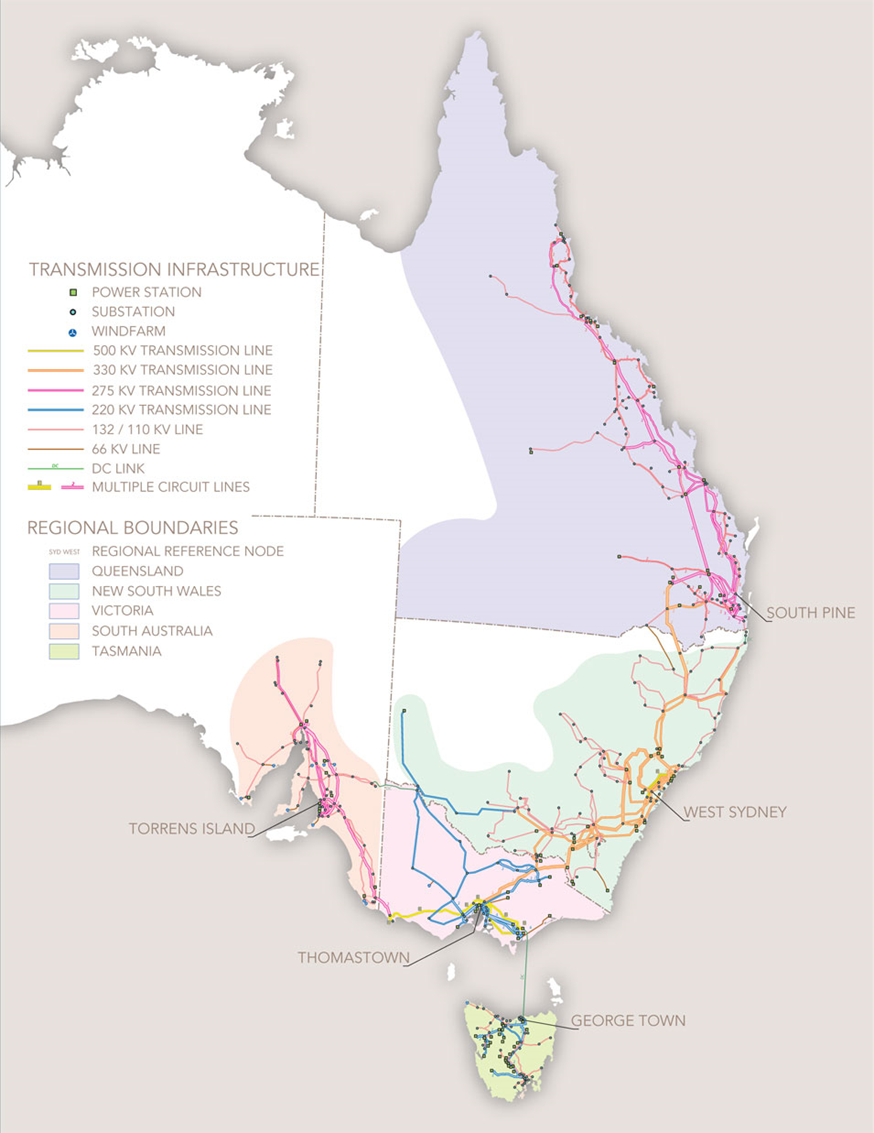
\includegraphics[width=0.8\textwidth,height=\textheight]{source/figures/NEM.png}
\caption[The National Electricity Market (NEM)]{Regions/states and
transmission in the NEM. Source: Australian Energy Market Commission
(\protect\hyperlink{ref-australianenergymarketcommissionNationalElectricityMarket}{n.d.a})}\label{fig:NEM}
}
\end{figure}

The NEM is a single platform (real-time) energy-only market with no
explicit capacity mechanisms. Unit commitment is managed by market
participants, who must submit resource-specific offers for energy and
Frequency Control Ancillary Services (FCAS) capacity in price-quantity
pairs the day before delivery. These offers are subsequently used in a
pre-dispatch process, which provides forecasted market information
(e.g.~generation and demand, interconnector flows, prices, etc.) to
market participants. While prices in submitted offers are fixed,
participants may change the energy volumes in their offer up to a few
minutes before the delivery dispatch interval commences. As the NEM is
single-sided, security-constrained economic dispatch is run every five
minute to meet forecast demand at least cost, subject to network and
security constraints. Much like ISO/RTO markets, energy and FCAS markets
are co-optimised with respect to technical feasibility and cost
(\protect\hyperlink{ref-australianenergymarketoperatorDispatchStandardOperating2019}{Australian
Energy Market Operator, 2021d},
\protect\hyperlink{ref-australianenergymarketoperatorFCASModelNEMDE2017}{2017b}).
Real-time dispatch produces zonal marginal prices for energy and FCAS,
which form the basis for market settlement in each of the NEM's regions.

\hypertarget{fcas-markets}{%
\subsection{FCAS markets}\label{fcas-markets}}

The NEM's competitive FCAS markets consist of eight separate raise and
lower FCAS products that can be classed as regulation FCAS or
contingency FCAS, with the former responsible for control when frequency
is within the normal operating frequency band (NOFB) and the latter for
when frequency deviates outside the NOFB after an event (see
Table~\ref{tbl:fcs-fcas}). This is similar to arrangements in many
ISO/RTO markets, where FCS are divided into event and non-event reserves
(\protect\hyperlink{ref-elaOperatingReservesVariable2011}{Ela et al.,
2011}).

Security-constrained economic dispatch includes system-wide and regional
FCAS requirement constraints. Regulation and contingency FCAS are
typically procured for and from all regions of the NEM in the absence of
binding local constraints. Local requirements for FCAS procurement apply
to Tasmania and to the other regions of the NEM if they experience
network constraints, are at risk of separation or when
islanded\footnote{From 2015-2019, the Tasmanian and mainland contingency
  FCAS markets were separated on average for 40\% of the time due to the
  technical limitations of the high voltage DC interconnector
  (\protect\hyperlink{ref-ghdadvisoryGHDReportTasNetworks2019}{GHD
  Advisory, 2019}). However, if the interconnector flow is within the
  appropriate operating envelope, NEM-wide FCAS procurement is possible
  as the interconnector's frequency controller enables FCAS transfer
  between the mainland and Tasmania
  (\protect\hyperlink{ref-australianenergymarketoperatorInterconnectorCapabilitiesNational2017}{Australian
  Energy Market Operator, 2017c}).}
(\protect\hyperlink{ref-australianenergymarketoperatorConstraintImplementationGuidelines2015}{Australian
Energy Market Operator, 2015a},
\protect\hyperlink{ref-australianenergymarketoperatorConstraintFormulationGuidelines2010}{2010}).
Prices are calculated for each region of the NEM based on the sum of the
shadow prices of local and system-wide constraints and FCAS costs are
allocated to market participants based on a "Causer Pays" principle,
which bears similarities to imbalance penalties in European markets
(\protect\hyperlink{ref-australianenergymarketoperatorGuideAncillaryServices2015}{Australian
Energy Market Operator, 2015b}). FCAS providers are paid for enablement
(capacity provision) regardless of whether their capacity is activated
(\protect\hyperlink{ref-australianenergymarketoperatorGuideAncillaryServices2015}{Australian
Energy Market Operator, 2015b};
\protect\hyperlink{ref-rieszFrequencyControlAncillary2015}{Riesz et al.,
2015};
\protect\hyperlink{ref-thorncraftExperienceMarketbasedAncillary2007}{Thorncraft
and Outhred, 2007}).

For a resource to provide FCAS, it must meet pre-qualification criteria
and undergo a registration process. Historically, FCAS was provided by
thermal generation (predominantly coal and some gas), hydropower
generation and some large loads, such as hydropower pumps and an
aluminium smelter, as only resources associated with wholesale energy
market participants were permitted to offer FCAS. In 2017, the first
battery energy storage system (BESS) in the NEM began to offer FCAS and
market reform enabled demand response (DR) aggregators to offer
contingency FCAS without participating in the energy market
(\protect\hyperlink{ref-aureconLargeScaleBatteryStorage2019}{Aurecon,
2019};
\protect\hyperlink{ref-australianenergymarketcommissionNationalElectricityAmendment2016}{Australian
Energy Market Commission, 2016}). In recent years, new FCAS market
entrants have included several DR aggregators, new BESS, distributed
PV-battery virtual power plants and wind farms (the latter two through
trials)
(\protect\hyperlink{ref-aureconLargeScaleBatteryStorage2019}{Aurecon,
2019};
\protect\hyperlink{ref-australianenergymarketoperatorAEMOVirtualPower2021}{Australian
Energy Market Operator, 2021e};
\protect\hyperlink{ref-australianenergyregulatorStateEnergyMarket2021}{Australian
Energy Regulator, 2021}). However, these new entrants tend to offer
smaller volumes and there are still relatively few FCAS providers in the
NEM, with no single FCAS product having more than 30 providers across
the system or 8 providers in any one region
(\protect\hyperlink{ref-australianenergyregulatorStateEnergyMarket2021}{Australian
Energy Regulator, 2021}).

\blandscape

\def\pandoctableshortcapt{Frequency control ancillary services in the
NEM}

\hypertarget{tbl:fcs-fcas}{}
\begin{longtable}[]{@{}
  >{\raggedright\arraybackslash}m{(\columnwidth - 6\tabcolsep) * \real{0.2182}}
  >{\raggedright\arraybackslash}m{(\columnwidth - 6\tabcolsep) * \real{0.2606}}
  >{\raggedright\arraybackslash}m{(\columnwidth - 6\tabcolsep) * \real{0.2667}}
  >{\raggedright\arraybackslash}m{(\columnwidth - 6\tabcolsep) * \real{0.2424}}@{}}
\caption[Frequency control ancillary services in the
NEM]{\label{tbl:fcs-fcas}Frequency control ancillary services in the
National Electricity Market. Sources: Thorncraft and Outhred
(\protect\hyperlink{ref-thorncraftExperienceMarketbasedAncillary2007}{2007}),
Riesz et al.
(\protect\hyperlink{ref-rieszFrequencyControlAncillary2015}{2015}),
Australian Energy Market Operator
(\protect\hyperlink{ref-australianenergymarketoperatorFastFrequencyResponse2017}{2017a}),
Australian Energy Market Operator
(\protect\hyperlink{ref-australianenergymarketoperatorConstraintFormulationGuidelines2010}{2010}),
Australian Energy Market Operator
(\protect\hyperlink{ref-australianenergymarketoperatorConstraintImplementationGuidelines2015}{2015a}),
Australian Energy Market Operator
(\protect\hyperlink{ref-australianenergymarketoperatorGuideAncillaryServices2015}{2015b}),
Australian Energy Market Operator
(\protect\hyperlink{ref-australianenergymarketoperatorPowerSystemRequirements2020}{2020b}).}\tabularnewline
\toprule\noalign{}
\begin{minipage}[b]{\linewidth}\raggedright
Product
\end{minipage} & \begin{minipage}[b]{\linewidth}\raggedright
Control action
\end{minipage} & \begin{minipage}[b]{\linewidth}\raggedright
Procurement
\end{minipage} & \begin{minipage}[b]{\linewidth}\raggedright
Timeframe
\end{minipage} \\
\midrule\noalign{}
\endfirsthead
\toprule\noalign{}
\begin{minipage}[b]{\linewidth}\raggedright
Product
\end{minipage} & \begin{minipage}[b]{\linewidth}\raggedright
Control action
\end{minipage} & \begin{minipage}[b]{\linewidth}\raggedright
Procurement
\end{minipage} & \begin{minipage}[b]{\linewidth}\raggedright
Timeframe
\end{minipage} \\
\midrule\noalign{}
\endhead
\bottomrule\noalign{}
\endlastfoot
Regulation (raise \& lower) & Centralised control through AEMO Automatic
Generation Control (AGC), which adjusts unit set points & Minimum
capacity enablement with dynamic additional reserve setting based on
time error for every dispatch interval & Unit set points adjusted by AGC
every 4-s over dispatch interval \\
6-s contingency (fast raise \& lower) & \multirow{2}{=}{Decentralised
control response to locally-measured frequency, typically delivered
through droop settings in governors or inverters or frequency-responsive
loads (raise only)} & \multirow{2}{=}{Capacity enablement based on size
of largest generator (raise) or load block (lower), minus assumed load
relief for every dispatch interval} & Full response delivered by 6-s
after frequency has left NOFB and orderly transition to 60-s service \\
60-s contingency (slow raise \& lower) & & & Full response delivered by
60-s after frequency has left NOFB and orderly transition to 5-min
service \\
5-min contingency (delayed raise \& lower) & Response pre-configured by
AEMO but triggered in response to locally-measured frequency. Typically
consists of unit control systems increasing or decreasing set points
with sustained frequency deviations & Capacity enablement based on size
of largest generator (raise) or load block (lower), minus assumed load
relief and corresponding Regulation FCAS procurement for every dispatch
interval & Full response delivered by 5-min after frequency has left
NOFB and sustained until frequency returns to NOFB or 10-min has
elapsed \\
\end{longtable}

\let\pandoctableshortcapt\relax

\elandscape

\hypertarget{nem-operation-and-governance}{%
\subsection{NEM operation and
governance}\label{nem-operation-and-governance}}

The Australian Energy Market Operator (AEMO) is responsible for the
operation of the market and power system in the NEM in accordance with
the National Electricity Rules (NER). They act as a single buyer of
dynamically-determined volumes of FCS. The Australian Energy Market
Commission (AEMC) is responsible for making or amending rules for the
NEM. Both AEMO and the AEMC provide operational and strategic advice to
the Energy Security Board (ESB), which is responsible for coordinating
market oversight and longer-term reform such as the ongoing post-2025
NEM market design framework. As the market regulator, the Australian
Energy Regulator (AER) monitors compliance with and enforces the NER.

\hypertarget{challenges-to-frequency-control-posed-by-vre-and-ibr}{%
\subsection{Challenges to frequency control posed by VRE and
IBR}\label{challenges-to-frequency-control-posed-by-vre-and-ibr}}

The rapid pace at which IBR have entered the NEM was preceded by the
exit of FCAS-capable synchronous generation
(Figure~\ref{fig:entry_exit}). Many of these IBR do not currently offer
FCAS or any meaningful frequency response to deviations other than the
most extreme. Furthermore, though updated equipment standards require
distributed IBR to ride-through and/or respond to certain frequency
deviations, some inverter models have been found to be non-compliant and
there is still a significant number of legacy systems in the NEM
(\protect\hyperlink{ref-australianenergymarketoperatorBehaviourDistributedResources2021}{Australian
Energy Market Operator, 2021f};
\protect\hyperlink{ref-stringerConsumerLedTransitionAustralia2020}{Stringer
et al., 2020}).

\begin{figure}
\hypertarget{fig:entry_exit}{%
\centering
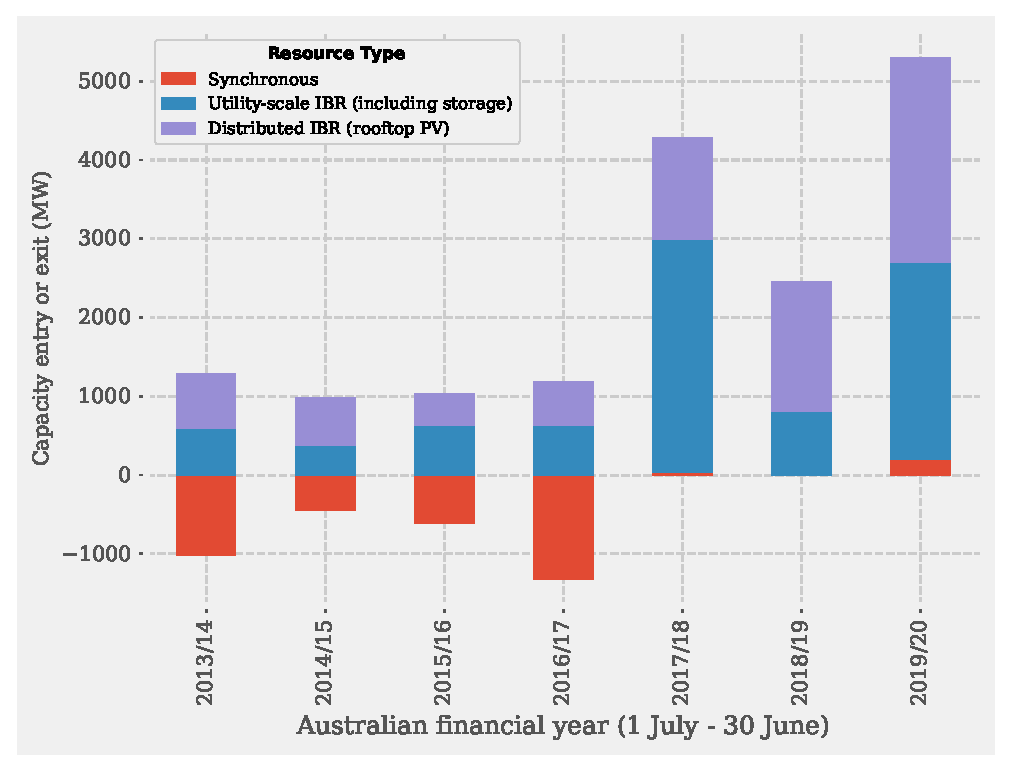
\includegraphics{source/figures/synchronous_ibr_entry_exit.eps}
\caption[Entry and exit of generation capacity in the NEM between
2013/14 and 2019/20]{Entry (of IBR) and exit (of synchronous generation)
capacity in the NEM between Australian financial years 2013/14 and
2019/20. Data source: Australian Energy Market Commission
(\protect\hyperlink{ref-australianenergymarketcommissionAnnualMarketPerformance2020}{2020a}).}\label{fig:entry_exit}
}
\end{figure}

The challenges that VRE and other IBR pose to frequency control have
been exacerbated by the NEM's network topology. Limited interconnection
between regions reduces the NEM's cross-regional balancing capabilities
and increases the likelihood of synchronous area separation following
power system events, a consequence of which is that local requirements
for FCAS may apply
(\protect\hyperlink{ref-australianenergymarketoperatorMaintainingPowerSystem2019}{Australian
Energy Market Operator, 2019a}). Furthermore, correlated variability and
uncertainty can arise from intensive development of similar
utility-scale VRE in areas with good wind or solar resources (as might
occur in the Renewable Energy Zones identified by AEMO's least-regrets
transmission planning study
(\protect\hyperlink{ref-australianenergymarketoperator2020IntegratedSystem2020}{Australian
Energy Market Operator, 2020f})). This is also an issue at the
distribution level given the significant installed capacities of rooftop
solar PV located within proximity of one another in suburban areas
(\protect\hyperlink{ref-australianenergymarketoperatorEnduringPrimaryFrequency2021}{Australian
Energy Market Operator, 2021a}).

\hypertarget{features-of-nem-frequency-control-arrangements}{%
\subsection{Features of NEM frequency control
arrangements}\label{features-of-nem-frequency-control-arrangements}}

Below, we highlight some noteworthy features of the NEM's frequency
control arrangements that complement or contrast previous analyses in
Thorncraft and Outhred
(\protect\hyperlink{ref-thorncraftExperienceMarketbasedAncillary2007}{2007}),
Riesz et al.
(\protect\hyperlink{ref-rieszFrequencyControlAncillary2015}{2015}) and
Thorncraft et al.
(\protect\hyperlink{ref-thorncraftMarketbasedAncillaryServices2008}{2008}).

\hypertarget{control-mechanisms}{%
\subsubsection{Control mechanisms:}\label{control-mechanisms}}

\begin{itemize}
\tightlist
\item
  There is no explicit TFR FCS in the NEM. Security-constrained economic
  dispatch is run every five minutes and is expected to relieve PFR and
  SFR and address supply-demand imbalances
  (\protect\hyperlink{ref-australianenergymarketoperatorPowerSystemRequirements2020}{Australian
  Energy Market Operator, 2020b}).
\item
  PFR from contingency FCAS is only required to respond to frequency
  deviations outside the NOFB (50 \(\pm\) 0.15 Hz). When FCAS markets
  were implemented in the NEM in 2001, mandatory PFR around a tight
  deadband of \(\pm\) 50 mHz was removed from the NER
  (\protect\hyperlink{ref-australianenergymarketoperatorElectricityRuleChange2019}{Australian
  Energy Market Operator, 2019b}). Since then and prior to 2020, there
  was no explicit procurement or requirement for tight-deadband PFR
  provision within the NOFB. The decline in the provision of
  tight-deadband PFR in the NEM is discussed further in
  Section~\ref{sec:fcs-pfr}.
\item
  The mainland synchronous area is controlled as one balancing area by
  AEMO's AGC (i.e.~no tie-line biased SFR) despite limited
  interconnection between adjacent regions
  (\protect\hyperlink{ref-australianenergymarketoperatorAEMCFrequencyControl2018}{Australian
  Energy Market Operator, 2018a}). AGC control performance is discussed
  further in Section~\ref{sec:fcs-regulation}.
\end{itemize}

\hypertarget{market-based-mechanisms}{%
\subsubsection{Market-based mechanisms:}\label{market-based-mechanisms}}

\begin{itemize}
\tightlist
\item
  There are relatively few limits imposed on FCAS participation. FCAS
  can be provided by any technology through variable, switched or hybrid
  controllers
  (\protect\hyperlink{ref-australianenergymarketoperatorMarketAncillaryService2020a}{Australian
  Energy Market Operator, 2020g}). Furthermore, regulation and
  contingency FCAS products are unbundled into raise and lower services,
  and contingency FCAS products are unbundled based on response time.
  All of these features improve the potential for participation and
  competition in FCAS markets, though market participants can and often
  are enabled to provide multiple FCAS.
\item
  FCAS unbundling has enabled a `Causer Pays' cost allocation framework.
  Raise contingency FCAS costs, which are incurred as insurance for the
  failure of a generator, are distributed amongst generators in
  proportion to their generation in the trading interval. Similarly,
  lower contingency FCAS costs are distributed amongst loads based on
  their consumption in a trading interval. A complex methodology is used
  to calculate monthly, portfolio-wide Causer Pays contribution factors
  (outlined in Australian Energy Market Operator
  (\protect\hyperlink{ref-australianenergymarketoperatorRegulationFCASContribution2018a}{2018b})
  and summarised in Riesz et al.
  (\protect\hyperlink{ref-rieszFrequencyControlAncillary2015}{2015}))
  that determine how regulation FCAS costs are allocated to market
  participants. We discuss the issues associated with this methodology
  in Section~\ref{sec:fcs-regulation}.
\item
  The NEM co-optimises FCAS that respond within similar timeframes. In
  the absence of constraints, the volume of 5-minute delayed contingency
  FCAS procured is reduced by the volume of regulation FCAS enabled
  (\protect\hyperlink{ref-australianenergymarketoperatorConstraintFormulationGuidelines2010}{Australian
  Energy Market Operator, 2010}).
\end{itemize}

\hypertarget{regulatory-mechanisms}{%
\subsubsection{Regulatory mechanisms:}\label{regulatory-mechanisms}}

\begin{itemize}
\item
  Connecting utility-scale generators negotiate the frequency response
  capability of their plant between a minimum access standard and an
  automatic access standard, the latter guaranteeing network access to
  the applicant. A suite of generator standards for frequency response
  were added to the NER in October 2018 and apply to any
  newly-connecting generation. These standards include minimum frequency
  disturbance ride-through times, automatic generation output reduction
  following extreme over-frequency events and the capability to operate
  in a frequency response mode with a proportional response\footnote{In
    addition to these standards, newly-connected generation may install
    a synchronous condenser under the `do no harm' requirements outlined
    in the NER if they are determined to have an adverse impact on
    system strength. Particularly when fitted with a rotating mass or
    flywheel, these synchronous condensers can also provide inertial
    response
    (\protect\hyperlink{ref-australianenergymarketoperatorSystemStrengthNEM2020}{Australian
    Energy Market Operator, 2020h}).}
  (\protect\hyperlink{ref-australianenergymarketcommissionGeneratorTechnicalPerformance2018}{Australian
  Energy Market Commission, 2018a}).
\item
  Transmission Network Service Providers (TNSPs) are required to address
  any inertia shortfalls identified by AEMO within the NEM region in
  which they build, maintain, plan and operate the transmission network.
  AEMO's assessment considers whether an islanded region can be securely
  operated following a contingency event. Shortfalls can be reduced by
  special protection schemes (e.g.~disconnection of load following
  interconnector trip) and the provision of FFR, but they must
  ultimately be met by providers of inertial response
  (\protect\hyperlink{ref-australianenergymarketoperatorNoticeSouthAustralia2020}{Australian
  Energy Market Operator, 2020i},
  \protect\hyperlink{ref-australianenergymarketoperatorInertiaRequirementsMethodology2018}{2018c}).
\end{itemize}

\hypertarget{sec:fcs-insights}{%
\section{Insights from the National Electricity
Market}\label{sec:fcs-insights}}

In light of existing challenges and those posed by energy transition,
effective and efficient frequency control arrangements should enable
sufficient FCS to be procured across timeframes and strike the
appropriate balance between efficiency and robustness. In the following
sections, we review issues associated with two core elements of the
NEM's frequency control hierarchy (i.e.~PFR and SFR), assess their
physical and economic performance and outline reform underway. Drawing
on developments in the NEM and our review of arrangements in North
America and Europe, we then discuss the merits and flaws of regulatory
and market-based mechanisms with respect to sufficiency and efficiency.
We conclude by offering insights that could serve as design principles
for jurisdictions revisiting their frequency control arrangements during
energy transition.

\hypertarget{sec:fcs-pfr}{%
\subsection{Declining tight-deadband primary frequency
response}\label{sec:fcs-pfr}}

When FCAS markets were implemented in 2001, mandatory tight-deadband PFR
was superseded by two types of PFR: voluntary PFR within the NOFB and
competitive procurement for PFR outside the NOFB in the form of
contingency FCAS
(\protect\hyperlink{ref-australianenergymarketoperatorElectricityRuleChange2019}{Australian
Energy Market Operator, 2019b}).

As such, the NEM's frequency control scheme deviated from what has been
argued to be international best practice as it only explicitly specified
and procured wide-deadband PFR (i.e.~deadband of \(\pm\) 150 mHz)
(\protect\hyperlink{ref-australianenergymarketoperatorElectricityRuleChange2019}{Australian
Energy Market Operator, 2019b}). In contrast, ENTSO-E specifies that PFR
providers have a deadband no greater than \(\pm\) 10-15 mHz depending on
the control area
(\protect\hyperlink{ref-europeannetworkoftransmissionsystemoperatorsforelectricityentso-eNetworkCodeLoadFrequency2013}{European
Network of Transmission System Operators for Electricity, 2013}) and
FERC Order 842 mandates all newly-connecting generation in US
interconnections to operate frequency-responsive control equipment with
maximum deadbands of \(\pm\) 36 mHz
(\protect\hyperlink{ref-federalenergyregulatorycommissionfercOrderNo8422018}{Federal
Energy Regulatory Commission, 2018a}).

In recent years in the NEM, the lack of an incentive or requirement for
tight-deadband PFR and perceived disincentives to its provision (through
Causer Pays contribution factors discussed further in
Section~\ref{sec:fcs-regulation}) has led to many synchronous generators
that once provided tight-deadband PFR to widen deadbands or install
control systems that block or dampen PFR from the speed governor within
the NOFB
(\protect\hyperlink{ref-australianenergymarketcommissionMandatoryPrimaryFrequency2020}{Australian
Energy Market Commission, 2020b}). Furthermore, many VRE generators were
deployed in the NEM and connected with inverter control systems that
were unresponsive to any frequency deviations other than the most
serious.

The extent to which tight-deadband PFR provision had declined in the NEM
and the consequences of this became clear to AEMO following a major
power system incident on the 25\textsuperscript{th} of August 2018
(\protect\hyperlink{ref-australianenergymarketoperatorFinalReportQueensland2019}{Australian
Energy Market Operator, 2019c}). Prior to the event, the QLD region was
exporting \(\sim\) 900 MW to the rest of the NEM. Around 13:11:41,
lightning strikes at the QLD-NSW interconnector resulted in the QLD
region being separated from the rest of the NEM with excess supply. The
SA region was exporting \(\sim\) 200 MW prior to the event and following
QLD's separation, this increased by more than 200 MW in response to
under-frequency. The sudden increase in active power flow triggered an
emergency scheme that disconnected SA from the NSW-VIC synchronous area,
resulting in local over-frequency.

There were diverse responses from various generators following the
double separation event. While many synchronous generators provided some
form of PFR though not enabled for FCAS, their response was withdrawn by
their load controllers in several cases so that the unit could return to
its dispatch target (e.g.~green and pink lines in top frame of
Figure~\ref{fig:plant_responses}). Wind and solar farms were either
unresponsive, tripped due to protection settings in their inverters, or
reduced their active power output in line with performance standards
negotiated in their connection agreements (middle and bottom frames in
Figure~\ref{fig:plant_responses}). AEMO attributed slow frequency
recovery and under-frequency load shedding in NSW and VIC to
insufficient PFR from generators and a lack of appropriate contingency
FCAS within the islanded regions. Over 50\% of fast and slow raise
contingency FCAS needed in NSW-VIC was enabled in SA and QLD, whilst QLD
had no lower FCAS enabled to respond to over-frequency\footnote{AEMO is
  currently investigating appropriate regional requirements for FCAS,
  particularly for contingency FCAS in the terminal regions of QLD and
  SA
  (\protect\hyperlink{ref-australianenergymarketoperatorRenewableIntegrationStudy2020b}{Australian
  Energy Market Operator, 2020j},
  \protect\hyperlink{ref-australianenergymarketoperatorElectricityRuleChange2019a}{2019d}).}
(\protect\hyperlink{ref-australianenergymarketoperatorFinalReportQueensland2019}{Australian
Energy Market Operator, 2019c}).

\begin{figure}
\hypertarget{fig:plant_responses}{%
\centering
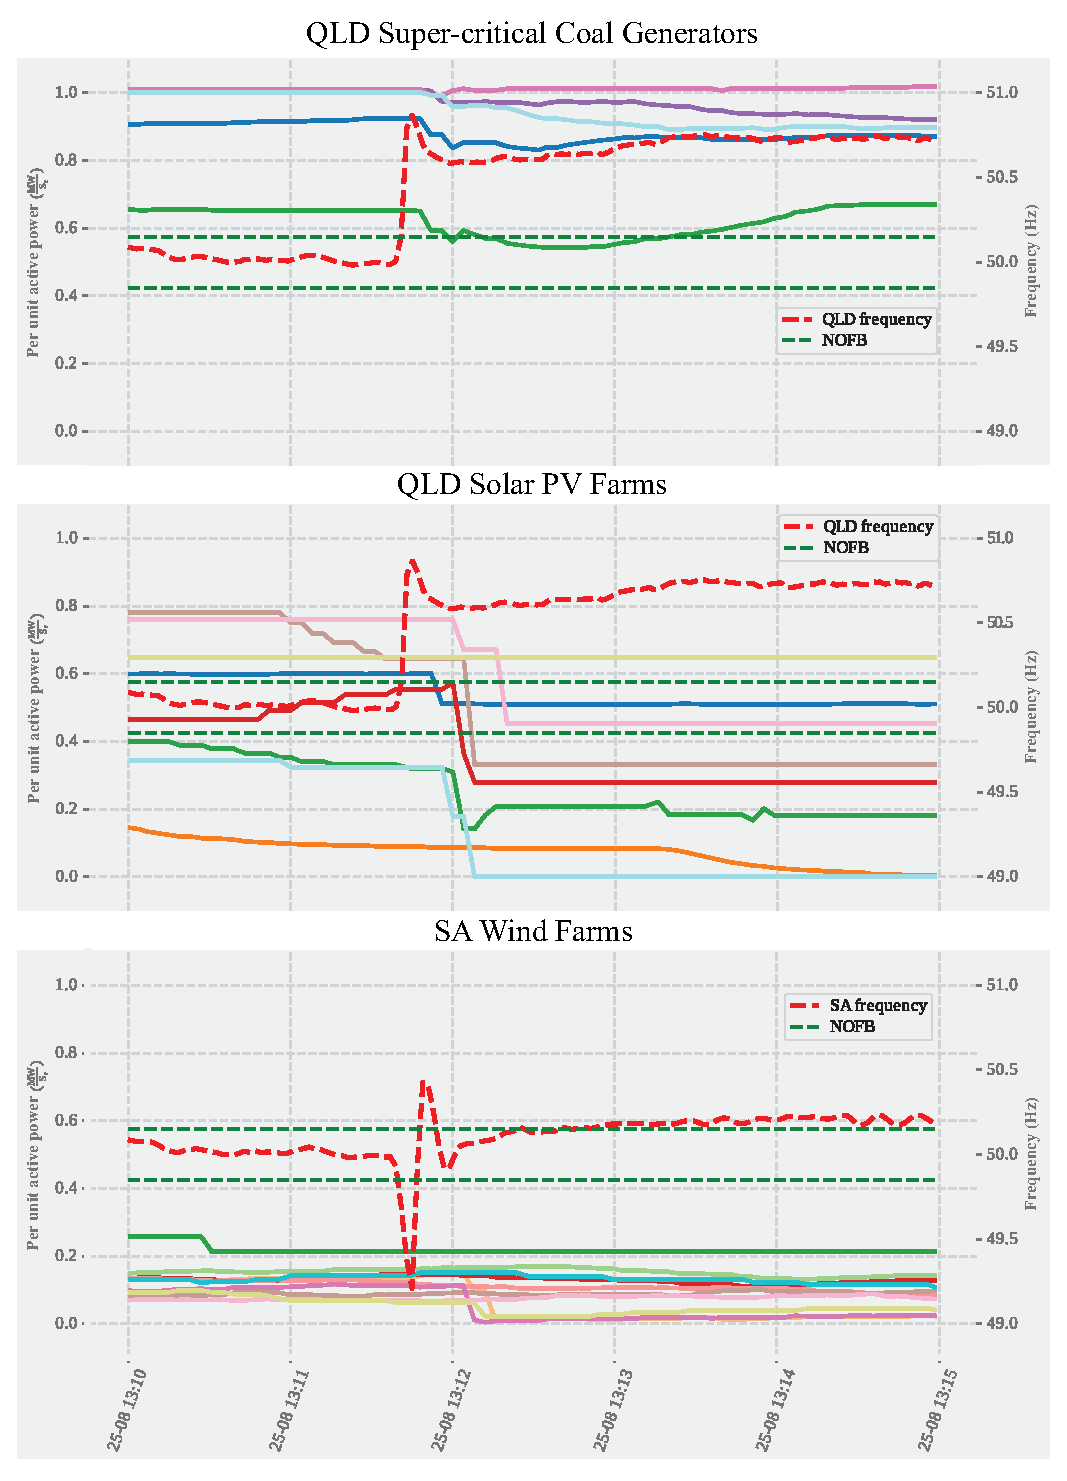
\includegraphics{source/figures/all_responses_25082018.eps}
\caption[Response of different generation technologies to power system
events on the 25th of August, 2018]{Active power output of QLD
super-critical coal generators (top), SA solar PV farms (middle) and SA
wind farms (bottom). The response of an individual generator is denoted
by solid lines (obtained from 4-second AEMO SCADA data using NEMOSIS
(\protect\hyperlink{ref-gormanNEMOSISNEMOpen2018}{Gorman et al.,
2018})). None of these generators are enabled for FCAS. The red dashed
line in each frame is the regional frequency as measured by high-speed
(1-second) phasor measurement units.}\label{fig:plant_responses}
}
\end{figure}

Prior to this incident, deteriorating control of frequency within the
NOFB was of concern to AEMO and the AEMC, and trials and investigations
were recommended to inform the design of an incentive for tight-deadband
PFR provision
(\protect\hyperlink{ref-australianenergymarketcommissionFrequencyControlFrameworks2018}{Australian
Energy Market Commission, 2018b}). However, this separation event
demonstrated the ``urgent need for regulatory changes to arrest the
ongoing decline in frequency performance in the NEM'' and to enhance
``the resilience of the NEM to similar major disturbances'', with AEMO
submitting a rule change proposal for all capable generators in the NEM
to provide mandatory PFR with a maximum deadband of \(\pm\) 0.015 Hz
(i.e.~10\% of the NOFB)
(\protect\hyperlink{ref-australianenergymarketoperatorElectricityRuleChange2019}{Australian
Energy Market Operator, 2019b}).

This rule was initially incorporated into the NER in 2020 as a temporary
arrangement through the addition of a ``sunset'' after three years to
demonstrate the AEMC's commitment to investigating incentives or
market-based mechanisms for tight-deadband PFR
(\protect\hyperlink{ref-australianenergymarketcommissionMandatoryPrimaryFrequency2020}{Australian
Energy Market Commission, 2020b},
\protect\hyperlink{ref-australianenergymarketcommissionFrequencyControlRule2020}{2020c}).
AEMO has specified PFR settings, including maximum droop and response
time, but is unable to require generation to reserve headroom for PFR
(\protect\hyperlink{ref-australianenergymarketoperatorInterimPrimaryFrequency2020}{Australian
Energy Market Operator, 2020k}).

\hypertarget{sec:fcs-regulation}{%
\subsection{Performance and efficiency issues of regulation
services}\label{sec:fcs-regulation}}

For SFR provided by regulation FCAS within the NOFB to be effective, the
dynamics of the system need to accommodate slower SFR control action and
the centralised secondary controller (in the NEM, AEMO's AGC) needs to
be properly configured. Prior to the introduction of mandatory PFR in
the NEM, AEMO observed no significant improvement in NOFB frequency
stability despite several increases in the minimum volumes procured for
regulation FCAS in 2019
(\protect\hyperlink{ref-australianenergymarketoperatorElectricityRuleChange2019}{Australian
Energy Market Operator, 2019b}). This is likely due to:

\begin{itemize}
\tightlist
\item
  A lack of fast and decentralised tight-deadband PFR supporting slower
  SFR;
\item
  Inappropriate control signals being calculated within the AGC due to
  the use of rate limiters to account for ramping constraints, signal
  filtering and generator controller models that do not accurately
  reflect a unit's frequency response
  (\protect\hyperlink{ref-digsilentReviewFrequencyControl2017}{DIgSILENT,
  2017}). The latter is the consequence of an absence of control
  coordination between market participants and AEMO; and
\item
  Variable communication delays between individual unit controllers and
  AEMO's AGC system, and disparate response times from generators.
\end{itemize}

Furthermore, the control of all mainland regions as one balancing area
can be problematic in the event of separation. AGC control of regulation
FCAS enabled in islanded regions may exacerbate local frequency
deviations when responding to the AGC frequency reference. This was the
case during the double separation event on the 25\textsuperscript{th} of
August 2018, in which the AGC instructed raise regulation FCAS
generators in QLD and SA to respond to under-frequency in the AGC
frequency reference despite local over-frequency
(Figure~\ref{fig:regional_freq}). Such incorrect control action can
occur until AEMO is able to manually reconfigure the AGC to treat each
island as a control area - a process which can take up to 15 minutes
(\protect\hyperlink{ref-australianenergymarketoperatorFinalReportQueensland2019}{Australian
Energy Market Operator, 2019c}) .

\begin{figure}
\hypertarget{fig:regional_freq}{%
\centering
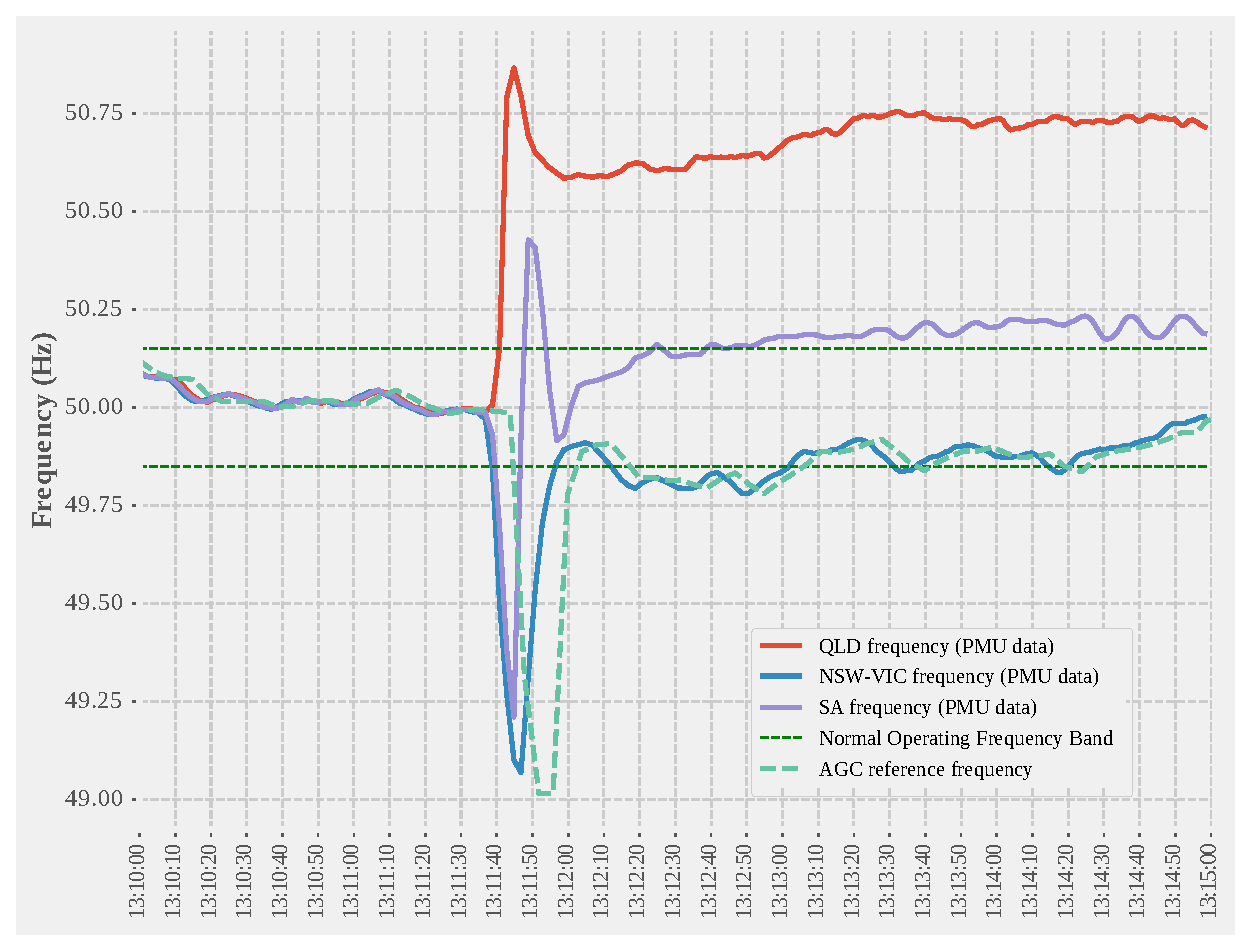
\includegraphics{source/figures/regional_SCADA_frequencies.eps}
\caption[System frequency (as registered by phasor measurement units and
AEMO\textquotesingle s AGC) during the power system event on the
25\^{}th\^{} of August, 2018]{Regional phasor measurement unit frequency
data and AGC reference frequency data from AEMO's NSW control centre
(obtained using NEMOSIS
(\protect\hyperlink{ref-gormanNEMOSISNEMOpen2018}{Gorman et al., 2018}))
during the power system event on the 25\textsuperscript{th} of August,
2018. Note that the AGC reference frequency deviates in the opposite
direction to local frequency in QLD and SA.}\label{fig:regional_freq}
}
\end{figure}

Over time, inefficiencies in regulation FCAS procurement and
cost-allocation have also become apparent. Regulation FCAS procurement
in the NEM is dynamic beyond a minimum volume, but the dynamic component
is based on the system time error
(\protect\hyperlink{ref-australianenergymarketoperatorConstraintImplementationGuidelines2015}{Australian
Energy Market Operator, 2015a}). Time error control is largely
unnecessary as modern clocks no longer rely on power system frequency to
keep the time
(\protect\hyperlink{ref-reboursFundamentalDesignIssues2007}{Y. Rebours
et al., 2007}). Furthermore, whilst AEMO is required to control the NEM
within certain time error limits, these have been relaxed in recent
years
(\protect\hyperlink{ref-australianenergymarketcommissionreliabilitypanelStageOneFinal2017}{Australian
Energy Market Commission Reliability Panel, 2017}). Given that time
error is no longer prioritised as a control objective, dynamic
regulation FCAS procurement based on better measures of sustained
frequency deviation (e.g.~mean absolute error as suggested by Riesz et
al. (\protect\hyperlink{ref-rieszFrequencyControlAncillary2015}{2015}))
and/or a modelled distribution of potential intra-dispatch ramp
uncertainty may be more suitable.

Regulation FCAS costs are allocated to market participants based on
their contribution factor, a calculation which represents the extent to
which the participant has contributed to the need for regulation FCAS
through a deviation from a dispatch trajectory. Though the calculation
methodology assigns weights to a generator or load's dispatch trajectory
deviation based on the AGC regulation direction and mileage requirement
every 4 seconds, the disincentive for dispatch deviation suffers from a
disconnect to causation. This is because the contribution factors of a
generator or load are averaged over a 5-minute dispatch interval, summed
over a 28-day period and then within a market participant's portfolio
(\protect\hyperlink{ref-australianenergymarketcommissionFrequencyControlFrameworks2018}{Australian
Energy Market Commission, 2018b};
\protect\hyperlink{ref-australianenergymarketoperatorRegulationFCASContribution2018a}{Australian
Energy Market Operator, 2018b};
\protect\hyperlink{ref-australianenergyregulatorIssuesPaperSemi2020}{Australian
Energy Regulator, 2020}).

Much like portfolio-based balancing in Europe, the aggregation of
contribution factors enables a market participant to offset antagonistic
deviations with assisting deviations (from the provision of
tight-deadband PFR) across its resources and time. However, the
complexity and opacity of the methodology and cost-allocation process
has contributed to the withdrawal of tight-deadband PFR in the NEM.
Several generators disabled governor response in the NOFB in the belief
that dispatch adherence alone will minimise Causer Pays liabilities
(\protect\hyperlink{ref-digsilentReviewFrequencyControl2017}{DIgSILENT,
2017}).

\hypertarget{nem-assessment-and-outlook}{%
\subsection{NEM assessment and
outlook}\label{nem-assessment-and-outlook}}

Though the introduction of competitive FCAS markets in 2001 initially
resulted in significantly lower FCAS prices in the NEM
(\protect\hyperlink{ref-rieszFrequencyControlAncillary2015}{Riesz et
al., 2015};
\protect\hyperlink{ref-thorncraftExperienceMarketbasedAncillary2007}{Thorncraft
and Outhred, 2007}), volume-weighted average FCAS prices, particularly
those for raise regulation and contingency services, have increased
relative to the volume-weighted average energy price since 2016
(Figure~\ref{fig:raise_fcas_vwap}). Furthermore, the increases in
minimum regulation FCAS volumes and reductions in assumed load relief in
2019 have raised the procured volumes of regulation and contingency
FCAS, respectively. Together, these factors have contributed to higher
NEM-wide FCAS costs
(\protect\hyperlink{ref-australianenergymarketoperatorReviewNEMLoad2019}{Australian
Energy Market Operator, 2019e}). While quarterly FCAS costs were less
than 1\% of quarterly total NEM costs in 2015, 50\% of all quarters from
2017 to 2020 had FCAS costs that were between 1-2\% of total NEM cost
(\protect\hyperlink{ref-australianenergyregulatorStateEnergyMarket2021}{Australian
Energy Regulator, 2021}).

\begin{figure}
\hypertarget{fig:raise_fcas_vwap}{%
\centering
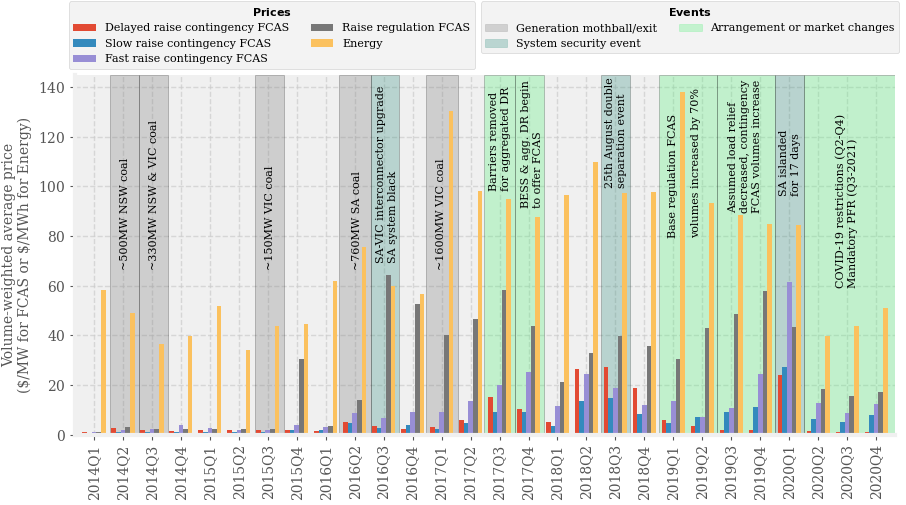
\includegraphics{source/figures/energy_raise_fcas_vwap_quarterly_2014_2020_v2.png}
\caption[Volume-weighted NEM-wide average quarterly prices for energy
and FCAS, 2014-2020]{Events and volume-weighted NEM-wide average
quarterly prices for energy, raise regulation FCAS and raise contingency
FCAS in the NEM. The entry of new albeit smaller FCAS providers in 2017
was preceded by the retirement of several large thermal generation. Q1
2020 FCAS prices were high due to local procurement in the SA region,
which was islanded for approximately two weeks. Note that while average
energy prices fell in Q2-Q4 in 2020 to levels previously seen in
2014-2015 (due to lower demand during COVID-19 lockdowns), FCAS prices
remained relatively high. Five-minute price and volume data obtained
using NEMOSIS (\protect\hyperlink{ref-gormanNEMOSISNEMOpen2018}{Gorman
et al., 2018}).}\label{fig:raise_fcas_vwap}
}
\end{figure}

Prior to the implementation of mandatory PFR, higher NEM FCAS costs were
arguably not accompanied by an improvement in frequency control
performance. Alongside deteriorating frequency control performance
within the NOFB (Figure~\ref{fig:nofb_freq_2005_2018}), AEMO has
expressed a loss of confidence in the NEM's resilience to complex power
system events, such as the double separation incident on the
25\textsuperscript{th} of August 2018
(\protect\hyperlink{ref-australianenergymarketoperatorElectricityRuleChange2019}{Australian
Energy Market Operator, 2019b}). These events are typically more severe
than the `credible' contingency events (i.e.~N-1 contingency) that
dictate the volume of contingency FCAS procured.

\begin{figure}
\hypertarget{fig:nofb_freq_2005_2018}{%
\centering
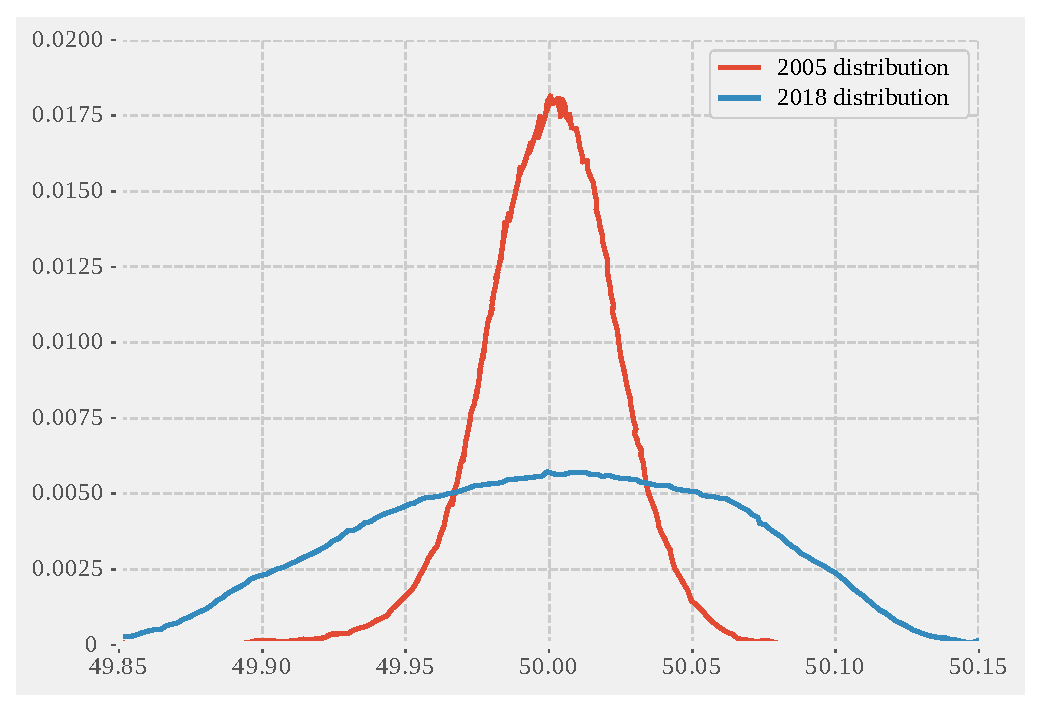
\includegraphics{source/figures/nem_nofb_frequency_2005_2018_digitised.eps}
\caption[NEM mainland frequency distributions, 2005 and 2018]{Normalised
distribution of mainland frequency within the NOFB in 2005 and 2018.
Reproduced from
(\protect\hyperlink{ref-australianenergymarketoperatorElectricityRuleChange2019a}{Australian
Energy Market Operator, 2019d})}\label{fig:nofb_freq_2005_2018}
}
\end{figure}

Since the implementation of the mandatory PFR, settings specified by
AEMO have been applied to a majority of large synchronous generators
(\(>\) 200MW) and some smaller synchronous generators. Despite the
absence of requirements for maintaining headroom and/or footroom,
preliminary analysis by AEMO\footnote{We note that AEMO has yet to
  complete mandatory PFR implementation. In particular, settings have
  yet to be changed for many VRE plant as inverter control system
  software changes are being trialled.} suggests that mandatory PFR has
delivered better control of frequency within the NOFB (see
Figure~\ref{fig:mpfr_dist}) and reduced excursions beyond the NOFB
(\protect\hyperlink{ref-australianenergymarketoperatorEnduringPrimaryFrequency2021}{Australian
Energy Market Operator, 2021a}). As a result of this initial success and
further technical advice provided by AEMO, the AEMC has indicated that
it intends to retain mandatory PFR at a tight-deadband following the
``sunset'' of the initial rule
(\protect\hyperlink{ref-australianenergymarketcommissionPrimaryFrequencyResponse2021}{Australian
Energy Market Commission, 2021a}).

\begin{figure}
\hypertarget{fig:mpfr_dist}{%
\centering
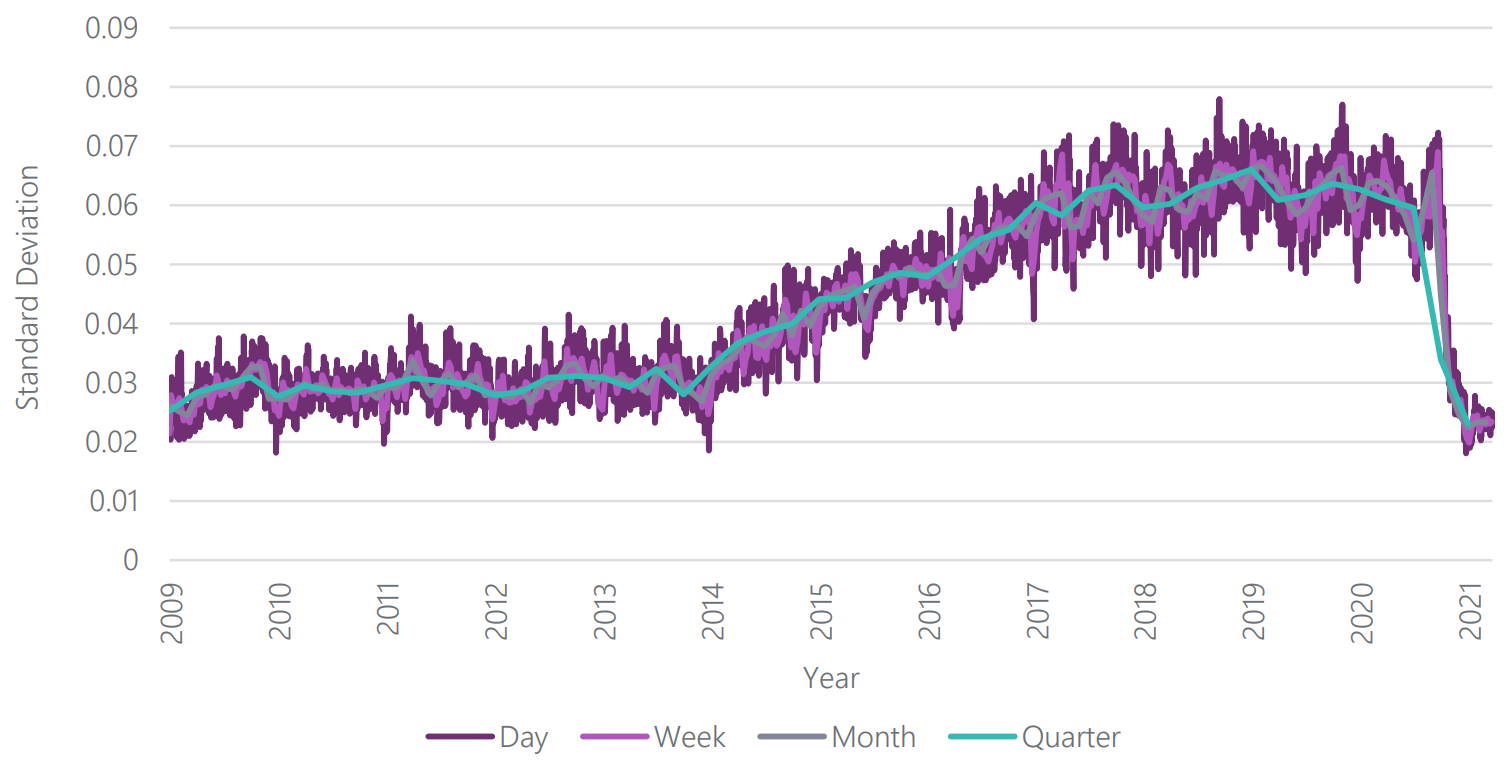
\includegraphics{source/figures/f_stddev_2009_2021.png}
\caption[Standard deviation of NEM mainland frequency from 2009 to
2021]{Standard deviation of mainland frequency grouped by each day,
week, month or quarter from 2009 to 2021. Some initial PFR setting
changes were made in late September 2020 and many generators moved to
final settings in late October 2020. Source: Australian Energy Market
Operator
(\protect\hyperlink{ref-australianenergymarketoperatorEnduringPrimaryFrequency2021}{2021a}).}\label{fig:mpfr_dist}
}
\end{figure}

However, this initial success may be a result of the headroom maintained
by these generators for risk management purposes (e.g.~defending
contract positions) and any headroom made available to the system
through the displacement of more expensive synchronous capacity by VRE.
Given that several large synchronous generators are expected to retire
in the coming decades
(\protect\hyperlink{ref-australianenergymarketoperator2020IntegratedSystem2020}{Australian
Energy Market Operator, 2020f}), continuing to rely on this ``free''
headroom (and any available footroom) into the future may reduce the
potential resilience benefits of widespread, tight-deadband PFR and
place a greater burden on generators that do reserve headroom and hence
respond. The AEMC is proposing to address this issue by paying resources
that provide assisting tight-deadband PFR (``double-siding'')
(\protect\hyperlink{ref-australianenergymarketcommissionPrimaryFrequencyResponse2021}{Australian
Energy Market Commission, 2021a}).

Presently, several other operational and market changes are being
considered or implemented with the goal of improving the effectiveness
of arrangements in the NEM. AEMO is investigating the use of dispatch
constraints to
(\protect\hyperlink{ref-australianenergymarketoperatorFrequencyControlWork2021}{Australian
Energy Market Operator, 2021g}):

\begin{itemize}
\tightlist
\item
  Procure contingency FCAS volumes based on system inertia;
\item
  Apply regional contingency and regulation FCAS requirements; and
\item
  To limit the amount of switched contingency FCAS procured. Switched
  FCAS has a number of limitations compared to governor-like control
  (\protect\hyperlink{ref-australianenergymarketoperatorRenewableIntegrationStudy2020c}{Australian
  Energy Market Operator, 2020e}).
\end{itemize}

These additional constraints will likely improve the effectiveness of
frequency control arrangements but may lead to higher FCAS costs. In
addition to these procurement changes, the AEMC has made a rule to
introduce raise and lower contingency markets for FFR by October 2023,
each with a likely response time of 1 second
(\protect\hyperlink{ref-australianenergymarketcommissionFastFrequencyResponse2021}{Australian
Energy Market Commission, 2021b};
\protect\hyperlink{ref-australianenergymarketoperatorFastFrequencyResponse2021}{Australian
Energy Market Operator, 2021h}). Whilst AEMO has highlighted that
potential stability issues and interconnector maloperation will need to
be managed (e.g.~through delivery caps or provision constraints)
(\protect\hyperlink{ref-australianenergymarketoperatorImplementationNationalElectricity2021}{Australian
Energy Market Operator, 2021i}), these FFR markets, along with the ESB's
proposals for short-term scheduling and/or procurement of inertial
response
(\protect\hyperlink{ref-energysecurityboardPost2025Market2021}{Energy
Security Board, 2021a}), will likely improve AEMO's operational toolbox
for managing a low-inertia NEM.

\hypertarget{reactive-regulatory-requirements}{%
\subsection{Reactive regulatory
requirements}\label{reactive-regulatory-requirements}}

Despite a broad set of FCS markets, there is a high degree of reliance
on regulatory mechanisms in the NEM. Performance standards and mandatory
PFR enforced by connection requirements in the NEM have recently been
aligned with international grid-codes
(\protect\hyperlink{ref-robertsReviewInternationalGrid2018}{Roberts,
2018}). As argued by TNSPs and AEMO during the mandatory PFR rule change
process, near-universal widespread provision of frequency control should
lead to relatively low costs for individual participants and be
outweighed by greater visibility and certainty for AEMO alongside the
system-wide benefits of improved physical frequency control performance
(\protect\hyperlink{ref-australianenergymarketoperatorElectricityRuleChange2019}{Australian
Energy Market Operator, 2019b};
\protect\hyperlink{ref-dillonMandatoryPrimaryFrequency2019}{Dillon,
2019};
\protect\hyperlink{ref-hopwoodMandatoryPrimaryFrequency2019}{Hopwood,
2019}).

Regulatory mechanisms are ideal for mandating basic FCS capabilities as
a condition for access, which may reduce the need to procure more
specialised FCS, or where FCS faces significant barriers to efficient
price formation or unbundled procurement. The latter reasons are
particularly pertinent in the NEM. Current FCAS prices do not appear to
be incentivising FCS provision from the vast majority of VRE generators,
which have business models centred around energy provision
(\protect\hyperlink{ref-australianenergymarketcommissionReserveServicesNational2021}{Australian
Energy Market Commission, 2021c};
\protect\hyperlink{ref-meegahapolaPowerSystemStability2021}{Meegahapola
et al., 2021}). Furthermore, procuring inertial response is challenging
due to its inseparability from system strength provision and unit
commitment costs
(\protect\hyperlink{ref-billimoriaMarketDesignSystem2020}{Billimoria et
al., 2020}). With respect to these challenges, regulatory mechanisms in
the NEM have assisted in ensuring some level of frequency response from
most power system resources (e.g.~mandatory PFR) and improving the
ability of AEMO and TNSPs to coordinate the procurement of essential but
``lumpy'' FCS (e.g.~inertia shortfall mechanism).

While mechanisms such as mandatory PFR are likely to improve the
robustness of frequency control arrangements, it may be difficult for
other regulatory mechanisms to keep in step with changing physical
performance requirements in systems rapidly facing higher penetrations
of VRE and IBR. Regulatory mechanisms are often only updated after a
number of years to reduce the burden placed on connecting resources. As
such, they are slow to respond to changing capabilities and
requirements. This delay often makes new standards and requirements
reactive rather than proactive. For example, AEMO can only review
utility-scale generator technical performance standards every 5 years
(\protect\hyperlink{ref-australianenergymarketcommissionGeneratorTechnicalPerformance2018}{Australian
Energy Market Commission, 2018a}), a timeframe in which the solar PV
capacity installed in the NEM has more than quadrupled (2015-2020)
(\protect\hyperlink{ref-australianpvinstituteInstalledPVGeneration}{Australian
PV Institute, n.d.}).

Additional concerns with regulatory mechanisms include poor dynamic
efficiency and opaque
costs(\protect\hyperlink{ref-rieszFrequencyControlAncillary2015}{Riesz
et al., 2015}). In the absence of remuneration or incentives,
particularly those that are linked to the quality of frequency response,
there is no incentive to innovate or invest in higher-quality frequency
control capabilities
(\protect\hyperlink{ref-meegahapolaPowerSystemStability2021}{Meegahapola
et al., 2021}). Furthermore, cost opacity may lead to FCS provision
costs being internalised within other prices (e.g.~energy) by
participants and prevent the implementation of imbalance or dispatch
non-conformance disincentives through cost-allocation mechanisms.

\hypertarget{preference-for-market-based-arrangements}{%
\subsection{Preference for market-based
arrangements}\label{preference-for-market-based-arrangements}}

Since the establishment of the NEM, a competition norm has been
established, with markets being viewed as a key driver for delivering
the National Electricity Objective of ``efficient investment in, and
efficient operation and use of electricity services''
(\protect\hyperlink{ref-hainesEnvironmentalNormsElectricity2016}{Haines
and McConnell, 2016};
\protect\hyperlink{ref-macgillElectricityMarketNorms2020}{MacGill et
al., 2020a}). This norm has pervaded all levels of participation and
governance in the NEM. Generator owners opposed the mandatory nature of
the mandatory PFR rule change on the basis that a lack of remuneration
was against market principles and that it would lead to economically
inefficient outcomes
(\protect\hyperlink{ref-rolfeMandatoryPrimaryFrequency2019}{Rolfe,
2019}; \protect\hyperlink{ref-scottMandatoryPrimaryFrequency2019}{Scott,
2019};
\protect\hyperlink{ref-skinnerMandatoryPrimaryFrequency2019}{Skinner,
2019}). AEMO did not include a headroom requirement in its proposal,
making the mandatory PFR rule change more palatable to market bodies and
participants. The AEMC, who have expressed a clear preference for
market-based approaches
(\protect\hyperlink{ref-australianenergymarketcommissionFrequencyControlFrameworks2018}{Australian
Energy Market Commission, 2018b}), included a ``sunset'' clause in their
initial decision to implement mandatory PFR. Furthermore, a market for
FFR will be implemented in 2023 and the ESB's post-2025 market design
process is considering new system services markets for inertial response
and TFR
(\protect\hyperlink{ref-energysecurityboardPost2025Market2021}{Energy
Security Board, 2021a},
\protect\hyperlink{ref-energysecurityboardPost2025Market2020}{2020b}).

If incentives or remuneration are designed correctly, markets can drive
short-run efficiency. Where required, they can also support investment
in FCS capability and assist a power system in achieving dynamically
efficient frequency control arrangements. However, in some cases, simply
introducing new FCS markets may serve as `patchwork' solutions to
existing control deficiencies and market failures. These deficiencies
and failures could be partially addressed by improving FCS cost
allocation processes, verifying FCS performance and linking incentives
to higher quality provision.

As discussed in {[}Section~\ref{sec:fcs-context}), efficient Causer Pays
cost-allocation mechanisms in FCS markets could provide suitable
disincentives for dispatch non-conformance or imbalances. In the NEM,
the aggregation of regulation FCAS Causer Pays contribution factors over
time and a portfolio has resulted in a blunt frequency performance
market signal. The solution to this problem may not be as simple as
strengthening disincentives (e.g.~as proposed by Hirth and Ziegenhagen
(\protect\hyperlink{ref-hirthBalancingPowerVariable2015}{2015}) and
Papavasiliou
(\protect\hyperlink{ref-papavasiliouScarcityPricingMissing2020}{2020}))
for resource-based cost-allocation processes as potential exposure to
high instantaneous FCS costs may lead to participants curtailing or
decommitting flexible resources rather than providing an assisting
frequency response. This has been observed in the NEM when local
constraints have resulted in regulation FCAS
(\protect\hyperlink{ref-australianenergymarketcommissionFrequencyControlFrameworks2018}{Australian
Energy Market Commission, 2018b}) and contingency FCAS
(\protect\hyperlink{ref-australianenergymarketoperatorQuarterlyEnergyDynamics2020}{Australian
Energy Market Operator, 2020l}) price spikes. The AEMC has proposed a
compromise to this problem by shortening the settlement period for
regulation FCAS Causer Pays to 5 minutes but only allocating the costs
of regulation FCAS capacity that is activated by AEMO (i.e.~the cost of
any unactivated capacity is socialised across power system users)
(\protect\hyperlink{ref-australianenergymarketcommissionPrimaryFrequencyResponse2021}{Australian
Energy Market Commission, 2021a}).

An alternative to Causer Pays is to allocate costs based on needs (`User
Pays'), such that connected equipment imposing RoCoF or frequency
constraints pay for FCS. `Users' of frequency control currently include
synchronous machines and IBR that have not been configured to
ride-through higher RoCoFs and greater frequency deviations. Following
more extreme frequency deviations, the former may suffer equipment
damage whereas both have the potential to trip
(\protect\hyperlink{ref-dgaconsultingInternationalReviewFrequency2016}{DGA
Consulting, 2016};
\protect\hyperlink{ref-millerAdvisoryEquipmentLimits2017}{Miller et al.,
2017a}). A User Pays approach to cost-allocation could encourage
resources to be more resilient to frequency deviations and thereby
reduce system FCS costs
(\protect\hyperlink{ref-lalEssentialSystemServices2021}{Lal et al.,
2021}), particularly if a significant proportion of connected equipment
are IBR that can be configured to ride-through such disturbances.

Beyond choosing who costs should be allocated to and what an appropriate
granularity for cost-allocation might be, market designers should ensure
that the chosen methodology is transparent, can be understood by
participants and that any calculations can be replicated using
accessible data. If appropriate design choices are made, efficient
cost-allocation could create counter-parties for financial instruments
that hedge price risk
(\protect\hyperlink{ref-skinnerIncorporatingNewPower2020}{Skinner et
al., 2020};
\protect\hyperlink{ref-thorncraftExperienceMarketbasedAncillary2007}{Thorncraft
and Outhred, 2007}). FCS derivatives may drive investment in FCS
capabilities by supporting business models in which FCS is a major
revenue stream (this is currently the case for utility-scale BESS, DR
aggregators and virtual power plants in the NEM) and assist in FCS price
formation
(\protect\hyperlink{ref-billimoriaMarketDesignSystem2020}{Billimoria et
al., 2020};
\protect\hyperlink{ref-pollittCompetitionMarketsAncillary2019}{Pollitt
and Anaya, 2019}).

As in ISO/RTO Regulation markets, aligning FCS procurement and/or
remuneration with performance essentially recognises that there is a
spectrum of FCS capabilities. This recognition is lacking in the NEM,
where battery energy storage systems are responding precisely and
rapidly to AGC regulation signals but are being paid the same as thermal
plant that provide lower quality regulation FCAS
(\protect\hyperlink{ref-australianenergymarketoperatorInitialOperationHornsdale2018}{Australian
Energy Market Operator, 2018d}). However, implementing performance-based
design is contingent on the SO verifying FCS provision. While AEMO has
outlined FCAS delivery measurement standards and verification principles
(\protect\hyperlink{ref-australianenergymarketoperatorMarketAncillaryService2020a}{Australian
Energy Market Operator, 2020g}), delivery verification appears to be
restricted to confirming contingency FCAS delivery following a power
system event (to the authors' best knowledge). While a regular
verification process does not appear to be in place for regulation FCAS,
AEMO is proposing to specify minimum control requirements (e.g.~response
delay and ramp rate) and implement a regular testing cycle for resources
registered for regulation FCAS
(\protect\hyperlink{ref-australianenergymarketoperatorAmendmentMarketAncillary2021}{Australian
Energy Market Operator, 2021j}).

Market designers may also need to consider price formation in FCS
markets to ensure that arrangements are at least capable of supporting
investment during energy transition. As discussed by Hirth and
Ziegenhagen
(\protect\hyperlink{ref-hirthBalancingPowerVariable2015}{2015}), VRE
have low to no short-term energy market opportunity-costs when providing
lower/negative FCS but can incur significant short-term energy market
opportunity-costs when providing raise/positive FCS. The raise/positive
opportunity-cost may be even higher if the SO requires additional
curtailment to better ensure that FCS capacity is firm, which AEMO has
required, or if the resource has entered into an energy off-take
agreement, which is common in the NEM
(\protect\hyperlink{ref-australianenergymarketoperatorHornsdaleWindFarm2018}{Australian
Energy Market Operator, 2018e}). While co-optimised FCS markets mean
that such opportunity-costs can be accounted for, FCS prices can be
suppressed if large conventional generators with low to no
opportunity-costs offer large volumes of FCS. Low prices can limit the
incentive for high capital, low operating cost IBR to provide and invest
in FCS capabilities. This may lead to a dynamically inefficient outcome
as additional conventional generators are retired and limited FCS
capabilities are offered by VRE and other IBR
(\protect\hyperlink{ref-elaFutureElectricityMarkets2019}{Ela et al.,
2019};
\protect\hyperlink{ref-meegahapolaPowerSystemStability2021}{Meegahapola
et al., 2021}). As discussed in
Section~\ref{sec:fcs-efficiency-challenges}, one potential solution to
this issue is to strengthen scarcity pricing in FCS markets. The AEMC
and ESB have discussed implementing system demand curves with scarcity
pricing for all existing and proposed FCAS
(\protect\hyperlink{ref-australianenergymarketcommissionFrequencyControlRule2020}{Australian
Energy Market Commission, 2020c};
\protect\hyperlink{ref-energysecurityboardPost2025Market2020}{Energy
Security Board, 2020b}). However, the shape of these system demand
curves and how they account for interdependent or interchangeable FCAS
will ultimately dictate their success.

\hypertarget{conclusion}{%
\section{Conclusion}\label{conclusion}}

Whilst recent years have seen increasing participation from demand
response and IBR, energy transition and a pervasive competition norm
have exposed design issues in the NEM's frequency control arrangements.
As such, considerable attention and effort have been devoted to
reforming the NEM's arrangements in the past two years.

From our review of North American and European frequency control
arrangements and our analysis of the NEM's, we share four key insights
below that could serve as design principles for operators, regulators
and market-bodies attempting to design effective and efficient frequency
control arrangements in restructured electricity industries during
energy transition:

\begin{enumerate}
\def\labelenumi{\arabic{enumi}.}
\item
  Control deficiencies may not be addressable through introducing new
  FCS. While this solution may address emerging needs (e.g.~low-inertia
  operation), SOs and market bodies need to better understand the
  interdependency, interoperability and interchangeability between FCS
  and the interactions with other technical attributes of the power
  system (e.g.~system strength) to ensure that frequency control is
  first and foremost effective. Once this has been achieved, the
  short-run efficiency of arrangements can be improved through
  mechanisms such as dynamic and probabilistic dimensioning and
  co-optimising the procurement of interchangeable FCS.
\item
  Given the pace and scale of energy transition, a dynamically efficient
  outcome in some power systems may require additional investments in
  FCS capability. FCS prices can be strengthened through scarcity
  pricing, which may better reflect the system's preference for security
  and reliability. Such pricing mechanisms are complementary to
  appropriate and efficient cost-allocation based on causation or needs.
  Both efficient price formation and cost-allocation will improve the
  potential for FCS derivatives, which may assist in providing price
  signals for investment.
\item
  SOs should systematically and frequently verify FCS delivery, where
  relevant, and withhold or penalise remuneration when delivery is
  deemed to be insufficient. If such monitoring is in place, FCS
  remuneration can be performance-based to drive the provision of high
  quality FCS. Performance monitoring would also enable the SO to assess
  FCS arrangements and identify any deficiencies in control action or
  procurement.
\item
  During energy transition, a suitable set of frequency control
  arrangements will most likely involve a combination of market-based
  and regulatory mechanisms. Frequency control is a power system public
  good and achieving frequency stability requires a degree of
  coordination and cooperation between resources. These characteristics
  make it difficult to establish complete markets for FCS, and an
  emphasis on market solutions may obscure these characteristics to
  market participants and undermine effective control. In contrast,
  regulatory mechanisms may prove to be more robust and resilient in the
  face of uncertainties, particularly those that are exogenous to the
  power system (e.g.~climate risk). Regardless of whether arrangements
  are skewed towards market-based mechanisms or regulatory mechanisms,
  designers should be more forward-looking and avoid assumptions
  regarding the provision of FCS capability over time, particularly when
  there is a pervasive competition norm and effective frequency control
  relies on sequential and hierarchical control actions.
\end{enumerate}

\hypertarget{sec:reserves}{%
\chapter{Quantifying reserve capabilities: an Australian case study with
increasing penetrations of renewables}\label{sec:reserves}}

\hypertarget{link-to-thesis-1}{%
\section{Link to thesis}\label{link-to-thesis-1}}

In wholesale electricity markets, market participation decisions
determine the type and quantity of balancing flexibility available
within scheduling timeframes. There is a role for empirical studies
examining whether decentralised operational balancing practices, such as
markets, are purpose-fit to deliver the balancing flexibility
requirements of electricity markets in transition -- particularly given
that new markets for flexibility (e.g.~reserve product markets) can
introduce additional costs, constraints and complexity and even encroach
upon the functions of existing operational practices. This focuses on
understanding the balancing flexibility \textbf{capabilities} available
in scheduling timeframes both now and into the near future, and using
this knowledge to inform market design. The purpose of this chapter is
to address the ``capabilities'' component of the second research
objective of this thesis (see Chapter \ref{sec:research_framework}).

The content of this chapter is from the following peer-reviewed journal
article published in \emph{Energy Policy}:

\textbf{Prakash, A.}, Ashby, R., Bruce, A. \& MacGill, I. Quantifying
reserve capabilities for designing flexible electricity markets: An
Australian case study with increasing penetrations of renewables. Energy
Policy 177, 113551 (2023).

\hypertarget{abstract-2}{%
\section{Abstract}\label{abstract-2}}

Across several power systems with market frameworks, policy-makers are
proposing that balancing flexibility requirements emerging during energy
transition be addressed through new reserve product markets. However,
these may introduce additional costs, constraints and complexity and
even encroach upon the functions of existing operational practices.
Thus, policy-makers need to assess and compare flexibility design
options, and quantifying system flexibility capabilities based on
current and expected resource mixes can assist in achieving this. In
this article, we offer a practical method to quantify the time-varying
spectrum of upwards and downwards flexibility capabilities in systems,
and subsequently apply it to historical and projected resource mixes in
two regions of the Australian National Electricity Market. Our results
suggest that with higher penetrations of renewable energy: 1) downwards
flexibility margins can be exhausted around noon if wind and solar are
unable or unwilling to provide it, 2) upwards flexibility becomes more
scarce during morning and evening peak demand events and 3) a greater
portion of upwards flexibility is provided by energy-limited resources.
Given these trends, we recommend that policy-makers examine how existing
operational practices can be augmented to elicit upwards flexibility
provision, and that duration specifications and sustained footroom
procurement be considered for reserve products.

\hypertarget{sec:reserves-intro}{%
\section{Introduction}\label{sec:reserves-intro}}

The reliable and secure operation of power systems is contingent upon
locational and temporal balancing of active power supply and demand. As
jurisdictions progressively decarbonise electricity supply through
considerable capacity additions of variable renewable energy (VRE) and
the retirement of carbon-intensive conventional generation, the nature
of short-term risks to system balancing (i.e.~those of concern over the
range of seconds to days) is changing. The most notable of these
short-term risks are
(\protect\hyperlink{ref-elaOperatingReservesVariable2011}{Ela et al.,
2011}):

\begin{itemize}
\tightlist
\item
  Power system \emph{variability}, which includes expected changes in
  the supply-demand balance. Traditionally, variability has been
  associated with system load movements and fluctuations around
  pre-determined generator schedules. As energy transition proceeds,
  system operators (SOs) are becoming increasingly focused on managing
  variability that arises due to the presence of VRE. This includes the
  correlated ramping of neighbouring solar PV generation during sunrise
  and sunset, and that of wind generation following the arrival of a
  cold front
  (\protect\hyperlink{ref-australianenergymarketoperatorRenewableIntegrationStudy2020}{Australian
  Energy Market Operator, 2020a};
  \protect\hyperlink{ref-lewWesternWindSolar2013}{Lew et al., 2013}).
\item
  Power system \emph{uncertainty}, which encompasses unexpected changes
  in the supply-demand balance. Beyond demand and VRE generation
  forecast errors, uncertainty also includes singular or widespread
  outage events that could be the result of a sudden loss of primary
  energy availability, equipment malfunctions, or common mode failures
  either triggered by insecure system operation (e.g.~significant
  frequency and/or voltage deviations) or exogenous events (e.g.~extreme
  weather events)
  (\protect\hyperlink{ref-electricitysectorclimateinformationprojectESCIProjectFinal2021}{Electricity
  Sector Climate Information Project, 2021};
  \protect\hyperlink{ref-matevosyanFutureInverterBasedResources2021}{Matevosyan
  et al., 2021};
  \protect\hyperlink{ref-redefiningresourceadequacytaskforceRedefiningResourceAdequacy2021}{Redefining
  Resource Adequacy Task Force, 2021}).
\end{itemize}

Provided that it is sufficient, leveraging the active power balancing
flexibility of a power system (defined by Heggarty et al.
(\protect\hyperlink{ref-heggartyQuantifyingPowerSystem2020}{2020}) as a
system's ``ability to cope with variability and uncertainty'') should
enable these short-term risks to be managed. At a particular point in
time, the total balancing flexibility \emph{capability} of a power
system is the sum of potential flexibility contributions from resources
such as generators, flexible demand and energy storage. However, the
flexibility that can actually be \emph{deployed} at any given time and
location is potentially limited by:

\begin{enumerate}
\def\labelenumi{\arabic{enumi}.}
\tightlist
\item
  Physical, economic, social and environmental constraints on the
  operation of resources
  (\protect\hyperlink{ref-denholmHowLowCan2018}{Denholm et al., 2018};
  \protect\hyperlink{ref-gonzalez-salazarReviewOperationalFlexibility2018}{Gonzalez-Salazar
  et al., 2018});
\item
  Network topology, particularly if deploying a flexibility solution
  results in the violation of network constraints
  (\protect\hyperlink{ref-lannoyeTransmissionVariableGeneration2015}{Lannoye
  et al., 2015}; \protect\hyperlink{ref-liuGridMarketServices2021}{Liu
  et al., 2021}); and
\item
  Operational practices. These include protocols and tools used by the
  SO (which is ultimately responsible for maintaining supply-demand
  balance) and electricity market design in power systems with a market
  overlay (\protect\hyperlink{ref-elaWholesaleElectricityMarket2016}{Ela
  et al., 2016}).
\end{enumerate}

Though it is well established that operational practices are crucial to
``enabling'' balancing flexibility provision
(\protect\hyperlink{ref-hirthBalancingPowerVariable2015}{Hirth and
Ziegenhagen, 2015};
\protect\hyperlink{ref-hsiehGridFlexibilityQuiet2017}{Hsieh and
Anderson, 2017};
\protect\hyperlink{ref-papaefthymiouPowerSystemFlexibility2018}{Papaefthymiou
et al., 2018}), limited attention has been given to assessing the
trade-offs between practice changes
(\protect\hyperlink{ref-maysMissingIncentivesFlexibility2021}{Mays,
2021}). A typical design choice in power systems with electricity
markets is determining whether a balancing function should be performed
by the SO, or partially delegated to market participants via
market-based mechanisms. Proponents of market-based mechanisms argue
that if they are well-designed, their benefit is twofold: appropriate
incentives can unlock the efficient utilisation of latent flexibility
from existing resources whilst encouraging investment in additional
flexibility as a market-signalled need emerges. However, to some extent,
desires to maximise market benefits and minimise market distortions need
to be weighed against providing the SO with sufficient lead-time and
levers to maintain system balance during both normal and extraordinary
circumstances
(\protect\hyperlink{ref-prakashInsightsDesigningEffective2022}{Prakash
et al., 2022a};
\protect\hyperlink{ref-roquesMarketDesignGeneration2008}{Roques, 2008}).

Establishing markets for balancing reserves offers a compromise between
SO control and market efficiency
(\protect\hyperlink{ref-kristovTaleTwoVisions2016}{Kristov et al.,
2016}; \protect\hyperlink{ref-ryanVariableGenerationReserves2014}{Ryan
et al., 2014}). These enable the SO to set a requirement for,
competitively procure and then schedule system \emph{headroom} (spare
generation capacity and potential load curtailment) or system
\emph{footroom} (potential generation curtailment and load increase)
with particular power, energy, ramping and quality-of-response
(e.g.~response time) capabilities
(\protect\hyperlink{ref-degefaComprehensiveClassificationsCharacterizations2021}{Degefa
et al., 2021};
\protect\hyperlink{ref-ulbigAnalyzingOperationalFlexibility2015}{Ulbig
and Andersson, 2015}). Whilst tailored \emph{reserve services} can be
procured through tendering processes, zonal or system-wide markets for
\emph{reserve products} have become increasingly commonplace given that
temporal balancing is of greater concern in meshed networks.
Additionally, ``commodification'' of capabilities through products
reduces complexity and enables the implementation of auctions, which can
improve transparency and competition and be co-optimised with energy or
other reserve product markets
(\protect\hyperlink{ref-lalEssentialSystemServices2021}{Lal et al.,
2021};
\protect\hyperlink{ref-mancarellaFragileGridPhysics2021}{Mancarella and
Billimoria, 2021}).

The changing nature of short-term risks to system balancing and the
accompanying need for greater system flexibility is leading
policy-makers to reassess the suitability of the reserve products
available to their SOs
(\protect\hyperlink{ref-energysecurityboardPost2025Market2021}{Energy
Security Board, 2021a};
\protect\hyperlink{ref-eu-sysflexProductDefinitionInnovative2019}{EU-SysFlex,
2019};
\protect\hyperlink{ref-federalenergyregulatorycommissionEnergyAncillaryServices2021}{Federal
Energy Regulatory Commission, 2021}). Reform of reserve arrangements can
simply modify procurement practices or lead to a more significant
restructuring of available products, which includes introducing new
markets (\protect\hyperlink{ref-ryanVariableGenerationReserves2014}{Ryan
et al., 2014}). Particularly in their initial stages, reform processes
tend to justify changes on the basis of how they might address potential
threats to system balancing. This approach is appropriate and sufficient
where reserve service provision entails specialised quality-of-response
capabilities that cannot be provided effectively or efficiently through
other means (e.g.~high bandwidth control configurations required for
fast frequency response provision). However, some reserve products may
``compete'' with other design options. For example, the purpose and
timeframe of tertiary frequency control and ramping products overlap
with those of dispatch processes. Where reserve arrangement reform
encroaches on the functions of other processes and practices,
quantifying system flexibility capabilities based on current and
expected resources mixes can assist policy-makers in assessing
flexibility design options.

Reserve products also impose tangible and intangible costs. Regardless
of cost allocation mechanisms, procuring reserves typically raises
system operation costs and thus prices paid by energy users
(\protect\hyperlink{ref-hummonFundamentalDriversCost2013}{Hummon et al.,
2013}). Furthermore, even if they offer a solution to a system
sub-problem, reserve products do not guarantee reliable operation of the
overall system and may even hinder the implementation of other measures
that can realise system flexibility
(\protect\hyperlink{ref-macgillEndtoendElectricityMarket2020}{MacGill
and Esplin, 2020};
\protect\hyperlink{ref-papaefthymiouPowerSystemFlexibility2018}{Papaefthymiou
et al., 2018};
\protect\hyperlink{ref-pollittCompetitionMarketsAncillary2019}{Pollitt
and Anaya, 2019}). For example, valuing balancing flexibility on the
scale of minutes to hours through reserve products could mean
sacrificing the benefits of better reflecting the value of flexibility
in energy prices:

\begin{enumerate}
\def\labelenumi{\arabic{enumi}.}
\tightlist
\item
  For participants, energy market risk management is more
  straightforward than managing risk in reserve product markets.
  Short-term energy markets typically have greater depth and a broader
  range of associated technical or financial forward markets
  (\protect\hyperlink{ref-pollittCompetitionMarketsAncillary2019}{Pollitt
  and Anaya, 2019}).
\item
  Reserve product markets often have pre-qualification criteria and
  minimum offer quantities. As such, the participation of smaller
  demand-side and distributed energy resources (DER) in reserve product
  markets is often contingent on the involvement of an intermediary
  aggregator, which imposes additional transaction costs
  (\protect\hyperlink{ref-poplavskayaDistributedEnergyResources2019}{Poplavskaya
  and de Vries, 2019}). However, embedding the value of flexibility
  within the price for energy could simplify flexibility provision
  through market participation for these resources, particularly if
  policy-makers pursue dynamic retail pricing or nested
  distribution-level markets that interface with transmission-level
  markets (\protect\hyperlink{ref-hoganMarketDesignPractices2019}{Hogan,
  2019}; \protect\hyperlink{ref-kristovTaleTwoVisions2016}{Kristov et
  al., 2016};
  \protect\hyperlink{ref-maysMissingIncentivesFlexibility2021}{Mays,
  2021}).
\item
  The flexibility that the SO is able to procure through reserve
  products is restricted by their product specifications. Solely relying
  on reserve products for flexibility may constrain operational
  outcomes. Such flexibility ``discretisation'' might also be reflected
  in the resources deployed in the system should reserve product markets
  influence investment decisions
  (\protect\hyperlink{ref-lalEssentialSystemServices2021}{Lal et al.,
  2021}). Additionally, whilst reserve products can be tailored to a
  particular system's capabilities and needs, reserve sharing between SO
  jurisdictions is easier if technical specifications are standardised
  (\protect\hyperlink{ref-schererFrequencyControlEuropean2016}{Scherer,
  2016}).
\end{enumerate}

Given these factors, quantification and comparison are therefore needed
to assess the role of reserve products, particularly where
(\protect\hyperlink{ref-elaElectricityMarketFuture2021}{Ela et al.,
2021}; \protect\hyperlink{ref-reboursFundamentalDesignIssues2007}{Y.
Rebours et al., 2007}):

\begin{enumerate}
\def\labelenumi{\arabic{enumi}.}
\tightlist
\item
  Other operational practice or policy changes have the potential to
  deliver greater and/or more robust flexibility benefits without the
  additional costs, uncertainty and complexity of new markets; or
\item
  Current market design or exogenous resource adequacy policies
  (e.g.~firming revenue guarantees or capacity markets) are driving
  sufficient investment in flexible resources.
\end{enumerate}

A plethora of metrics that quantify different aspects of system
balancing flexibility capabilities have been proposed in the literature
(\protect\hyperlink{ref-heggartyQuantifyingPowerSystem2020}{Heggarty et
al., 2020};
\protect\hyperlink{ref-lannoyePowerSystemFlexibility2012}{Lannoye et
al., 2012a};
\protect\hyperlink{ref-mohandesReviewPowerSystem2019}{Mohandes et al.,
2019}). Rather than solely quantifying flexibility capabilities,
operational metrics typically compare short-term flexibility
capabilities against a flexibility requirement that is set by one of the
following or a combination thereof: rules-of-thumb, net load
variability, net load forecast uncertainty and/or probabilistic VRE
forecasts. While an SO can use these metrics to identify potential
flexibility shortages
(\protect\hyperlink{ref-zhaoUnifiedFrameworkDefining2016}{Zhao et al.,
2016}), dimension reserve products
(\protect\hyperlink{ref-costilla-enriquezOperatingDynamicReserve2023}{Costilla-Enriquez
et al., 2023};
\protect\hyperlink{ref-dvorkinAssessingFlexibilityRequirements2014}{Dvorkin
et al., 2014}) or schedule resources
(\protect\hyperlink{ref-nosairFlexibilityEnvelopesPower2015}{Nosair and
Bouffard, 2015}), they may be less useful to system designers assessing
changes to practices that leverage decentralised decision-making
(e.g.~energy and reserve product markets). Broader planning-oriented
flexibility capability metrics may be more suitable for such purposes.
These include traditional resource adequacy metrics
(\protect\hyperlink{ref-stenclikQuantifyingRiskUncertain2021}{Stenclik
et al., 2021}), ``inflexibility costs'' (e.g.~additional system costs
due to flexibility constraints as explored in Vithayasrichareon et al.
(\protect\hyperlink{ref-vithayasrichareonOperationalFlexibilityFuture2017}{2017}))
or ``flexibility adequacy'' metrics, such as the insufficient ramping
resource expectation proposed in Lannoye et al.
(\protect\hyperlink{ref-lannoyeEvaluationPowerSystem2012}{2012b}). In
particular, Lannoye et al.
(\protect\hyperlink{ref-lannoyeEvaluationPowerSystem2012}{2012b}) uses
time-sequential power system operations data to explicitly calculate the
balancing flexibility available after resources are dispatched, though
valuable chronological information is lost when the time series
generated in the study are converted into probability distributions to
calculate the insufficient ramping resource expectation. By retaining a
degree of this chronological information, our methodology aims to
provide electricity industry stakeholders with a better understanding of
the time-varying ``spectrum'' of system balancing flexibility
capabilities, and thus assist them in assessing, comparing and designing
potential operational practice changes to improve flexibility in power
systems with a growing number of variable and energy-limited resources.

In this article, we offer a practical method for quantifying available
reserves and footroom (the balancing flexibility that is available after
resources are dispatched to meet system demand), and an example of how
such quantification can inform flexible electricity market design. We
provide simple extensions to the methodology developed by Lannoye et al.
(\protect\hyperlink{ref-lannoyeEvaluationPowerSystem2012}{2012b}) that
account for flexibility contributions from VRE and battery energy
storage systems (BESS), and market participants' aversions to incurring
cycling costs. We then use this methodology in a case study in which we
quantify time-varying available reserves and footroom in real-world
systems: two regions of the Australian National Electricity Market
(NEM). Through a 2020 baseline and two 2025 scenarios, we test four key
sensitivities in these two regions: the acceleration of large
conventional generation retirement, the rate of deployment of VRE and
storage technologies, contrasting resource mixes and operational
constraints, and greater variability in operational demand. While
previous studies have tested the impact of some of these sensitivities
on the availability of total system headroom or existing reserve
products
(\protect\hyperlink{ref-frewCurtailmentParadoxTransition2021}{Frew et
al., 2021b};
\protect\hyperlink{ref-hummonFundamentalDriversCost2013}{Hummon et al.,
2013}; \protect\hyperlink{ref-tanotoImpactHighSolar2021}{Tanoto et al.,
2021}), our analysis offers a perspective that is focused on quantifying
a time-varying spectrum of flexibility capabilities and thus concerned
with the \emph{design} of operational practices in low-carbon power
systems. Our analysis results highlight the underappreciated need to
consider mechanisms for procuring footroom, and we proceed to discuss
the implications of implementing new balancing products on operational
outcomes. Though the NEM is unique in aspects of its operational
practices and the balancing risks it faces, the methodology and findings
from this study will become increasingly relevant in other jurisdictions
given the accelerating deployment of VRE and storage and the progressive
retirement of carbon-intensive conventional generation
(\protect\hyperlink{ref-internationalenergyagencyNetZero20502021}{International
Energy Agency, 2021},
\protect\hyperlink{ref-internationalenergyagencyStatusPowerSystem2019}{2019}).

Section~\ref{sec:reserves-flexnem} provides an overview of how balancing
flexibility is enabled and procured through the NEM's operational
practices and market design. In
Section~\ref{sec:reserves-modeloverview}, we describe a methodology to
quantify available reserves and footroom across deployment horizons for
various resource types. Then, in Section~\ref{sec:reserves-casestudy},
we quantify the available reserves and footroom in two regions of the
NEM for existing resource mixes in 2020 and potential resources mixes in
2025, with two scenarios for the latter. We then use the findings from
this case study to explore the role of reserve products in securing
balancing flexibility. We conclude by highlighting pertinent findings
and recommendations to policy-makers in
Section~\ref{sec:reserves-conclusion}.

\hypertarget{sec:reserves-flexnem}{%
\section{Flexibility in the National Electricity
Market}\label{sec:reserves-flexnem}}

The Australian National Electricity Market (NEM) is a short-term
wholesale electricity market overlaid on a \textasciitilde5000 kilometre
long ``stringy'' network that services the majority of eastern and
southern Australia
(\protect\hyperlink{ref-australianenergymarketcommissionElectricitySupplyChain}{Australian
Energy Market Commission, n.d.b}). In 2021, it saw a peak demand of
\textasciitilde32 GW and total electricity consumption of
\textasciitilde204 TWh
(\protect\hyperlink{ref-australianenergyregulatorStateEnergyMarket2022}{Australian
Energy Regulator, 2022a}). With no explicit capacity mechanisms or
compulsory forward markets, the NEM solely consists of a zonal real-time
platform, with market regions corresponding to the states of Queensland,
New South Wales (NSW), Victoria, Tasmania and South Australia (SA).
Interconnection between market regions is relatively weak and, due to
the large distances involved, the NEM is not connected to other bulk
power systems
(\protect\hyperlink{ref-australianenergymarketoperatorMaintainingPowerSystem2019}{Australian
Energy Market Operator, 2019a}).

In the subsections that follow, we describe the operation of the NEM
with a focus on features and mechanisms that enable or explicitly
procure balancing flexibility. In particular, we discuss current reserve
arrangements in the NEM in Section~\ref{sec:reserves-nemreserves} and
the proposal to introduce an \emph{operating reserve} product in
Section~\ref{sec:reserves-orcontext}. The policy debate surrounding the
usefulness and design of this potential reserve product provides the
primary motivation for our case study in
Section~\ref{sec:reserves-casestudy}.

\hypertarget{market-design}{%
\subsection{Market design}\label{market-design}}

\hypertarget{real-time-markets}{%
\subsubsection{Real-time markets}\label{real-time-markets}}

The NEM is a central dispatch market that is operated by the Australian
Energy Market Operator (AEMO). On the day ahead of delivery, market
participants are required to submit non-binding offers for each resource
consisting of price-quantity pairs for energy and, optionally, Frequency
Control Ancillary Services (FCAS) (described in Section
Section~\ref{sec:reserves-nemreserves})
(\protect\hyperlink{ref-australianenergymarketoperatorPredispatchOperatingProcedure2021}{Australian
Energy Market Operator, 2021k}). Energy offers can be priced as high as
the market price cap (15,000 AUD/MW/hour during the Australian financial
year of 2020-2021) or as low as the market floor (-1000 AUD/MW/hour).
Negative pricing enables generators to express a preference to either
remain online due to significant start-up/shut-down costs or to be
dispatched as a price-taker when it is commercially favourable to do so
(e.g.~to receive remuneration from an offtake agreement). In theory, it
also provides investment signals for flexible resources alongside a
relatively high market price cap
(\protect\hyperlink{ref-orvisRefiningCompetitiveElectricity2018}{Orvis
and Aggarwal, 2018};
\protect\hyperlink{ref-rieszAssessingViabilityEnergyonly2016}{Riesz et
al., 2016}).

On the day of delivery, co-optimised markets for energy and FCAS are
cleared every 5 minutes through a security-constrained economic dispatch
process, which produces zonal marginal prices for energy and FCAS. There
is no formal gate closure in the NEM; participants are able to alter
volumes (but not prices) in their offer up to tens of seconds before the
delivery interval
(\protect\hyperlink{ref-australianenergymarketcommissionBiddingGoodFaith2015}{Australian
Energy Market Commission, 2015};
\protect\hyperlink{ref-mcardleTwoRecentImprovements2021}{McArdle,
2021a}). In 2021, the market settlement period was changed from 30
minutes (the average of prices of the preceding six 5-minute intervals)
to 5 minutes to better align settlement with dispatch and pricing
(\protect\hyperlink{ref-australianenergymarketoperator5MSCommencement2022}{Australian
Energy Market Operator, 2022a}). Since resources are expected to
linearly ramp between one dispatch target and the next, the dispatch
process implicitly ``procures'' some flexibility to manage variability
(\protect\hyperlink{ref-australianenergymarketoperatorDispatchStandardOperating2019}{Australian
Energy Market Operator, 2021d};
\protect\hyperlink{ref-ryanVariableGenerationReserves2014}{Ryan et al.,
2014}). As such, the NEM's dispatch is relatively fast and granular when
compared to short-term electricity markets worldwide
(\protect\hyperlink{ref-katzOpeningMarketsDesigning2019}{Katz et al.,
2019};
\protect\hyperlink{ref-silva-rodriguezShortTermWholesale2022}{Silva-Rodriguez
et al., 2022}).

The NEM's real-time market is also able to elicit balancing flexibility
provision from a variety of resources:

\begin{itemize}
\tightlist
\item
  Unlike some North American markets that permit large proportions of
  the generation fleet to self-schedule
  (\protect\hyperlink{ref-elaWholesaleElectricityMarket2016}{Ela et al.,
  2016};
  \protect\hyperlink{ref-orvisRefiningCompetitiveElectricity2018}{Orvis
  and Aggarwal, 2018}), generation with a capacity above 30 MW is
  required to participate in the real-time market and receive dispatch
  instructions
  (\protect\hyperlink{ref-australianenergymarketcommissionNonscheduledGenerationLoad2017}{Australian
  Energy Market Commission, 2017}). This exposes larger utility-scale
  resources, which make up the bulk of the NEM's generation capacity, to
  price signals that somewhat reflect system balancing requirements.
\item
  VRE forecasts used in dispatch can be generated by AEMO or provided by
  market participants; due to very late gate closure, both are able to
  incorporate telemetered operational data from the minutes preceding
  delivery
  (\protect\hyperlink{ref-australianenergymarketoperatorSemiScheduledGenerationDispatch2018}{Australian
  Energy Market Operator, 2018f},
  \protect\hyperlink{ref-australianenergymarketoperatorSchedulingErrorReport2016}{2016}).
\item
  In 2021, a wholesale demand response mechanism was implemented to
  enable larger loads (aggregated or otherwise) and virtual power plants
  (VPPs) to directly participate in the energy market\footnote{Many of
    these resources were previously restricted to FCAS provision.}
  (\protect\hyperlink{ref-australianenergymarketoperatorWholesaleDemandReponse2020}{Australian
  Energy Market Operator, 2020m}).
\end{itemize}

\hypertarget{forward-markets}{%
\subsubsection{Forward markets}\label{forward-markets}}

In the NEM, forward energy markets are voluntary and primarily consist
of the trading of electricity derivatives between market participants.
Though market participants can contract over-the-counter, the majority
of forward market activity occurs on two market exchanges for standard
products for periods up to 3 years out
(\protect\hyperlink{ref-asxenergyAustralianElectricityMarket2021}{ASX
Energy, 2021};
\protect\hyperlink{ref-australianenergyregulatorStateEnergyMarket2021}{Australian
Energy Regulator, 2021}). These standard products include quarterly or
annual futures, which fix a price for an agreed quantity of energy, and
caps, which are essentially call options that enable contract purchasers
(typically electricity retailers) to pay no more than the strike price
of 300 AUD/MWh for energy at the cost of a premium paid to the seller.
Contract markets in SA are considered to be relatively illiquid compared
to those in NSW, Queensland and Victoria
(\protect\hyperlink{ref-australianenergyregulatorStateEnergyMarket2022}{Australian
Energy Regulator, 2022a}). Beyond enabling market participants to hedge
real-time market price risk, products traded on the forward markets may
`discipline' market participants into offering balancing flexibility to
the system. For example, a generating market participant that sells
futures and caps is likely to retain some reliable generation capacity
in reserve to avoid large payouts in the event of high real-time prices
or the failure of their other plants
(\protect\hyperlink{ref-rieszAssessingViabilityEnergyonly2016}{Riesz et
al., 2016}).

\hypertarget{limitations}{%
\subsubsection{Limitations}\label{limitations}}

Despite the arguably world-leading flexible design of its real-time
markets, there are some notable limitations in the NEM and its
associated forward markets:

\begin{itemize}
\tightlist
\item
  To date, the balancing flexibility offered by DER has primarily been
  leveraged through unremunerated, last-resort curtailment of
  distributed solar PV in SA by AEMO
  (\protect\hyperlink{ref-australianenergymarketoperatorOperatingGridHigh2021}{Australian
  Energy Market Operator, 2021l}) or through aggregated solar-battery
  VPPs. At the end of 2021, VPPs had a registered capacity of
  approximately 30 MW
  (\protect\hyperlink{ref-kuiperWhatStateVirtual2022}{Kuiper, 2022}), a
  small percentage of the \textasciitilde15 GW of distributed solar PV
  capacity installed in the NEM as of June 2022
  (\protect\hyperlink{ref-australianpvinstituteInstalledPVGeneration}{Australian
  PV Institute, n.d.}).
\item
  Aside from the procurement of footroom that is only deployed following
  frequency excursions (Section~\ref{sec:reserves-nemreserves}), there
  are currently no mechanisms in the NEM that remunerate resources for
  providing sustained downwards flexibility to the system.
\item
  Standard derivative products have remained much the same for decades
  despite changes in the NEM's resource mix and market dynamics. In
  particular, the 300 AUD/MWh strike price of cap contracts does not
  necessarily reflect a resource's operating costs (e.g.~the price of
  natural gas or the charging/pumping price for BESS/pumped hydro energy
  storage). While a demonstration project trialled a market platform for
  derivatives designed to be sold by flexible resources (e.g.~a ``Super
  Peak'' contract that enables buyers to hedge morning and evening
  demand peaks), these are nascent products with small traded volumes to
  date
  (\protect\hyperlink{ref-renewableenergyhubRenewableEnergyHub2021}{Renewable
  Energy Hub, 2021}).
\item
  AEMO has little visibility and no direct oversight over the voluntary
  forward markets, which are currently operated by the financial
  services sector. Moreover, even if AEMO did, it would likely be
  difficult for them to determine how portfolio-based contracting might
  influence the operation of particular resources
  (\protect\hyperlink{ref-australianenergymarketcommissionShortTermForward2020}{Australian
  Energy Market Commission, 2020d}).
\end{itemize}

\hypertarget{sec:reserves-ahead_soint}{%
\subsection{Ahead processes and operator
intervention}\label{sec:reserves-ahead_soint}}

Through several ahead processes, AEMO regularly publishes forecasted
system and market information to assess power system reliability and
assist market participant decision-making. The processes most relevant
to operational decision-making include the near-term Projected
Assessment of System Adequacy (PASA) and pre-dispatch simulations:

\begin{itemize}
\tightlist
\item
  Using forecasts for demand and VRE, a simplified set of forecasted
  network constraints and participant-submitted resource availabilities
  and energy constraints, the Pre-Dispatch PASA and Short Term PASA (run
  every half-hour and hour, respectively) both assess the maximum
  generation reserves available in each region for the next 7 trading
  days. PASA outputs include half-hourly available generation and system
  load forecasts
  (\protect\hyperlink{ref-australianenergymarketcommissionUpdatingShortTerm2022}{Australian
  Energy Market Commission, 2022};
  \protect\hyperlink{ref-australianenergymarketoperatorReliabilityStandardImplementation2020}{Australian
  Energy Market Operator, 2020n},
  \protect\hyperlink{ref-australianenergymarketoperatorShortTermPASA2012}{2012a}).
\item
  Once day-ahead offers have been submitted by market participants, AEMO
  uses these offers in pre-dispatch processes alongside forecasts for
  constraints, demand and VRE. Pre-dispatch simulations then produce
  forecasts for dispatch conditions and regional prices for energy and
  FCAS. These are run every half hour at half-hourly resolution until
  the end of the next trading day (pre-dispatch) and at 5 minute
  resolution for the next hour (5 minute pre-dispatch)
  (\protect\hyperlink{ref-australianenergymarketoperatorPreDispatch}{Australian
  Energy Market Operator, n.d.},
  \protect\hyperlink{ref-australianenergymarketoperatorPredispatchOperatingProcedure2021}{2021k}).
  The potential impacts of demand forecast error on regional energy
  prices and interconnector flows are explored through a sensitivity
  analysis
  (\protect\hyperlink{ref-australianenergymarketoperatorPreDispatchSensitivities2021}{Australian
  Energy Market Operator, 2021m}).
\end{itemize}

Regional balancing stress is indicated by the level of in-market
reserves, which is the total offered generation capacity in excess of
forecast regional demand\footnote{This measure does not consider the
  horizon within which the capacity can be converted to generation
  (i.e.~the reserve horizon).}. Should the Short Term PASA or
pre-dispatch processes forecast in-market reserves below specific
trigger levels, AEMO must issue market notices that declare forecast
Lack of Reserve (LOR) conditions
(\protect\hyperlink{ref-australianenergymarketoperatorShortTermReserve2021}{Australian
Energy Market Operator, 2021n}). Trigger levels are set by the maximum
of either deterministic generation contingencies (i.e.~below N-2 for
LOR1, below N-1 for LOR2 and no in-market reserves for LOR3), or a
particular confidence level of a probability distribution of total
forecasting errors generated by a Bayesian Belief Network, which is
trained on historical forecast errors and power system conditions
(\protect\hyperlink{ref-australianenergymarketoperatorReserveLevelDeclaration2018}{Australian
Energy Market Operator, 2018g}).

The intention of these ahead process and LOR notices is to provide
market participants with information that might elicit a response, such
as shifting planned maintenance or rescheduling flexible resources in
response to forecasted tight supply-demand balance conditions. However,
if more severe LOR2 or LOR3 notices have been issued and AEMO deems that
the market response is insufficient by a certain time, AEMO can
intervene in the market by issuing directions (manual dispatch),
activating emergency reserves procured through the Reliability and
Emergency Reserve Trader (RERT) and/or instructing transmission network
operators to shed load
(\protect\hyperlink{ref-australianenergymarketoperatorShortTermReserve2021}{Australian
Energy Market Operator, 2021n},
\protect\hyperlink{ref-australianenergymarketoperatorReserveLevelDeclaration2018}{2018g}).

\hypertarget{sec:reserves-nemreserves}{%
\subsection{Reserve products}\label{sec:reserves-nemreserves}}

Formal reserves arrangements in the NEM consist of eight FCAS and the
Reliability and Emergency Reserve Trader (RERT). In each dispatch
interval, FCAS are procured by AEMO from markets for raise (headroom)
and lower (footroom) regulation FCAS, which are used to provide
frequency control during normal operation, and three raise and lower
contingency FCAS, which deliver their full response within 6 seconds, 60
seconds or 5 minutes following a major imbalance event. The volumes of
FCAS procured for each dispatch interval are dynamically determined,
with regulation FCAS procurement volumes dictated by power system time
error and contingency FCAS procurement volumes typically corresponding
to an N-1 contingency. In the absence of regional constraints, FCAS are
procured for and from all regions of the NEM. While FCAS provides
balancing flexibility through frequency-responsive headroom and
footroom, they predominantly respond to intra-dispatch variability and
uncertainty with the expectation that deployed resources will be
relieved by 5-minute dispatch
(\protect\hyperlink{ref-prakashInsightsDesigningEffective2022}{Prakash
et al., 2022a};
\protect\hyperlink{ref-rieszFrequencyControlAncillary2015}{Riesz et al.,
2015}). 5 minute contingency FCAS is an exception, given that its
response may be called upon for up to 10 minutes. 5 minute contingency
FCAS is currently provided by a diverse range of resources (see
Figure~\ref{fig:raise_delayed_supply}).

\begin{figure}
\hypertarget{fig:raise_delayed_supply}{%
\centering
\includegraphics{source/figures/raise5minq42020.png}
\caption[Q4 2020 5-minute contingency FCAS global supply curve by
resource type]{Q4 2020 global supply curves by resource type for the
raise 5 minute contingency FCAS market. Each of the supply curves are
truncated to the volumes of 5 minute contingency FCAS procured by AEMO
across the NEM in that dispatch interval (NEM-wide mean of
\textasciitilde420 MW for Q4 2020). Providers include conventional steam
and hydropower generators, an aluminium smelter, demand response (DR)
aggregators, VPPs and BESS. As each supply curve is constructed from the
offers of resources across the NEM (i.e.~global), they do not reflect
dispatch outcomes in the presence of regional constraints. Offer and
dispatch data were obtained using NEMOSIS (Gorman et al.
(\protect\hyperlink{ref-gormanNEMOSISNEMOpen2018}{2018})).}\label{fig:raise_delayed_supply}
}
\end{figure}

Through the RERT, AEMO can obtain last-resort reserves given between 1
week to 1 year of notice of forecasted in-market reserves shortfalls.
While procurement practices vary depending on the notice time, RERT
procurement consists of AEMO contracting with out-of-market resources.
Following forecast or actual LOR2 or LOR3 conditions and an insufficient
market response, AEMO is able to activate RERT reserves
(\protect\hyperlink{ref-australianenergymarketcommissionreliabilitypanelReliabilityEmergencyReserve2020}{Australian
Energy Market Commission Reliability Panel, 2020};
\protect\hyperlink{ref-australianenergymarketoperatorProcedureExerciseReliability2021}{Australian
Energy Market Operator, 2021o}). The RERT provides AEMO with a
last-resort mechanism to procure balancing flexibility prior to any
potential load shedding. However, resources that provide reserves
through the RERT are unable to participate in the real-time market for
the duration of their contract. After RERT reserves are activated,
market participants are remunerated based on counterfactual pricing
(i.e.~dispatch without RERT), thus maintaining scarcity pricing and
potential signals for investment.

\hypertarget{sec:reserves-orcontext}{%
\subsubsection{Operating reserves
product}\label{sec:reserves-orcontext}}

An inter-dispatch operating reserve product has been proposed in the
NEM. It would enable AEMO to procure headroom, which would need to be
available to the real-time market within the product horizon, in each
dispatch interval. Horizons of 5 minutes and 30 minutes were proposed
(\protect\hyperlink{ref-australianenergymarketoperatorSubmissionAEMCDirections2021}{Australian
Energy Market Operator, 2021p};
\protect\hyperlink{ref-energysecurityboardPost2025Market2021}{Energy
Security Board, 2021a}). Market bodies and participants have raised
several potential benefits of an operating reserve product:

\begin{enumerate}
\def\labelenumi{\arabic{enumi}.}
\tightlist
\item
  It could address both inter-dispatch variability and uncertainty.
  Market bodies consider that the need to address the latter may be more
  material due to the growing impact of forecast uncertainty on system
  balancing and the potential for high impact, low probability power
  system events leading to extraordinary system imbalances
  (\protect\hyperlink{ref-australianenergymarketcommissionReserveServicesNational2021}{Australian
  Energy Market Commission, 2021c};
  \protect\hyperlink{ref-egglestonSecurityResilienceTechnical2021}{Eggleston
  et al., 2021}).
\item
  AEMO supports a 30+ minute horizon, as a longer timeframe product is
  likely to have a larger pool of providers and provide
  participants/AEMO with more lead time prior to any potential market
  intervention
  (\protect\hyperlink{ref-australianenergymarketoperatorSubmissionAEMCDirections2021}{Australian
  Energy Market Operator, 2021p}).
\item
  Through reserve constraints and potential scarcity pricing through an
  operating reserve demand curve
  (\protect\hyperlink{ref-hoganElectricityScarcityPricing2013}{Hogan,
  2013}), the product could act as an energy `price-adder'. This would
  enable real-time market prices for energy to better reflect consumers'
  preference for reliability
  (\protect\hyperlink{ref-cramtonElectricityMarketDesign2017}{Cramton,
  2017}). Although the NEM's market price cap is high by international
  standards, it is generally well below the estimated value of
  short-term reliability for both residential and non-residential
  customers in the NEM
  (\protect\hyperlink{ref-australianenergyregulatorValuesCustomerReliability2019}{Australian
  Energy Regulator, 2019a}). A `price-adder' could also provide sharper
  investment signals for flexible resources.
\end{enumerate}

The assessment of reserve capabilities to justify this new product has
been limited. AEMO has previously analysed ramping capabilities over
timeframes greater than 30 minutes
(\protect\hyperlink{ref-australianenergymarketoperatorRenewableIntegrationStudy2020}{Australian
Energy Market Operator, 2020a}), the total reserve capacity available
within various timeframes across NEM regions and years
(\protect\hyperlink{ref-australianenergymarketoperatorSubmissionAEMCDirections2021}{Australian
Energy Market Operator, 2021p}) and regularly forecasts in-market
reserves (Section~\ref{sec:reserves-ahead_soint}). However, these
studies do not consider flexibility capability available \emph{after}
resources are dispatched, or do not explore the time-varying spectrum of
this capability. Using the methodology outlined in
Section~\ref{sec:reserves-modeloverview}, we incorporate these elements
when quantifying balancing flexibility capabilities in NSW and SA to
inform an assessment of the operational benefits of additional balancing
products (Section~\ref{sec:reserves-casestudy}).

\hypertarget{sec:reserves-modeloverview}{%
\section{Modelling available reserves and
footroom}\label{sec:reserves-modeloverview}}

To quantify balancing flexibility capabilities, we consider headroom and
footroom that can be converted to stable active power output within a
particular time \emph{horizon}. We will refer to these as
\emph{available reserves} and \emph{available footroom}\footnote{We use
  terminology consistent with Lannoye et al.
  (\protect\hyperlink{ref-lannoyeTransmissionVariableGeneration2015}{2015}),
  which quantifies \emph{available} flexibility considering resource
  operational constraints and \emph{realisable} flexibility considering
  both network and resource operational constraints. These types of
  flexibility exclude transient power changes from phenomena such as
  inertial response.}, respectively. Though these metrics do not
explicitly consider whether resources are frequency-responsive, how long
a potential response can be sustained for and whether network
constraints restrain flexibility provision, calculating these quantities
is broadly useful for understanding the balancing flexibility that could
be deployed in a meshed system within operational timeframes (minutes to
hours).

\hypertarget{quantifying-available-reserves-and-footroom}{%
\subsection{Quantifying available reserves and
footroom}\label{quantifying-available-reserves-and-footroom}}

At a given point in time and for a particular horizon, the available
reserves and footroom that a resource can offer are dependent on its
operational constraints, its synchronisation status and its active power
output. The latter two can be obtained from historical data, or as the
outputs of production-cost or market modelling.

Below, we outline a methodology for calculating system-wide available
reserves and footroom (Section~\ref{sec:reserves-syscalc}). We adapt the
methodology proposed by Lannoye et al.
(\protect\hyperlink{ref-lannoyeEvaluationPowerSystem2012}{2012b}) to
calculate available reserves and footroom from conventional resources
(coal-fired, hydro and gas-fired generation -
Section~\ref{sec:reserves-conventionalcalc}), and propose simple
extensions for calculating available reserves and footroom provided by
VRE (Section~\ref{sec:reserves-vrecalc}) and BESS
(Section~\ref{sec:reserves-besscalc}). The nomenclature used in these
sections is described in Section~\ref{sec:reserves-nomenclature}.

\hypertarget{sec:reserves-nomenclature}{%
\subsubsection{Nomenclature}\label{sec:reserves-nomenclature}}

\hypertarget{indices-and-sets}{%
\paragraph{Indices and sets}\label{indices-and-sets}}

\begin{description}[leftmargin=8em,style=nextline]
  \item[$t \in \mathcal{T}$] Time periods, each corresponding to the the end of a 5-minute dispatch interval in the corresponding scenario year.
  \item[$h \in \mathcal{H}$] Set of (reserve) horizons (minutes).
  \item[$r_c \in \mathcal{R}_c$]  Set of conventional  resource units.
  \item[$r_v \in \mathcal{R}_v$]  Set of VRE  resource units.
  \item[$r_b \in \mathcal{R}_b$]  Set of BESS resource units.
\end{description}

\hypertarget{time-varying-resource-parameters}{%
\paragraph{Time-varying resource
parameters}\label{time-varying-resource-parameters}}

\begin{description}[leftmargin=8em,style=nextline]
  \item[$g_{r_c/r_v/r_b,t}$] Net generation (active power output) of unit at time $t$ (MW).
  \item[$g^f_{r_v,t}$] Maximum generation of VRE resource unit based on primary energy availability, i.e.  $0 \leq g^f_{r_v,t} \leq \overline{g}_{r_v,t}$ (MW).
  \item[$\overline{g}_{r_c/r_v/r_b,t}$] Maximum capacity of unit. Time-varying due to seasonal derating and partial/full outages (MW).
\end{description}

\hypertarget{static-resource-parameters}{%
\paragraph{Static resource
parameters}\label{static-resource-parameters}}

\begin{description}[leftmargin=8em,style=nextline]
  \item[$\mathrm{MSL}_{r_c}$] Minimum stable level of conventional resource unit $r_c$ (MW).
  \item[$\mathrm{StartUp}_{r_c}$] Start-up ramp up rate of conventional resource unit $r_c$. Start-up is assumed to progress in a linear fashion (MW/minutes).
  \item[$\mathrm{RampUp}_{r_c}$] \textit{Upper} ramp up rate of conventional resource  unit $r_c$. See Section \ref{sec:reserves-method} for an explanation of \textit{upper} ramp rates (MW/minutes).
  \item[$\mathrm{RampDown}_{r_c}$] \textit{Upper} ramp down rate of conventional resource  unit $r_c$. See Section \ref{sec:reserves-method} for an explanation of \textit{upper} ramp rates (MW/minutes).
\end{description}

\hypertarget{computed-quantities}{%
\paragraph{Computed quantities}\label{computed-quantities}}

\begin{description}[leftmargin=8em,style=nextline]
  \item[$\mathrm{SUT}_{r_c,t}$] Start-up time for conventional resource unit , i.e. $ \mathrm{SUT}_{r_c,t}=\frac{\mathrm{MSL}_{r_c}-g_{r_c,t}}{\mathrm{StartUp}_{r_c}}$ where $0 \leq g_{r_c, t} < \mathrm{MSL}_{r_c}$ (minutes).
  \item[$AR_{r_v,h,t}$] Available reserves from VRE resource unit $r_v$ at time $t$ for horizon $h$ (MW).
  \item[$AR_{r_b,h,t}$] Available reserves from BESS resource unit $r_b$ at time $t$ for horizon $h$ (MW).
  \item[$AR^{OFF}_{r_c,h,t}$] Available reserves from offline conventional resource unit $r_c$ at time $t$ for horizon $h$ (MW).
  \item[$AR^{ON}_{r_c,h,t}$] Available reserves from online conventional resource unit $r_c$ at time $t$ for horizon $h$ (MW).
 \item[$AR_{h,t}$] Reserves available to the system within horizon $h$ at time $t$ (MW).
 \item[$AF_{r_v,h,t}$] Available footroom from VRE resource unit $r_v$ at time $t$ for horizon $h$ (MW).
 \item[$AF_{r_b,h,t}$] Available footroom from BESS resource unit $r_b$ at time $t$ for horizon $h$ (MW).
 \item[$AF^{ON}_{r_c,h,t}$] Available footroom from online conventional resource unit $r_c$ at time $t$ for horizon $h$ (MW).
 \item[$AF_{h,t}$] Footroom available to the system within horizon $h$ at time $t$
\end{description}

\hypertarget{sec:reserves-conventionalcalc}{%
\subsubsection{Conventional
resources}\label{sec:reserves-conventionalcalc}}

The quantities of reserves and footroom that can be made available by
conventional resources are dependent on whether the resource is online
(non-zero active power output) or offline.

A conventional resource unit is considered to be online if
\(g_{r_c, t} > 0\). The reserves that an online conventional resource
unit can make available within the horizon \(h\) (\(AR_{r_c,h,t}^{ON}\))
is given by:

\begin{equation}\protect\hypertarget{eq:convonres}{}{AR_{r_c,h,t}^{ON} = \begin{cases}
          \mathrm{StartUp}_{r_c} \times h & 0 < g_{r_c,t} < \mathrm{MSL}_{r_c}, h \leq \mathrm{SUT}_{r_c,t} \\
          \min(\\ \hspace{0.2cm}(\mathrm{MSL}_{r_c} - g_{r_c,t}) + \mathrm{RampUp}_{r_c} \times (h - \mathrm{SUT}_{r_c,t}),\\ \hspace{0.2cm}\overline{g}_{r_c,t} - g_{r_c,t}\\) & 0 < g_{r_c,t} < \mathrm{MSL}_{r_c}, h > \mathrm{SUT}_{r_c,t} \\
          \min(\mathrm{RampUp}_{r_c} \times h, \overline{g}_{r_c,t} - g_{r_c,t}) & g_{r_c,t} \geq \mathrm{MSL}_{r_c}
      \end{cases}}\label{eq:convonres}\end{equation}

The three conditions in Equation~\ref{eq:convonres} reflect the
following:

\begin{enumerate}
\def\labelenumi{\arabic{enumi}.}
\tightlist
\item
  The unit is in its start-up sequence (i.e.~\(0<g_{r_c,t}\) \textless{}
  \(\mathrm{MSL}_{r_c}\)) and the reserve horizon (\(h\)) is shorter
  than or equal to the unit's start-up time (\(\mathrm{SUT}_{r_c,t}\)).
  In this case, the start-up ramp rate (\(\mathrm{StartUp}_{r_c}\))
  dictates the quantity of reserves that the unit can provide.
\item
  The unit is in its start-up sequence and the reserve horizon (\(h\))
  is longer than the unit's start-up time (\(\mathrm{SUT}_{r_c,t}\)). In
  this case, the quantity of reserves that the unit can provide is the
  minimum of the total unit ramping potential within the reserve horizon
  (at rate \(\mathrm{StartUp}_{r_c}\) up to the unit's minimum stable
  level, and \(\mathrm{RampUp}_{r_c}\) beyond it) and the unit's
  headroom.
\item
  The unit is operating above its minimum stable level. The quantity of
  reserves that the unit can provide is the minimum of the total unit
  ramping potential within the reserve horizon (at rate
  \(\mathrm{RampUp}_{r_c}\)) and the unit's headroom.
\end{enumerate}

The reserves that an offline conventional resource unit can make
available within the horizon \(h\) is given by
Equation~\ref{eq:convoffres}, which has two conditions that resemble the
first two conditions of Equation~\ref{eq:convonres}:

\begin{equation}\protect\hypertarget{eq:convoffres}{}{AR_{r_c,h,t}^{OFF} = \begin{cases}
          \mathrm{StartUp}_{r_c} \times h & g_{r_c,t}=0, h \leq \mathrm{SUT}_{r_c,t} \\
          \min(\\ \hspace{0.2cm} \mathrm{MSL}_{r_c} + \mathrm{RampUp}_{r_c} \times (h-\mathrm{SUT}_{r_c,t}),\\ \hspace{0.2cm} \overline{g}_{r_c,t} - g_{r_c,t}\\) & g_{r_c,t}=0,  h>\mathrm{SUT}_{r_c,t}
       \end{cases}}\label{eq:convoffres}\end{equation}

To ensure that flexibility quantification only considers stable changes
in active power output, footroom from conventional resource units is
defined to be the maximum downwards flexibility they can provide without
shutting down (i.e.~down to their MSL). As such, footroom can only be
provided by online units operating above their MSL (first condition in
Equation~\ref{eq:convonfoot}):

\begin{equation}\protect\hypertarget{eq:convonfoot}{}{AF_{r_c,h,t}^{ON} = \begin{cases}
          \min(\mathrm{RampDown}_{r_c} \times h, g_{r_c,t} - \mathrm{MSL}_{r_c}) & g_{r_c,t} > \mathrm{MSL}_{r_c} \\
          0 & 0 < g_{r_c,t} \leq \mathrm{MSL}_{r_c}
      \end{cases}}\label{eq:convonfoot}\end{equation}

\hypertarget{sec:reserves-vrecalc}{%
\subsubsection{Variable renewable energy}\label{sec:reserves-vrecalc}}

Within the availability of their primary energy source and the
timeframes of concern in this study, VRE are considered to be highly
flexible
(\protect\hyperlink{ref-holttinenDesignOperationEnergy2021}{Holttinen et
al., 2021};
\protect\hyperlink{ref-nelsonInvestigatingEconomicValue2018}{Nelson et
al., 2018}). Therefore, the provision of available reserves
(\(AR_{r_v, h, t}\)) and footroom (\(AF_{r_v, h, t}\)) by VRE is not
limited by ramp rates but rather by headroom and footroom:

\begin{equation}\protect\hypertarget{eq:vreres}{}{ AR_{r_v,h,t}= g^f_{r_v,t}-g_{r_v,t}}\label{eq:vreres}\end{equation}

\begin{equation}\protect\hypertarget{eq:vrefoot}{}{ AF_{r_v,h,t}=g_{r_v,t}}\label{eq:vrefoot}\end{equation}

In this study, \(g_{r_v,t} < g^f_{r_v,t}\) can occur as the result of
VRE curtailment due to oversupply.

\hypertarget{sec:reserves-besscalc}{%
\subsubsection{Battery energy storage
systems}\label{sec:reserves-besscalc}}

BESS are also highly flexible and, unlike other resource types, can
provide additional flexibility by switching from charging
(\(g_{r_b, t} < 0\)) to discharging (\(g_{r_b,t} > 0\)), or vice-versa.
This additional flexibility can be accounted for by including the
maximum power capacity of the BESS (\(\overline{g}_{r_b,t}\), which
restricts BESS charging and discharging such that
\(|g_{r_b,t}| \leq \overline{g}_{r_b,t}\)) in the equations for
available reserves (Equation~\ref{eq:bessres}) and available footroom
(Equation~\ref{eq:bessfoot}):

\begin{equation}\protect\hypertarget{eq:bessres}{}{ AR_{r_b,h,t}=\overline{g}_{r_b,t}-g_{r_b,t}}\label{eq:bessres}\end{equation}

\begin{equation}\protect\hypertarget{eq:bessfoot}{}{ AF_{r_b,h,t}=\overline{g}_{r_b,t}+g_{r_b,t}}\label{eq:bessfoot}\end{equation}

\hypertarget{sec:reserves-syscalc}{%
\subsubsection{System-wide}\label{sec:reserves-syscalc}}

At time \(t\), the total reserves and footroom that can be made
available to the system within the horizon \(h\) are given by
Equation~\ref{eq:restotal} and Equation~\ref{eq:foottotal},
respectively:

\begin{equation}\protect\hypertarget{eq:restotal}{}{ AR_{h,t}=\sum_{r_c \in \mathcal{R}_c}{(AR_{r_c,h,t}^{OFF} + AR_{r_c,h,t}^{ON})} + \sum_{r_v \in \mathcal{R}_v}{AR_{r_v,h,t}} + \sum_{r_b \in \mathcal{R}_b}{AR_{r_b,h,t}} }\label{eq:restotal}\end{equation}

\begin{equation}\protect\hypertarget{eq:foottotal}{}{ AF_{h,t}=\sum_{r_c \in \mathcal{R}_c}{AF_{r_c,h,t}^{ON}} + \sum_{r_v \in \mathcal{R}_v}{AF_{r_v,h,t}} + \sum_{r_b \in \mathcal{R}_b}{AF_{r_b,h,t}} }\label{eq:foottotal}\end{equation}

These equations are used to calculate system available reserves and
footroom for all reserve horizons of interest (\(h \in \mathcal{H}\))
across all of the dispatch intervals in a given scenario year
(\(t \in \mathcal{T}\)).

\hypertarget{sec:reserves-casestudy}{%
\section{Case study: two regions in the National Electricity
Market}\label{sec:reserves-casestudy}}

\hypertarget{scenarios}{%
\subsection{Scenarios}\label{scenarios}}

In this study, available reserves and footroom were quantified for NSW
and SA in calendar year 2020 and for two resource mix scenarios in 2025
(see Table~\ref{tbl:scenariodesc}). The 2025 scenarios roughly
correspond to the Central and Step Change scenarios in AEMO's 2020
Integrated System Plan (ISP)\footnote{The 2022 ISP was recently released
  (\protect\hyperlink{ref-australianenergymarketoperator2022IntegratedSystem2022}{Australian
  Energy Market Operator, 2022b}). For the planning horizon relevant to
  this study (i.e.~to 2025), the 2022 ISP broadly reflects the outlook
  of its predecessor, with the exception that it draws on extensive
  consultation with electricity industry stakeholders in determining the
  Step Change scenario to be the most likely scenario.}
(\protect\hyperlink{ref-australianenergymarketoperator2020ISPGeneration2020}{Australian
Energy Market Operator, 2020o}), a least-regrets transmission planning
study that incorporates scenario-based capacity expansion modelling
(\protect\hyperlink{ref-australianenergymarketoperator2020IntegratedSystem2020}{Australian
Energy Market Operator, 2020f}).

\hypertarget{tbl:scenariodesc}{}
\begin{longtable}[]{@{}
  >{\centering\arraybackslash}m{(\columnwidth - 2\tabcolsep) * \real{0.2043}}
  >{\centering\arraybackslash}m{(\columnwidth - 2\tabcolsep) * \real{0.7957}}@{}}
\caption{\label{tbl:scenariodesc}Scenarios simulated for NSW and
SA.}\tabularnewline
\toprule\noalign{}
\begin{minipage}[b]{\linewidth}\centering
Scenario
\end{minipage} & \begin{minipage}[b]{\linewidth}\centering
Description
\end{minipage} \\
\midrule\noalign{}
\endfirsthead
\toprule\noalign{}
\begin{minipage}[b]{\linewidth}\centering
Scenario
\end{minipage} & \begin{minipage}[b]{\linewidth}\centering
Description
\end{minipage} \\
\midrule\noalign{}
\endhead
\bottomrule\noalign{}
\endlastfoot
2020 & \begin{minipage}[t]{\linewidth}\centering
\begin{itemize}
\tightlist
\item
  Modelled using historical demand and existing resources

  \begin{itemize}
  \tightlist
  \item
    Synchronous units (gas-fired) must run for system strength in SA
  \end{itemize}
\end{itemize}
\end{minipage} \\
2025 Central & \begin{minipage}[t]{\linewidth}\centering
\begin{itemize}
\tightlist
\item
  Based on existing policy settings at the time of 2020 ISP:

  \begin{itemize}
  \tightlist
  \item
    Moderate deployment of VRE and BESS
  \item
    Distributed solar PV has moderate impact on operational demand
  \item
    Thermal unit retirements in both states
  \item
    Large hydropower capacity addition in NSW
  \item
    Fewer synchronous units must run for system strength in SA
  \end{itemize}
\end{itemize}
\end{minipage} \\
2025 Step Change & \begin{minipage}[t]{\linewidth}\centering
\begin{itemize}
\tightlist
\item
  More aggressive transition:

  \begin{itemize}
  \tightlist
  \item
    Large deployments of VRE and BESS
  \item
    Distributed solar PV has greater impact on operational demand
  \item
    Further thermal unit retirements in NSW
  \item
    Large hydropower capacity addition in NSW
  \item
    Fewer synchronous units must run for system strength in SA
  \end{itemize}
\end{itemize}
\end{minipage} \\
\end{longtable}

Modelling SA and NSW across these three scenarios enables four
sensitivities to be explored:

\begin{enumerate}
\def\labelenumi{\arabic{enumi}.}
\tightlist
\item
  \textbf{Conventional generation retirement}. For NSW, one coal-fired
  power station is retired in 2025 Central and two in 2025 Step Change.
  In SA, four gas-powered steam turbine (Gas-Steam) units and two
  combined-cycle gas turbine (CCGT) units are retired between 2020 and
  both 2025 scenarios.
\item
  \textbf{Increasing deployment of VRE and BESS}. Additional VRE and
  BESS capacity is deployed in both states between 2020 and 2025 Central
  in AEMO's 2020 ISP. In the 2025 scenarios for both states, a greater
  quantity of VRE (predominantly solar PV) and BESS is installed in the
  Step Change scenario than in the Central scenario. The addition of 2
  GW hydro generation in NSW by 2025 reflects the expansion of the
  region's largest hydro scheme (Snowy 2.0). The capacity mix of each
  state in 2020 and the changes in the mix for each 2025 scenario are
  shown in Figure~\ref{fig:capacities}.
\item
  \textbf{Contrast in resource mix and thus operational constraints}. In
  NSW in 2020, coal-fired generation is a large proportion of the
  generation fleet and is complemented by hydro generation, gas-fired
  generation (CCGTs and OCGTs) and VRE. In SA in 2020, VRE (especially
  wind) is a significant portion of the region's generation fleet. SA's
  synchronous generation consists of gas-fired generation across the
  flexibility spectrum, some of which must remain online to ensure there
  is sufficient system strength in SA for secure operation.
\item
  \textbf{Greater variability in operational demand due to more
  distributed solar PV}. Operational demand is defined as the system
  demand that AEMO dispatches resources to meet (i.e.~excluding demand
  met by DER). As the capacity of distributed solar PV in each region
  increases (i.e.~from 2020 to 2025 Central to 2025 Step Change),
  operational demand in the middle of the day is eroded whilst ramping
  requirements in the morning (downwards) but especially the evening
  (upwards) increase. In other words, higher penetrations of distributed
  solar PV leads to a ``deeper'' duck curve
  (\protect\hyperlink{ref-australianenergymarketoperatorRenewableIntegrationStudy2020b}{Australian
  Energy Market Operator, 2020j}).
\end{enumerate}

\begin{pandoccrossrefsubfigures}

\subfloat[]{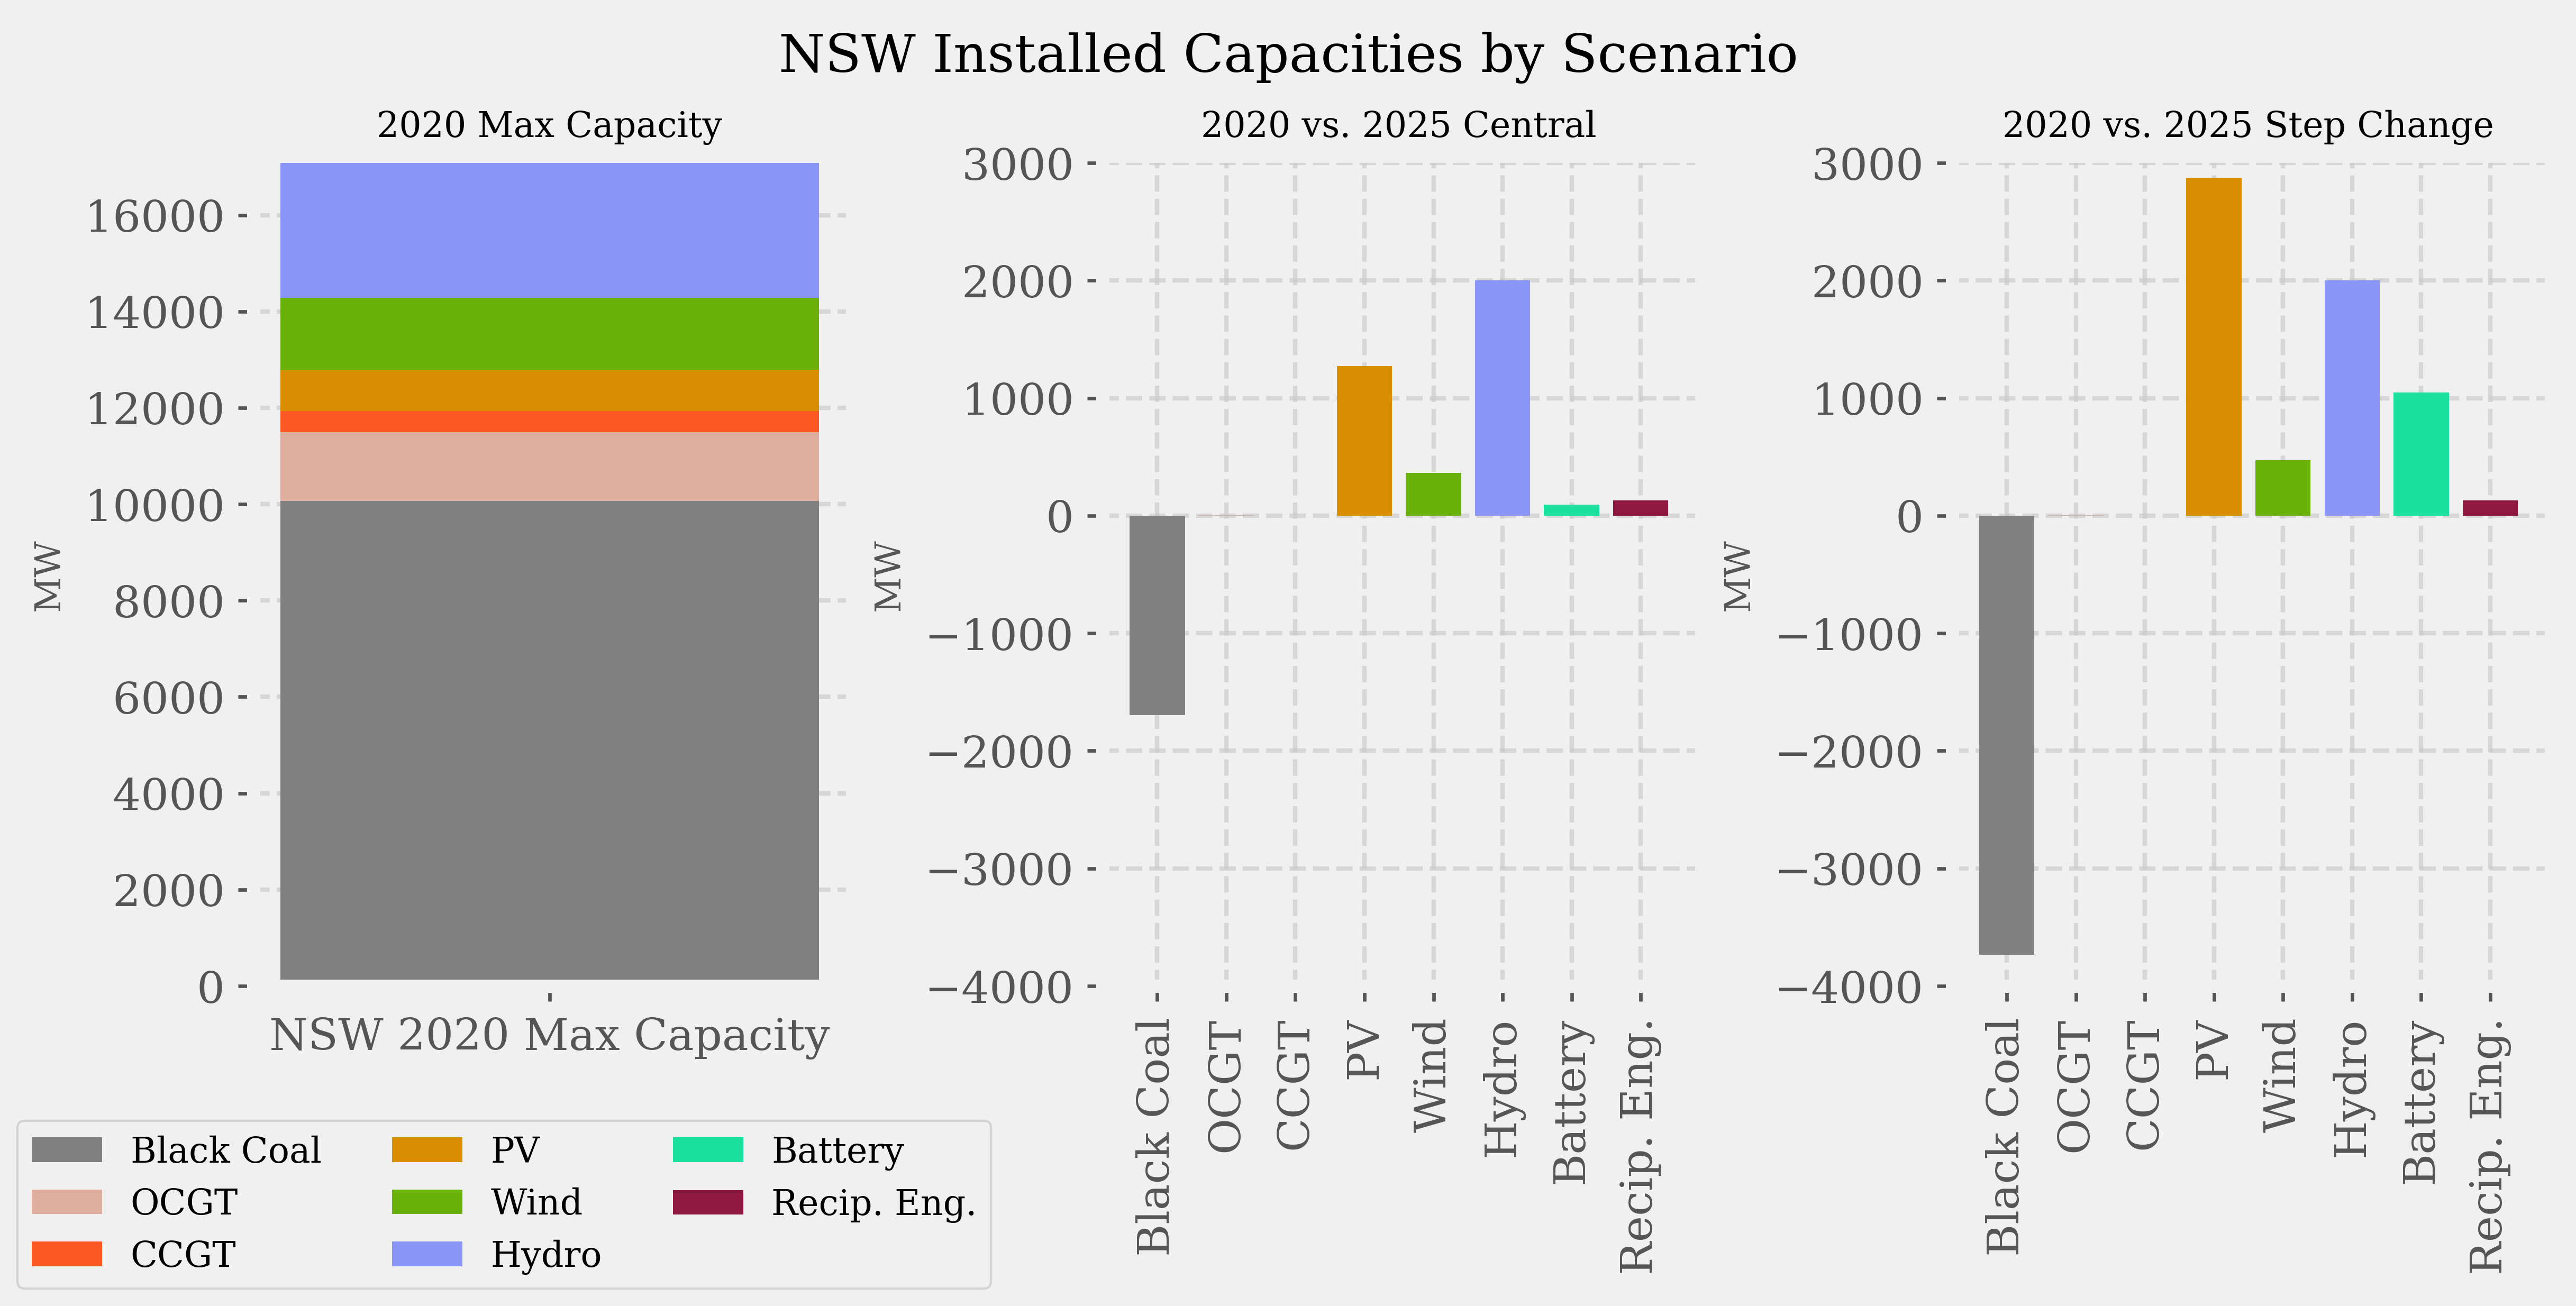
\includegraphics{source/figures/nsw_capacities.png}\label{fig:nsw_capacities}}

\subfloat[]{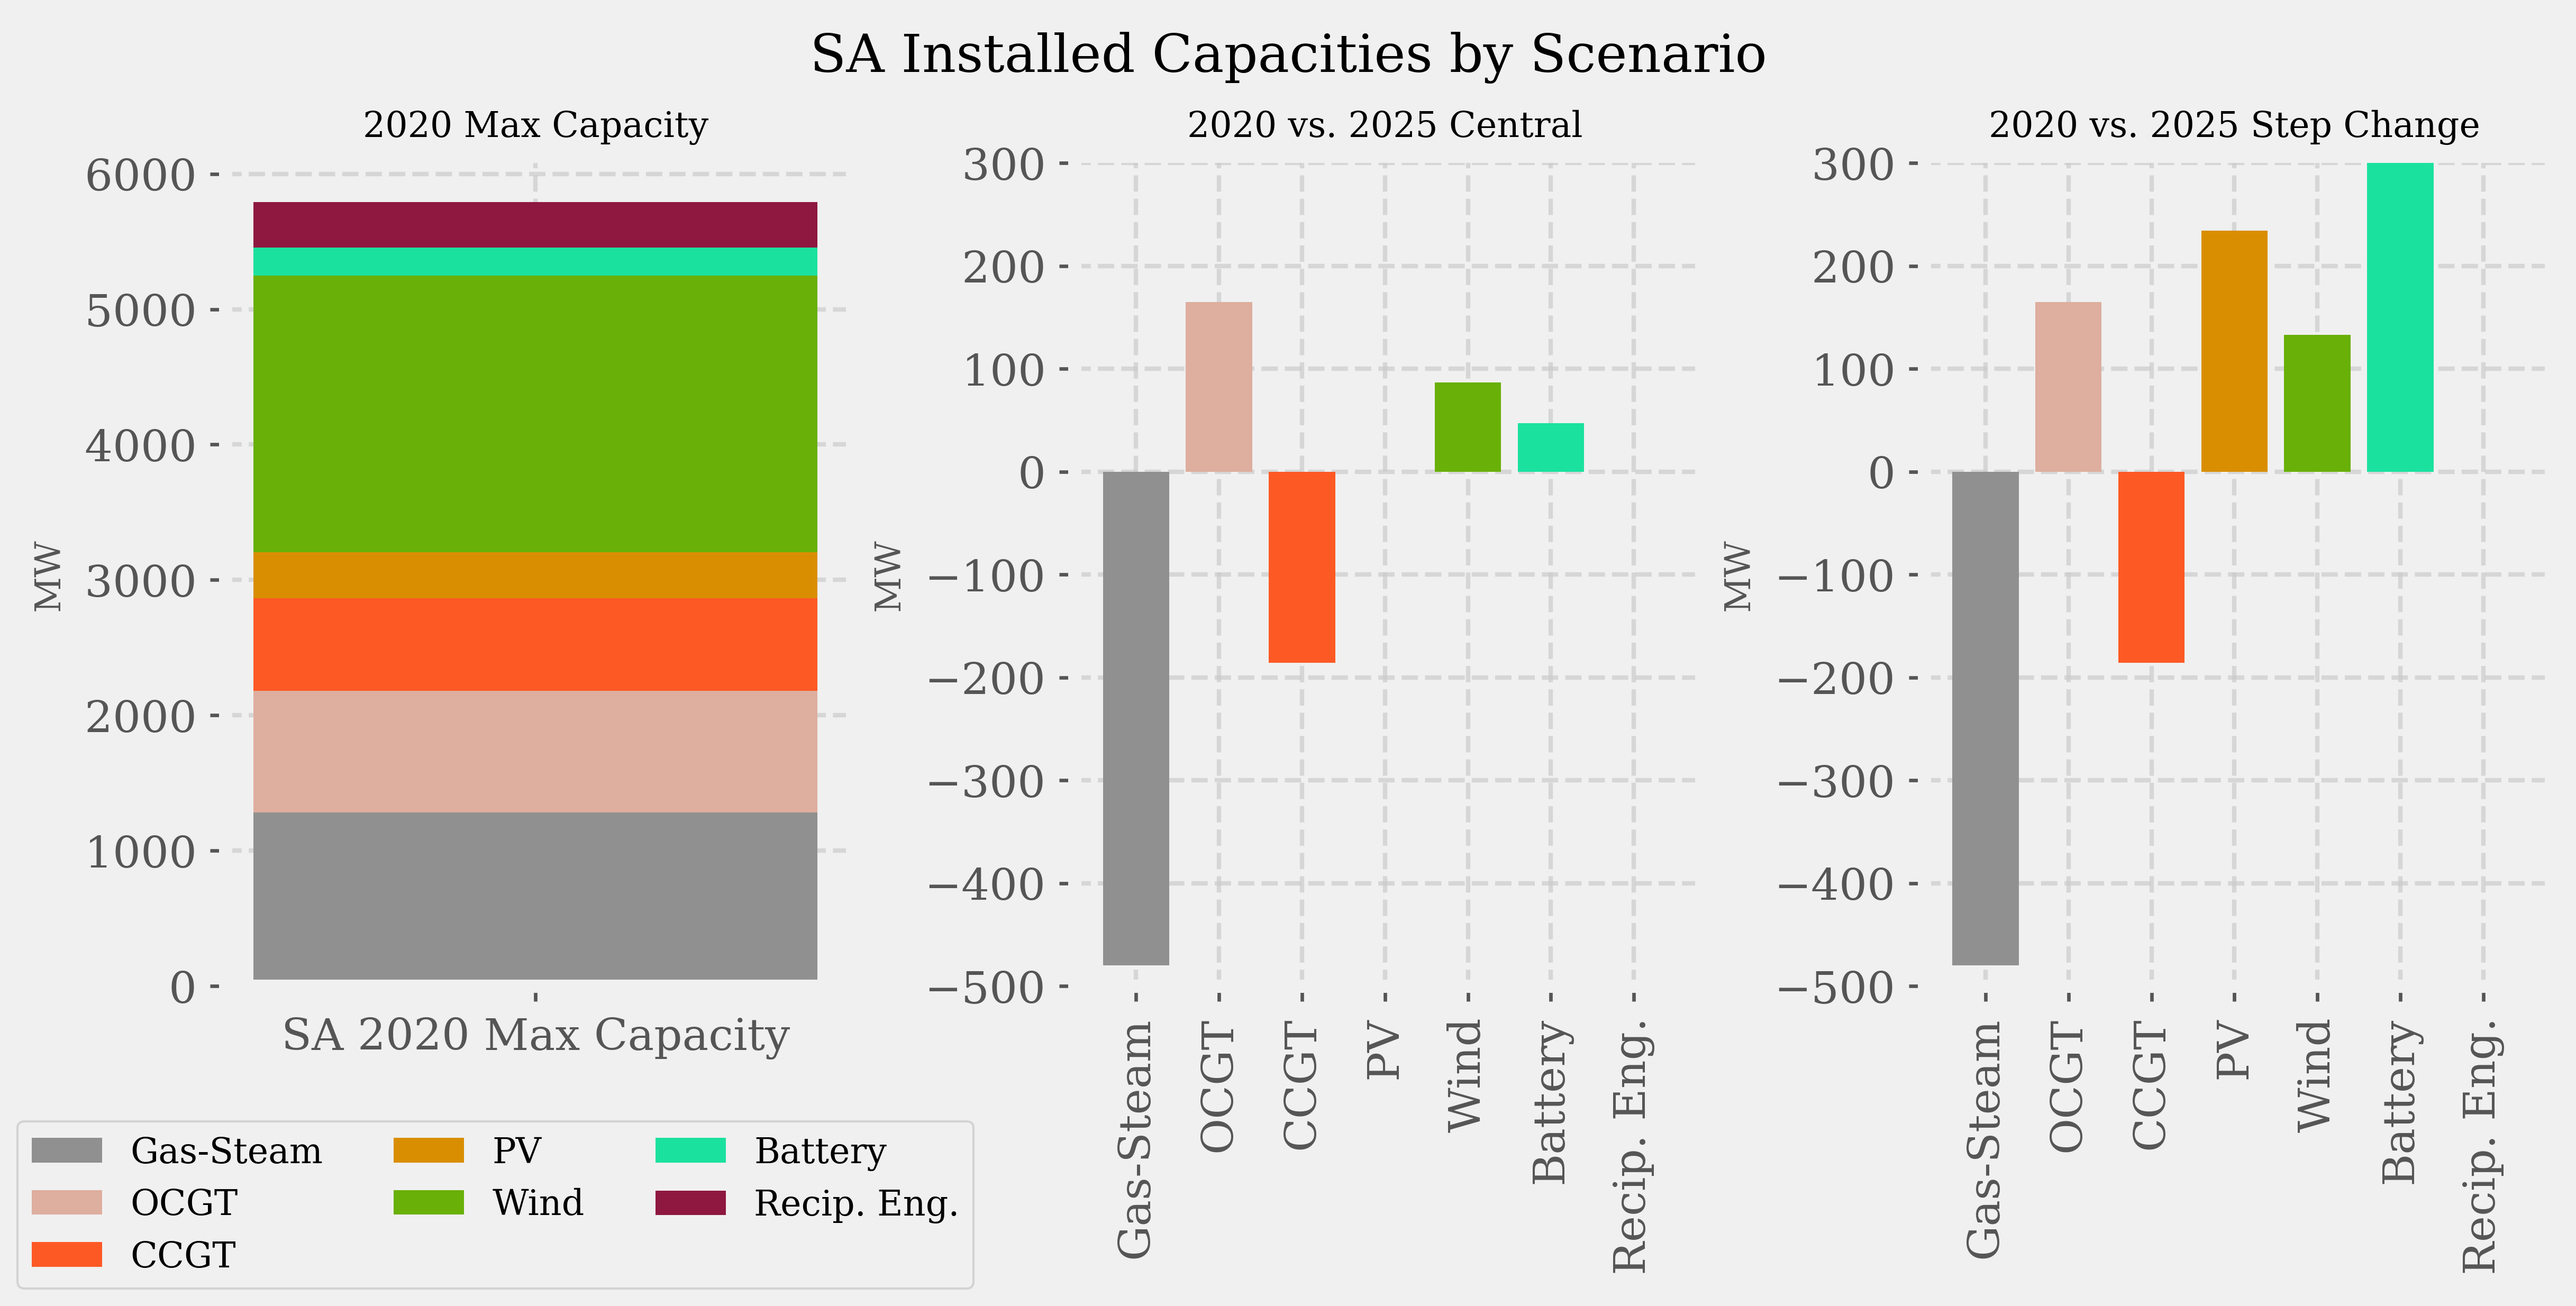
\includegraphics{source/figures/sa_capacities.png}\label{fig:sa_capacities}}

\caption[Capacity mix in NSW and SA in 2020 and the two 2025 scenarios]{Capacity mix in NSW (a) and SA (b) in
2020, and additional deployments and retirements in 2025 Central and
2025 Step Change. 2020 resource mixes were adapted from AEMO's 2020
Inputs and Assumptions workbook
(\protect\hyperlink{ref-australianenergymarketoperator2020InputsAssumptions2020}{Australian
Energy Market Operator, 2020p}). 2025 scenario resource mixes were
aligned with their namesake ISP scenarios
(\protect\hyperlink{ref-australianenergymarketoperator2020ISPGeneration2020}{Australian
Energy Market Operator, 2020o}) and include committed generation
(projects that are highly likely to proceed as they have acquired land,
secured financing, set a firm construction commencement date and either
finalised contracts for components or been granted planning approval)
(\protect\hyperlink{ref-australianenergymarketoperatorGenerationInformation2022}{Australian
Energy Market Operator, 2022c}).}

\label{fig:capacities}

\end{pandoccrossrefsubfigures}

\hypertarget{sec:reserves-method}{%
\subsection{Methodology}\label{sec:reserves-method}}

For each region and scenario, the available reserves and footroom in the
system were calculated from the results of a year-long time-sequential
market simulation implemented in the commercial electricity market
modelling tool PLEXOS
(\protect\hyperlink{ref-energyexemplarPLEXOSEnergyMarket2021}{Energy
Exemplar, 2021}). The PLEXOS market simulation consisted of a PASA phase
to model maintenance and forced outages for conventional generation
across the year, a Medium Term Schedule phase in NSW to schedule hydro
generation according to monthly energy constraints, and a Short Term
Schedule phase that carries out unit commitment and economic dispatch
(UC-ED) at 5-minute resolution in daily steps\footnote{A 12 hour
  look-ahead was used in the SA model to avoid ``end-of-horizon
  effects''
  (\protect\hyperlink{ref-barrowsIEEEReliabilityTest2020}{Barrows et
  al., 2020}), such as end-of-day decommitment of gas-fired generation.}.

Each existing coal-fired (NSW) and Gas-Steam (SA) unit was explicitly
modelled to accurately capture the consequences of partial and full
outages of large capacity units. For other resource types, the
operational constraints and attributes of individual units were averaged
and applied across all units of a resource type. This enabled clustered
UC-ED and thus reduced the computational burden of the Short Term
Schedule phase
(\protect\hyperlink{ref-palmintierHeterogeneousUnitClustering2014}{Palmintier
and Webster, 2014}). For baseload conventional generation and gas
turbines, ramp rates in each direction were separated into a
\emph{market} ramp rate, which was used in the PLEXOS market simulation,
and an \emph{upper} ramp rate, which was used to calculate available
reserves/footroom (Section~\ref{sec:reserves-conventionalcalc}). A lower
magnitude ramp rate in the market simulation (\emph{market}) reflects
participants' preferences to reduce cycling wear-and-tear due to
demanding ramping during typical operation (especially for ageing
assets) (\protect\hyperlink{ref-kumarPowerPlantCycling2012}{Kumar et
al., 2012}), whilst using a higher magnitude ramp rate to calculate a
resource's available reserves and footroom (\emph{upper}) ensures that
the total available flexibility of a resource can be utilised if needed
in a system emergency.

Both NSW and SA were modelled assuming a copper-plate network with no
interconnection to other regions (i.e.~single bus with no network
constraints). The Short Term Schedule mixed-integer linear program was
solved using the CPLEX Optimizer
(\protect\hyperlink{ref-ibmCPLEXOptimizer2021}{IBM, 2021}) with a
relative mixed-integer program gap tolerance of 0.07\%. The generation
and synchronisation status of each resource was obtained from the
solution and used to calculate the available reserves and footroom for
each 5-minute interval using the equations outlined in
Section~\ref{sec:reserves-modeloverview}. A process flow diagram of the
study methodology is shown in Figure~\ref{fig:method_diagram}.

In Appendix A, we outline our sources for key input data and assumptions
(top row of Figure~\ref{fig:method_diagram}) and provide further details
regarding how these data were used in the market simulation and/or the
calculation of available reserves and footroom.

\begin{figure}
\hypertarget{fig:method_diagram}{%
\centering
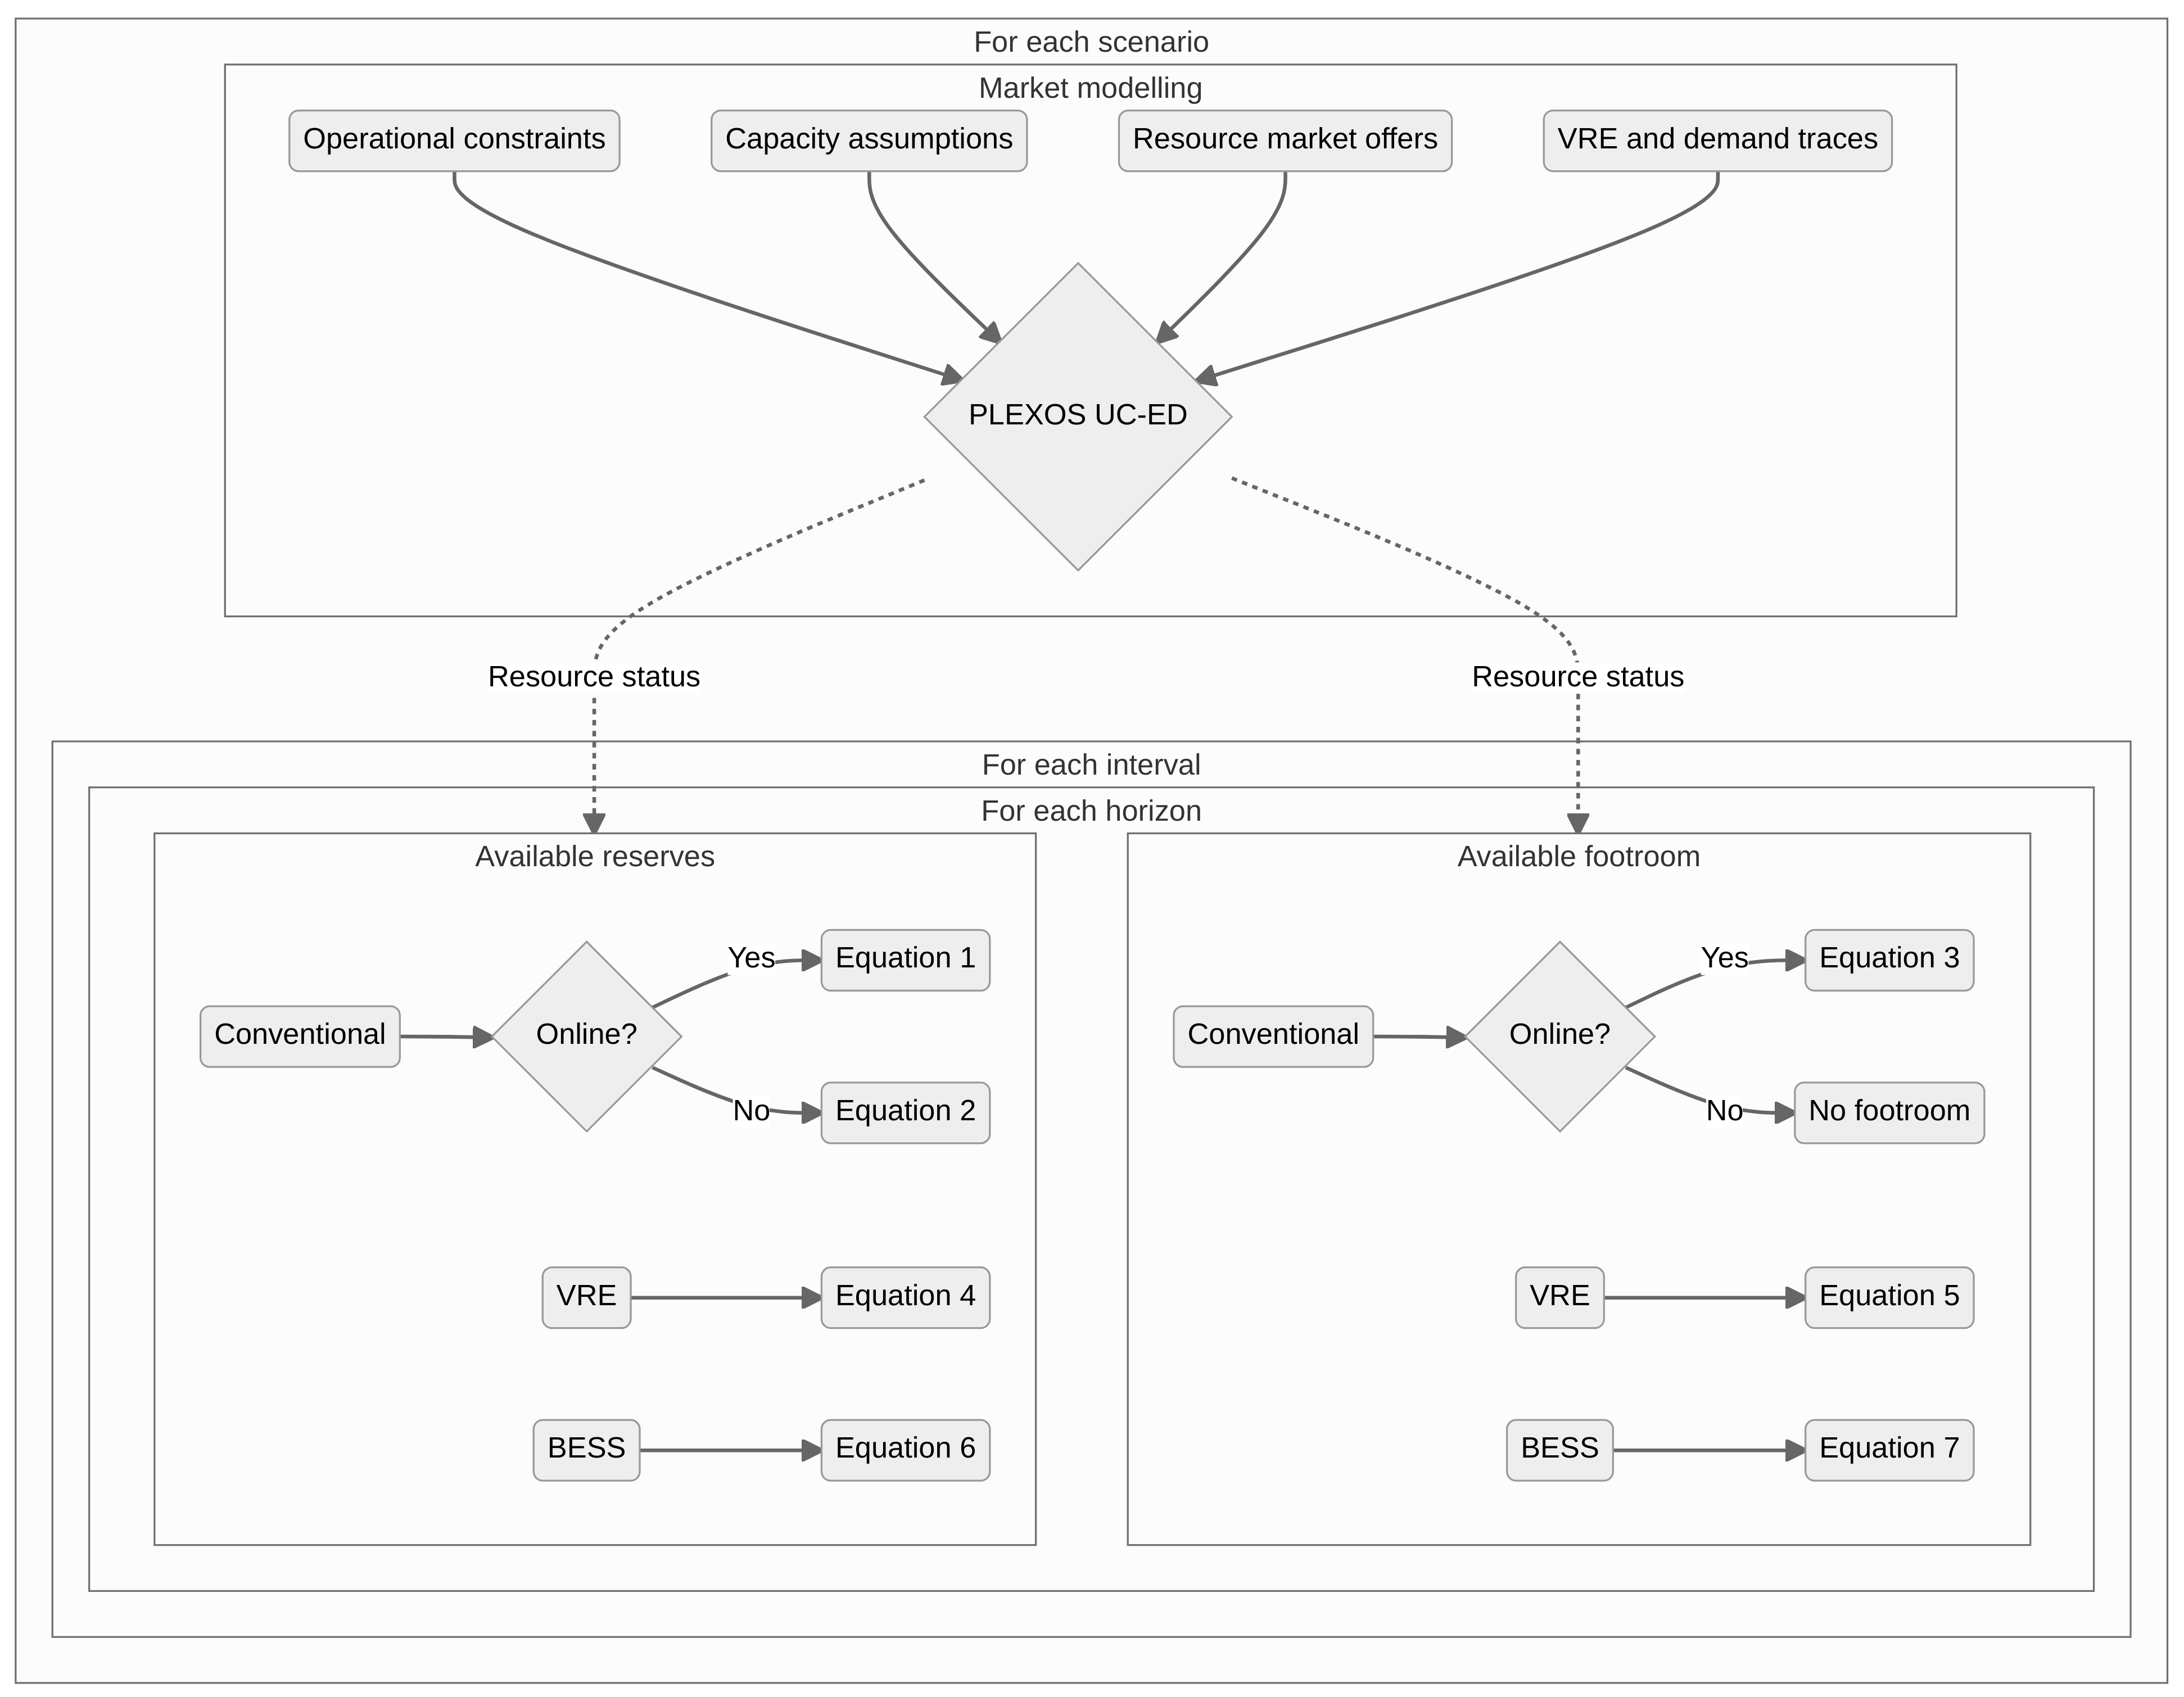
\includegraphics[width=1\textwidth,height=\textheight]{source/figures/modelling_diagram.png}
\caption[Process flow diagram for modelling available reserves and
footroom for each scenario]{Process flow for modelling available
reserves and footroom for each scenario in this case
study.}\label{fig:method_diagram}
}
\end{figure}

\hypertarget{limitations-1}{%
\subsection{Limitations}\label{limitations-1}}

There are two important caveats to this study. The first is that this
study models each region in isolation -- that is, resources in other NEM
regions can neither assist in meeting demand nor provide available
reserves or footroom through cross-regional interconnectors. During
typical operating conditions, it is likely that any headroom/footroom on
interconnectors would mean that a greater quantity of reserves/footroom
are available to a region, albeit at different horizons due to modified
dispatch patterns. For example, the inclusion of interconnectors in the
SA model between SA and VIC and SA and NSW\footnote{At the time of
  writing, the interconnector between SA and NSW is under construction
  and due to commence operation in 2025/2026
  (\protect\hyperlink{ref-electranettransgridProjectEnergyConnect}{ElectraNet,
  Transgrid, n.d.}).} may increase the total available reserves/footroom
in SA at the cost of a decrease in the reserves/footroom available
within shorter horizons. This could arise from local mid-merit gas
generators remaining offline in favour of inflexible but cheaper
coal-fired generation in NSW and VIC.

However, modelling available reserves and footroom for isolated regions
may provide a closer approximation to reality when balancing flexibility
is scarce in a region. Under these circumstances, it is likely that
interconnector flows will already be close to their limits. This will
reduce or altogether prevent the available reserves/footroom provision
from resources in neighbouring regions. Moreover, large interconnector
flows may be prevented if there is a credible risk of regional
separation (loss of synchronism between market regions due to
interconnector circuit faults --- a particular risk in the NEM due to
limited interconnection between market regions); at present, AEMO
co-optimises interconnector flow with regional FCAS procurement
(\protect\hyperlink{ref-australianenergymarketoperatorConstraintFormulationGuidelines2010}{Australian
Energy Market Operator, 2010}). An additional consideration is that if
an operating reserve product is implemented to improve the NEM's
resilience to supply-demand shocks, regional procurement requirements
may also limit the available reserves/footroom that can be procured over
an interconnector. As such, the modelling of isolated regions may
approximate actual operation when reserves/footroom are scarce and thus
most valuable to the system.

The second caveat is that this study does not explicitly model FCAS
procurement. If headroom or footroom reserved for FCAS is unable to also
provide available reserves or footroom\footnote{Exclusive headroom
  procurement for an operating reserve service (i.e.~inability to offer
  the same headroom in FCAS markets) is currently being considered
  (\protect\hyperlink{ref-energysecurityboardPost2025Market2021}{Energy
  Security Board, 2021a}).}, then modelling FCAS markets would reduce
the reserves and footroom that are available within horizons less than
or equal to 5 minutes. However, the actual headroom/footroom reduction
would depend upon the following factors:

\begin{itemize}
\tightlist
\item
  Whether regional FCAS procurement constraints bind for the modelled
  region. If they do not, multi-regional or NEM-wide FCAS requirements
  can be satisfied by procuring FCAS in other market regions.
\item
  The degree to which headroom/footroom is ``re-offered'' across
  sequential FCAS markets. For example, a single resource enabled for 10
  MW across the three raise contingency FCAS markets would withdraw less
  system headroom than three resources enabled for 10 MW each for a
  particular FCAS market.
\item
  Headroom that is offered into the 6 second and 60 second raise
  contingency FCAS market may not reflect sustained power provision. For
  example, frequency response from a steam-powered turbine may draw on
  steam stored in a boiler; a sustained response would require a longer
  timeframe due to slower boiler dynamics.
\end{itemize}

\hypertarget{sec:reserves-results}{%
\subsection{Results and discussion}\label{sec:reserves-results}}

\hypertarget{synthetic-daily-profiles}{%
\subsubsection{Synthetic daily
profiles}\label{synthetic-daily-profiles}}

\emph{Synthetic daily profiles} (SDPs) were developed to quantify the
time-varying spectrum of available reserves and footroom for each
scenario. For a given horizon, the SDP value at a particular time is an
aggregate value (mean or a specific percentile) calculated from the
reserves/footroom available within that horizon at the end of that
dispatch interval across all days in the simulated year. In other words,
values from across the year for a given time of day are aggregated, and
these are then ``stitched'' together to form a ``synthetic day'' curve
for a particular horizon. Two aggregate values were calculated for each
horizon curve:

\begin{enumerate}
\def\labelenumi{\arabic{enumi}.}
\tightlist
\item
  The mean. This provides a picture of the average or ``typical''
  availability of reserves and footroom at different times of the day
  for a particular scenario year; and
\item
  The bottom 1\% (i.e.~1\textsuperscript{st} percentile or 1-in-100 day
  lowest). This measure better reflects the availability of reserves and
  footroom when they are scarce and thus when they are most
  needed\footnote{More extreme percentiles (i.e.~\textless{} 1\%) could
    better reflect the tight reliability standards adopted in many power
    systems - e.g.~the NEM standard of a maximum expected unserved
    energy of 0.002\% of the total energy demand of a NEM region in an
    Australian financial year
    (\protect\hyperlink{ref-australianenergymarketcommissionreliabilitypanel2022ReviewReliability2022}{Australian
    Energy Market Commission Reliability Panel, 2022}). However, the use
    of extreme percentiles would be more appropriate with a greater
    number of modelled days (i.e.~several years).}.
\end{enumerate}

In addition to an infinite horizon (which corresponds to the maximum
availability), curves were calculated for 1, 5, 15, 30 and 60 minute
horizons. These horizons encompass the start-up times of hydro and
flexible gas generation, and represent the likely timeframes over which
the proposed operating reserve product will be required to respond.

\hypertarget{sec:reserves-reserveSDPs}{%
\subsubsection{Available reserve synthetic
days}\label{sec:reserves-reserveSDPs}}

Mean and bottom 1\% available reserve SDPs were generated for the NSW
scenarios and for the SA scenarios
(Figures~\ref{fig:nswreserves}, \ref{fig:sareserves}). The mean SDPs
across scenarios suggest that, on average, NSW has more than 2 GW and SA
more than 600 MW of reserves available within 5+ minutes. These levels
of reserves:

\begin{enumerate}
\def\labelenumi{\arabic{enumi}.}
\tightlist
\item
  Correspond to approximately 15\% and 20\% of peak demand in 2020 in
  NSW and SA, respectively. These 5+ minute ``reserve margins'' (i.e.~5+
  minute reserves as a percentage of peak demand) are comparable to
  lower-end reserve margins anticipated for the summer of 2022 in North
  American jurisdictions
  (\protect\hyperlink{ref-northamericanelectricreliabilitycorporation2022SummerReliability2022}{North
  American Electric Reliability Corporation, 2022}).
\item
  Exceed the highest N-1 contingency in 2020 (i.e.~highest LOR2 trigger
  level declared in the last run of Pre-Dispatch PASA prior to delivery
  --- see Section~\ref{sec:reserves-ahead_soint}) by approximately 225\%
  in NSW and 170\% in SA
  (\protect\hyperlink{ref-prakashNEMSEERPythonPackage2023}{Prakash et
  al., 2023b}).
\end{enumerate}

Furthermore, with additional BESS and flexible gas resources expected to
be deployed, the mean 5+ minute reserve margins of both regions are
higher for most parts of the day in the 2025 Step Change scenario.
Though the market simulation relied on perfect foresight (additional
uncertainty may reduce reserve margins), these results suggest that
reasonable quantities of reserves are available in each region within a
5+ minute horizon.

\begin{figure}
\hypertarget{fig:nswreserves}{%
\centering
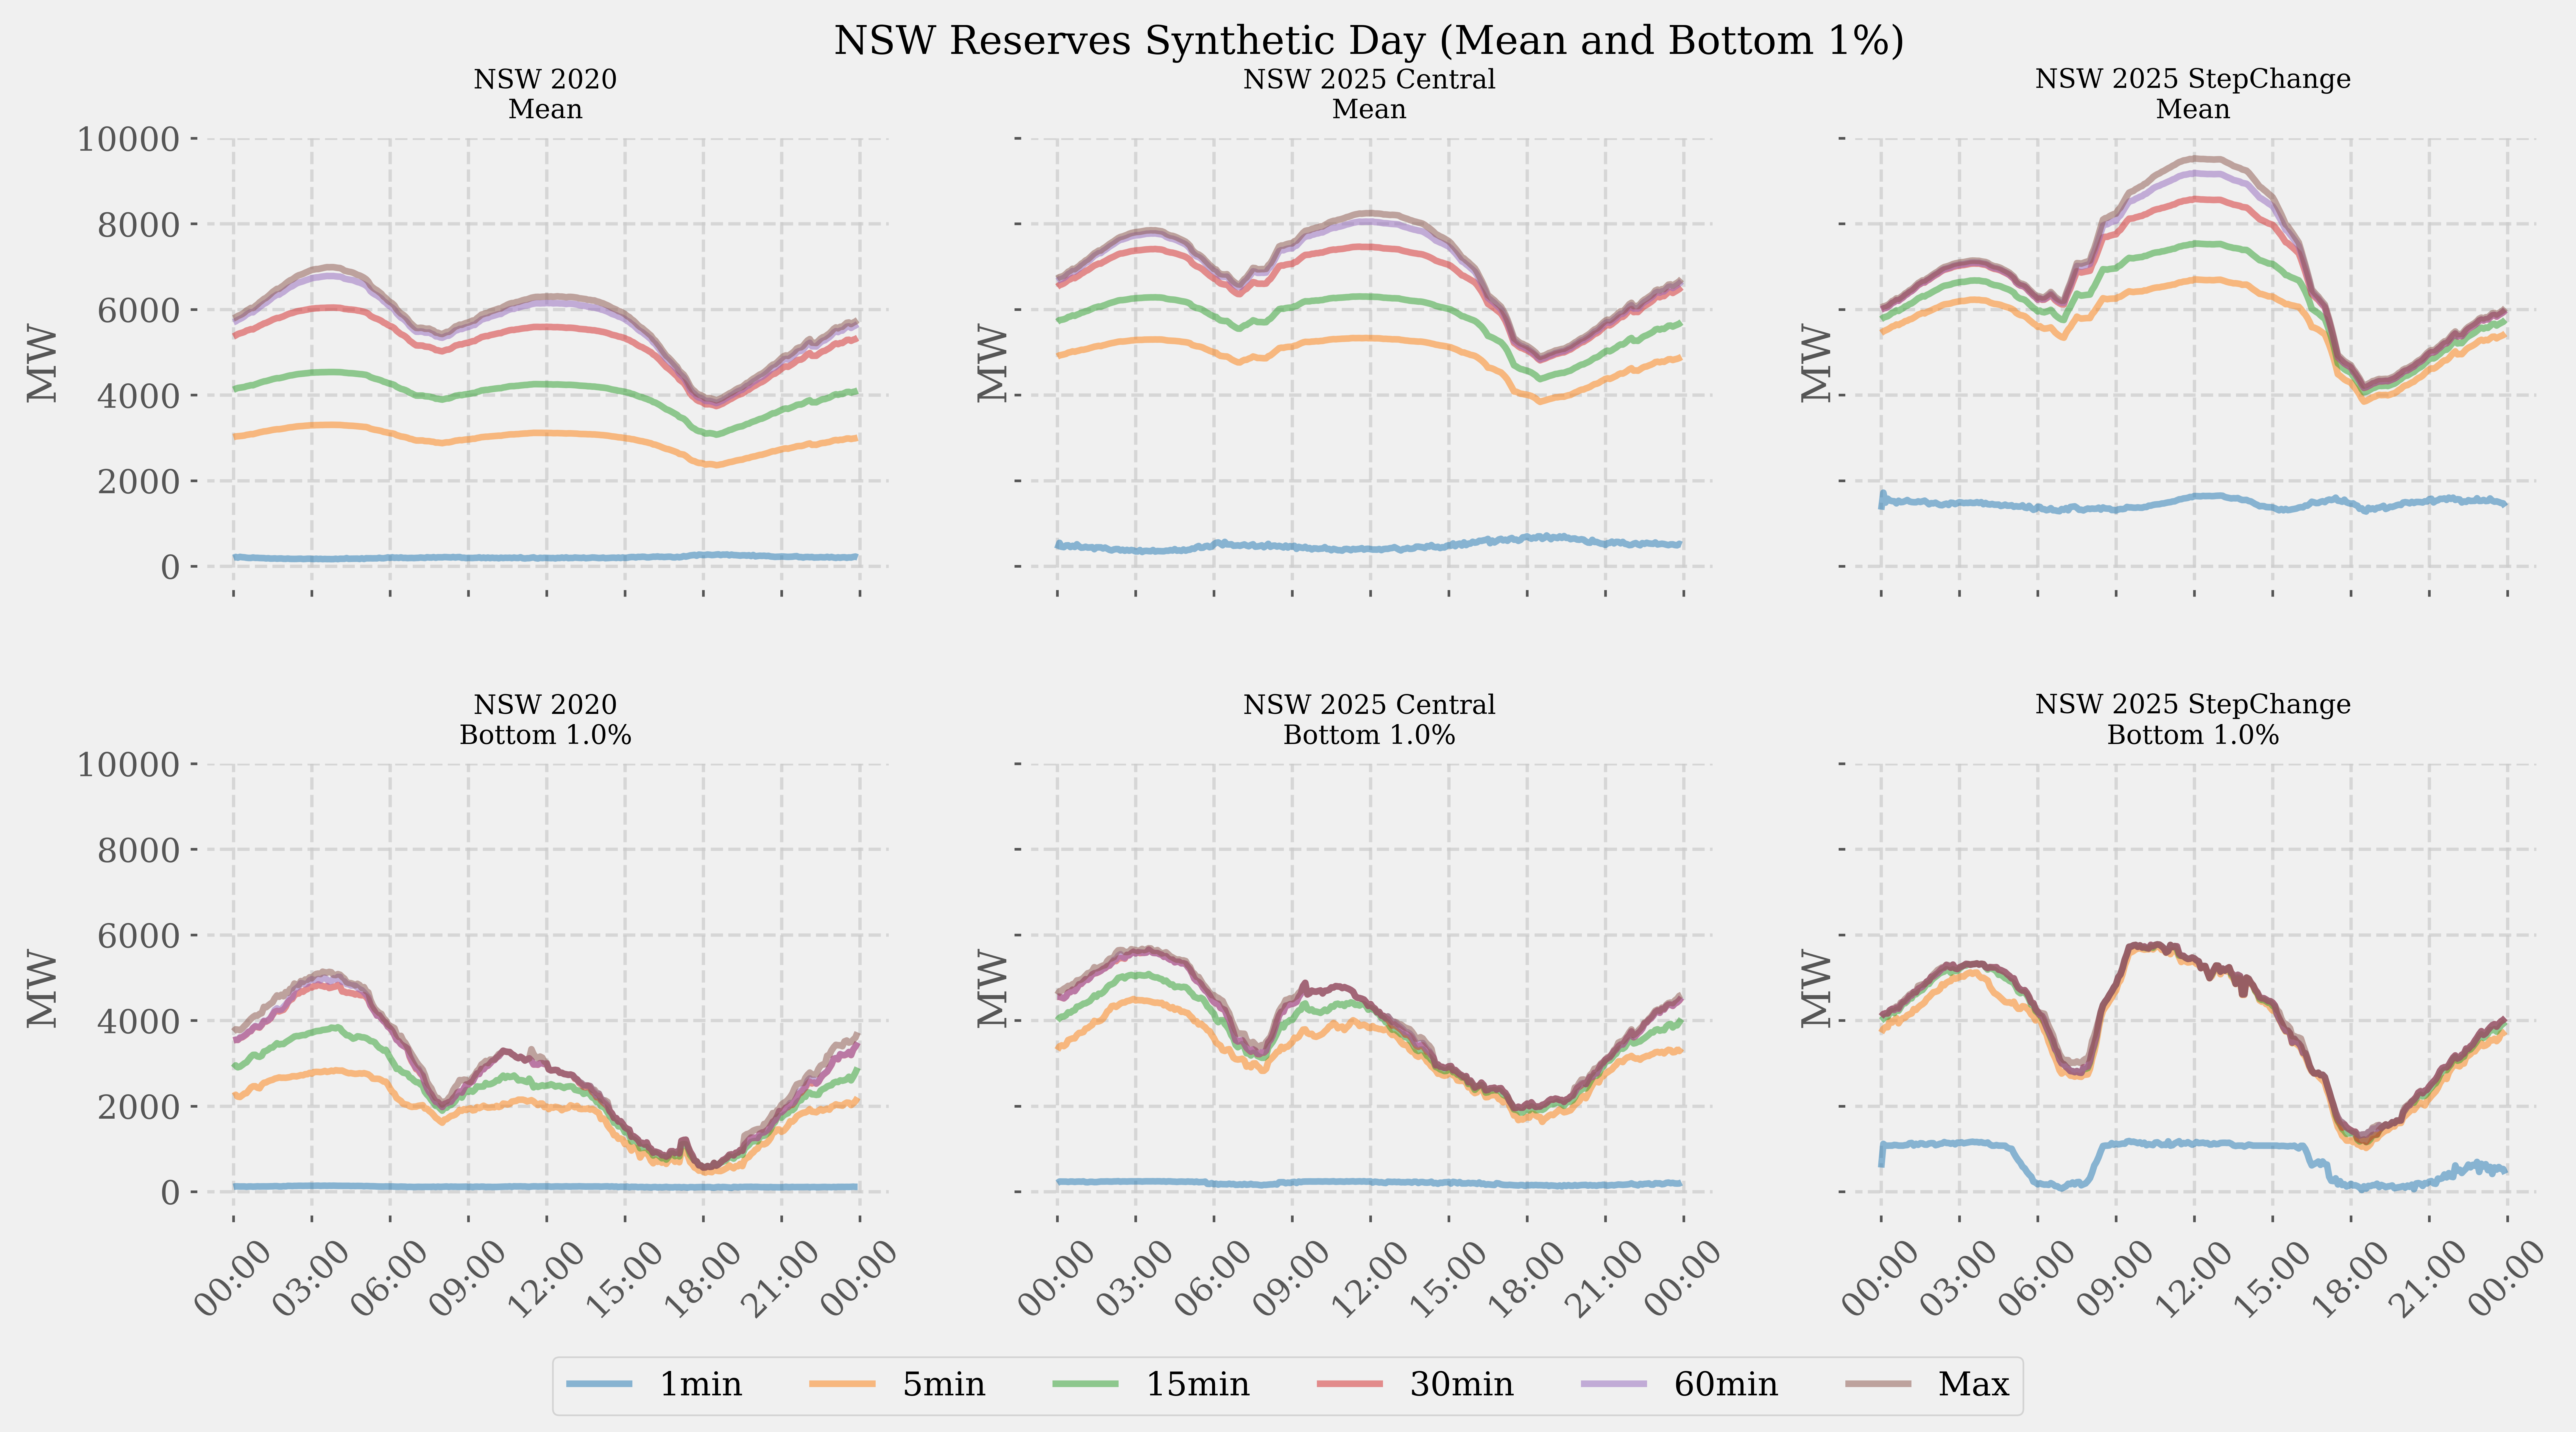
\includegraphics[width=1\textwidth,height=\textheight]{./source/figures/NSW_reserves_all_profiles_by_di.png}
\caption[NSW available reserves SDPs]{Mean (top row) and bottom 1\%
(bottom row) SDPs for available reserves in NSW in 2020 (leftmost
column) and the two 2025 scenarios (rightmost
columns).}\label{fig:nswreserves}
}
\end{figure}

\begin{figure}
\hypertarget{fig:sareserves}{%
\centering
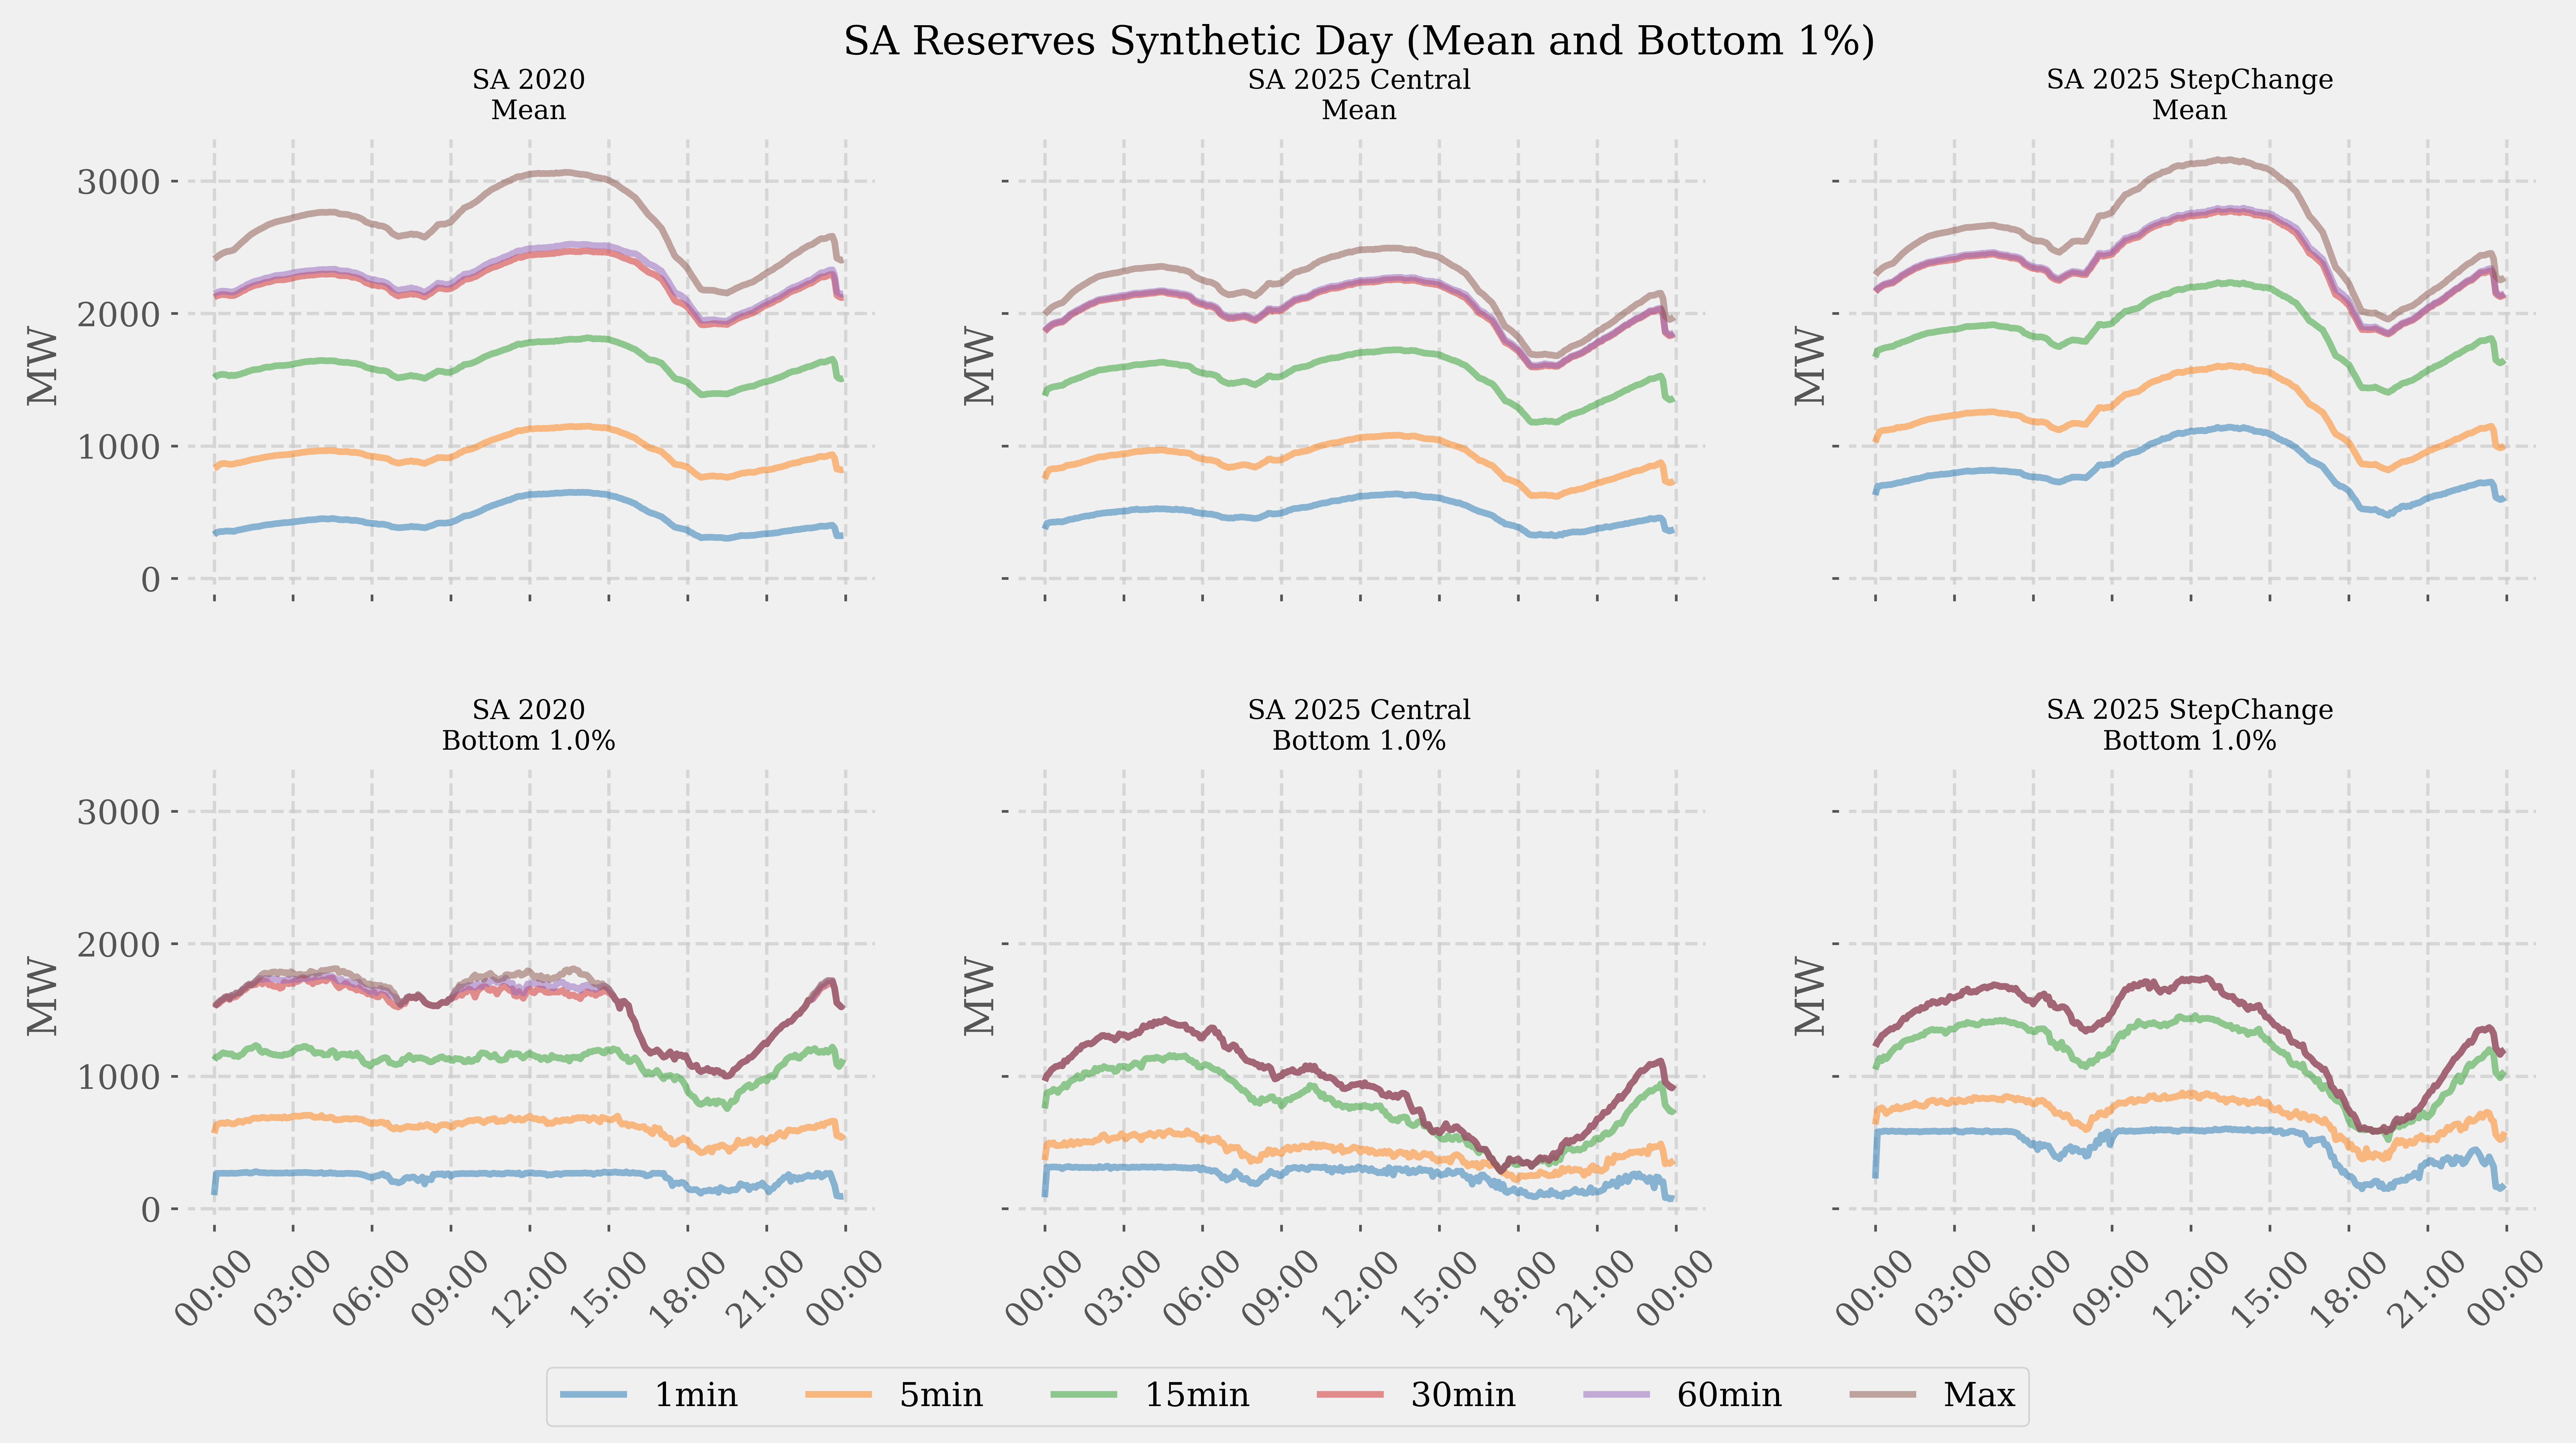
\includegraphics[width=1\textwidth,height=\textheight]{./source/figures/SA_reserves_all_profiles_by_di.png}
\caption[SA available reserves SDPs]{Mean (top row) and bottom 1\%
(bottom row) SDPs for available reserves in SA in 2020 (leftmost column)
and the two 2025 scenarios (rightmost columns).}\label{fig:sareserves}
}
\end{figure}

Across scenarios, the following trends are apparent in the SDPs:

\begin{enumerate}
\def\labelenumi{\arabic{enumi}.}
\tightlist
\item
  From 2020 to the 2025 Step Change scenario, a midday peak in the mean
  available reserves SDPs becomes more pronounced. This can be
  attributed to the increasing displacement of conventional generation
  by lower-cost utility-scale solar PV in dispatch (an outcome observed
  by Hummon et al.
  (\protect\hyperlink{ref-hummonFundamentalDriversCost2013}{2013}) and
  Tanoto et al.
  (\protect\hyperlink{ref-tanotoImpactHighSolar2021}{2021})) and the
  progressive erosion of daytime operational demand due to higher
  penetrations of distributed solar PV. Particularly in SA, curtailed
  VRE and BESS also contribute to this reserve ``surplus''. BESS in
  particular are often charging during such periods of plentiful supply
  and low prices, and thus are able to offer up to double their active
  power rating as reserve (i.e.~by switching from charging to
  discharging).
\item
  As is particularly clear in the bottom 1\% SDPs for the 2025
  scenarios, the availabilities of different reserve horizons tend to
  converge during periods of lower reserves or ``relative scarcity'',
  which include peak demand events in the morning and evening. The
  convergence may be driven by the retirement of baseload conventional
  generation and higher ramping requirements in the 2025 scenarios
  requiring more flexible, mid-merit resources to be online prior to and
  during these periods.
\end{enumerate}

From this analysis, we can also gain an insight into the supply-side
dynamics of a potential operating reserve product market. The first
trend suggests that as energy transition proceeds, a reserve surplus
during the daytime could suppress the price of an operating reserve
product (a dynamic that is further explored by Frew et al.
(\protect\hyperlink{ref-frewCurtailmentParadoxTransition2021}{2021b})).
Moreover, the convergence of availability across horizons during periods
of ``relative scarcity'' suggests that relatively inflexible but cheaper
resources are being preferentially ramped through dispatch at these
times whilst more flexible but expensive resources are left in reserve.
Since the majority of system headroom during these periods appears to be
available within 5 to 15 minutes, operating reserves would likely be
procured from these more flexible resources regardless of whether the
product requires availability within 5 or 30 minutes. As such, concerns
regarding limited providers of a 5-minute horizon product may also apply
to a 30-minute horizon product during periods of relative scarcity
(noting that several resource types in the NEM are already providing
upwards flexibility within 5 minutes in the NEM, as shown in
Figure~\ref{fig:raise_delayed_supply}).

\hypertarget{sec:reserves-footroomSDPs}{%
\subsubsection{Available footroom synthetic
days}\label{sec:reserves-footroomSDPs}}

Two types of SDPs were constructed for available footroom: one for
\emph{firm} footroom and the other for total footroom. The former refers
to potential footroom provision from conventional resources and BESS,
whereas the latter also includes footroom that can be provided by
curtailing VRE. Figures~\ref{fig:nswfirmfoot}, \ref{fig:nswfoot} show
mean and bottom 1\% SDPs across NSW scenarios for firm footroom and
total footroom, respectively. From the bottom 1\% SDPs in
Figure~\ref{fig:nswfirmfoot}, it is clear that firm system footroom can
become very low in NSW in 2025 as remaining baseload conventional
generators are driven to operate closer to their MSLs. However, such
concerns could be alleviated if VRE provide footroom
(Figure~\ref{fig:nswfoot}). A similar result was observed for the SA
region.

\begin{figure}
\hypertarget{fig:nswfirmfoot}{%
\centering
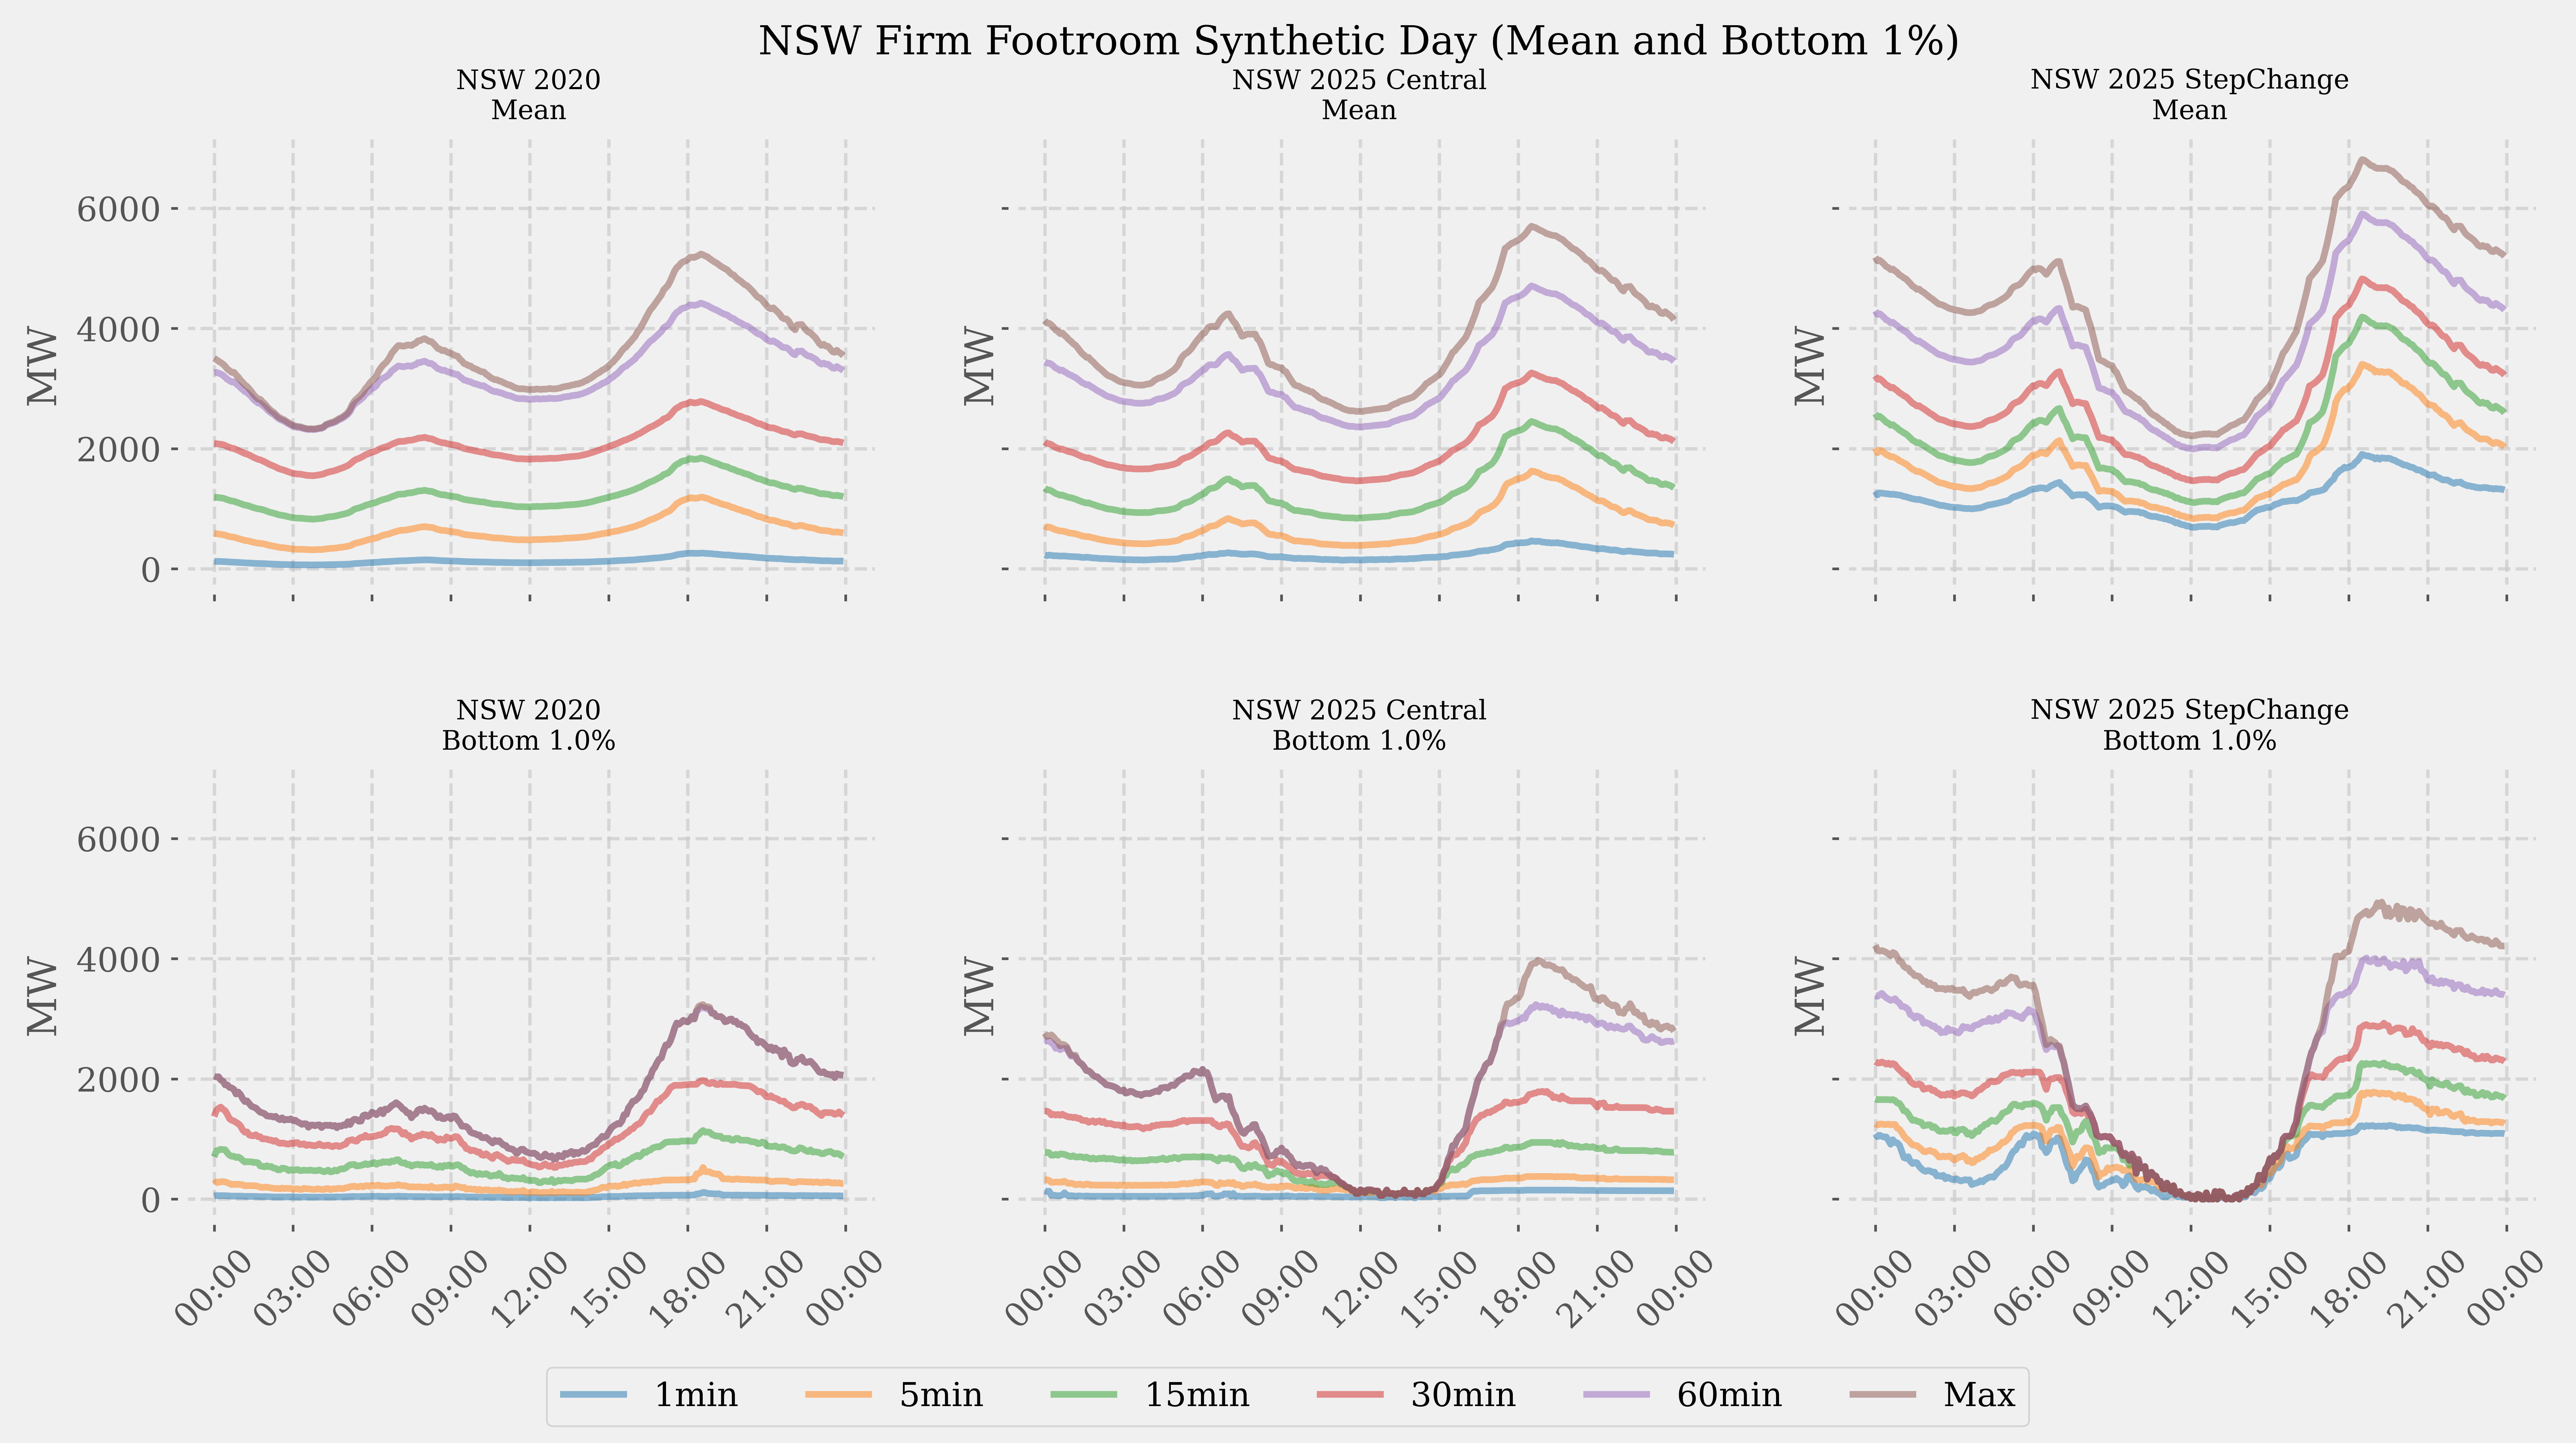
\includegraphics[width=1\textwidth,height=\textheight]{./source/figures/NSW_firmfootroom_all_profiles_by_di.png}
\caption[NSW firm footroom SDPs]{Mean (top row) and bottom 1\% (bottom
row) SDPs for available firm footroom (i.e.~footroom provided only by
``firm'' resources: conventional and BESS) in NSW in 2020 (leftmost
column) and the two 2025 scenarios (rightmost
columns).}\label{fig:nswfirmfoot}
}
\end{figure}

\begin{figure}
\hypertarget{fig:nswfoot}{%
\centering
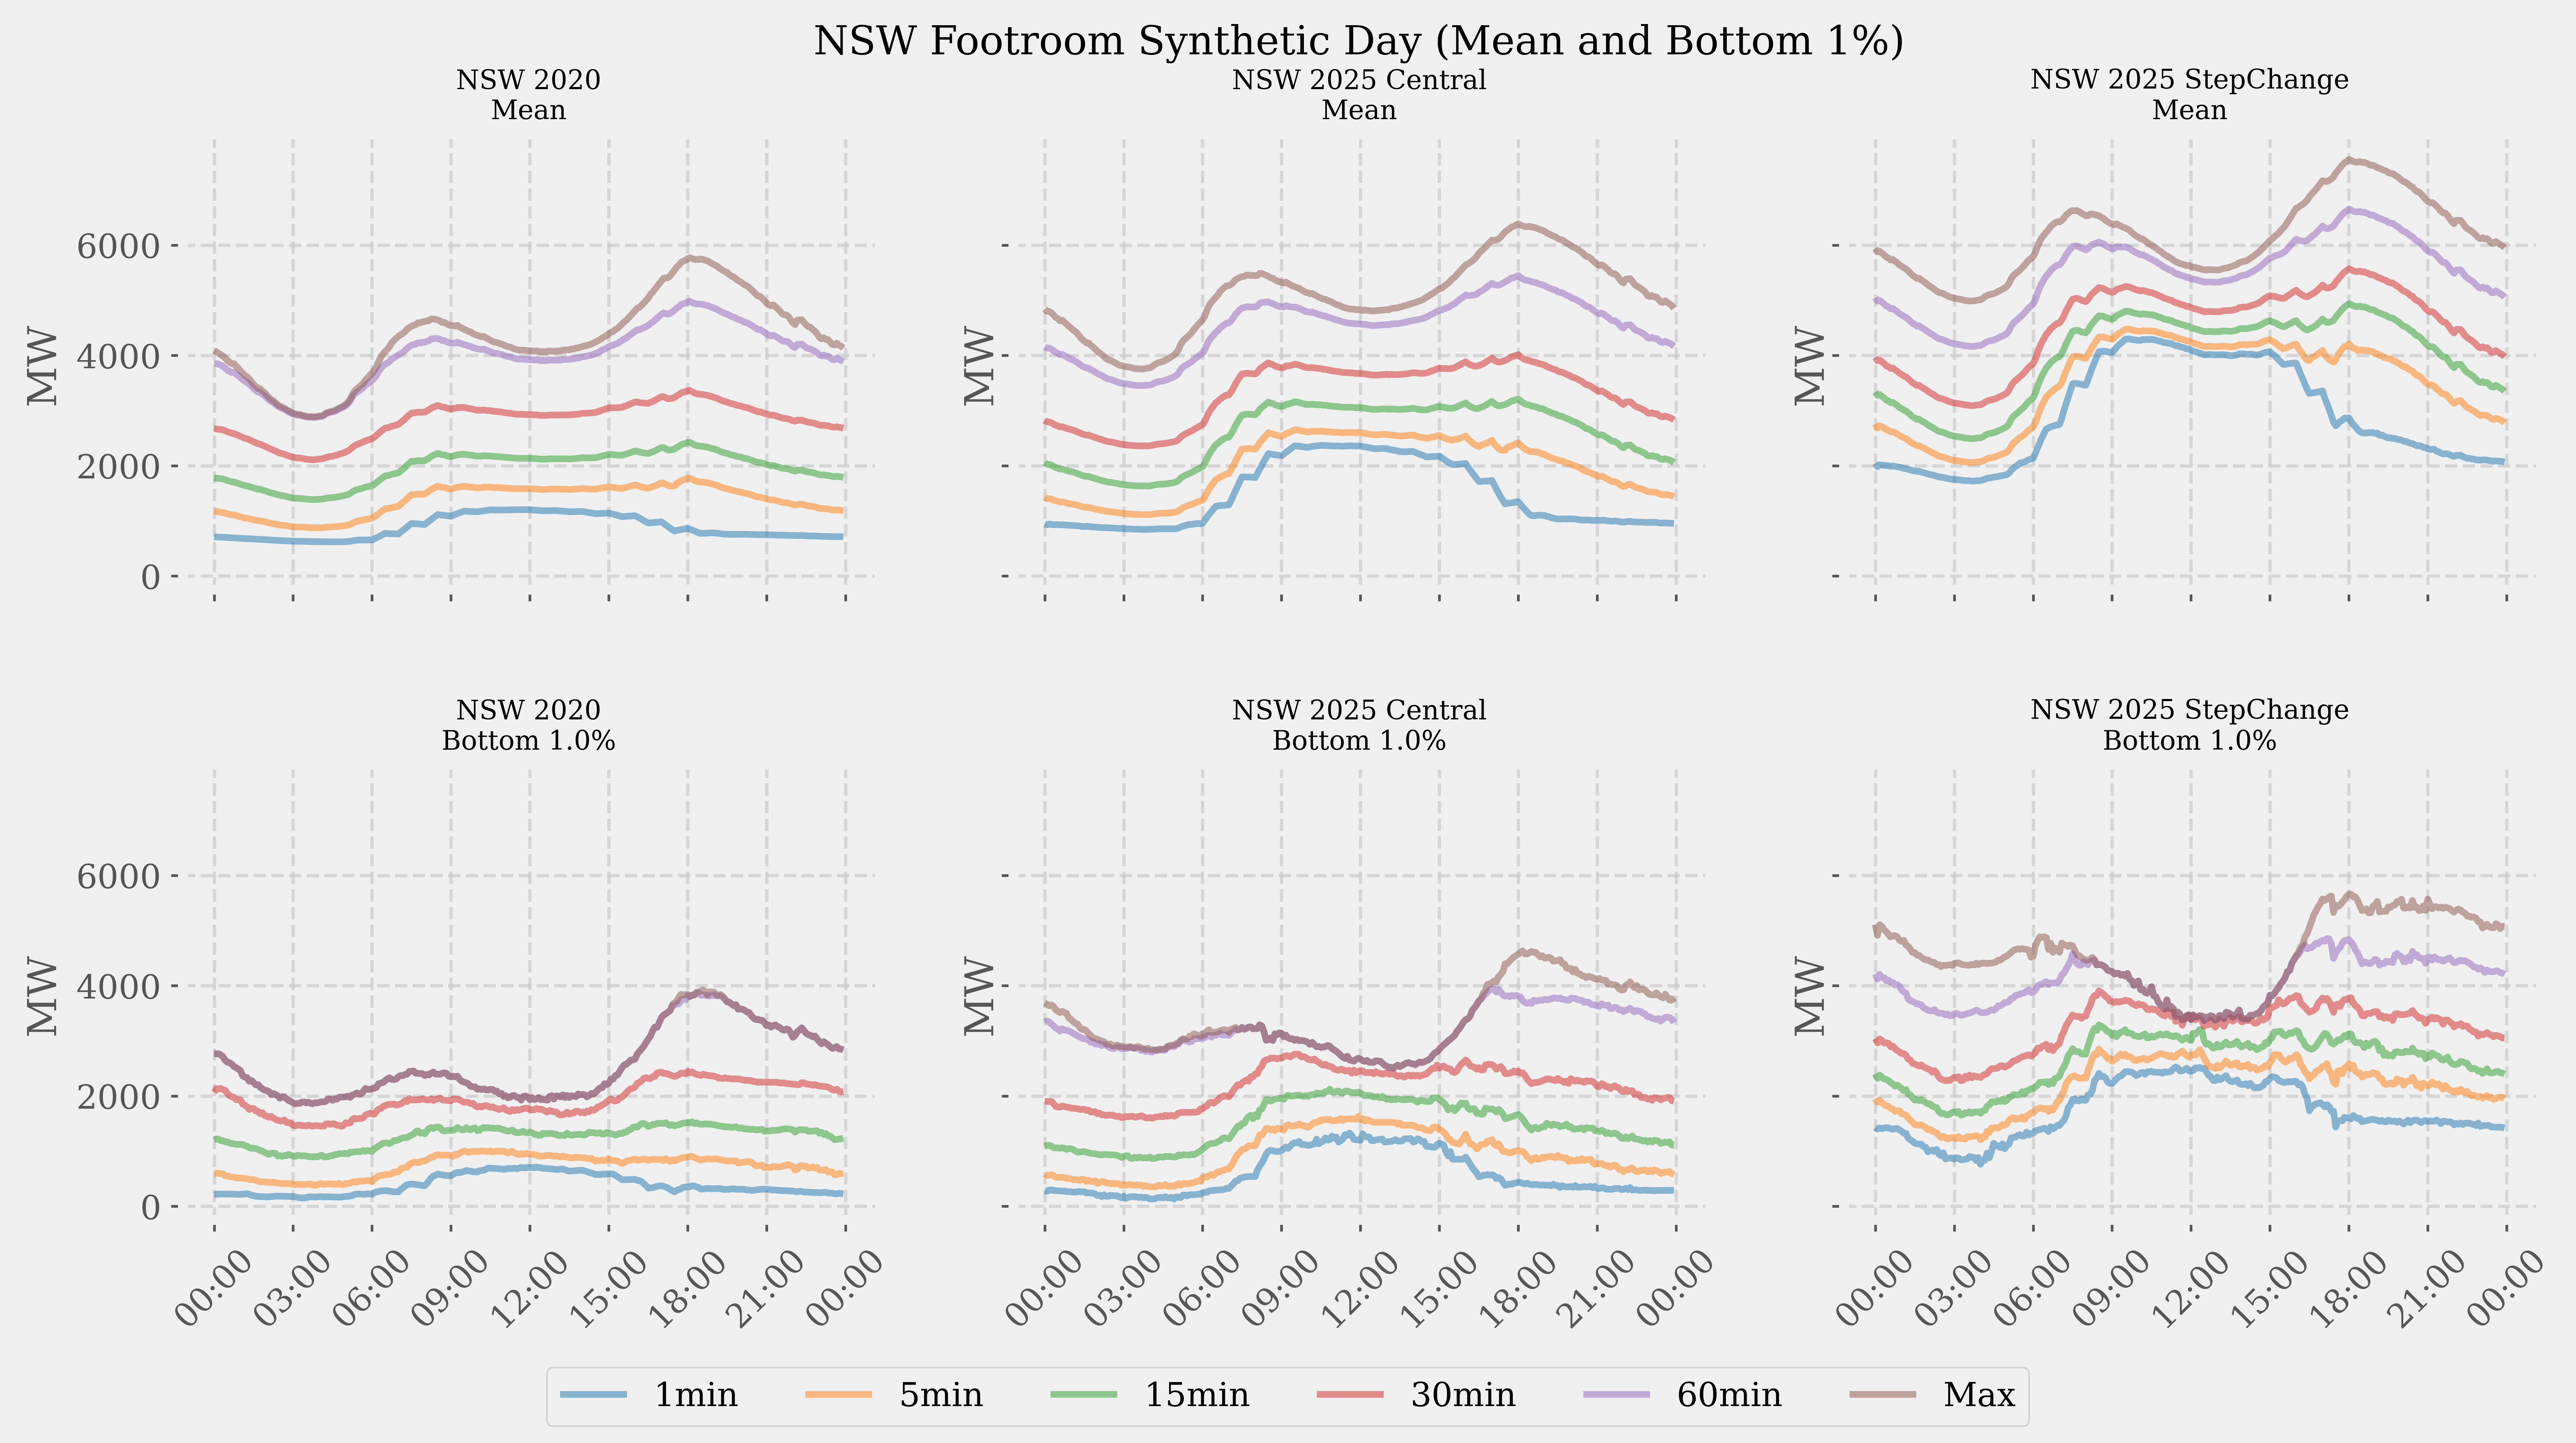
\includegraphics[width=1\textwidth,height=\textheight]{./source/figures/NSW_footroom_all_profiles_by_di.png}
\caption[NSW footroom SDPs]{Mean (top row) and bottom 1\% (bottom row)
SDPs for available total footroom (including footroom that would be
provided by curtailing VRE) in NSW in 2020 (leftmost column) and the two
2025 scenarios (rightmost columns).}\label{fig:nswfoot}
}
\end{figure}

The available footroom in the system is likely sensitive to extent of
conventional generation retirements. Further retirements may enable
remaining conventional resources to operate at a higher loading, thereby
increasing the available footroom in the system. Regardless, given that
each region appears to suffer a lack of \emph{firm} footroom for several
hours during the day in the 2025 scenarios explored in this case study,
mechanisms for procuring sustained downwards balancing flexibility
should be considered alongside those for procuring sustained upwards
balancing flexibility. One simple option would be to implement an
operating \emph{footroom} product, which, if VRE are permitted to
provide this service, can enable conventional generation to operate
closer to their MSL and thus reduce system operating costs and carbon
emissions
(\protect\hyperlink{ref-nelsonInvestigatingEconomicValue2018}{Nelson et
al., 2018}).

\hypertarget{sec:reserves-stelr}{%
\subsubsection{Short-term energy-limited
reserves}\label{sec:reserves-stelr}}

While the available reserves metric does not consider the duration for
which reserve deployment can be sustained, we can infer whether reserves
are short-term energy-limited (i.e.~with a duration no more than a few
hours) based on their resource type. For this analysis, BESS reserve
power was calculated based on the BESS's state of charge at the end of
each dispatch interval and the requirement to sustain provision for 15
minutes. This duration is consistent with the BESS power and capacity
that is reserved in SA for the possibility of loss of interconnection
(\protect\hyperlink{ref-australianenergymarketoperator2020SystemStrength2020}{Australian
Energy Market Operator, 2020q}). In addition, the maximum available
price-responsive demand available in each state was added to the
available reserves in each dispatch interval (assuming an emergency
response time of 5 minutes) to gain a better understanding of the
maximum potential contribution of demand response. This corresponded to
\textasciitilde60 MW in SA and \textasciitilde290 MW in NSW, based on
AEMO analysis and forecasts in Australian Energy Market Operator
(\protect\hyperlink{ref-australianenergymarketoperator2020InputsAssumptions2020}{2020p}).
Both BESS and DR can be considered to be short-term energy-limited
reserve providers. Though conventional generation fuel constraints (e.g
reservoir schemes and the gas system) were not modelled in this market
simulation, the contribution of conventional resources was separated
into those of thermal and hydro to assess the importance of the energy
constraints on each resource type to available reserves in NSW.

Tables \ref{tab:nsw_stel} and \ref{tab:sa_stel} show the median
percentage across dispatch intervals in a scenario year of available
reserves provided by a resources type for NSW and SA, respectively.
Whilst hydro and thermal resources dominate 5 minute horizon reserve
provision in 2020 in NSW and SA, respectively, short-term energy limited
resources provide a greater proportion of reserves in this horizon in
2025. In particular, the median contribution of BESS to reserves
available within 5 minutes is 16\% for NSW and 40\% for SA in the 2025
Step Change scenario. As the reserve horizon is extended to 30 minutes,
a greater proportion of reserves are provided by conventional resources,
which may be better positioned to sustain a response beyond the
short-term\footnote{In reality, conventional resources are also
  susceptible to fuel constraints, as highlighted by the events
  preceding the 2022 NEM suspension
  (\protect\hyperlink{ref-australianenergymarketoperatorNEMMarketSuspension2022}{Australian
  Energy Market Operator, 2022d}). More sophisticated modelling of
  thermal coal availability, the gas system and hydro schemes, including
  their operation under different climate conditions, would be required
  to better understand the potential duration of available reserve
  provided by conventional generation.}. These results indicate that as
energy transition progresses, a trade-off between reserve deployment
speed and duration develops. This trend reaffirms the value of the
sequential and hierarchical approach to reserve product design and
deployment that has been adopted in many jurisdictions
(\protect\hyperlink{ref-prakashInsightsDesigningEffective2022}{Prakash
et al., 2022a}). Moreover, it should be noted that unlike other
mechanisms for procuring balancing flexibility, reserve services and
products can specify duration/energy requirements and thus ensure that
flexibility provision is sustained.

\begin{table}
  \centering
  \begin{tabular}{|l|l|l|l|l|l|l|}
    \hline
    \multirow{2}{*}{NSW Resources} &
      \multicolumn{2}{c}{2020} &
      \multicolumn{2}{c}{2025 Central} &
      \multicolumn{2}{c|}{2025 Step Change} \\
    & 5 min & 30 min & 5 min & 30 min & 5 min & 30 min \\
    \hline
    BESS (15 min) & 0\% & 0\% & 2\% & 1\% & 16\% & 14\% \\
    \hline
    DR & 9\% & 5\% & 5\% & 4\% & 5\% & 4\% \\
    \hline
    Hydro & 74\% & 43\% & 81\% & 60\% & 71\% & 61\% \\
    \hline
    Thermal & 18\% & 52\% & 12\% & 34\% & 8\% & 19\% \\
    \hline
  \end{tabular}
  \caption[NSW short-term energy limited reserves]{\label{tab:nsw_stel}Median of the percentage of each resource type's contribution to reserves available within 5 minutes and 30 minutes in every dispatch interval for each NSW scenario year. The median percentages are not necessarily coincident (i.e. from the same dispatch interval) and therefore may not sum to 100\%. Furthermore, some distributions are long-tailed, so a median does not capture occasional reserve provision by a resource type (e.g. VRE, for which all medians are 0\%).}
\end{table}

\begin{table}
  \centering
  \begin{tabular}{|l|l|l|l|l|l|l|}
    \hline
    \multirow{2}{*}{SA Resources} &
      \multicolumn{2}{c}{2020} &
      \multicolumn{2}{c}{2025 Central} &
      \multicolumn{2}{c|}{2025 Step Change} \\
    & 5 min & 30 min & 5 min & 30 min & 5 min & 30 min \\
    \hline
    BESS (15 min) & 14\% & 6\% & 24\% & 10\% & 40\% & 20\% \\
    \hline
    DR & 7\% & 3\% & 7\% & 3\% & 5\% & 3\% \\
    \hline
    Thermal & 71\% & 88\% & 61\% & 84\% & 45\% & 73\% \\
    \hline
  \end{tabular}
  \caption[SA short-term energy limited reserves]{\label{tab:sa_stel}Median of the percentage of each resource type's contribution to reserves available within 5 minutes and 30 minutes in every dispatch interval for each SA scenario year. The median percentages are not necessarily coincident (i.e. from the same dispatch interval) and therefore may not sum to 100\%. Furthermore, some distributions are long-tailed, so a median does not capture occasional reserve provision by a resource type (e.g. VRE, for which all medians are 0\%).}
\end{table}

\hypertarget{the-role-of-balancing-products}{%
\subsection{The role of balancing
products}\label{the-role-of-balancing-products}}

It is unclear whether introducing an operating reserve product will
deliver material operational benefits to the NEM in light of the revenue
risks, complexity, and implementation and ongoing costs associated with
a new market. Instead, existing mechanisms may be able to deliver
sufficient upwards flexibility, particularly if they can be augmented:

\begin{enumerate}
\def\labelenumi{\arabic{enumi}.}
\item
  Market participants with forward market obligations are strongly
  incentivised to offer balancing flexibility to the market. The premium
  payment offered to the seller, along with a strong financial incentive
  to perform during periods of system stress, means that derivatives
  such as cap contracts somewhat resemble pay-for-performance capacity
  remuneration mechanisms\footnote{However, derivatives are financial in
    nature and thus need not be ``backed'' by power system resources
    (i.e.~they are not associated with any physical obligation).}.
  Participants would have further incentive if contracting were made
  mandatory (\protect\hyperlink{ref-maysPrivateRiskSocial2022}{Mays et
  al., 2022}), or if they increasingly resort to contracting to hedge
  pricing volatility that could occur as energy transition progresses
  (\protect\hyperlink{ref-devriesMarketSignalsAdequacy2022}{de Vries and
  Sanchez Jimenez, 2022}).
\item
  Market and system information and forecasts (e.g.~the NEM's ahead
  processes) may be critical to ensuring that market participants
  schedule resources to provide flexibility to the system. Future work
  should not only seek to improve their accuracy and their treatment of
  uncertainties, but also to understand how they shape participant
  decision-making and thus which enhancements could provide the most
  value.
\end{enumerate}

However, there remain some operational benefits of additional balancing
products. Nested distribution-level markets and/or real-time market
scheduling of aggregated resources have the potential to better enable
balancing flexibility from DER. However, a key insight from
Section~\ref{sec:reserves-stelr} is that consideration should be given
to the duration of this flexibility. System stress could coincide with
periods in which DER owners wish to use these resources for themselves
(e.g.~a heatwave or if they are exposed to real-time market volatility
to some extent)
(\protect\hyperlink{ref-robertsVPPUserResearch2020}{Roberts et al.,
2020}). In contrast, reserve products that specify response durations
could provide the SO with certainty that flexibility is only procured
from resources that are available for a minimum period of time. Any
duration requirements would need to be balanced against the quantity and
diversity of flexibility providers -- primarily to ensure that product
markets are competitive, but also because successive deployment of
several short-term energy limited resources may be sufficient to meet
system balancing needs over the course of a few hours. Furthermore,
sustained footroom products might assist SOs in managing a lack of firm
footroom (Section~\ref{sec:reserves-footroomSDPs}). Typically, energy
prices rise when upwards flexibility is scarce, thereby compensating
providers of upward flexibility. In contrast, downwards flexibility
providers are not strictly compensated through energy pricing, as
oversupply could lead to dispatch curtailing, rather than remunerating
flexible resources. Though this might mean flexible resources avoid
financial losses, it comes at the cost of footroom available to the
system. Accordingly, an ``operating footroom'' product that remunerates
downwards flexibility offers a solution to the tension between dispatch
incentives and the need for system footroom.

\hypertarget{sec:reserves-conclusion}{%
\section{Conclusion and policy
implications}\label{sec:reserves-conclusion}}

State-of-the-art resource adequacy assessments are closing the gap
between traditional capacity adequacy assessments, which focus on
capacity reserve margins during peak demand events, and flexibility
adequacy assessments that often model chronological operations
(\protect\hyperlink{ref-stenclikQuantifyingRiskUncertain2021}{Stenclik
et al., 2021}). Yet flexibility adequacy assessments alone do not
necessarily offer a better understanding of \emph{what type} of
balancing flexibility a system has and might need, and \emph{how} best
to make it available to the system. As resource mixes change
dramatically during energy transition, system designers, planners and
operators should quantify balancing flexibility capabilities to gain an
appreciation of the availability of different resource types to inform
operational practice design.

By quantifying balancing flexibility ``margins'' in two sub-systems of
the Australian National Electricity Market
(Section~\ref{sec:reserves-casestudy}), we identify potential balancing
flexibility dynamics and trends in future power systems. Firstly,
systems with high penetrations of distributed and utility-scale solar PV
will likely have reserve ``surpluses'' around the middle of the day and
periods of relative reserve scarcity during morning and evening peak
demand events. In such systems, the periods when reserves are most
valuable do not necessarily correspond to the periods during which it is
most efficient to curtail renewable energy generation (due to oversupply
or to obtain reserves). As such, a key recommendation for policy-makers
is to consider whether reserve product markets are needed to elicit
sufficient balancing flexibility provision during these short periods of
relative scarcity, or whether adjusting energy market settings, forward
market obligations and/or market and system information processes can
achieve this. Understanding the potential benefits of new reserve
product markets is crucial because they can introduce additional costs,
constraints and complexity whilst encroaching upon the functions of
other operational practices. Secondly, our study highlights the
importance of placing a greater emphasis on duration, as resources
touted as essential future balancing flexibility providers (e.g.~battery
energy storage, demand response) may only be able to sustain a response
for at most a few hours. Thirdly, we highlight the need to consider
footroom and the benefits of enabling renewable energy to provide it.
Footroom procurement and response duration specifications are
underappreciated by prevailing market designs, and may be better
addressed by policy-makers either modifying existing or creating new
reserve product specifications.

\hypertarget{sec:info}{%
\chapter{The scheduling role of future pricing information in
electricity markets with rising deployments of renewables and energy
storage: a National Electricity Market case study}\label{sec:info}}

\hypertarget{link-to-thesis-2}{%
\section{Link to thesis}\label{link-to-thesis-2}}

Market participation decisions and thus resource schedules are informed
by knowledge processes, which provide current and forecasted power
system and market information. As such these knowledge processes and,
more broadly, market participation rules must be purpose-fit to enable
resource scheduling that leads to effective and efficient system
balancing. This chapter explores how market information (specifically in
this case study, the centralised price forecasts generated by the system
and market operator in the Australian National Electricity Market) and
market participant operational strategies impact the
\textbf{deployability} of balancing flexibility from energy-limited
storage resources, which are expected to aid in balancing electricity
markets with high penetrations of variable renewable energy through
energy arbitrage. The purpose of this chapter is to address the
``deployability'' component of the second research objective of this
thesis (see Chapter \ref{sec:research_framework}).

The content of this chapter is from a manuscript submitted to
\emph{Energy Policy} for peer-review and publication.

\hypertarget{abstract-3}{%
\section{Abstract}\label{abstract-3}}

In wholesale electricity markets, resource schedules result from market
participant decisions informed by knowledge processes, which provide
current and forecasted power system and market information. Ensuring
that these knowledge processes and market participation rules are
purpose-fit is becoming increasingly important with growing deployments
of energy storage resources expected to aid in balancing high renewables
power systems through energy arbitrage.

Our study explores the scheduling coordination role of centralised price
forecasts generated by the system and market operator in the fast,
flexible and volatile Australian National Electricity Market. Our work
offers three contributions: (1) highlighting the increasing frequency
and severity of errors in these forecasts, and proposing a hypothesis
that market participant (re)bidding is partially responsible for this
phenomenon; (2) modelling the extent to which arbitrage revenues might
be reduced should these forecasts guide battery energy storage
scheduling; and (3) discussing potential changes to participant
scheduling strategies and market design that could improve scheduling
outcomes. We recommend that Australian policy-makers not only increase
the frequency at which centralised knowledge processes are run, but also
consider whether stricter market participation restrictions might
incentivise participant bidding strategies that are less likely to
induce sudden price forecast swings that can hamper effective
scheduling.

\hypertarget{sec:info-intro}{%
\section{Introduction}\label{sec:info-intro}}

Effectively and efficiently scheduling electrical power system resources
(generators, loads, energy storage and network elements) is crucial to
achieving the primary goal of power system operators (SOs): least-cost
active power balancing subject to technical constraints. Resource
scheduling procedures have changed not only with shifts in resource
mixes (\protect\hyperlink{ref-elaWholesaleElectricityMarket2016}{Ela et
al., 2016};
\protect\hyperlink{ref-orvisRefiningCompetitiveElectricity2018}{Orvis
and Aggarwal, 2018}) and advances in information technology and
algorithm design
(\protect\hyperlink{ref-isemongerEvolvingDesignRTO2009}{Isemonger,
2009};
\protect\hyperlink{ref-knuevenMixedintegerProgrammingFormulations2020}{Knueven
et al., 2020}), but also where jurisdictions have restructured their
electricity industries to replace vertically-integrated utilities with
competitive wholesale electricity markets
(\protect\hyperlink{ref-chowElectricityMarketDesign2005}{Chow et al.,
2005}). Such restructuring has produced three shifts in the scheduling
process (\protect\hyperlink{ref-chaoInterfaceEngineeringMarket2005}{Chao
et al., 2005};
\protect\hyperlink{ref-sioshansiElectricityMarketReform2006}{Sioshansi,
2006}; \protect\hyperlink{ref-woodPowerGenerationOperation2014}{Wood et
al., 2014}). Firstly, resource information became more distributed since
only market participants (MPs) know their resources' \emph{true} status,
operational constraints and cost structures. Thus SOs, which are
typically no longer vertically-integrated, may have limited visibility
of system resources. Secondly, decision-making has become more
decentralised, with MPs \emph{choosing} how they participate by
submitting offers, bids and technical constraints that may or may not be
truthful\footnote{What untruthful participation consists of and whether
  it can be detected and penalised depend on market rules (including the
  valid offer and bid formats), and the resources and powers of the
  market monitor and regulator
  (\protect\hyperlink{ref-herreroEvolvingBiddingFormats2020}{Herrero et
  al., 2020}).}. Thirdly, and most pertinent to this work, resource
scheduling decisions are no longer solely made by the SO based on system
conditions; instead, MPs' scheduling decisions are primarily motivated
by \emph{prices} for energy and other system services.

Several economists (notably F. A. Hayek) have argued that the price
system is a preferable coordinating mechanism for production and
planning where ``dispersed bits of incomplete and frequently
contradictory knowledge'' are possessed by diverse actors
(\protect\hyperlink{ref-hayekUseKnowledgeSociety1945}{Hayek, 1945, p.
519};
\protect\hyperlink{ref-littlechildHayekTexasBlackout2021}{Littlechild
and Kiesling, 2021}). While we do not assess the merit of this argument
in this article, we adopt its underlying logic: that markets are
``mechanisms for collecting, processing and disseminating relevant
information''
(\protect\hyperlink{ref-vonderfehrTransparencyElectricityMarkets2013}{Von
Der Fehr, 2013, p. 93}). In the context of electricity markets, this can
be understood through two almost inseparable activities that together
lead to the collation and transmission of information through prices.
Firstly, a MP submits a set of offers/bids that reflects their
knowledge, operational objectives, and technical and commercial
positions. Secondly, the information in offers/bids is then integrated
into projected or binding prices. These two activities occur iteratively
in price formation, a dynamic process in which MPs continuously adjust
their participation in response to new information
(\protect\hyperlink{ref-bowlesRetrospectivesFriedrichHayek2017}{Bowles
et al., 2017}). Achieving an equilibrium (optimal or otherwise) is not
guaranteed; it is a special outcome that arises only from convergence in
price formation
(\protect\hyperlink{ref-creativeenergyconsultingptyltdSchedulingAheadMarkets2020}{Creative
Energy Consulting Pty Ltd, 2020}).

From this perspective, resource schedules are the outcome of an
information aggregation and exchange process mediated by binding and
forecasted prices in the electricity market. Assuming that prices
reflect the system's condition and needs\footnote{If this were the case
  in an energy-only market, a high energy price would indicate a
  scarcity of capacity, energy, flexibility or all three. However, as
  Chattopadhyay et al.
  (\protect\hyperlink{ref-chattopadhyaySpotlightSpotMarket2023}{2023})
  discuss within the Indian context, achieving alignment between the
  condition and needs of the system and prices is by no means a small
  feat as it relies on 1) short-term electricity markets having an
  appropriate design, structure and governance model and 2) forward
  contracts preserving short-term market scheduling incentives.}, then
appropriate and frequently-run knowledge processes are a prerequisite of
the iterative participation that is necessary (but not sufficient) for
convergence towards a set of resources schedules that deliver good
social welfare outcomes. These knowledge processes can be privately-run
(i.e.~by MPs or their information consultants) or centralised for the
purpose of disseminating consistent public information (e.g.~those run
by a public meteorological service or the SO)
(\protect\hyperlink{ref-maysPrivateRiskSocial2022}{Mays et al., 2022};
\protect\hyperlink{ref-schweppeSpotPricingElectricity1988}{Schweppe et
al., 1988};
\protect\hyperlink{ref-vonderfehrTransparencyElectricityMarkets2013}{Von
Der Fehr, 2013}).

Though frictions in knowledge and market participation processes are
problematic for optimising the schedules of all power system resources,
they are arguably more so for energy storage resources (ESRs) with
diurnal storage durations (i.e.~\textless{} 12 hours). These include
most battery energy storage systems (BESS) and some pumped hydro storage
schemes (\protect\hyperlink{ref-frazierStorageFuturesStudy2021}{Frazier
et al., 2021}). Whilst diurnal ESRs are flexible and excel at providing
capacity, balancing and other system services
(\protect\hyperlink{ref-chernyakhovskiyUSAIDEnergyStorage2021}{Chernyakhovskiy
et al., 2021};
\protect\hyperlink{ref-holttinenDesignOperationEnergy2021}{Holttinen et
al., 2021}), opportunity-costs that arise from their energy limitations
make decisions regarding how and when to participate harder for diurnal
storage than for other resource types
(\protect\hyperlink{ref-mcphersonImpactsStorageDispatch2020}{McPherson
et al., 2020}). Furthermore, to maximise revenues from standalone
storage operation, MPs must schedule charging, which replenishes the
stored energy necessary to provide more lucrative raise/upwards market
products and services, during periods of low (or negative) energy
prices\footnote{Hybrid generator-plus-storage systems may be less
  exposed to market prices for charging due to their ability to charge
  from AC or DC-coupled generation (e.g.~solar PV). However, the
  operational objectives of the storage unit in these resources may
  differ to those of standalone storage (a point we discuss more broadly
  in Section~\ref{sec:info-context-esr-operation})
  (\protect\hyperlink{ref-gormanMotivationsOptionsDeploying2020}{Gorman
  et al., 2020}).}.

In this article, we explore the implications of using
``forecasts''\footnote{We explain why this information cannot strictly
  be considered a forecast in Section~\ref{sec:info-context-nem}, but
  for simplicity and brevity, we will continue to use the term
  ``forecast'' for the remainder of the paper.} generated by centralised
knowledge processes to schedule ESRs with diurnal storage durations in
the fast, flexible and volatile Australian National Electricity Market
(NEM). Developments in the NEM will be of broad interest given its high
penetration of variable renewable energy (VRE) (demonstrated by a record
maximum instantaneous renewable energy penetration of
\textasciitilde73\% in Q4 2023)
(\protect\hyperlink{ref-globalpowerenergyWelcomeGPENEMLog22023}{Global
Power Energy, 2023}), a considerable and growing number of ESRs, and
because its real-time market design has long included several features
-- namely short market intervals, market gate closure close to delivery
and a high price cap -- that policy-makers elsewhere have considered or
implemented in response to the proliferation of VRE in their
jurisdictions
(\protect\hyperlink{ref-internationalrenewableenergyagencyAdaptingMarketDesign2017}{International
Renewable Energy Agency, 2017};
\protect\hyperlink{ref-katzOpeningMarketsDesigning2019}{Katz et al.,
2019};
\protect\hyperlink{ref-papavasiliouScarcityPricingMissing2020}{Papavasiliou,
2020};
\protect\hyperlink{ref-silva-rodriguezShortTermWholesale2022}{Silva-Rodriguez
et al., 2022}).

Our work offers three contributions to the literature on ESR scheduling
under imperfect foresight and future electricity market design. Firstly,
we analyse historical centralised price forecast data from the NEM to
show that the frequency of divergence in these forecasts has increased
in recent years, and that supply-driven extreme price forecast swings
can occur suddenly. We subsequently examine MP (re)bidding data and
suggest that these phenomena could be partially explained by both the
greater number of flexible resources with automated bidding capabilities
and a NEM MP's ability to continuously rebid up until a few seconds
before delivery. Secondly, we use the same price forecast data from a
recent year to assess the impact of divergences and price swings on
battery energy storage system (BESS) wholesale energy market arbitrage
revenue -- a metric that arguably reflects the ESR's contribution to
system balancing. In particular, our assessment tests the sensitivity of
arbitrage revenues to parameters such as the BESS' storage duration
(ranging from 15 minutes to 8 hours), the length of the forecast
lookahead (i.e.~how far the scheduler looks into the future) and
different objective functions (i.e.~how the scheduler interprets
arbitrage opportunities). Our results show that using these price
forecasts to schedule BESSs can significantly reduce arbitrage revenue
from what would be achievable with perfect foresight. Thirdly, we
discuss MP scheduling options and potential changes to centralised
knowledge processes and market design that could improve resource
scheduling outcomes in the NEM and other electricity markets with
increasing penetrations of VRE and storage.

Section~\ref{sec:info-context} provides an overview of market
information, participation and clearing processes in the NEM in addition
to context on grid-scale ESR deployment, operation and market
participation to date. In Section~\ref{sec:info-case_study}, we present
a two-part case study of the NEM. We first examine errors in SO-produced
operational price forecasts and propose a hypothesis to explain
increasing divergence and the occurrence of price swings in
Section~\ref{sec:info-case_study-price_forecast_errors}. Then, in
Section~\ref{sec:info-case_study-bess_simulations}, we use the same
centralised price forecasts to schedule a variety of BESSs for arbitrage
in one NEM region to assess the impact of price forecast errors (and
more broadly, imperfect foresight) on arbitrage revenue. Based on our
findings from Section~\ref{sec:info-case_study}, we discuss the
advantages, disadvantages and feasibility of changes to MP scheduling,
centralised knowledge processes and market design that could maximise
the balancing value of resources in Section~\ref{sec:info-discussion}.
We conclude by highlighting pertinent findings and recommendations to
policy-makers in Section~\ref{sec:info-conclusion}.

\hypertarget{sec:info-context}{%
\section{Context}\label{sec:info-context}}

\hypertarget{sec:info-context-nem}{%
\subsection{Australian National Electricity
Market}\label{sec:info-context-nem}}

The Australian NEM is a short-term wholesale electricity market operated
over an electrically-isolated and ``stringy'' power system that covers
the eastern and southern seaboards of the continent. It served
approximately 80\% of all electricity consumption in the country
(\textasciitilde204 TWh) and saw a peak demand of \textasciitilde32 GW
in 2021
(\protect\hyperlink{ref-australianenergyregulatorStateEnergyMarket2022}{Australian
Energy Regulator, 2022a};
\protect\hyperlink{ref-departmentofclimatechangeenergytheenvironmentandwaterNationalElectricityMarket2023}{Department
of Climate Change, Energy, the Environment and Water, 2023}). Whilst MPs
can voluntarily trade electricity derivatives in forward markets
(\protect\hyperlink{ref-australianenergyregulatorStateEnergyMarket2022}{Australian
Energy Regulator, 2022a}) and tender for longer-term investment support
for VRE and storage resources from a growing number of state and federal
government schemes
(\protect\hyperlink{ref-billimoriaContractDesignStorage2023a}{Billimoria
and Simshauser, 2023}), these are designed and operated around the
central pillar of the NEM: its real-time wholesale spot market platform.

In the following sections, we provide a brief overview of the NEM's
markets and the centralised knowledge processes that are integral to
their effective and efficient operation.

\hypertarget{sec:info-context-nem-rtm}{%
\subsubsection{Real-time markets}\label{sec:info-context-nem-rtm}}

The Australian Energy Market Operator (AEMO), which is both the system
and market operator, clears a gross pool energy market and 10 voluntary
frequency control ancillary services (FCAS) markets\footnote{With the
  implementation of very fast raise and lower contingency FCAS markets
  (i.e.~fast frequency response to contingencies) in October 2023, the
  number of FCAS markets increased from 8 to 10
  (\protect\hyperlink{ref-australianenergymarketcommissionFastFrequencyResponse2021}{Australian
  Energy Market Commission, 2021b}).} every 5 minutes through a
co-optimised and security-constrained economic dispatch process. For
each dispatch interval, this process produces resource dispatch targets
(i.e.~power output levels and for FCAS providers, headroom/footroom
obligations), and zonal energy and FCAS prices for market regions that
correspond to the country's five most densely populated states:
Queensland (QLD), New South Wales (NSW), Victoria (VIC), Tasmania (TAS)
and South Australia (SA). Market prices can be between the NEM's market
floor (-1,000 AUD/MW/hr) and its market cap (15,100 AUD/MW/hr in the
Australian financial year 2021-22), which is one of the highest in the
world
(\protect\hyperlink{ref-silva-rodriguezShortTermWholesale2022}{Silva-Rodriguez
et al., 2022}). The energy market used to be settled using the average
price of the six dispatch intervals in each half-hourly settlement
period; however, in October 2021, the frequency of energy market
settlement was changed to match that of pricing through the 5 minute
settlement (5MS) rule change
(\protect\hyperlink{ref-australianenergymarketoperator5MSCommencement2022}{Australian
Energy Market Operator, 2022a}).

The NEM is a semi-centralised electricity market
(\protect\hyperlink{ref-ahlqvistSurveyComparingCentralized2022}{Ahlqvist
et al., 2022}). Specifically, though its mandatory gross pool auctions
produce resource dispatch obligations, MPs are given free rein to self
manage resource commitment and market participation decisions through a
bidding process based not on (verifiable) costs, but prices
(\protect\hyperlink{ref-conejoRethinkingRestructuredElectricity2018}{Conejo
and Sioshansi, 2018};
\protect\hyperlink{ref-katonaPriceMechanismSurvey2023}{Katona et al.,
2023}). As a minimum requirement, MPs must submit resource-specific bids
and offers by 12:30 PM Australian Eastern Standard Time on the day ahead
of delivery for one or more of the NEM's real-time markets
(\protect\hyperlink{ref-australianenergymarketoperatorSpotMarketOperations2021}{Australian
Energy Market Operator, 2021q}). Bids and offers are sealed (i.e.~not
publicly available until the day after delivery) and consist of up to 10
price-quantity bands, with MPs submitting a single set of price bands
for the entirety of the next trading day and a set of quantities for
each dispatch interval in the next trading day\footnote{Prior to
  5MS-related bid submission changes implemented in March 2021, MPs
  submitted a set of quantities for every 30 minute interval over the
  course of the next trading day.}. MPs must also submit some resource
technical parameters which, for most resources, include their maximum
availability and ramp rates
(\protect\hyperlink{ref-australianenergymarketoperatorFormatValidationEnergy2020}{Australian
Energy Market Operator, 2020r}).

Whilst MPs cannot change band prices after the day-ahead deadline, they
can modify the quantities they offer in each band via a ``rebid''.
Market rules dictate that MPs must ``as soon as practicable'' submit
rebids that are not ``false or misleading'' with a ``brief, verifiable
and specific reason for the rebid''
(\protect\hyperlink{ref-australianenergymarketcommissionNationalElectricityRules2023}{Australian
Energy Market Commission, 2023a};
\protect\hyperlink{ref-australianenergyregulatorRebiddingTechnicalParameters2019}{Australian
Energy Regulator, 2019b}). However, there are few restrictions on
rebidding reasons (e.g.~responding to a change in forecast prices is
acceptable)\footnote{The Australian Energy Regulator, which is
  responsible for monitoring compliance with and enforcing the NEM's
  rules, is required to report on the role of rebidding, amongst other
  factors, in contributing to ``significant price outcomes'' (currently
  prices greater than 5,000 AUD/MW/hr)
  (\protect\hyperlink{ref-australianenergymarketcommissionNationalElectricityRules2023a}{Australian
  Energy Market Commission, 2023b};
  \protect\hyperlink{ref-australianenergyregulatorSignificantPriceReporting2022}{Australian
  Energy Regulator, 2022b}). There have been trading intervals in which
  rebidding has been determined to have contributed to high prices (e.g.
  Australian Energy Regulator
  (\protect\hyperlink{ref-australianenergyregulatorElectricityPrices0002023}{2023})),
  and following the June 2022 market suspension, the regulator described
  the rebidding behaviour of some MPs to be ``reckless''
  (\protect\hyperlink{ref-australianenergyregulatorJune2022Market2022}{Australian
  Energy Regulator, 2022c}). However, to the authors' best knowledge at
  the time of writing, the regulator has found sufficient cause to
  pursue market rule breaches related to MP information provision or
  rebidding in only a handful of instances
  (\protect\hyperlink{ref-australianenergyregulatorPelicanPointPower2019}{Australian
  Energy Regulator, 2019c},
  \protect\hyperlink{ref-australianenergyregulatorQueenslandGeneratorStanwell2012}{2012},
  \protect\hyperlink{ref-australianenergyregulatorInfringementNoticeAGL2006}{2006}).}
and since the NEM has no formal gate closure, MPs can rebid until the
NEM dispatch engine begins to run for the relevant delivery interval
(typically tens of seconds prior to its commencement)
(\protect\hyperlink{ref-mcardleTwoRecentImprovements2021}{McArdle,
2021a}).

\hypertarget{sec:info-context-nem-knowledge_processes}{%
\subsubsection{Market knowledge
processes}\label{sec:info-context-nem-knowledge_processes}}

Given that the NEM's real-time auctions are blind and because it lacks
short-term ahead markets that impose physical and/or financial
obligations on MPs, AEMO is responsible for running ahead-of-delivery
knowledge processes that assess system reliability and generate
information to assist MP with making market participation decisions.
These knowledge processes include the Projected Assessment of System
Adequacy (PASA) and pre-dispatch processes. With inputs including
forecasted network constraints and participant-submitted resource
availabilities and energy constraints, resource adequacy information is
produced for the next two years by Medium Term PASA's production cost
models, which use demand and VRE traces from several reference weather
years, and for the next week by Pre-Dispatch PASA and Short Term PASA,
which use demand and VRE forecasts in a simple system reliability model
(\protect\hyperlink{ref-australianenergymarketoperatorMediumTermPASA2021}{Australian
Energy Market Operator, 2021r},
\protect\hyperlink{ref-australianenergymarketoperatorShortTermPASA2012}{2012a}).
The half-hourly demand, VRE, available generation and reserve forecasts
published by the shorter-term PASA processes are particularly useful for
MPs scheduling resources. Pre-dispatch processes, on the other hand, use
the latest set of MP offers alongside system forecasts in a modified
version of the NEM's dispatch algorithm to generate regional energy and
FCAS price forecasts and sensitivities that predict the impact of demand
forecast errors on prices and power flows between market
regions\footnote{Pre-dispatch sensitivities consist of scenarios
  generated by applying offsets pre-defined for each region
  (e.g.~\(\pm\) 100 MW, \(\pm\) 200 MW, etc.) to the regional point
  demand forecast.}
(\protect\hyperlink{ref-australianenergymarketoperatorPreDispatchSensitivities2021}{Australian
Energy Market Operator, 2021m}). These are published at half-hourly
resolution until the end of the next trading day (30MPD) and at five
minute resolution for the next hour (5MPD)
(\protect\hyperlink{ref-australianenergymarketoperatorPredispatchOperatingProcedure2021}{Australian
Energy Market Operator, 2021k}). Both PASA and pre-dispatch processes
perform a reliability function in addition to providing MPs with market
information; if forecast reserves fall below certain trigger levels and
AEMO deems the market response to be insufficient by a certain time, it
can take emergency actions to ensure the system remains balanced
(\protect\hyperlink{ref-australianenergymarketoperatorShortTermReserve2021}{Australian
Energy Market Operator, 2021n},
\protect\hyperlink{ref-australianenergymarketoperatorReserveLevelDeclaration2018}{2018g}).

AEMO refers to the prices generated by pre-dispatch processes as
``forecasts'', but they cannot strictly be considered as such since one
of their purposes is to provide a \emph{signal} that elicits market
responses from MPs
(\protect\hyperlink{ref-huEmpiricalObservationsBidding2005}{Hu et al.,
2005}). For example, a high initial pre-dispatch price might motivate a
MP to commit or reschedule their resources through inframarginal rebids,
but doing so could then depress the price in the next pre-dispatch run.
This may, in turn, drive the same or other MPs to adjust their
participation preferences (and so on). As such, the NEM's iterative
pre-dispatch processes in theory provide a platform for coordinating
privately-owned resources in the production of a system schedule
(\protect\hyperlink{ref-creativeenergyconsultingptyltdSchedulingAheadMarkets2020}{Creative
Energy Consulting Pty Ltd, 2020}). However, in practice, prices may not
necessarily converge as real-time approaches, leading to less efficient
market participation decisions and less effective scheduling outcomes.
As demand and VRE forecasts generally improve closer to real-time, any
divergence in pre-dispatch forecasts run close to the delivery interval
is likely to be a result of MP rebidding, sudden outages and/or
differences between the constraints in pre-dispatch and actual dispatch
(\protect\hyperlink{ref-australianenergymarketoperatorPredispatchOperatingProcedure2021}{Australian
Energy Market Operator, 2021k}).

\hypertarget{sec:info-context-esr}{%
\subsection{Energy storage resources}\label{sec:info-context-esr}}

Earlier studies predominantly focused on evaluating the potential system
or market value of grid-scale ESRs in the presence of market volatility
and/or growing VRE penetrations
(\protect\hyperlink{ref-bradburyEconomicViabilityEnergy2014}{Bradbury et
al., 2014}; \protect\hyperlink{ref-desisternesValueEnergyStorage2016}{de
Sisternes et al., 2016};
\protect\hyperlink{ref-mcconnellEstimatingValueElectricity2015}{McConnell
et al., 2015};
\protect\hyperlink{ref-sioshansiEstimatingValueElectricity2009}{Sioshansi
et al., 2009}). Since these studies were undertaken, ESR deployment has
accelerated worldwide due to declining BESS costs (especially for
lithium-ion chemistries)
(\protect\hyperlink{ref-internationalrenewableenergyagencyUtilityscaleBatteriesInnovation2019}{International
Renewable Energy Agency, 2019};
\protect\hyperlink{ref-maulerBatteryCostForecasting2021}{Mauler et al.,
2021}), the growth in market participation opportunities (which in some
cases can be attributed to enabling market reform)
(\protect\hyperlink{ref-australianenergymarketcommissionIntegratingEnergyStorage2021}{Australian
Energy Market Commission, 2021d};
\protect\hyperlink{ref-federalenergyregulatorycommissionOrderNo8412018}{Federal
Energy Regulatory Commission, 2018b}), and policy-makers promoting
investment or directly investing in storage to support the reliable
operation of their power systems as they decarbonise
(\protect\hyperlink{ref-internationalenergyagencyGridScaleStorage2022}{International
Energy Agency, 2022}). The fast pace of ESR deployment in recent years
has motivated work to better understand how their value can be realised
or limited by who the storage operator is and what scheduling strategy
they select
(\protect\hyperlink{ref-shanDeleteriousEffectsStrategic2021}{Shan et
al., 2021}).

\hypertarget{sec:info-context-esr-operation}{%
\subsubsection{Factors influencing
scheduling}\label{sec:info-context-esr-operation}}

Previous work has explored three factors that have a strong bearing on
how ESRs are self-scheduled\footnote{This is a paradigm in which the
  storage operator largely determines how the resource will participate.
  We briefly discuss alternative paradigms, such as when privately-owned
  ESRs are operated by network or system operators, in
  Section~\ref{sec:info-discussion}.} and thus the degree of assistance
they provide in balancing the system.

\hypertarget{which-objectives-the-storage-operator-optimises-for}{%
\paragraph{Which objective(s) the storage operator optimises
for}\label{which-objectives-the-storage-operator-optimises-for}}

ESRs are technically capable of providing a range of services that grows
wider as the point of installation approaches energy consumers
(\protect\hyperlink{ref-fitzgeraldEconomicsBatteryEnergy2015}{Fitzgerald
et al., 2015}). Though it is often assumed that operators can ``value
stack'' these services (i.e.~provide them simultaneously), constraints
of a technical, organisational and/or regulatory nature mean that ESR
scheduling often involves trade-offs between the services it can provide
and thus the objectives it can fulfil
(\protect\hyperlink{ref-keckDriversBenefitsShared2021}{Keck and Lenzen,
2021};
\protect\hyperlink{ref-ransan-cooperApplyingResponsibleAlgorithm2021}{Ransan-Cooper
et al., 2021}). Moreover, an ESR's operational objectives are likely to
be dictated by the objectives of the storage operator's broader
portfolio. For example, Wang et al.
(\protect\hyperlink{ref-wangOptimalSchedulingEnergy2017}{2017})
demonstrate that an ESR can be scheduled to minimise a load-serving
entity's day-ahead deviation liabilities, Loisel and Simon
(\protect\hyperlink{ref-loiselMarketStrategiesLargescale2021}{2021})
show how pumped hydro storage is used to support nuclear resources
within the portfolio of France's largest electricity producer, and
Billimoria and Simshauser
(\protect\hyperlink{ref-billimoriaContractDesignStorage2023a}{2023})
explore the impact of storage contracts and their design on the
alignment between financial incentives for MPs and system needs in
operational timeframes. A particularly important line of work in this
area has studied the impact of conflicting MP and system objectives.
Rangel
(\protect\hyperlink{ref-rangelCompetitionPolicyRegulation2008}{2008}),
Sioshansi (\protect\hyperlink{ref-sioshansiWhenEnergyStorage2014}{2014})
and Shan et al.
(\protect\hyperlink{ref-shanDeleteriousEffectsStrategic2021}{2021})
examine instances in which MPs can use ESRs strategically (i.e.~to
maximise portfolio profits) to the detriment of the system and social
welfare.

\hypertarget{storage-operator-preferences-and-attitudes}{%
\paragraph{Storage operator preferences and
attitudes}\label{storage-operator-preferences-and-attitudes}}

Beyond the choice of which services the ESR should provide, the
preferences and attitudes that affect ESR operation include the storage
operator's risk appetite and their ability (as well as their
willingness) to take or make market prices. Shafiee et al.
(\protect\hyperlink{ref-shafieeEconomicAssessmentPricemaker2016}{2016})
show that accounting for an ESR's price-making potential in its
scheduling algorithm may lead to the resource curtailing its discharge
during high energy prices to avoid ``cannibalising'' its own revenues.
Similarly, Ogun Yurdakul and Billimoria
(\protect\hyperlink{ref-yurdakulRiskAverseSelfSchedulingStorage2023}{2023}),
using a stochastic risk-based scheduling algorithm to model the
decisions of a risk-averse storage operator in the face of pre-dispatch
forecast uncertainty, demonstrate that storage operator risk aversion
can lead to reduced energy availability and/or curtailed discharge
during periods of high prices. Such examples of withholding demonstrate
that even during periods of relative scarcity, the full capabilities of
an ESR may not always be available to the system.

\hypertarget{sec:info-context-esr-operation-information}{%
\paragraph{What information is considered by the scheduler, and
how}\label{sec:info-context-esr-operation-information}}

All operational strategies heavily rely on information about the current
and future states of the system and the market
(\protect\hyperlink{ref-abdullaOptimalOperationEnergy2018}{Abdulla et
al., 2018}). Resource operators must balance the benefits of processing
potentially large and diverse datasets from multiple providers with the
advantages to decision-making that arise from only using the most
pertinent and tractable information for scheduling
(\protect\hyperlink{ref-vonderfehrTransparencyElectricityMarkets2013}{Von
Der Fehr, 2013}). Whilst storage operators predominantly rely on system
and/or market forecasts to schedule their ESRs, there still exists a
tension between information quantity and quality when considering
\emph{how} forecasts should be used in scheduling.

On one hand, operators can simultaneously consider multiple possible
outcomes (forecast distributions or scenarios) by formulating scheduling
as a stochastic or robust optimisation problem. Studies have used these
methods to schedule ESRs in markets with a real-time platform
(\protect\hyperlink{ref-yurdakulRiskAverseSelfSchedulingStorage2023}{Ogun
Yurdakul and Billimoria, 2023}) or two (day-ahead and real-time)
platforms
(\protect\hyperlink{ref-krishnamurthyEnergyStorageArbitrage2018}{Krishnamurthy
et al., 2018};
\protect\hyperlink{ref-wangOptimalSchedulingEnergy2017}{Wang et al.,
2017}), and to size and operate an ESR that can assist in system
balancing given a historical distribution of VRE generation forecast
errors (\protect\hyperlink{ref-bakerEnergyStorageSizing2017}{Baker et
al., 2017}). However, beyond the difficulties that arise in
characterising scenarios and distributions (e.g.~assigning scenario
probabilities or, as discussed by Baker et al.
(\protect\hyperlink{ref-bakerEnergyStorageSizing2017}{2017}) and Ogün
Yurdakul and Billimoria
(\protect\hyperlink{ref-yurdakulOnlineCompanionRiskAverse2023a}{2023}),
accounting for heavy-tailed forecast error distributions), robust
methods can be overly conservative whilst stochastic methods require
careful selection of risk metrics and, due to their computational
complexity, may even prevent MPs from responding to new information in a
timely fashion
(\protect\hyperlink{ref-roaldPowerSystemsOptimization2023}{Roald et al.,
2023}; \protect\hyperlink{ref-yangModellingOptimalEnergy2022}{Yang et
al., 2022}).

Given these issues, storage operators might instead prefer to implement
optimal control strategies, such as model predictive control, that
reschedule ESRs at regular intervals using the most recent (point)
forecast information available. Scheduling decisions made using such
approaches are often sensitive to the frequency of control decisions,
the length of the control horizon lookahead, the operational
characteristics of the ESR and the nature and accuracy of the forecasts
used. Though previous studies have investigated the impact of a subset
of these factors on ESR scheduling and market revenues, they synthesise
forecasts by manipulating historical price time series
(\protect\hyperlink{ref-connollyPracticalOperationStrategies2011}{Connolly
et al., 2011};
\protect\hyperlink{ref-dunbarImpactElectricityPrice2014}{Dunbar et al.,
2014};
\protect\hyperlink{ref-sioshansiEstimatingValueElectricity2009}{Sioshansi
et al., 2009}) or by combining day-ahead and real-time prices
(\protect\hyperlink{ref-mcphersonImpactsStorageDispatch2020}{McPherson
et al., 2020}). As such, the resulting forecasts may not adequately
represent those that an MP might use to schedule an ESR in a short-term
electricity market. Two earlier studies from the NEM use realistic
forecast data and test the sensitivity of arbitrage revenues to pumped
hydro energy storage durations
(\protect\hyperlink{ref-mcconnellEstimatingValueElectricity2015}{McConnell
et al., 2015};
\protect\hyperlink{ref-williamsBatteryNationOperation2019}{Williams et
al., 2019}), but only simulate operation on a half-hourly basis (rather
than every dispatch interval or 5 minutes). Furthermore, Williams et al.
(\protect\hyperlink{ref-williamsBatteryNationOperation2019}{2019})
remove high price events that, as we show in
Section~\ref{sec:info-case_study-bess_simulations}, can significantly
impact ESR revenues. These factors, combined with the age of these
studies, mean that their findings may not necessarily hold for fast
real-time electricity markets with high penetrations of VRE and storage.

\hypertarget{sec:info-context-esr-market_participation}{%
\subsection{Participation in electricity
markets}\label{sec:info-context-esr-market_participation}}

Hydro ESRs have long participated in and even shaped the design of
several electricity markets across the world
(\protect\hyperlink{ref-rangelCompetitionPolicyRegulation2008}{Rangel,
2008}). However, it is grid-scale lithium-ion BESSs with diurnal storage
durations that have accounted for a large proportion of the growth in
ESR deployment in recent years. To date, these BESSs have predominantly
participated in ancillary services markets due to their lucrative
returns
(\protect\hyperlink{ref-rangarajanAssessingImpactBattery2023}{Rangarajan
et al., 2023};
\protect\hyperlink{ref-schmidtMonetizingEnergyStorage2023a}{Schmidt et
al., 2023}). In fact, they became the largest provider of FCAS by
technology type in Q2 2023 in the NEM
(\protect\hyperlink{ref-australianenergymarketoperatorQuarterlyEnergyDynamics2023a}{Australian
Energy Market Operator, 2023b}), and in Texas, they provide the majority
of the SO's requirements for some reserve products
(\protect\hyperlink{ref-magoERCOTOperationalExperience2023}{Mago,
2023}). However, despite the greater forecasting risks and cycling
demands, arbitrage is likely to become a more important revenue stream
for these resources given the potential for growing penetrations of VRE
to increase short-term energy market price volatility
(\protect\hyperlink{ref-ballesterEffectsRenewablesStylized2015}{Ballester
and Furió, 2015};
\protect\hyperlink{ref-blazquezRenewableEnergyPolicy2018}{Blazquez et
al., 2018}; \protect\hyperlink{ref-devriesMarketSignalsAdequacy2022}{de
Vries and Sanchez Jimenez, 2022}) and the relative ``shallowness'' of
ancillary services markets, which are already seeing increased
competition
(\protect\hyperlink{ref-prakashQuantifyingReserveCapabilities2023}{Prakash
et al., 2023a}). A shift towards arbitrage revenue is presently
occurring in the NEM; daily price spreads (and thus arbitrage revenue
opportunities) have increased on average across all mainland regions
over the last decade (Figure~\ref{fig:nem_daily_price_spreads}), and the
arbitrage proportion of the estimated gross fleet-wide BESS revenue in
Q2 2023 was 57\% (up from \textasciitilde20\% in Q2 2021)
(\protect\hyperlink{ref-australianenergymarketoperatorQuarterlyEnergyDynamics2023a}{Australian
Energy Market Operator, 2023b},
\protect\hyperlink{ref-australianenergymarketoperatorQuarterlyEnergyDynamics2022}{2022e}).

\begin{figure}
\hypertarget{fig:nem_daily_price_spreads}{%
\centering
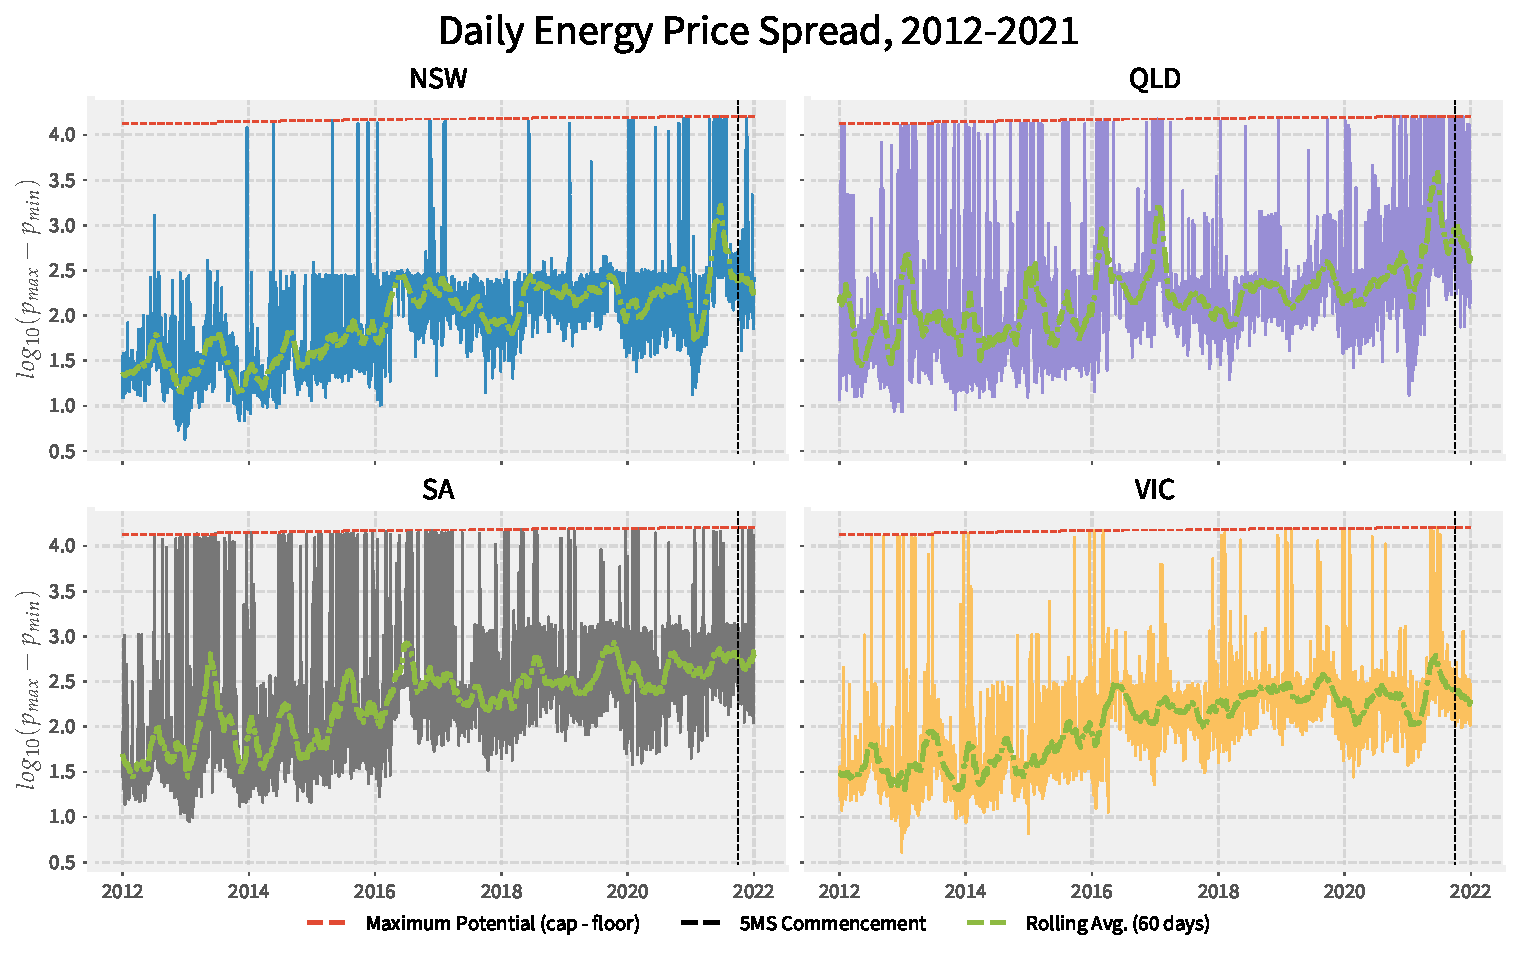
\includegraphics{source/figures/historical_daily_price_spreads.pdf}
\caption[Daily price spread in all mainland NEM regions from 2012 to the
end of 2021]{Common logarithm of the daily price spread (where
\(p_{max}\) and \(p_{min}\) are the maximum and minimum price for any
given day, respectively) in all mainland NEM regions (i.e.~excluding
TAS, which is connected to mainland Australia via a high voltage DC
transmission line) from 2012 to the end of 2021. The maximum potential
spread (dashed red line) is the difference between the market price cap
(revised each Australian financial year) and the fixed market price
floor (-1000 AUD/MW/hr). The dashed vertical black line denotes the
commencement of 5 minute settlement in the NEM. Price data were obtained
using \texttt{NEMOSIS}
(\protect\hyperlink{ref-gormanNEMOSISNEMOpen2018}{Gorman et al., 2018}).
This plot was generated using \texttt{matplotlib}
(\protect\hyperlink{ref-hunterMatplotlib2DGraphics2007}{Hunter,
2007}).}\label{fig:nem_daily_price_spreads}
}
\end{figure}

\hypertarget{sec:info-case_study}{%
\section{Pre-dispatch and its impact on storage scheduling in the
National Electricity Market}\label{sec:info-case_study}}

\hypertarget{sec:info-case_study-price_forecast_errors}{%
\subsection{Pre-dispatch price forecast
errors}\label{sec:info-case_study-price_forecast_errors}}

Aside from what appears to be anomalous outcomes for some months in 2016
(one of which is likely related to the SA system black that year),
Figure~\ref{fig:nem_historical_price_forecast_errors} shows that there
were relatively few significant pre-dispatch price forecast errors
(i.e.~errors with magnitude \(\geq\) 300 AUD/MW/hr)\footnote{300
  AUD/MW/hr corresponds to the traditional strike price of ``cap
  contracts''. These are a type of call option traded in the NEM's
  forward markets that, at the cost of a premium paid to the contract
  seller, enables contract purchasers (typically electricity retailers)
  to cap the market exposure of the contracted volume at the strike
  price.} in the NEM from 2012 to the end of 2017. However, price
forecast errors have increased in frequency since 2018 in the day-ahead
timeframe, and since 2019 for forecasts published up to 2 hours and 15
minutes ahead of delivery. The rise in price forecast errors consists
not only of a greater number of negative price errors (red), which are
an expected outcome of the pre-dispatch process (i.e.~MPs increase
resource availability in response to a high price forecast and
subsequently depress the cleared price), but also positive errors, which
appear to constitute a large portion of the errors occurring within 15
minutes of delivery. Positive errors this close to delivery are
particularly concerning to MPs because they may lead to missed
opportunities or, if MPs are scheduling ESR charging or have sold
forward contracts that their resources are not positioned to defend,
unexpected costs. There does not appear to be a clear link between the
occurrence of a major system or market event and a greater number of
errors -- there were a large number of errors following a system black
event in SA in 2016 and the explosion of a QLD coal unit in 2021, but
lulls in errors also followed the retirement of a large VIC coal plant
in 2017 and a double-separation event in 2018.

\begin{figure}
\hypertarget{fig:nem_historical_price_forecast_errors}{%
\centering
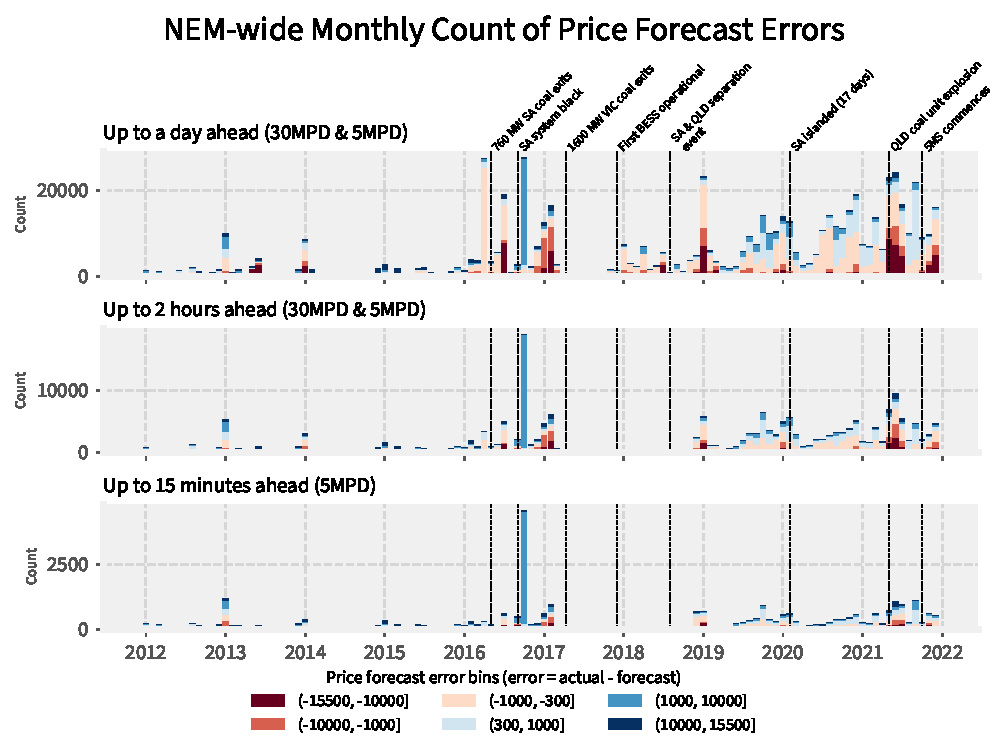
\includegraphics{source/figures/price_errors_nemwide_2012_2021.pdf}
\caption[Counts of NEM-wide price forecast errors, binned by direction
and magnitude, for each month from 2012 to 2021]{NEM-wide (i.e.~all
regions) monthly price forecast error counts binned by error direction
and magnitude (excluding -300 AUD/MW/hr \(<\) errors \(\leq\) 300
AUD/MW/hr ) for forecasts made up to 24 hours (top, using forecast data
from 30MPD and 5MPD), 2 hours (middle, using forecast data from 30MPD
and 5MPD) and 15 minutes (bottom, using forecast data from 5MPD) ahead
of delivery. The dashed and annotated black lines denote major system
events and market changes in the NEM. Pre-dispatch price forecasts data
were obtained using \texttt{NEMSEER}
(\protect\hyperlink{ref-prakashNEMSEERPythonPackage2023}{Prakash et al.,
2023b}), and actual market price data were obtained using
\texttt{NEMOSIS}
(\protect\hyperlink{ref-gormanNEMOSISNEMOpen2018}{Gorman et al., 2018}).
Errors for each forecasted interval were calculated following the
omission of the two 30MPD forecasts that overlap with the 5MPD forecast
horizon (refer to the research data for this article for further details
and source code). This plot was generated using \texttt{matplotlib}
(\protect\hyperlink{ref-hunterMatplotlib2DGraphics2007}{Hunter,
2007}).}\label{fig:nem_historical_price_forecast_errors}
}
\end{figure}

Flexible resources such as BESSs, hydro and VRE are able to adapt to
changing conditions so long as their primary energy source is available
and the market information relevant to their participation is published.
To better ascertain whether flexible resources might also be affected by
price forecast errors, we examine errors from the last available
pre-dispatch price forecast (i.e.~from the last P5MIN iteration, which
is nominally run 5 minutes before delivery).
Figure~\ref{fig:nsw_5min_price_demand_errors_2021} shows that for NSW in
2021, there were some intervals in which the last available price
forecast was different from the actual dispatch price by 10,000--15,000
AUD/MW/hr. Price forecast swings of this magnitude could have a
significant impact on inflexible and flexible resource alike, and are
possible with only small changes in supply or demand since resource
offers and aggregate supply curves in the NEM typically resemble
hockey-sticks
(\protect\hyperlink{ref-energysynapseDemandResponseNational2020}{Energy
Synapse, 2020};
\protect\hyperlink{ref-hurlbutProtectingMarketHockey2004}{Hurlbut et
al., 2004}). Factors that modify available supply, rather than demand,
between the last 5MPD run and actual dispatch are likely to be
responsible for these large swings as many of the significant price
errors in Figure~\ref{fig:nsw_5min_price_demand_errors_2021} occurred
when demand forecast errors were close to zero. Because sudden outages
are only occasional and AEMO regularly monitors pre-dispatch constraint
accuracy to check if improvements to their formulation can be made
(\protect\hyperlink{ref-australianenergymarketoperatorMonthlyConstraintReport2023}{Australian
Energy Market Operator, 2023c}), we conjecture that MP rebidding is a
major contributing factor to the large price forecast swings in
Figure~\ref{fig:nsw_5min_price_demand_errors_2021}. In the next section,
we analyse trends in MP rebidding and propose a hypothesis that links
rebidding activity to the rise in price forecast errors in the NEM.

\begin{figure}
\hypertarget{fig:nsw_5min_price_demand_errors_2021}{%
\centering
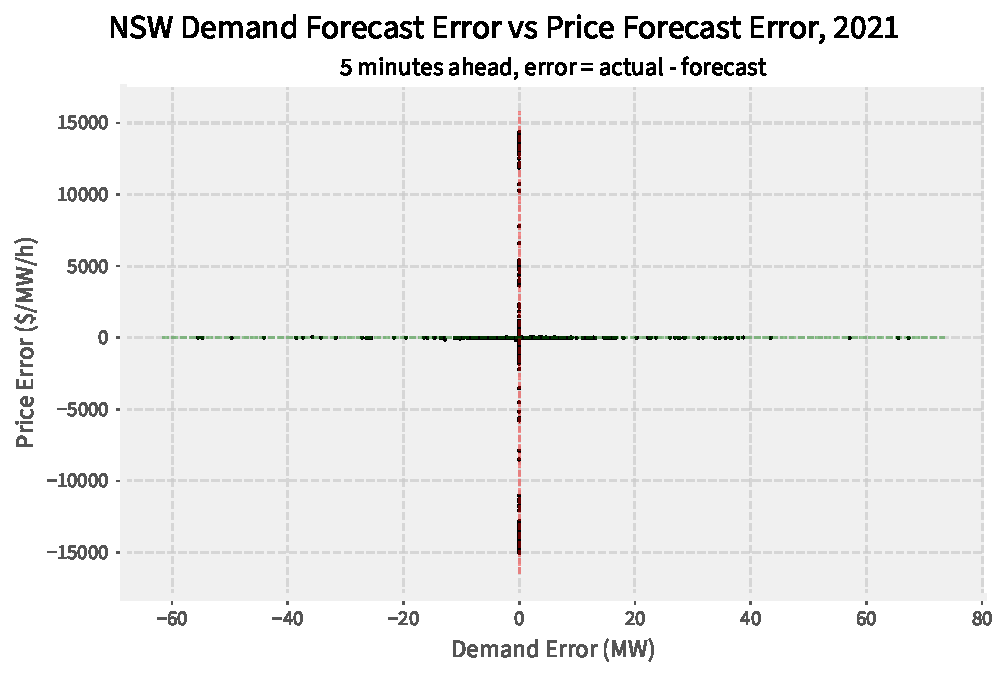
\includegraphics{source/figures/NSW_demand_price_forecast_errors_300ahead_2021.pdf}
\caption[Demand vs price forecast errors from the last 5MPD run for NSW,
2021]{Demand forecast error plotted against the price forecast error for
the NSW region in 2021. Each point in the scatter plot corresponds to
errors calculated from the forecasts in the last 5MPD run for each
dispatch interval (nominally run 5 minutes prior to delivery, but
published between 4.5 minutes and 3 minutes prior to delivery
(\protect\hyperlink{ref-mcardleFileCreationTimes2022}{McArdle, 2022})).
Source: \texttt{NEMSEER} documentation
(\protect\hyperlink{ref-prakashEnergyPriceConvergence2023}{Prakash,
2023b}), using data obtained using \texttt{NEMSEER}
(\protect\hyperlink{ref-prakashNEMSEERPythonPackage2023}{Prakash et al.,
2023b}) and \texttt{NEMOSIS}
(\protect\hyperlink{ref-gormanNEMOSISNEMOpen2018}{Gorman et al., 2018}).
This plot was generated using \texttt{matplotlib}
(\protect\hyperlink{ref-hunterMatplotlib2DGraphics2007}{Hunter,
2007}).}\label{fig:nsw_5min_price_demand_errors_2021}
}
\end{figure}

\hypertarget{sec:info-case_study-price_forecast_errors-bidding_analysis}{%
\subsubsection{A rise in rebidding:
autobidders?}\label{sec:info-case_study-price_forecast_errors-bidding_analysis}}

Using data zipfile size as a proxy for the total number of bids, offers
and rebids (which we will collectively refer to as \emph{rebids} hereon
for the sake of brevity), Figure~\ref{fig:bid_file_size_2012_2022} shows
a gradual increase in the number of rebids beginning in 2018, which
roughly coincides with the NEM's first grid-scale BESS starting to
participate in dispatch, followed by a more dramatic increase starting
in 2021. Whilst 5MS-related changes likely contributed to the rise in
rebidding in 2021, the number of rebids has continued to steadily
increase as of the end of 2022. We surmise that this sustained rise in
rebidding activity is a result of resources increasingly being
commissioned with or adopting automated bidding systems (or
\emph{autobidders}) that can rapidly rebid
(\protect\hyperlink{ref-mcardleRiseAutobidder2021}{McArdle, 2021b}).

\begin{figure}
\hypertarget{fig:bid_file_size_2012_2022}{%
\centering
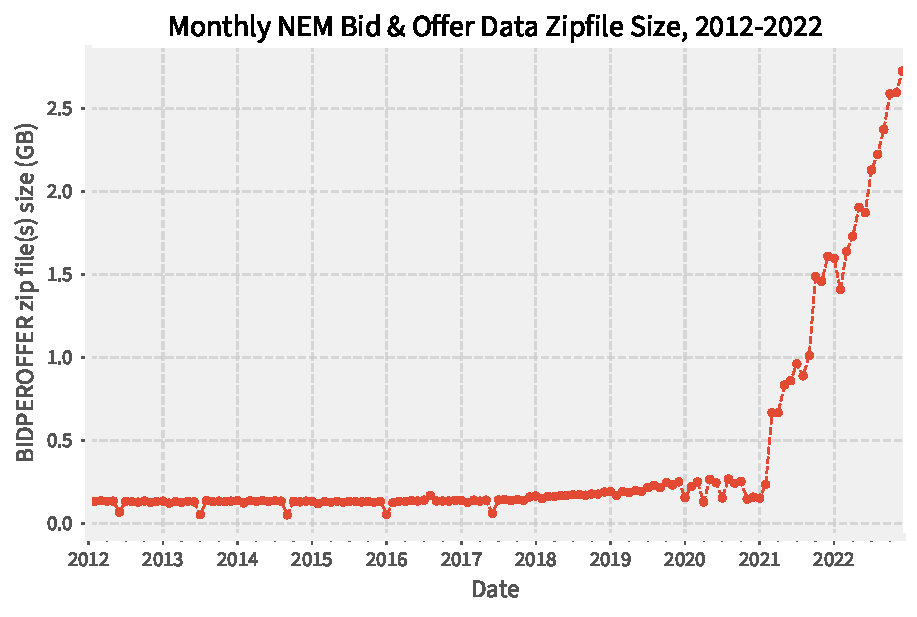
\includegraphics{source/figures/monthly_bidding_data_size_2012_2023.pdf}
\caption[Monthly NEM bid and offer data zipfile size from 2012 to
2022]{File sizes of monthly NEM bid and offer data zipfiles from 2012 to
2022 scraped from AEMO's monthly data archive
(\protect\hyperlink{ref-australianenergymarketoperatorElectricityDataModel2023}{Australian
Energy Market Operator, 2023d}). The zipfile for each month consists of
a single CSV with one AEMO data table (BIDPEROFFER) that contains
quantity bid and offer data (including rebids). As such, zipfile size is
a suitable proxy for the size of the underlying data and thus the number
of bids, offers and rebids. Two 5MS-related changes were accompanied by
spikes in bid and offer data zipfile size. The first is indicated by the
blue dashed line, which denotes when MPs were able to start submitting
the quantity component of their bids and offers for each 5-minute
dispatch interval (rather than each 30 minute interval) for the next
trading day. The second, denoted by the purple dashed line, denotes the
commencement of 5MS. This plot was generated using \texttt{matplotlib}
(\protect\hyperlink{ref-hunterMatplotlib2DGraphics2007}{Hunter,
2007}).}\label{fig:bid_file_size_2012_2022}
}
\end{figure}

To better understand which technologies are driving rebidding activity,
we calculated the percentage of rebids from each technology type in June
of every year from 2013 to 2021\footnote{The ramp rate used in dispatch
  by AEMO is the lesser of a telemetered rate or a ramp rate submitted
  in a resource's offer for energy, and was obtained using NEMOSIS
  (\protect\hyperlink{ref-gormanNEMOSISNEMOpen2018}{Gorman et al.,
  2018}).}. Figure~\ref{fig:share_rebids_june_2013_2021} shows that
rebids in June have grown considerably; there were \textasciitilde1--3
million rebids in June in 2013--2018, but this increased to
approximately 4.5 million rebids in 2020 and 46 million rebids in 2021.
Though conventional resources (especially hydro) were still responsible
for a large share of the increased rebidding activity in June 2021, BESS
and wind resources overtook coal and gas-fired power station in the
quantity of rebids submitted and BESS and VRE together accounted for
approximately 35\% of all rebids in June in 2021. This figure increases
to just over 40\% of all rebids if we include other newer market
entrants such as demand response and virtual power plant aggregators. It
is worth highlighting that BESS resources in particular are playing an
outsized role in rebidding; over 80 wind farms and 60 open-cycle gas
turbine units accounted for approximately 15\% and 9\% of all rebids in
June 2021, respectively, compared to only 12 BESS plant accounting for
\textasciitilde13\%\footnote{For all conventional resources, the
  distribution of offer prices resembles ``hockey-stick'' offer curves
  that are common in the NEM
  (\protect\hyperlink{ref-energysynapseDemandResponseNational2020}{Energy
  Synapse, 2020}) and in other electricity markets
  (\protect\hyperlink{ref-hurlbutProtectingMarketHockey2004}{Hurlbut et
  al., 2004}). Moreover, for most peaking conventional resources, energy
  is offered at or just above the strike price of cap options/futures
  (300 AUD/MWh).}.

Though we cannot make definitive conclusions, we surmise that the
significant increase in the number of rebids and the greater role of
newer market entrants in rebidding can be partially attributed to the
growing use of autobidders in the NEM. Autobidders are typically
integrated with BESS market participation control algorithms, and VRE
resources are increasingly using them to manage the various complexities
of market participation
(\protect\hyperlink{ref-mcardleRiseAutobidder2021}{McArdle, 2021b}).
Furthermore, we propose that the rise in pre-dispatch price forecast
errors, be they some time ahead of delivery or a sudden divergence close
to real-time, could at least be partially explained by greater rebidding
activity. MPs could be inducing large price forecast changes between
pre-dispatch runs, or between pre-dispatch and dispatch itself (e.g.
Figure~\ref{fig:nsw_5min_price_demand_errors_2021}), by regularly and
rapidly shifting supply availability through rebids -- a participation
strategy that is enabled by resource flexibility and facilitated by the
use of autobidders. In the next section, we shift focus from analysing
pre-dispatch price forecast errors to assessing their impact on the
arbitrage revenues of various BESS ESRs.

\begin{figure}
\hypertarget{fig:share_rebids_june_2013_2021}{%
\centering
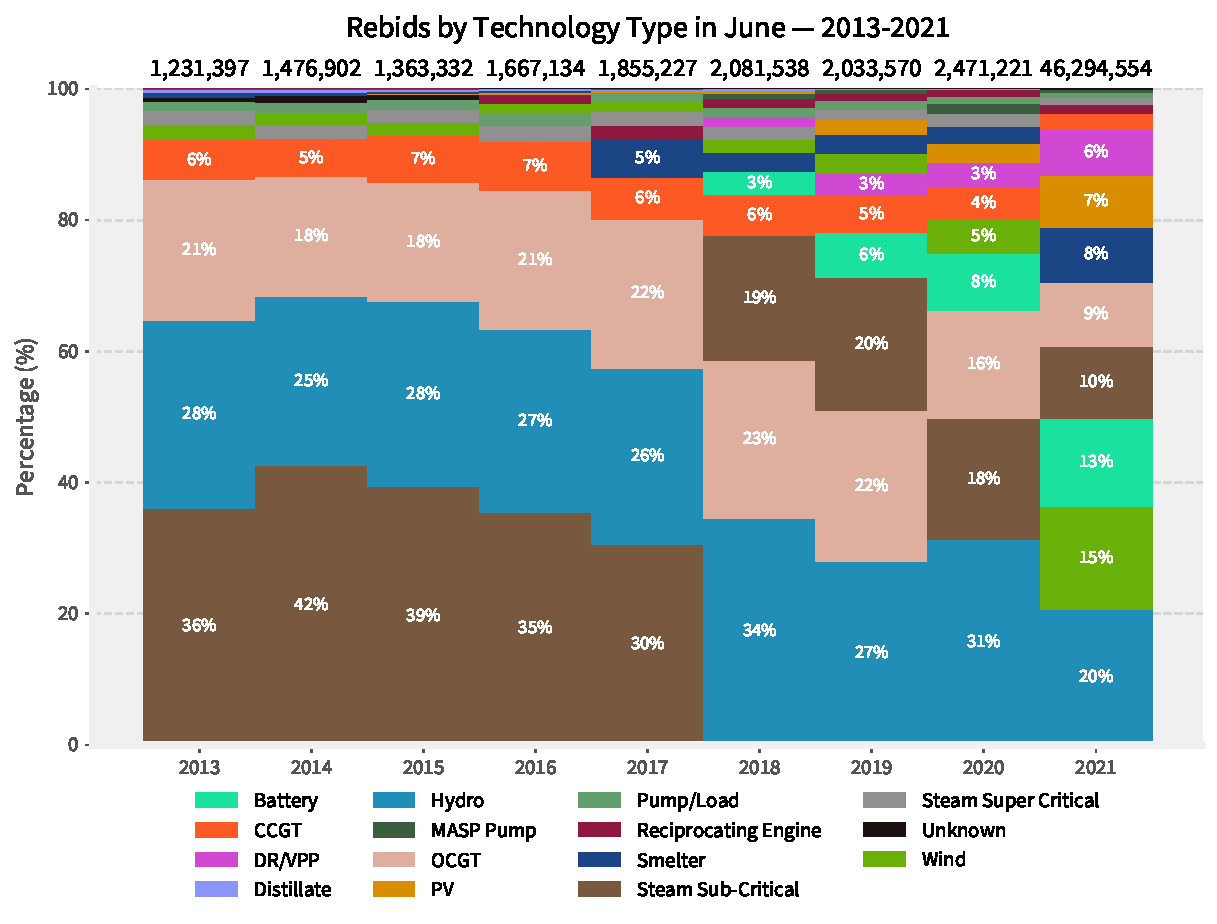
\includegraphics{source/figures/rebids_june_share_by_tech_2013_2021.pdf}
\caption[Share of rebids by technology type in June from 2013 to
2021]{Share of all rebids by technology type submitted in June for every
year from 2013 to 2021. The number at the top of each column is the
total number of rebids made in June of that year. June was selected
because it was this month in 2021 that saw the highest occurrence of
significant price forecast errors in several NEM regions across a range
of ahead times for half-hourly dispatch intervals (see Prakash
(\protect\hyperlink{ref-prakashEnergyPriceConvergence2023}{2023b})).
OCGT refers to open cycle gas turbines, CCGT refers to combined cycle
gas turbines and DR/VPP includes demand response and virtual power
plants, the latter of which has predominantly referred to aggregated
distributed BESS resources to date. Smelter refers to several existing
and now decommissioned aluminium smelters, and steam technologies
include resources with both coal-fired and gas-fired boilers. Rebid data
were obtained from Nemweb
(\protect\hyperlink{ref-australianenergymarketoperatorNemwebMarketData2023}{Australian
Energy Market Operator, 2023e}) using the open-source
\texttt{AEMO\ Monthly\ Data\ Archive\ Tool}
(\protect\hyperlink{ref-prakashAEMOMonthlyData2023}{Prakash, 2023a}).
This plot was generated using \texttt{matplotlib}
(\protect\hyperlink{ref-hunterMatplotlib2DGraphics2007}{Hunter,
2007}).}\label{fig:share_rebids_june_2013_2021}
}
\end{figure}

\hypertarget{sec:info-case_study-bess_simulations}{%
\subsection{Energy storage scheduling using pre-dispatch price
forecasts}\label{sec:info-case_study-bess_simulations}}

Through an optimisation modelling framework, we test the degree to which
information quality affects the annual arbitrage revenues of 100 MW
BESSs with different storage durations, scheduling optimisation
objectives and scheduling lookaheads. We do so for the NSW market
region, which provides an interesting case study given its relatively
low price volatility historically
(Figure~\ref{fig:nem_daily_price_spreads}) yet recent experience with
sudden and significant price forecast swings (refer to Prakash
(\protect\hyperlink{ref-prakashEnergyPriceConvergence2023}{2023b}) and
Figure~\ref{fig:nsw_5min_price_demand_errors_2021}).

\hypertarget{sec:info-case_study-bess_simulations-method}{%
\subsubsection{Methodology}\label{sec:info-case_study-bess_simulations-method}}

\hypertarget{sec:info-case_study-bess_simulations-method-price_data}{%
\paragraph{Price
data}\label{sec:info-case_study-bess_simulations-method-price_data}}

Two types of price data for the NSW market region from 2021 were used in
this study:

\begin{enumerate}
\def\labelenumi{\arabic{enumi}.}
\tightlist
\item
  Actual price data obtained using \texttt{NEMOSIS} to represent
  \emph{perfect} price information
  (\protect\hyperlink{ref-gormanNEMOSISNEMOpen2018}{Gorman et al.,
  2018}); and
\item
  Price forecast data generated from processing 30MPD and 5MPD price
  forecasts obtained using \texttt{NEMSEER}
  (\protect\hyperlink{ref-prakashNEMSEERPythonPackage2023}{Prakash et
  al., 2023b}) in three steps. Firstly, because 30MPD only produces
  forecasts with half-hourly resolution, 30MPD price forecasts were
  imputed using the next observation carried backwards (i.e.~forecasted
  price at 13:30 is applied to intervals ending at 13:25, 13:20, \ldots,
  13:05). This reflects a typical interpretation of a 30MPD forecast.
  Secondly, because 30MPD is only run every half hour, the latest set of
  30MPD forecasts were carried forward (i.e.~set of forecasts generated
  at 13:30 are also used in intervals ending at 13:35,
  13:40,\ldots,13:55). Finally, the 30MPD forecasts for dispatch
  intervals within one hour of delivery were removed in favour of 5MPD
  price forecasts at 5-minute resolution. Together, these processing
  steps produced forecasts (or \emph{imperfect information}) for each
  dispatch interval with 5-minute resolution up to 15 hours out from
  delivery\footnote{30MPD produces forecasts until the end of the latest
    trading day for which offer and bid price band submission has
    closed. For example, the 1300 run on day D, the 0800 run on day D+1
    and the 1200 run on day D+1 will all forecast out until 0400 on day
    D+2 (trading days in the NEM commence at 0400). The longest
    lookahead for which all dispatch intervals have a 30MPD forecast is
    16 hours
    (\protect\hyperlink{ref-prakashLookingPredispatchDemand2023}{Prakash,
    2023c}).}.
\end{enumerate}

\hypertarget{schedules}{%
\paragraph{Schedules}\label{schedules}}

Three year-long arbitrage schedules consisting of decisions to charge,
discharge or idle were generated for each modelled BESS: one using a
perfect foresight model, in which BESS operation is optimised across the
entire year using actual price data in a single \emph{step}, and two
(one with actual and one with forecast price data) using a receding
horizon optimal control (RHOC) simulation
(Figure~\ref{fig:bess_schedules}). The RHOC simulations consisted of
\emph{steps} every 5 minutes in which BESS operation is optimised for
the duration of the lookahead horizon with actual or forecast price
data, but only the action for the next dispatch interval is considered
to be \emph{binding} and is thus retained as a scheduling decision that
affects the BESS's state of charge. Successive steps were taken until a
schedule for the entire year of 2021 was produced. Each step required
optimising one of the mixed-integer linear program (MILP) formulations
described in
Section~\ref{sec:info-case_study-bess_simulations-method-sensitivity_analysis},
all of which used a single binary variable for each interval in the
forecast horizon to prevent the BESS from simultaneously charging and
discharging in the same dispatch interval
(\protect\hyperlink{ref-shafieeEconomicAssessmentPricemaker2016}{Shafiee
et al., 2016};
\protect\hyperlink{ref-wangOptimalSchedulingEnergy2017}{Wang et al.,
2017};
\protect\hyperlink{ref-yurdakulRiskAverseSelfSchedulingStorage2023}{Ogun
Yurdakul and Billimoria, 2023}).

\begin{figure}
\hypertarget{fig:bess_schedules}{%
\centering
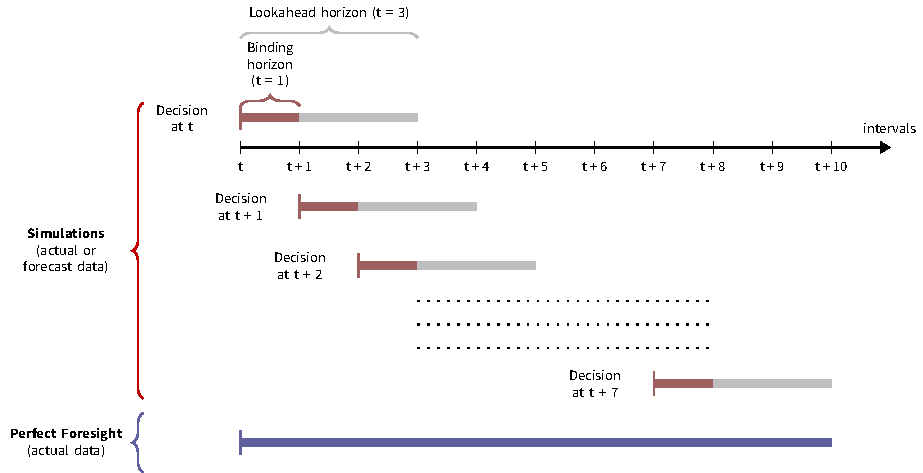
\includegraphics{source/figures/storage_simulations.pdf}
\caption[The study\textquotesingle s methodology for scheduling BESS
under imperfect and perfect foresight]{The study's scheduling
methodologies applied across 10 dispatch intervals (50 minutes). The top
of the figure (within the red brace) corresponds to the RHOC simulation
methodology. The scheduler optimises successive steps, each with a
lookahead horizon length of 3 intervals or 15 minutes, and binds the
first action of each step (red horizontal bars) to create a simulated
BESS schedule. The bottom of the figure (within the blue brace)
corresponds to the perfect foresight methodology. The perfect foresight
scheduler optimises a single step that looks over the entire study
period to produce a perfect foresight BESS
schedule.}\label{fig:bess_schedules}
}
\end{figure}

The perfect foresight model and RHOC simulations were implemented in
Julia (\protect\hyperlink{ref-bezansonJuliaFreshApproach2017}{Bezanson
et al., 2017}). The MILP formulations were written in the \texttt{JuMP}
modelling language
(\protect\hyperlink{ref-lubinJuMPRecentImprovements2023}{Lubin et al.,
2023}) and solved using \texttt{HiGHs}
(\protect\hyperlink{ref-huangfuParallelizingDualRevised2018}{Huangfu and
Hall, 2018}) with a 1\% relative MIP gap tolerance and a 30 second time
limit. These solver options were chosen such that solutions of a
reasonable quality were attained whilst ensuring that the time required
to solve more than 100,000 successive steps for a year-long schedule
would not be prohibitive. Figures were generated using \texttt{Makie.jl}
(\protect\hyperlink{ref-danischMakieJlFlexible2021}{Danisch and
Krumbiegel, 2021}). All of the aforementioned packages and this study's
source code
(\protect\hyperlink{ref-prakashNEMStorageUnderUncertainty2023}{Prakash,
2023d}) are open-source and freely-available.

\hypertarget{sec:info-case_study-bess_simulations-method-sensitivity_analysis}{%
\paragraph{Sensitivity
analysis}\label{sec:info-case_study-bess_simulations-method-sensitivity_analysis}}

A sensitivity analysis was conducted to test the impact of information
quality (i.e.~perfect versus imperfect information) on the annual
arbitrage revenues of BESSs with different:

\begin{enumerate}
\def\labelenumi{\arabic{enumi}.}
\tightlist
\item
  \textbf{Storage durations}. These ranged from 15 minutes to 4 hours
  for a 100 MW BESS. This power capacity and the duration range tested
  are reflective of those of BESS resources that are currently
  participating in the NEM;
\item
  \textbf{Lookahead horizon lengths}. Each step involves optimising the
  BESS using actual or forecast price data for just the next dispatch
  interval (5 minutes) or as far as 15 hours (900 minutes) out; and
\item
  \textbf{Interpretations of arbitrage opportunities}. These are
  modelled via the optimisation problem \emph{formulations} described in
  Table~\ref{tbl:formulations}.
\end{enumerate}

\hypertarget{tbl:formulations}{}
\begin{longtable}[]{@{}
  >{\raggedright\arraybackslash}m{(\columnwidth - 4\tabcolsep) * \real{0.2016}}
  >{\raggedright\arraybackslash}m{(\columnwidth - 4\tabcolsep) * \real{0.5565}}
  >{\raggedright\arraybackslash}m{(\columnwidth - 4\tabcolsep) * \real{0.2339}}@{}}
\caption{\label{tbl:formulations}Optimisation problem formulations
simulated in this study.}\tabularnewline
\toprule\noalign{}
\begin{minipage}[b]{\linewidth}\raggedright
Name
\end{minipage} & \begin{minipage}[b]{\linewidth}\raggedright
Description
\end{minipage} & \begin{minipage}[b]{\linewidth}\raggedright
MILP Formulation
\end{minipage} \\
\midrule\noalign{}
\endfirsthead
\toprule\noalign{}
\begin{minipage}[b]{\linewidth}\raggedright
Name
\end{minipage} & \begin{minipage}[b]{\linewidth}\raggedright
Description
\end{minipage} & \begin{minipage}[b]{\linewidth}\raggedright
MILP Formulation
\end{minipage} \\
\midrule\noalign{}
\endhead
\bottomrule\noalign{}
\endlastfoot
\emph{Arbitrage} & Maximise arbitrage revenues over the lookahead
horizon subject to power, energy and charge state constraints. &
Appendix \ref{sec:appendix-milps-arb} \\
\emph{TP Penalty {[}AUD/MWh{]}} & As for \emph{Arbitrage}, but with a
penalty applied to BESS throughput (discharged energy) to model a MP
assessing arbitrage revenue potential against the cost of BESS cycle
degradation. The penalty is the capital cost of a BESS amortised across
a warrantied throughput lifetime, which was calculated using a cycle
rate (1 cycle per day) and warranty period (10 years) typical of many
existing BESS warranties
(\protect\hyperlink{ref-xuRoleModelingBattery2022}{Xu, 2022}). The BESS
capital costs used in this study ranged from 200,000 to 800,000 AUD/MWh.
This range encompasses the capital cost assumptions for grid-scale BESS
of various storage durations that AEMO have used in their capacity
expansion modelling
(\protect\hyperlink{ref-australianenergymarketoperator2022ISPInputs2022}{Australian
Energy Market Operator, 2022f}). The number in the square brackets that
follows the formulation name denotes the BESS capital cost used in the
penalty (in AUD/MWh). & Appendix \ref{sec:appendix-milps-arbpen} \\
\emph{Discounting + TP Pen. {[}Discount function{]}} & As for \emph{TP
Penalty {[}600,000 AUD/MWh{]}} (mid-range BESS capital cost), but with
future prices discounted based on a discount function and discount rate.
This models a MP incorporating the belief that forecasts should improve
closer to real-time into the BESS scheduling process. Two discount
functions were tested: the commonly-used exponential discount function
(\emph{Exp}) and a hyperbolic discount function (\emph{Hyp}). We outline
the rationale for choosing these discount functions and describe the
methodology used to derive discount rates in Appendix
\ref{sec:appendix-discounting}. & Appendix
\ref{sec:appendix-milps-arbdisc} \\
\end{longtable}

\hypertarget{sec:info-case_study-bess_simulations-method-assumptions}{%
\paragraph{Assumptions and
limitations}\label{sec:info-case_study-bess_simulations-method-assumptions}}

Below, we outline the simplifying assumptions made by the study with
regards to BESS dispatch and market participation. We discuss
assumptions related to the BESS's operating characteristics in Appendix
\ref{sec:appendix-milps-assumptions}.

\begin{itemize}
\tightlist
\item
  The BESS does not participate in FCAS or provide other system
  services. Modelling these would likely reduce the power and/or energy
  capacity available for arbitrage and also require the scheduler to
  consider FCAS price forecasts.
\item
  We optimise the BESS for dispatch decisions, but MPs would actually
  optimise their rebids. In theory, appropriately structuring a BESS's
  price-quantity bands should mean that it only participates when it is
  commercially beneficial to do so whilst minimising or altogether
  avoiding losses in the event of sudden price forecast swings. In
  practice, many BESS across the NEM appear to be sacrificing some
  arbitrage upside by pursuing loss-averse bidding strategies. These
  entail a BESS bidding a large portion of its capacity into higher
  price bands to avoid being dispatched if low or moderate prices
  eventuate, and only rebidding this capacity into lower price bands
  when participation is perceived to be favourable
  (Figure~\ref{fig:nem_bess_bidding}). Though at least some BESSs no
  longer have this ``all-or-nothing'' approach to loss-averse bidding
  (compare 2021 and 2023 in Figure~\ref{fig:nem_bess_bidding}), there
  may be instances in which forecasts fail to predict a moderate-to-high
  price and a BESS only partially captures or even completely misses a
  significant revenue opportunity.
\item
  The scheduling decisions made by the 100MW BESS assume that it is a
  ``small device'', i.e.~a price-taker. Given the hockey-stick shape of
  the NEM's aggregate supply curves, this assumption is likely to hold
  for lower prices. However, the BESS could play a role in shaping
  higher prices, e.g.~shifting offered quantities to prevent prices from
  being depressed or to exercise market power. Doing so successfully
  would not only rely on accurate price forecasts, but also a good
  understanding of the BESS's own market power.
\item
  The BESS maintains a dispatch target for the entire interval instead
  of ramping linearly between its last and next dispatch target -- a
  requirement in the NEM
  (\protect\hyperlink{ref-australianenergymarketoperatorDispatchStandardOperating2019}{Australian
  Energy Market Operator, 2021d}).
\item
  BESS dispatch is not restricted by constraints in the NEM's dispatch
  engine.
\item
  The market is settled for each dispatch interval, with the BESS being
  paid or charged the corresponding spot price for the NSW region. In
  reality, the regional spot price would be adjusted by the marginal
  loss factor of the BESS
  (\protect\hyperlink{ref-aemoTreatmentLossFactors2012}{Australian
  Energy Market Operator, 2012b}).
\end{itemize}

\begin{figure}
\hypertarget{fig:nem_bess_bidding}{%
\centering
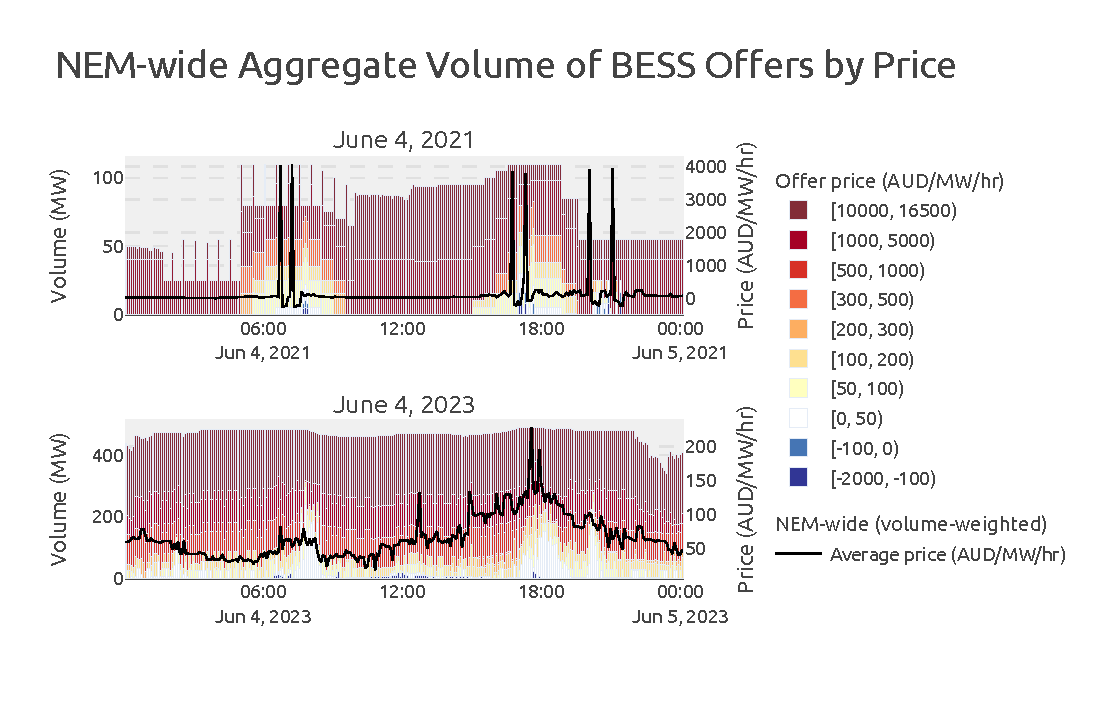
\includegraphics{source/figures/aggregate_bess_bidding_0406_2021_2023.pdf}
\caption[Aggregated final BESS offers on June 4 2021 and June 4
2023]{Final aggregate BESS offers adjusted by resource availability and
binned by offer price, and the NEM-wide volume weighted average prices
on June 4 2021 and June 4 2023. Note that BESS, like other resources in
the NEM, tend to shift capacity to lower price bands during periods of
high prices. While BESS capacity was predominantly offered in at 1000+
AUD/MW/hr between high price events in 2021, there was a higher degree
of quantity segmentation across 50 AUD/MW/hr+ price bands in 2023
(albeit with higher total offer volumes). Nevertheless, more than half
of the aggregate in-market BESS capacity was at times offered into the
market for at least 10,000 AUD/MW/hr on June 4 2023. Final offers were
obtained and processed using \texttt{nem-bidding-dashboard}
(\protect\hyperlink{ref-gormanNembiddingdashboard2023}{Gorman and
Chambers, 2023}). This plot was generated using \texttt{plotly}
(\protect\hyperlink{ref-plotlytechnologiesinc.CollaborativeDataScience2015}{Plotly
Technologies Inc., 2015}).}\label{fig:nem_bess_bidding}
}
\end{figure}

\hypertarget{values-of-perfect-information-and-foresight}{%
\paragraph{Values of perfect information and
foresight}\label{values-of-perfect-information-and-foresight}}

Inspired by metrics for evaluating solutions obtained from optimisation
under uncertainty
(\protect\hyperlink{ref-roaldPowerSystemsOptimization2023}{Roald et al.,
2023}), we compute two quantities to separate the impact of imperfect
information from that of myopic lookaheads and sub-optimal
decision-making:

\begin{enumerate}
\def\labelenumi{\arabic{enumi}.}
\tightlist
\item
  \emph{Value of perfect information} (VPI), which is obtained by
  expressing the additional annual revenue earned with access to actual
  price information, rather than forecast prices, for \emph{each RHOC
  simulation step} as a percentage of the perfect foresight annual
  revenue:
\end{enumerate}

\[\textrm{VPI} = \frac{\textrm{Revenue}_{\textrm{Actual}} - \textrm{Revenue}_{\textrm{Forecast}}}{\textrm{Revenue}_{\textrm{Perfect foresight}}}\]

\begin{enumerate}
\def\labelenumi{\arabic{enumi}.}
\setcounter{enumi}{1}
\tightlist
\item
  \emph{Value of perfect foresight} (VPF), which is obtained by
  expressing the additional annual revenue earned with access to actual
  price information for the \emph{entire year} as a percentage of the
  perfect foresight annual revenue:
\end{enumerate}

\[\textrm{VPF} = \frac{\textrm{Revenue}_{\textrm{Perfect foresight}} - \textrm{Revenue}_{\textrm{Forecast}}}{\textrm{Revenue}_{\textrm{Perfect foresight}}}\]

If \(\textrm{VPF} \approx \textrm{VPI}\), then information quality
accounts for most of the lost revenue potential. Otherwise if
\(\textrm{VPF} > \textrm{VPI}\), then other changes, such as increasing
the scheduling lookahead, are required alongside better information to
recoup lost revenue potential.

\hypertarget{sec:info-case_study-bess_simulations-method-results}{%
\subsubsection{Results}\label{sec:info-case_study-bess_simulations-method-results}}

Using pre-dispatch price forecasts can have a significant impact on BESS
annual arbitrage revenues. Though a BESS scheduled with perfect
information but a shorter lookahead horizon length of 1 hour can make
some minor detrimental decisions (left plot in
Figure~\ref{fig:bess_price_revenue}), using price forecasts can lead to
a BESS missing a larger number of revenue opportunities and sometimes
incurring significant costs as a consequence of charging during an
unanticipated price spike (right plot in
Figure~\ref{fig:bess_price_revenue}). Over the entire study year, using
undiscounted price forecasts across the longest lookahead horizon
reduced BESS arbitrage revenue potential by \textasciitilde15--20\% for
a 4 hour BESS, \textasciitilde40--43\% for a 1 hour BESS and as much as
\textasciitilde62--64\% for a 15 minute BESS (Figure~\ref{fig:vpi_vpf}).

\begin{figure}
\hypertarget{fig:bess_price_revenue}{%
\centering
\includegraphics{source/figures/NSW_100MW_100MWh_Revenue_Lookahead.pdf}
\caption[Revenue vs energy price for simulated BESSs with 1 hour storage
duration over the simulated year (2021)]{The revenue earned by a 100
MW/100 MWh BESS (scheduled using the \emph{Arbitrage} formulation)
plotted against the energy price in the same dispatch interval. Orange
points correspond to dispatch interval decisions made with a lookahead
horizon length of 15 hours and blue points correspond to dispatch
interval decisions made with a lookahead horizon length of 1 hour. Under
ideal operation, the points should form a ``tick'' shape -- more
negative prices should lead to greater revenues as the BESS charges, and
a higher price should lead to greater revenues as the BESS
discharges.}\label{fig:bess_price_revenue}
}
\end{figure}

\begin{figure}
\hypertarget{fig:vpi_vpf}{%
\centering
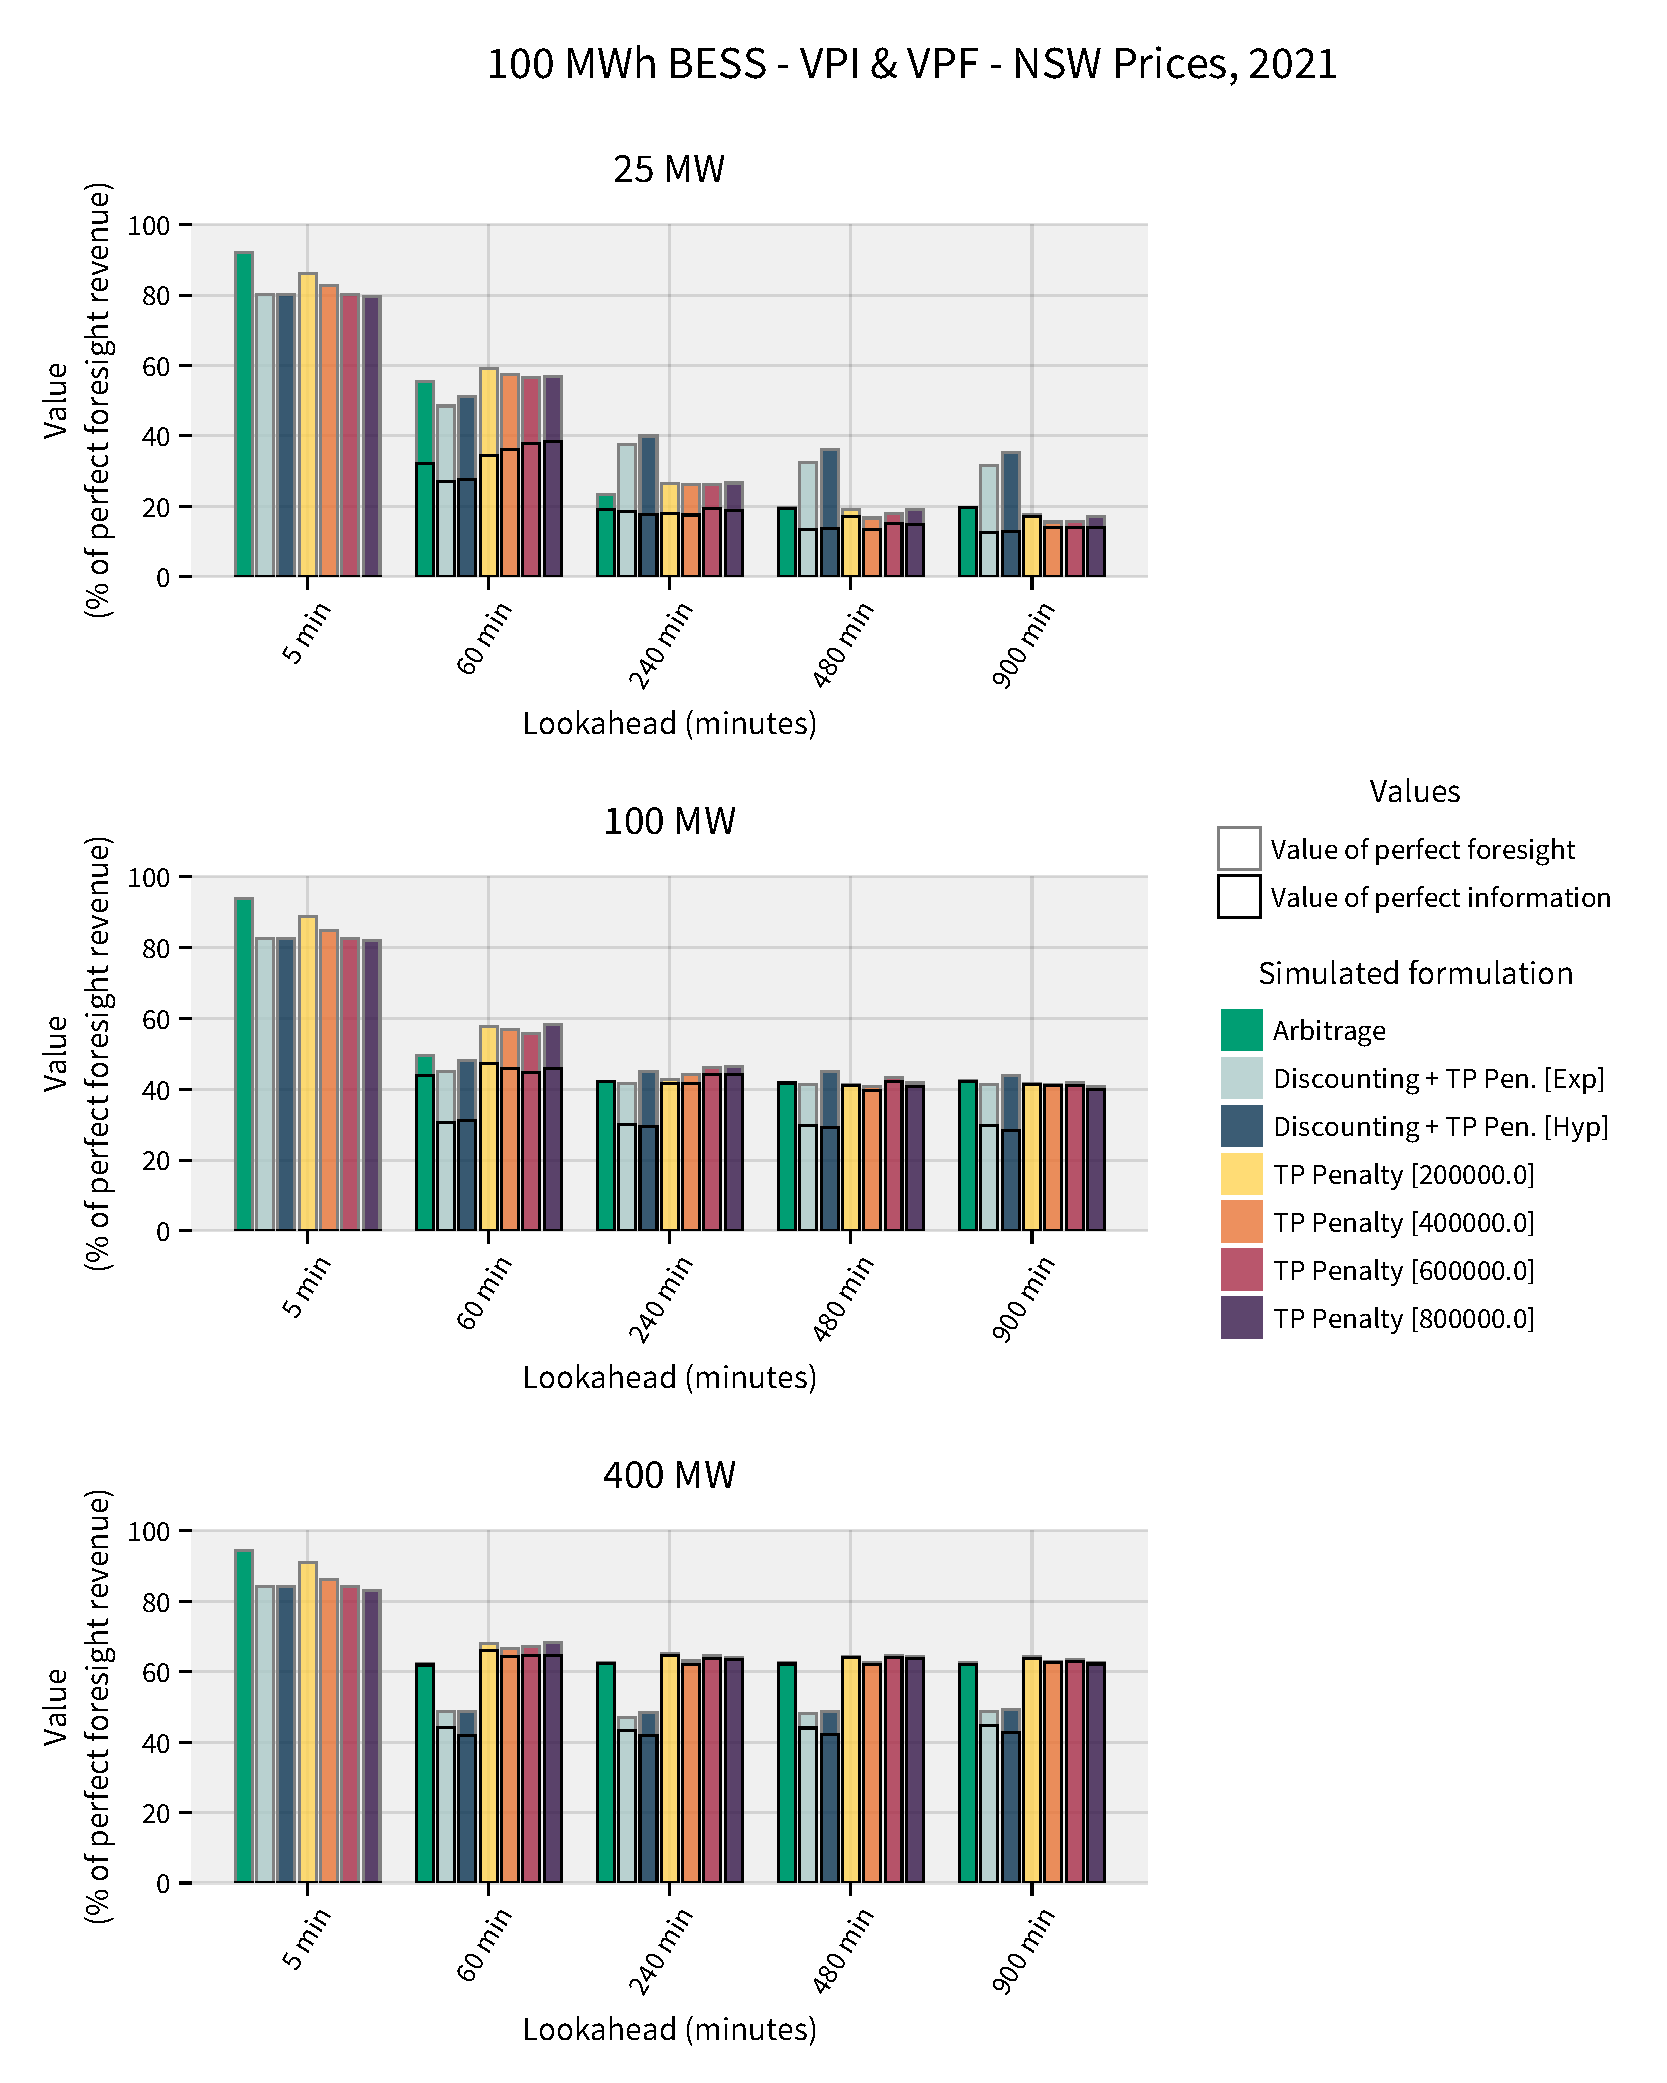
\includegraphics{source/figures/NSW_100_allformulations_vpi_vpf.pdf}
\caption[Value of perfect information and foresight for each simulated
BESS]{VPI (bars with black edges) and VPF (bars with grey edges) for
BESS with different storage durations (15 minutes to 4 hours across
subfigures from top to bottom), lookahead horizon lengths (5 minutes to
15 hours across the horizontal axis of each subfigure) and optimisation
formulations (different coloured bars, all described in
Table~\ref{tbl:formulations}). Note that for the BESSs with 5 minute
lookahead horizon lengths, the VPI bars are close to zero (i.e.~myopic
operation dominates lost revenue potential).}\label{fig:vpi_vpf}
}
\end{figure}

Despite the magnitude of the aforementioned revenue reductions, our
results also suggest that storage operators can reduce the impact of
imperfect information to varying degrees by:

\begin{enumerate}
\def\labelenumi{\arabic{enumi}.}
\item
  Scheduling using longer lookahead horizons. As demonstrated by the
  reduction in the difference between VPF and VPI from a 5 minute to 15
  hour lookahead for the 25 MW BESS, a long lookahead horizon is
  unsurprisingly important to longer duration storage. However, across
  most of the sensitivities tested in this study, our results suggest
  that most of this benefit can be captured with a lookahead horizon as
  short as 4 hours. This is because for undiscounted simulations,
  forecast quality accounts for most if not all of the lost revenue
  potential (i.e.~\(VPF \approx VPI\)) beyond 4 hours. Medium to
  longer-term operational planning is also important. Cycling
  constraints, such as those imposed by manufacturer warranties, may
  incentivise BESS operators to ``preserve'' cycles for the best
  opportunities (e.g.~May to August in this study, which is, as
  Figure~\ref{fig:bess_throughputs} shows, when the perfect foresight
  BESS was cycled the most).
\item
  Discounting price forecasts further into the future when scheduling
  BESS with sub-hourly storage durations. The exponential function
  slightly outperforms the hyperbolic function mostly likely due to the
  latter's heavier discounting price forecasts closer to real-time,
  which tend to be more accurate (see Appendix
  \ref{sec:appendix-discounting}). Using the discounting methods tested
  in this study leads to worse outcomes for the 4 hour BESS as
  longer-term arbitrage opportunities are devalued (e.g.~a cost to
  charge now is evaluated against a discounted future revenue earned
  from discharging).
\end{enumerate}

\begin{figure}
\hypertarget{fig:bess_throughputs}{%
\centering
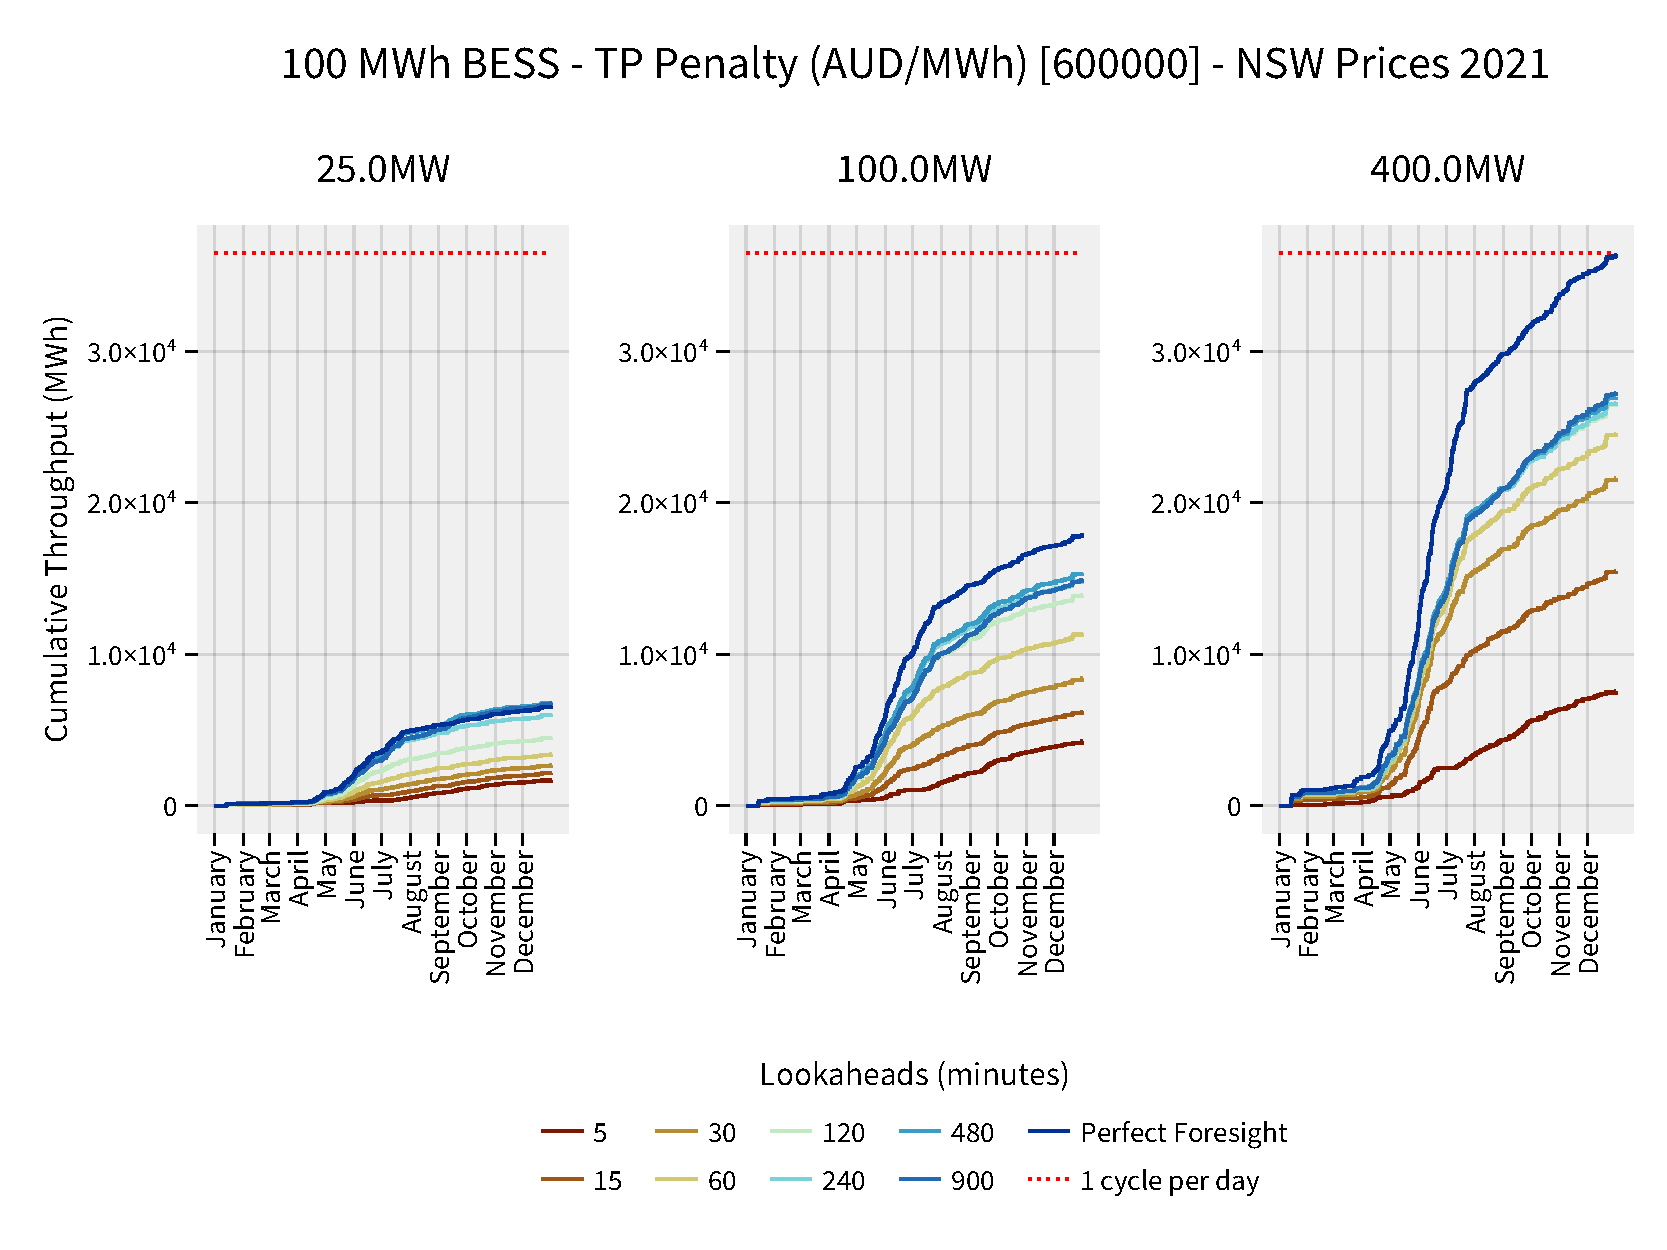
\includegraphics{source/figures/NSW_100_arbitrage_throughputpenalty_no_degradation_600000_throughputs.pdf}
\caption[Cumulative throughput of BESSs with 15 minutes, 1 hour and 4
hours of storage throughout the simulated year (2021)]{Cumulative
throughput (discharged energy) for BESSs with different storage
durations (15 minutes, 1 hour and 4 hours in the subfigures from left to
right) and different scheduling lookahead horizon lengths (different
coloured lines in each subfigure) in 2021. The dashed red line indicates
the end-of-year cumulative throughput of a 100 MWh BESS that is cycled
once per day.}\label{fig:bess_throughputs}
}
\end{figure}

\hypertarget{sec:info-discussion}{%
\section{Options for improving scheduling}\label{sec:info-discussion}}

The results from Section~\ref{sec:info-case_study-bess_simulations}
suggest that the increasing frequency and severity of price forecast
errors in the NEM's pre-dispatch processes could be hampering their
function as a scheduling coordination platform. In particular, flexible
resources such as ESRs can lose significant fractions of their potential
revenue to instances of sudden and extreme price divergence -- products
of the NEM's fast real-time market, its lenient bidding rules, common MP
bidding strategies and inelastic demand. In this section, we discuss
options for MPs to mitigate the impact of imperfect information, and
changes to centralised knowledge processes and market design that
policy-makers could implement to improve resource scheduling outcomes.

MPs need not solely rely on centralised knowledge processes given that
they can generate either their own point forecasts for use in
deterministic scheduling methods, or forecasted distributions of prices
(or price errors) for use in stochastic or robust scheduling methods
(discussed in Section~\ref{sec:info-context-esr-operation-information}).
However, in markets with blind auctions, producing private forecasts
requires using historical data that likely reflect past market dynamics
(\protect\hyperlink{ref-lagoForecastingDayaheadElectricity2021}{Lago et
al., 2021a}). In contrast, pre-dispatch is \emph{mechanistic} -- the
best-available forward-looking information, which includes forecasted
demand and constraints and the latest set of sealed bids and offers, is
used in a modified copy of the market clearing engine
(\protect\hyperlink{ref-trebbienUnderstandingElectricityPrices2023}{Trebbien
et al., 2023}). MPs desiring a balanced solution would ideally use both
private and pre-dispatch forecasts in their decision-making, as the
former may be more robust to ``noisy'' market processes whilst the
latter better reflects contemporaneous market dynamics and system
constraints. Beyond improving price forecast accuracy, MPs should
consider two scheduling changes that could improve market revenues.
Firstly, scheduling algorithm modifications (e.g.~as suggested in
Section~\ref{sec:info-case_study-bess_simulations-method-results},
longer lookaheads and the tested forecast discounting methods for ESRs
with short storage durations) may deliver material improvements whilst
being simple to implement. Secondly, rather than pursuing all-or-nothing
(Section~\ref{sec:info-case_study-bess_simulations-method-assumptions})
or hockey-stick bidding strategies, MPs could appropriately structure
their price-quantity bands to reflect costs and manage price risk.
However, doing so would require MPs to partially divulge otherwise
private information to the broader market and, for ESRs, could lead to
increased cycling.

Though there are risks associated with ``analytical monocultures'' in
which the ``wisdom of the crowd'' is replaced by shared beliefs and thus
correlated actions
(\protect\hyperlink{ref-bowlesRetrospectivesFriedrichHayek2017}{Bowles
et al., 2017}; \protect\hyperlink{ref-bronkHayekWisdomPrices2013}{Bronk,
2013}), improving the scheduling decision support offered by centralised
knowledge processes may be necessary to address existing information and
power asymmetries, and could become essential should policy-makers
pursue two-sided or hierarchical market architectures that enable
smaller consumer-owned energy resources to participate in real-time
markets (\protect\hyperlink{ref-hoganMarketDesignPractices2019}{Hogan,
2019}; \protect\hyperlink{ref-kristovTaleTwoVisions2016}{Kristov et al.,
2016}). One approach to improving decision support is to provide more
information to MPs. This could not only involve publishing additional
metrics (e.g.~forecast uncertainty measures or the regional aggregate
energy availability of energy-constrained resources)
(\protect\hyperlink{ref-australianenergymarketcommissionOperatingReserveMarket2023}{Australian
Energy Market Commission, 2023c}) but also implementing probabilistic or
interactive pre-dispatch engines that provide MPs with a broader
perspective of possible market outcomes than the pre-dispatch
sensitivities discussed in
Section~\ref{sec:info-context-nem-knowledge_processes}. Notwithstanding
the transparency benefits, the costs of increased information provision
could exceed its benefits if it has little effect on MP decision-making
due to greater complexity (e.g.~if pre-dispatch deviates from the
real-time market clearing algorithm) or the additional information is
not immediately decision-relevant. It could even have deleterious
effects should it provide information that reveals opportunities for
gaming or collusion to MPs
(\protect\hyperlink{ref-creativeenergyconsultingptyltdSchedulingAheadMarkets2020}{Creative
Energy Consulting Pty Ltd, 2020};
\protect\hyperlink{ref-vonderfehrTransparencyElectricityMarkets2013}{Von
Der Fehr, 2013}).

Another approach to improving the decision support offered by
centralised knowledge processes is to promote schedule and price
convergence. One low-regret option that might assist with convergence is
increasing the frequency at which pre-dispatch and PASA are published.
More frequent information provision may be particularly effective for a
future NEM that will likely consist of many flexible resources that can
rapidly respond to changing market conditions. However, this change's
feasibility is limited by the minimum solution times for these processes
and, more importantly, it does not reduce the likelihood of sudden and
extreme price forecast swings
(Section~\ref{sec:info-case_study-price_forecast_errors}). Addressing
these swings may require restricting rebidding since the freedom to
readily shift participation preferences frequently, dramatically and
within seconds of delivery is enabling the use of all-or-nothing and
hockey-stick bidding strategies that contribute to their occurrence.
Policy-makers could consider rebid count/frequency restrictions or a
``soft'' gate closure, which would only allow rebids after a gate
closure time close to delivery (e.g.~5 minutes ahead) if there are
sudden changes in a resource's technical status (e.g.~forced outage).
These sorts of rebidding restrictions might better incentivise MPs to
submit a well-structured final rebid that not only reflects their costs
and tolerance for price risk, but also hedges against changes from the
time of the final rebid to delivery (e.g.~demand errors, forced
outages). This is also a low-regret option; even if it fails to elicit
changes in bidding behaviour, restricted rebidding will at least improve
transparency and reduce rebid volumes, thus assisting the market
regulator with their assessment of rebid compliance.

Other options could prove to be more effective at improving ESR
scheduling outcomes but are challenging to implement as they constitute
drastic changes to market design and structure. Several of these options
not only increase technical or decision-making complexity, but could
also be politically infeasible as they are incongruous with norms in the
NEM and the values enshrined in it its rules (e.g.~minimising the
confiscation of MP property rights)
(\protect\hyperlink{ref-conejoRethinkingRestructuredElectricity2018}{Conejo
and Sioshansi, 2018}).:

\begin{itemize}
\tightlist
\item
  Whilst a binding ahead market can provide a degree of schedule and
  revenue certainty for ESRs, they impose constraints upon flexible
  systems
  (\protect\hyperlink{ref-nelsonInvestigatingEconomicValue2018}{Nelson
  et al., 2018}), require mechanisms to reconcile ahead and real-time
  prices (\protect\hyperlink{ref-elaWholesaleElectricityMarket2016}{Ela
  et al., 2016};
  \protect\hyperlink{ref-hoganVirtualBiddingElectricity2016a}{Hogan,
  2016}) and have thus far been rejected in reform processes by both
  stakeholders and rule-makers in favour of augmenting the NEM's single
  platform design
  (\protect\hyperlink{ref-australianenergymarketcommissionImprovingSecurityFrameworks2023}{Australian
  Energy Market Commission, 2023d};
  \protect\hyperlink{ref-energysecurityboardPost2025MarketDesign2021}{Energy
  Security Board, 2021b}).
\item
  Alternative ESR participation models, such as those implemented in US
  markets
  (\protect\hyperlink{ref-elaIntegrationElectricStorage2021}{Ela, 2021};
  \protect\hyperlink{ref-singhalIncorporatingElectricStorage2019}{Singhal
  and Ela, 2019}), could provide AEMO with a greater degree of control
  over ESR operation to minimise any detrimental outcomes arising from
  the MP participation choices and preferences discussed in
  Section~\ref{sec:info-context-esr-operation}. However, these
  participation models would require multi-part bid formats and
  significant modifications to market participation rules and the NEM
  dispatch engine to enable centralised resource scheduling and
  multi-period optimisation, respectively
  (\protect\hyperlink{ref-billimoriaContractDesignStorage2023a}{Billimoria
  and Simshauser, 2023};
  \protect\hyperlink{ref-herreroEvolvingBiddingFormats2020}{Herrero et
  al., 2020}).
\item
  Scheduled demand-side participation could improve price convergence
  and mitigate hockey-stick pricing, but may require significant
  structural and market design changes beyond the more incremental
  market rules that have been adopted
  (\protect\hyperlink{ref-australianenergymarketcommissionWholesaleDemandResponse2020}{Australian
  Energy Market Commission, 2020e}) or proposed
  (\protect\hyperlink{ref-australianenergymarketcommissionIntegratingPriceresponsiveResources2023}{Australian
  Energy Market Commission, 2023e}).
\end{itemize}

\hypertarget{sec:info-conclusion}{%
\section{Conclusion and policy implications}\label{sec:info-conclusion}}

With growing deployments of flexible yet potentially energy-constrained
VRE and ESRs and increasingly active demand-side resources,
policy-makers worldwide are looking towards granular, faster and more
flexible electricity markets to effectively and efficiently operate
decarbonised power systems. However, achieving good operational outcomes
is contingent upon scheduling coordination delivered through sound MP
practices, appropriate market participation rules and purpose-fit
knowledge process configurations.

Our work highlights that the increasing frequency and severity of price
forecast errors in the NEM's centralised knowledge processes can lead to
sub-optimal scheduling outcomes for BESS ESRs (from
\textasciitilde15--20\% reduction in potential annual arbitrage revenue
for a 4 hour BESS to 60+\% for a 15 minute BESS) and other scheduled
resources that participate in the NEM's real-time market. Whilst MPs can
mitigate the impact of imperfect information by increasing scheduling
lookaheads, modifying scheduling algorithms and/or producing robust
price forecasts themselves, these changes alone cannot deliver
centralised knowledge processes that guarantee ``information adequacy''
to a diverse range of MPs. This feature is particularly important for
market designs and system architectures that aim to enable the
participation of consumer-owned energy resources in electricity markets.

While some of the market design options we discussed may prove effective
in improving resource scheduling outcomes, they predominantly consist of
larger market design or structural changes that would be particularly
challenging to implement in the NEM. Instead, we focus on how schedule
and price convergence could be improved. One low-regret option is to
increase the frequency at which centralised knowledge processes are run.
However, just as continuous \emph{trading} can overwhelm exchanges and
induce an inefficient ``arms race for speed''
(\protect\hyperlink{ref-ahlqvistSurveyComparingCentralized2022}{Ahlqvist
et al., 2022};
\protect\hyperlink{ref-budishHighFrequencyTradingArms2015}{Budish et
al., 2015};
\protect\hyperlink{ref-silva-rodriguezShortTermWholesale2022}{Silva-Rodriguez
et al., 2022}), our analysis suggests that \emph{bidding}, when
continuous and unrestricted, may have deleterious impacts on system
schedule convergence and thus system balancing. As such, we recommend
that policy-makers in the NEM consider market participation restrictions
that might better incentivise truthful or, at the very least, structured
MP bidding strategies that are less likely to contribute to price
forecast divergence and extreme and sudden price forecast swings.
Furthermore, our analysis serves as a reminder to policy-makers
elsewhere to exercise caution when making the short-term electricity
markets in their jurisdictions faster and more flexible.

\hypertarget{data-availability}{%
\section*{Data availability}\label{data-availability}}
\addcontentsline{toc}{section}{Data availability}

The data used in this study were made publicly available by the
Australian Energy Market Operator through their Nemweb portal
(\protect\hyperlink{ref-australianenergymarketoperatorNemwebMarketData2023}{Australian
Energy Market Operator, 2023e}) and were obtained using two open-source
tools: \texttt{NEMOSIS}
(\protect\hyperlink{ref-gormanNEMOSISNEMOpen2018}{Gorman et al., 2018})
and \texttt{NEMSEER}
(\protect\hyperlink{ref-prakashNEMSEERPythonPackage2023}{Prakash et al.,
2023b}).

The source code (including data extraction through the aforementioned
tools) and results from this study are hosted in two GitHub
repositories:

\begin{itemize}
\tightlist
\item
  For material related to the analysis of prices, price forecast errors
  and the battery energy storage system modelling, please refer to this
  repository: https://github.com/prakaa/NEMStorageUnderUncertainty
  (\protect\hyperlink{ref-prakashNEMStorageUnderUncertainty2023}{Prakash,
  2023d}).
\item
  For material related to the analysis of market participant
  (re)bidding, please refer to this repository:
  https://github.com/prakaa/nem-rebidding-analysis-2012-2021
  (\protect\hyperlink{ref-prakashNEMReBidding2023}{Prakash, 2023e}).
\end{itemize}

\hypertarget{sec:conclusion}{%
\chapter{Conclusion}\label{sec:conclusion}}

Prompted by rising deployments of VRE, policy-makers are contemplating
redesigning operational practices in their jurisdictions to deliver more
effective and efficient balancing in decarbonising power systems and
electricity markets. Given the challenges and complexities of the design
problem, achieving these outcomes is likely to require implementing
flexible, ``second-best'' and context-specific solutions.

This thesis aims to address the following research question:

\begin{quote}
Given existing design challenges and increasing penetrations of variable
renewable energy resources as energy transition proceeds, how should we
design or, at the very least, approach the design of operational
practices for balancing electricity markets?
\end{quote}

The broad scope of this research question was narrowed through two
research objectives (see below), which were investigated through models
and detailed empirical studies of facets of the Australian National
Electricity Market. In this chapter, I first summarise the main findings
of the research within this thesis according to the research objective
they address. Specifically, Section~\ref{sec:conclusion-ro1} summarises
insights from Chapter \ref{sec:fcs} that address Research Objective 1,
and Section~\ref{sec:conclusion-ro2} summarises the main findings from
Chapter \ref{sec:reserves} and Chapter \ref{sec:info}, which together
address Research Objective 2. I then highlight potential opportunities
for future work in Section~\ref{sec:conclusion-future_work}. Finally, I
provide brief closing remarks in
Section~\ref{sec:conclusion-closing_remarks}.

\hypertarget{sec:conclusion-ro1}{%
\section{Research Objective 1}\label{sec:conclusion-ro1}}

\begin{quote}
\textbf{RO1}: To determine what features are needed in
centrally-coordinated arrangements for procuring frequency control
services during energy transition.
\end{quote}

Frequency control services are a significant component of a system
operator's balancing toolkit and are critical to ensuring that
imbalances are quickly addressed. The design of frequency control
arrangements in restructured electricity industries will need to be
revisited as resource mixes, network topologies and broader market
arrangements and policy settings change with growing penetrations of
variable renewable energy resources.

Based on the review of North American and European frequency control
arrangements and the analysis of the NEM's presented in Chapter
\ref{sec:fcs}, I offer four insights consisting of desirable features
and design principles for policy-makers revisiting their jurisdiction's
frequency control arrangements during energy transition:

\begin{enumerate}
\def\labelenumi{\arabic{enumi}.}
\item
  Control deficiencies may not be addressable through introducing new
  frequency control services. While this solution may address emerging
  needs, such as low-inertia operation, policy-makers need to better
  understand the interdependency, interoperability and
  interchangeability between frequency control services and the
  interactions with other technical attributes of the power system
  (e.g.~system strength) to ensure that frequency control is first and
  foremost effective. Once this has been achieved, the short-run
  efficiency of arrangements can be improved through mechanisms such as
  dynamic and probabilistic dimensioning and co-optimising the
  procurement of interchangeable frequency control services.
\item
  A dynamically efficient outcome in some power systems may require
  additional investments in capability. Prices for frequency control
  services can be strengthened through scarcity pricing, which may
  better reflect the system's preference for security and reliability.
  Such pricing mechanisms are complementary to appropriate and efficient
  cost-allocation based on causation or needs. Both efficient price
  formation and cost-allocation will improve the potential for frequency
  control services derivatives, which may assist in providing price
  signals for investment.
\item
  System operators should systematically and frequently verify frequency
  control service delivery, where relevant, and withhold or penalise
  remuneration when delivery is deemed to be insufficient. If such
  monitoring is in place, remuneration can be performance-based to drive
  the provision of high quality frequency control services. Performance
  monitoring would also enable the system operator to assess frequency
  control arrangements and identify any deficiencies in control action
  or procurement.
\item
  During energy transition, a suitable set of frequency control
  arrangements will most likely involve a combination of market-based
  and regulatory mechanisms. Frequency control is a power system public
  good and achieving frequency stability requires a degree of
  coordination and cooperation between resources. These characteristics
  make it difficult to establish complete markets for frequency control
  services, and an emphasis on market solutions may obscure these
  characteristics to market participants and undermine effective
  control. In contrast, regulatory mechanisms may prove to be more
  robust and resilient in the face of uncertainties, particularly those
  that are exogenous to the power system (e.g.~climate risk). Regardless
  of whether arrangements are skewed towards market-based mechanisms or
  regulatory mechanisms, designers should be more forward-looking and
  avoid assumptions regarding the provision of frequency control
  capabilities over time, particularly when there is a pervasive
  competition norm and effective frequency control relies on sequential
  and hierarchical control actions.
\end{enumerate}

\hypertarget{sec:conclusion-ro2}{%
\section{Research Objective 2}\label{sec:conclusion-ro2}}

\begin{quote}
\textbf{RO2}: To better understand how the \textbf{capabilities} and
\textbf{deployability} of balancing flexibility in scheduling timeframes
are changing during energy transition, and whether these changes impact
the suitability of more decentralised operational balancing practices.
\end{quote}

There is a role for empirical studies examining whether decentralised
operational balancing practices, such as markets for services and
products, are purpose-fit to deliver the balancing flexibility
requirements of electricity markets in transition -- particularly given
that new markets for flexibility (e.g.~reserve product markets) can
introduce additional costs, constraints and complexity, and even
encroach upon the functions of existing operational practices.

By quantifying the time-varying spectrum of balancing flexibility
\textbf{capabilities} in scheduling timeframes for historical and
projected resource mixes in two regions of the NEM in Chapter
\ref{sec:reserves}, I show that with higher penetrations of VRE: 1)
downwards flexibility margins can be exhausted around noon if wind and
solar are unable or unwilling to provide it, 2) upwards flexibility
becomes more scarce during morning and evening peak demand events and 3)
a greater portion of upwards flexibility is provided by energy-limited
resources. Based on these findings and an assessment of various
flexibility design options, I recommend that policy-makers examine how
existing operational practices can be augmented to elicit upwards
flexibility provision, and that duration specifications and sustained
footroom procurement be considered for reserve products.

Solely examining \emph{capabilities} is insufficient for understanding
the \emph{actual availability} of balancing flexibility given that the
latter is shaped by market participation decisions. As such, I also
examine some aspects of the \textbf{deployability} of balancing
flexibility capabilities. In Chapter \ref{sec:info}, I explore how
market information, participation rules and participant operational
strategies affect scheduling decisions and thus balancing flexibility
provision energy storage resources, which are widely touted to be
critical to balancing decarbonised power systems. I first highlight the
increasing frequency and severity of errors in AEMO-generated price
forecasts, which are widely used by market participants in the NEM to
schedule their resources, and propose a hypothesis that market
participant (re)bidding is partially responsible for this phenomenon. I
then model the extent to which BESS wholesale energy market arbitrage
revenues might be reduced (compared to perfect foresight operation)
should these forecasts guide battery energy storage scheduling. I find
that revenue reductions can be significant, ranging from
\textasciitilde15--20\% reduction in potential annual arbitrage revenue
for a 4 hour BESS to 60+\% for a 15 minute BESS. Based on the findings
from these analyses, I discuss potential changes to market participant
scheduling strategies and market design that could improve scheduling
outcomes. I recommend that Australian policy-makers not only increase
the frequency at which centralised knowledge processes are run, but also
consider whether stricter market participation restrictions might
incentivise participant bidding strategies that are less likely to
induce sudden price forecast swings that can hamper effective
scheduling.

\hypertarget{sec:conclusion-future_work}{%
\section{Future work}\label{sec:conclusion-future_work}}

The broad scope of this thesis's research question and the various
limitations of the work within this thesis imposed by assumptions and
constraints on scope mean that there are multiple potential directions
and improvements that could be pursued to extend the work contained
within this thesis. In the subsections below, I highlight the most
significant of these directions and improvements.

\hypertarget{greater-consideration-of-demand-response-and-distributed-consumer-owned-energy-resources}{%
\subsection{Greater consideration of demand response and distributed,
consumer-owned energy
resources}\label{greater-consideration-of-demand-response-and-distributed-consumer-owned-energy-resources}}

A critical are of future research is to gain a deeper understanding of
how future electricity markets can harness the numerous benefits -- of
which financial benefits for the NEM are estimated to be 1.0--6.3
billion AUD by 2030-2040
(\protect\hyperlink{ref-australianenergymarketcommissionUnlockingCERBenefits2023}{Australian
Energy Market Commission, 2023f}) -- presented by demand response and
distributed, consumer-owned energy resources offering balancing
flexibility to the system. There are three avenues for future work in
this space that should be pursued:

\begin{enumerate}
\def\labelenumi{\arabic{enumi}.}
\item
  Policy-makers must evaluate whether incremental adjustments to
  operational practices and market design offer material benefits. This
  involves not only advancing ``enabling'' reform, such as the flexible
  trading agreements
  (\protect\hyperlink{ref-australianenergymarketcommissionUnlockingCERBenefits2023}{Australian
  Energy Market Commission, 2023f}) and central dispatch visibility and
  integration mechanisms
  (\protect\hyperlink{ref-australianenergymarketcommissionIntegratingPriceresponsiveResources2023a}{Australian
  Energy Market Commission, 2023g}) being considered in the NEM, but
  also taking a holistic view when assessing seemingly unrelated reform
  pathways (e.g.~as discussed in Section~\ref{sec:reserves-intro}, the
  constraints imposed by new reserve product markets on smaller
  resources).
\item
  Policy-makers must develop a vision for a target future grid
  architecture. An important component of this second avenue is
  determining the extent to which arrangements should be ``layered'';
  that is, whether new distribution system operator roles should be
  created and what these new entities should be responsible for
  (\protect\hyperlink{ref-energysecurityboardConsumerEnergyResources2024}{Energy
  Security Board, 2024};
  \protect\hyperlink{ref-kristovTaleTwoVisions2016}{Kristov et al.,
  2016};
  \protect\hyperlink{ref-schittekatteDistributedEnergyResources2022}{Schittekatte
  and Pototschnig, 2022}).
\item
  Research on the needs, preferences and motivations of energy consumers
  should be continued as arrangements change. Existing work has already
  challenged the notion that financial incentives alone
  (e.g.~residential and business tariffs) are sufficient to unlock
  flexibility from demand response and distributed, consumer-owned
  energy resources.
\end{enumerate}

\hypertarget{interactions-with-investment-timeframes}{%
\subsection{Interactions with investment
timeframes}\label{interactions-with-investment-timeframes}}

The design of practices and policies in operational timeframes should
ideally consider those relevant in investment and planning timeframes,
as that they are inextricably linked. For instance, as discussed in
Section~\ref{sec:reserves-intro}, resource adequacy policies that sit
aside the operation of short-term wholesale electricity markets
(e.g.~longer-term firming revenue or capacity contracts) may weaken the
case for building investment signals into, or altogether implementing
new markets for flexibility.

Holistic design processes should not only work from the ``top-down''
(i.e.~from investment and planning to operational timeframes), but also
from the ``bottom-up''. With an increasing number of countries adopting
hybrid market arrangements (``auctioning of long-term contracts to
support investment, together with short-term energy markets'') to drive
decarbonisation and satisfy security-of-supply requirements
(\protect\hyperlink{ref-kepplerWhySustainableProvision2022}{Keppler et
al., 2022};
\protect\hyperlink{ref-roquesAdaptingElectricityMarkets2017}{Roques and
Finon, 2017}), further research on contract design is required to ensure
that long-term contracts preserve short-term market scheduling
incentives. Neglecting this interdependency can have deleterious
effects; for example, the contracts-for-difference issued to VRE
resources through reverse auctions in Australia have provided project
owners with investment support, but have also diminished real-time
market price signals and thus incentives seen by project operators
(\protect\hyperlink{ref-macgillEndtoendElectricityMarket2020}{MacGill
and Esplin, 2020}). A notable piece of work in this domain is by
Billimoria and Simshauser
(\protect\hyperlink{ref-billimoriaContractDesignStorage2023a}{2023}),
which investigates how the design of longer-term storage contracts
affects the alignment between financial incentives for market
participants and the need of the system.

\hypertarget{empirical-studies-of-market-participant-behaviour}{%
\subsection{Empirical studies of market participant
behaviour}\label{empirical-studies-of-market-participant-behaviour}}

With a specific focus on market information, Chapter \ref{sec:info}
discusses behavioural factors and market participant preferences that
influence resource scheduling. However, while most of the studies
reviewed in Section~\ref{sec:info-context-esr-operation} and the storage
scheduling outlined in
Section~\ref{sec:info-case_study-bess_simulations} \emph{model} market
participant behaviour, there is a need for more in-depth empirical
research on market participant behaviour. For instance, analysing market
participant rebidding time series data could offer policy-makers with a
clearer picture of how participants actually offer balancing flexibility
to the system in their jurisdictions. Moreover, the findings from these
studies could be used to inform flexibility assessment modelling efforts
(e.g.~input bidding assumptions for market models). In particular, such
studies are likely to better illustrate how market participants manage
resources across a portfolio -- a significant concern in jurisdictions
such as the NEM that must contend with supply-side concentration and
vertical re-integration (i.e.~firms that operate a retail business
whilst also owning generation assets)
(\protect\hyperlink{ref-australianenergyregulatorStateEnergyMarket2022}{Australian
Energy Regulator, 2022a};
\protect\hyperlink{ref-chesterAustraliaNationalElectricity2024}{Chester,
2024};
\protect\hyperlink{ref-simshauserLessonsAustraliaNational2019}{Simshauser,
2019}).

\hypertarget{modelling-the-network}{%
\subsection{Modelling the network}\label{modelling-the-network}}

The system models in Chapter \ref{sec:reserves} assumed that each
modelled market region is a copper-plate network with no interconnection
to other regions. Furthermore, the BESS dispatch models in Chapter
\ref{sec:info} assumed that BESS dispatch is not restricted by
constraints in the NEM's dispatch engine. As discussed in Chapter
\ref{sec:reserves}, transmission network constraints arising from
thermal and stability limits are likely to reduce the balancing
flexibility available to the system, whereas interconnection is only
likely to change the quantity and composition of balancing flexibility
under certain conditions. Regardless, modelling both network constraints
and interconnection will provide a more accurate picture of the extent
to which balancing flexibility capabilities can be realised.

\hypertarget{sec:conclusion-closing_remarks}{%
\section{Closing remarks}\label{sec:conclusion-closing_remarks}}

This thesis adopts an empirical, ``second-best'' and context-specific
approach to addressing the question of how we should design or, at the
very least, approach the design of operational practices for balancing
electricity markets with growing penetrations of renewable energy.

Through a review of international frequency control arrangements and an
empirical study of arrangements in the Australian NEM, I offer four
insights consisting of desirable features and design principles to
policy-makers revisiting centrally-coordinated arrangements for
procuring frequency control services in their jurisdictions during
energy transition.

Then, following a quantification of the time-varying spectrum of
balancing flexibility capabilities in scheduling timeframes for
historical and projected resource mixes in two regions of the NEM, I
propose that policy-makers examine how existing operational practices
can be augmented to elicit upwards flexibility provision, and recommend
that reserve products specify response durations and procure sustained
footroom.

Finally, I explore how market information, participation rules and
participant operational strategies affect the deployability of balancing
flexibility from energy storage resources. Based on the findings from an
analysis of AEMO-generated price forecasts commonly used for resource
scheduling, I discuss potential changes to market participant scheduling
strategies and market design that could improve scheduling outcomes. I
recommend augmenting centralised knowledge processes and considering
stricter market participation rules to discourage destabilising bidding
strategies that may be hampering effective resource scheduling.

While there are several important avenues for future work, including
greater consideration of demand response, consumer-owned energy
resources, and the interactions between operational practices and
policies in the investment and planning timeframe, these findings will
be valuable to policy-makers in the Australian National Electricity
Market and other jurisdictions as their power systems progressively
decarbonise. Furthermore, given the complexities and challenges involved
in designing operational practices for power systems and electricity
markets undergoing energy transition, this thesis as a whole exemplifies
the benefits offered by an empirical, context-specific and
``second-best'' approach to the design problem.

\appendix
\renewcommand\thefigure{\thechapter.\arabic{figure}}
\renewcommand\thetable{\thechapter.\arabic{table}}

\hypertarget{sec:appendix-reserves_assumptions}{%
\chapter{Data and assumptions used in market
simulation}\label{sec:appendix-reserves_assumptions}}

\hypertarget{resource-ramp-rates}{%
\section{Resource ramp rates}\label{resource-ramp-rates}}

Separate upwards and downwards ramp rates were modelled for most
resource types. For hydro generation and reciprocating engines, maximum
upwards and downwards ramp rates were sourced from GHD
(\protect\hyperlink{ref-ghd2018AEMOCost2018}{2018}). For other
conventional resources (coal-fired generation, Gas-Steam, CCGT and
OCGT), ramp rates in each direction were further separated into a
\emph{market} ramp rate, which was used in the PLEXOS market simulation,
and an \emph{upper} ramp rate, which was used to calculate available
reserves/footroom. For these resources, the market ramp rate was
calculated using the unit ramp rates used most frequently in NEM
dispatch\footnote{The ramp rate used in dispatch by AEMO is the lesser
  of a telemetered rate or a ramp rate submitted in a resource's offer
  for energy, and was obtained using NEMOSIS
  (\protect\hyperlink{ref-gormanNEMOSISNEMOpen2018}{Gorman et al.,
  2018}).} in 2020, and the upper ramp rate was calculated using
resources' assumed maximum ramp rates in AEMO's 2020 Inputs and
Assumptions workbook (for an example of a comparison, see
Figure~\ref{fig:ramp_rate_comparison})
(\protect\hyperlink{ref-australianenergymarketoperator2020InputsAssumptions2020}{Australian
Energy Market Operator, 2020p}). Additional resources in 2025 were
assumed to have the same ramp rate characteristics as newer existing
resources of the same technology type.

\begin{figure}
\hypertarget{fig:ramp_rate_comparison}{%
\centering
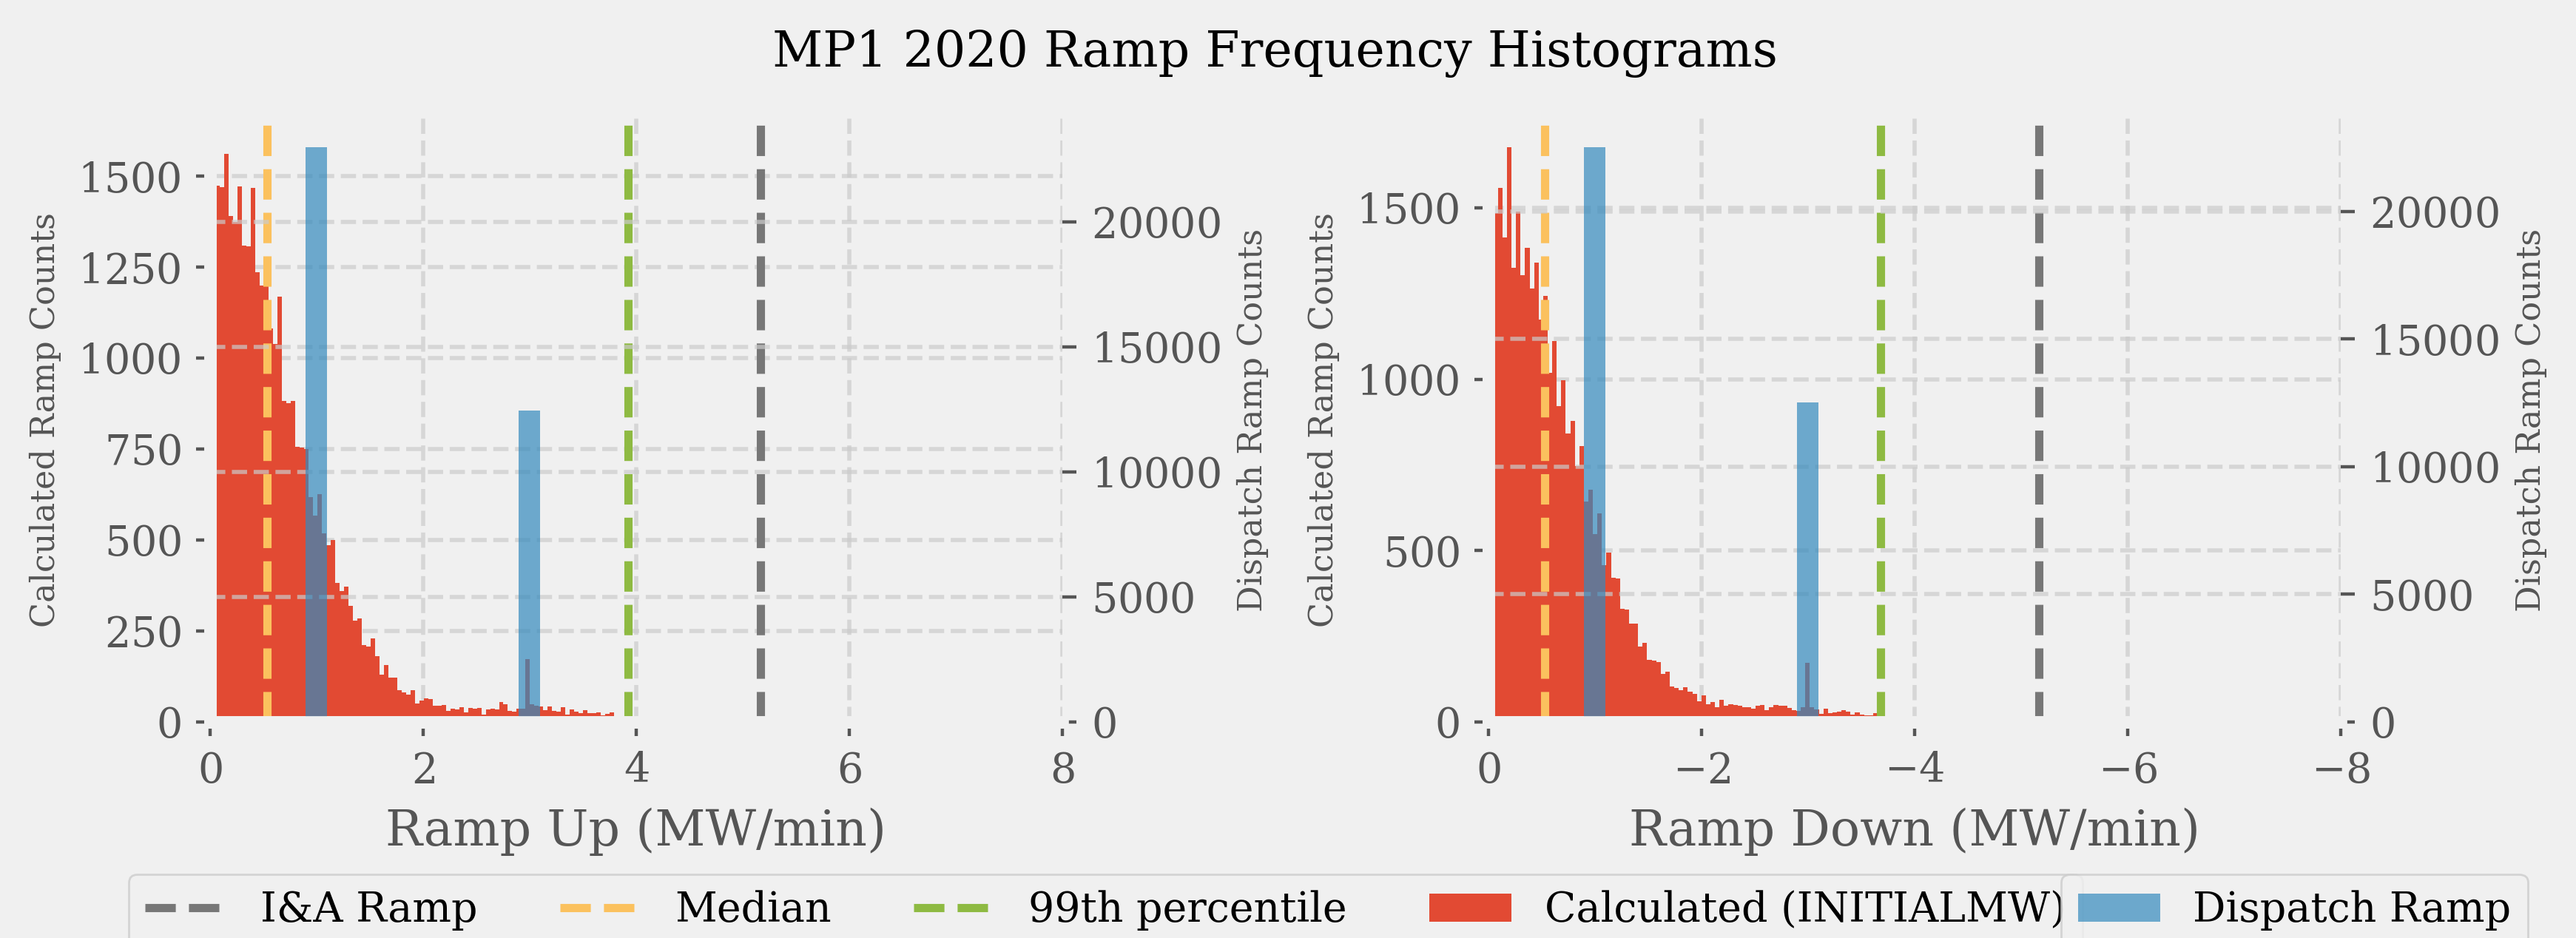
\includegraphics{source/figures/coal_market_upper_ramps.png}
\caption[Observed, submitted and ISP ramp rates for a NSW coal-fired
unit]{Ramp rates observed (red) and used in dispatch by AEMO (blue) for
a coal-fired unit in NSW in 2020. The green line denotes the ramp rate
assumed by AEMO in its 2020 Inputs and Assumptions workbook and the 2020
ISP.}\label{fig:ramp_rate_comparison}
}
\end{figure}

\hypertarget{unit-commitment-and-cycling-constraints}{%
\section{Unit commitment and cycling
constraints}\label{unit-commitment-and-cycling-constraints}}

Many existing flexible conventional resources (OCGT, reciprocating
engines and hydro generation) submit dispatch inflexibility profiles to
AEMO that contain the resource's time to start up and reach MSL, the MSL
itself, the time required at minimum loading and the time taken to shut
down
(\protect\hyperlink{ref-australianenergymarketoperatorFastStartInflexibilityProfile2021}{Australian
Energy Market Operator, 2021s}). The most frequently offered fast start
inflexibility profile of a resource in 2020 was obtained using NEMOSIS
(\protect\hyperlink{ref-gormanNEMOSISNEMOpen2018}{Gorman et al., 2018})
and used to calculate its start-up rate, minimum up-time, MSL and
shutdown rate. The minimum down-time for these resources was chosen to
be equal to the minimum up-time.

For the other conventional resources (CCGT, coal-fired generation and
Gas-Steam), minimum up-times, minimum down-times and MSLs were obtained
from AEMO's 2020 Inputs and Assumptions workbook
(\protect\hyperlink{ref-australianenergymarketoperator2020InputsAssumptions2020}{Australian
Energy Market Operator, 2020p}) and start-up rates were calculated based
on hot or warm start times (i.e.~depending on the start state of the
resource after being offline for its minimum down-time) obtained from
GHD (\protect\hyperlink{ref-ghd2018AEMOCost2018}{2018}) or Aurecon
Australasia
(\protect\hyperlink{ref-aureconaustralasiaGeneratorTechnicalCost2020}{2020}).
The shut-down rates for these resources were calculated based on actual
shutdowns, or those of similar technology types, observed in AEMO
dispatch data that was obtained using NEMOSIS
(\protect\hyperlink{ref-gormanNEMOSISNEMOpen2018}{Gorman et al., 2018}).

BESS were dispatched by PLEXOS's arbitrage algorithm subject to charging
and discharging efficiencies and maximum and minimum state of charge
constraints that corresponded to those assumed within AEMO's 2020 Inputs
and Assumptions workbook
(\protect\hyperlink{ref-australianenergymarketoperator2020InputsAssumptions2020}{Australian
Energy Market Operator, 2020p}). Given an assumed economic lifetime of
10 years
(\protect\hyperlink{ref-australianenergymarketoperator2020InputsAssumptions2020}{Australian
Energy Market Operator, 2020p}) and 3000 cycles
(\protect\hyperlink{ref-dasilvalimaLifeCycleAssessment2021}{da Silva
Lima et al., 2021}) for lithium-ion BESS, a constraint of 300 cycles per
year was applied to BESS in each scenario.

\hypertarget{partial-and-forced-outages}{%
\section{Partial and forced outages}\label{partial-and-forced-outages}}

Maintenance rates, forced outage rates (partial and full) and the
corresponding mean time taken to repair were modelled for all
conventional generation and were sourced from AEMO's 2020 Inputs and
Assumptions workbook
(\protect\hyperlink{ref-australianenergymarketoperator2020InputsAssumptions2020}{Australian
Energy Market Operator, 2020p}).

\hypertarget{sa-synchronous-generation-requirement}{%
\section{SA synchronous generation
requirement}\label{sa-synchronous-generation-requirement}}

At present, certain combinations of synchronous generators are required
to remain online for power system security in SA. Should ahead processes
indicate that the synchronous generation expected to be online and
dispatched is inadequate to provide sufficient system strength in SA,
AEMO will intervene in the market and direct additional synchronous
generation online (\protect\hyperlink{ref-guReviewSystemStrength2019}{Gu
et al., 2019}). The various sufficient combinations of synchronous
generation in SA are outlined in Australian Energy Market Operator
(\protect\hyperlink{ref-australianenergymarketoperatorTransferLimitAdvice2022}{2022g}),
with a decrease in requirements/increase in the allowable asynchronous
generation level following the installation of 4 synchronous condensers
(completed in 2021). To model these requirements, a must-run condition
was imposed on 3 CCGT units and 1 Gas-Steam unit in 2020, and on 2 CCGT
units and 1 Gas-Steam unit in the 2025 scenarios. These combinations
reflect a subset of the sufficient combinations outlined in Australian
Energy Market Operator
(\protect\hyperlink{ref-australianenergymarketoperatorTransferLimitAdvice2022}{2022g}).

\hypertarget{hydro-generation-monthly-energy-constraints}{%
\section{Hydro generation monthly energy
constraints}\label{hydro-generation-monthly-energy-constraints}}

Run-of-river hydro generation and pumped hydro storage in NSW were
aggregated and modelled as dispatchable generation with monthly energy
constraints. These monthly energy constraints correspond to the average
monthly inflows for the Snowy scheme (NSW and Australia's largest hydro
scheme) across financial years 2011 to 2018 (obtained from Australian
Energy Market Operator
(\protect\hyperlink{ref-australianenergymarketoperator2020InputsAssumptions2020}{2020p})).
Though this model for hydro does not account for the additional
generation that could be extracted from pumped storage, the application
of monthly energy constraints could be interpreted as modelling one
pattern of run-of-river hydro operation and/or enforcing the same
reservoir level at the start and end of each month (and thus at the
start and end of each year). Explicitly modelling reservoir schemes,
inflows for individual hydro generators and pumping opportunities for
pumped hydro storage are likely to improve the accuracy of the
methodology proposed in this work for systems with significant shares of
hydropower capacity.

\hypertarget{demand-and-vre-traces}{%
\section{Demand and VRE traces}\label{demand-and-vre-traces}}

Chronological demand traces at 5-minute resolution were used in the
market simulation. For each region, historical operational demand for
2020 at 5-minute resolution was obtained using NEMOSIS
(\protect\hyperlink{ref-gormanNEMOSISNEMOpen2018}{Gorman et al., 2018})
and used as the demand trace for the 2020 scenario. AEMO ISP demand
traces were available for each 2025 scenario at half-hourly resolution
(\protect\hyperlink{ref-australianenergymarketoperator2020DraftISP2019a}{Australian
Energy Market Operator, 2019f}); 5-minute resolution demand traces for
each 2025 scenario were produced by scaling 5-minute historical
operational demand by a corresponding half-hourly scaling factor, which
was calculated as the ratio of the ISP scenario's 2025 demand trace to
the ISP scenario's 2020 demand trace.

Half-hourly chronological solar PV and wind capacity factor traces were
obtained from AEMO's ISP database for each 2020 scenario
(\protect\hyperlink{ref-australianenergymarketoperator2020DraftISP2019}{Australian
Energy Market Operator, 2019g}) and for each 2025 scenario
(\protect\hyperlink{ref-australianenergymarketoperator2020ISPSolar2020}{Australian
Energy Market Operator, 2020s}). Generation traces were obtained by
multiplying the capacity factor trace of a resource by its nameplate
capacity. Capacities for existing and committed VRE plants were obtained
from AEMO's 2020 Inputs and Assumptions workbook
(\protect\hyperlink{ref-australianenergymarketoperator2020InputsAssumptions2020}{Australian
Energy Market Operator, 2020p}) and any additional VRE capacity that was
built out in the 2025 scenarios was assigned to AEMO-designated
Renewable Energy Zones (for which capacity factor traces are available)
based on the ISP's generation capacity outlook. The half-hourly
generation traces for each resource and Renewable Energy Zone in a
region were than aggregated and linearly interpolated for use in the
5-minute resolution market simulation.

\hypertarget{resource-market-offers}{%
\section{Resource market offers}\label{resource-market-offers}}

For all scenarios for a given region, one set of four static
price-quantity pairs were used to represent each resource's offer in the
market simulation. Except for hydro generation, offers were priced
\emph{a priori}. The type of the resource determined how each band was
priced (price bands for each resource type are outlined in
Table~\ref{tbl:resourceoffers}) \footnote{For all conventional
  resources, the distribution of offer prices resembles ``hockey-stick''
  offer curves that are common in the NEM
  (\protect\hyperlink{ref-energysynapseDemandResponseNational2020}{Energy
  Synapse, 2020}) and in other electricity markets
  (\protect\hyperlink{ref-hurlbutProtectingMarketHockey2004}{Hurlbut et
  al., 2004}). Moreover, for most peaking conventional resources, energy
  is offered at or just above the strike price of cap options/futures
  (300 AUD/MWh).}:

\begin{itemize}
\tightlist
\item
  For wind and solar PV generators, the entire available forecasted
  energy was offered at the market floor price to ensure preferential
  dispatch of VRE where possible.
\item
  For baseload conventional resources (coal-fired generation and
  Gas-Steam), the first band was priced at or close to the market floor
  price to ensure the resource's MSL would clear the market. The second
  band was priced close to the short-run marginal cost (SRMC) of the
  resource. The SRMC was calculated using the average heat rate, fuel
  price and variable operating and maintenance cost of each resource
  type obtained from Australian Energy Market Operator
  (\protect\hyperlink{ref-australianenergymarketoperator2020InputsAssumptions2020}{2020p}).
  The third band was priced at a premium relative to the resource's SRMC
  and the fourth band was offered at the market cap price.
\item
  For peaking generation (OCGT and reciprocating engines), the first
  band was priced close to the SRMC of each resource, which was
  calculated in the same manner as for baseload conventional resources.
  The second and third band were offered at a moderate and higher
  premium relative to the resource's SRMC, respectively. The fourth band
  was offered at the market cap price.
\item
  Hydro generation offers were adjusted iteratively to align the
  proportions of annual generation and average market prices of the NSW
  2020 scenario with those calculated from historical data.
\end{itemize}

\def\pandoctableshortcapt{Offers by resource type for NSW and SA across
all scenarios}

\hypertarget{tbl:resourceoffers}{}
\begin{longtable}[]{@{}
  >{\centering\arraybackslash}m{(\columnwidth - 8\tabcolsep) * \real{0.1864}}
  >{\centering\arraybackslash}m{(\columnwidth - 8\tabcolsep) * \real{0.2034}}
  >{\centering\arraybackslash}m{(\columnwidth - 8\tabcolsep) * \real{0.2034}}
  >{\centering\arraybackslash}m{(\columnwidth - 8\tabcolsep) * \real{0.2034}}
  >{\centering\arraybackslash}m{(\columnwidth - 8\tabcolsep) * \real{0.2034}}@{}}
\caption[Offers by resource type for NSW and SA across all
scenarios]{\label{tbl:resourceoffers}Offers by resources type for NSW
and SA across all scenarios. The market floor and cap prices used were
-1000 AUD/MW/hr and 15,000 AUD/MW/hr, respectively.}\tabularnewline
\toprule\noalign{}
\begin{minipage}[b]{\linewidth}\centering
Generator Type
\end{minipage} & \begin{minipage}[b]{\linewidth}\centering
Price Band 1 (AUD/MWh)
\end{minipage} & \begin{minipage}[b]{\linewidth}\centering
Price Band 2 (AUD/MWh)
\end{minipage} & \begin{minipage}[b]{\linewidth}\centering
Price Band 3 (AUD/MWh)
\end{minipage} & \begin{minipage}[b]{\linewidth}\centering
Price Band 4 (AUD/MWh)
\end{minipage} \\
\midrule\noalign{}
\endfirsthead
\toprule\noalign{}
\begin{minipage}[b]{\linewidth}\centering
Generator Type
\end{minipage} & \begin{minipage}[b]{\linewidth}\centering
Price Band 1 (AUD/MWh)
\end{minipage} & \begin{minipage}[b]{\linewidth}\centering
Price Band 2 (AUD/MWh)
\end{minipage} & \begin{minipage}[b]{\linewidth}\centering
Price Band 3 (AUD/MWh)
\end{minipage} & \begin{minipage}[b]{\linewidth}\centering
Price Band 4 (AUD/MWh)
\end{minipage} \\
\midrule\noalign{}
\endhead
\bottomrule\noalign{}
\endlastfoot
Coal & Floor & 30 & 50 & Cap \\
CCGT & 40/Floor (NSW/SA) & 70 & 170 & - \\
OCGT & 100/175 (NSW/SA) & 200/300 (NSW/SA) & 500 & Cap \\
Reciprocating Engine & 175 & 300 & 500 & Cap \\
Gas-Steam & Floor & 90 & 190 & Cap \\
Wind & Floor & - & - & - \\
Solar PV & Floor & - & - & - \\
Hydro & 35 & 60 & 300 & Cap \\
\end{longtable}

\let\pandoctableshortcapt\relax

\hypertarget{sec:calibration}{%
\subsection*{Calibration}\label{sec:calibration}}
\addcontentsline{toc}{subsection}{Calibration}

Resource offer quantities were used to calibrate the 2020 simulation
with historical generation patterns in each state. The quantity of
energy in each price band was adjusted in an iterative process of offer
adjustment and market simulation to ensure that the proportion of annual
generation of a particular resource type in the simulated 2020 scenario
was similar to the actual proportion of annual generation for that
resource type in 2020. The combination of offer quantities that produced
the closest proportions were retained and used for each state's 2020 and
2025 scenarios. The results of the calibration for NSW and SA are
outlined in Table~\ref{tbl:nswcalibration} and
Table~\ref{tbl:sacalibration}, respectively.

\def\pandoctableshortcapt{NSW 2020 calibration results (by resource
type)}

\hypertarget{tbl:nswcalibration}{}
\begin{longtable}[]{@{}lcccccc@{}}
\caption[NSW 2020 calibration results (by resource
type)]{\label{tbl:nswcalibration}Percentage of annual generation by
resource type for the simulated NSW 2020 scenario and for NSW in 2020
(calculated based on historical data obtained using NEMOSIS
(\protect\hyperlink{ref-gormanNEMOSISNEMOpen2018}{Gorman et al.,
2018})).}\tabularnewline
\toprule\noalign{}
& Coal & Wind & Hydro & Solar PV & CCGT & OCGT \\
\midrule\noalign{}
\endfirsthead
\toprule\noalign{}
& Coal & Wind & Hydro & Solar PV & CCGT & OCGT \\
\midrule\noalign{}
\endhead
\bottomrule\noalign{}
\endlastfoot
NSW 2020 & 82.9\% & 6.4\% & 4.5\% & 3.2\% & 2.4\% & 0.6\% \\
Historical 2020 & 84.5\% & 6.6\% & 3.8\% & 3.3\% & 1.5\% & 0.3\% \\
\end{longtable}

\let\pandoctableshortcapt\relax

\def\pandoctableshortcapt{SA 2020 calibration results (by resource
type)}

\hypertarget{tbl:sacalibration}{}
\begin{longtable}[]{@{}
  >{\raggedright\arraybackslash}m{(\columnwidth - 12\tabcolsep) * \real{0.2125}}
  >{\centering\arraybackslash}m{(\columnwidth - 12\tabcolsep) * \real{0.0875}}
  >{\centering\arraybackslash}m{(\columnwidth - 12\tabcolsep) * \real{0.0875}}
  >{\centering\arraybackslash}m{(\columnwidth - 12\tabcolsep) * \real{0.1375}}
  >{\centering\arraybackslash}m{(\columnwidth - 12\tabcolsep) * \real{0.1250}}
  >{\centering\arraybackslash}m{(\columnwidth - 12\tabcolsep) * \real{0.0750}}
  >{\centering\arraybackslash}m{(\columnwidth - 12\tabcolsep) * \real{0.2750}}@{}}
\caption[SA 2020 calibration results (by resource
type)]{\label{tbl:sacalibration}Percentage of annual generation by
resource type for the simulated SA 2020 scenario and for SA in 2020
(calculated based on historical data obtained using NEMOSIS
(\protect\hyperlink{ref-gormanNEMOSISNEMOpen2018}{Gorman et al.,
2018})). Note that percentages may not sum to a total of 100\% due to
net storage in BESS.}\tabularnewline
\toprule\noalign{}
\begin{minipage}[b]{\linewidth}\raggedright
\end{minipage} & \begin{minipage}[b]{\linewidth}\centering
Wind
\end{minipage} & \begin{minipage}[b]{\linewidth}\centering
CCGT
\end{minipage} & \begin{minipage}[b]{\linewidth}\centering
Gas-Steam
\end{minipage} & \begin{minipage}[b]{\linewidth}\centering
Solar PV
\end{minipage} & \begin{minipage}[b]{\linewidth}\centering
OCGT
\end{minipage} & \begin{minipage}[b]{\linewidth}\centering
Reciprocating Engine
\end{minipage} \\
\midrule\noalign{}
\endfirsthead
\toprule\noalign{}
\begin{minipage}[b]{\linewidth}\raggedright
\end{minipage} & \begin{minipage}[b]{\linewidth}\centering
Wind
\end{minipage} & \begin{minipage}[b]{\linewidth}\centering
CCGT
\end{minipage} & \begin{minipage}[b]{\linewidth}\centering
Gas-Steam
\end{minipage} & \begin{minipage}[b]{\linewidth}\centering
Solar PV
\end{minipage} & \begin{minipage}[b]{\linewidth}\centering
OCGT
\end{minipage} & \begin{minipage}[b]{\linewidth}\centering
Reciprocating Engine
\end{minipage} \\
\midrule\noalign{}
\endhead
\bottomrule\noalign{}
\endlastfoot
Historical 2020 & 43.7\% & 29.7\% & 15.1\% & 5.1\% & 2.3\% & 3.5\% \\
SA 2020 & 45.6\% & 25.6\% & 16.8\% & 8.0\% & 2.3\% & 1.6\% \\
\end{longtable}

\let\pandoctableshortcapt\relax

\hypertarget{sec:appendix-milps}{%
\chapter{Mixed integer linear program
formulations}\label{sec:appendix-milps}}

\hypertarget{sec:appendix-milps-assumptions}{%
\section{Assumed battery energy storage system operating
characteristics}\label{sec:appendix-milps-assumptions}}

We model a lithium-ion BESS and assume the following with respect to its
operating characteristics:

\begin{itemize}
\tightlist
\item
  The BESS is highly flexible; it has no minimum operating levels and
  can ramp between charging at its maximum power output in one dispatch
  interval to discharging at its maximum power output in the next (or
  vice versa).
\item
  The BESS is only cycled between lower and upper state-of-charge limits
  (fixed at 10\% and 90\%, respectively). Such limits are often imposed
  by storage operators to avoid the accelerated degradation that
  accompanies deep discharging (particularly for
  lithium-nickel-manganese-cobalt-oxide batteries)
  (\protect\hyperlink{ref-xuRoleModelingBattery2022}{Xu, 2022}), and to
  ensure that market participation obligations can be met by the storage
  device. Given these state-of-charge constraints and assuming that the
  BESS is operated at its nominal temperature, current and voltage, we
  assume that its charging and discharging efficiencies remain constant
  and fix both at 91\% (including inverter losses)
  (\protect\hyperlink{ref-daviesCombinedEconomicTechnological2019}{Davies
  et al., 2019};
  \protect\hyperlink{ref-yangModellingOptimalEnergy2022}{Yang et al.,
  2022}). Combined, these efficiencies yield an ESR round-trip
  efficiency of \textasciitilde83\%, which is consistent with values
  used in similar studies
  (\protect\hyperlink{ref-mcphersonImpactsStorageDispatch2020}{McPherson
  et al., 2020}; \protect\hyperlink{ref-xuRoleModelingBattery2022}{Xu,
  2022};
  \protect\hyperlink{ref-yurdakulRiskAverseSelfSchedulingStorage2023}{Ogun
  Yurdakul and Billimoria, 2023}).
\item
  Self-discharge losses are negligible for a lithium-ion BESS
  (\protect\hyperlink{ref-bradburyEconomicViabilityEnergy2014}{Bradbury
  et al., 2014}).
\item
  Given that we only model one year of operation, we ignore BESS
  capacity fade due to cycle and calendar degradation. The latter
  constitutes an additional opportunity-cost that may modify the
  attractiveness of certain arbitrage opportunities, particularly if
  operation over the entire lifetime of the BESS is modelled
  (\protect\hyperlink{ref-wattsEffectsBatteryDegradation2022}{Watts and
  MacGill, 2022}; \protect\hyperlink{ref-xuRoleModelingBattery2022}{Xu,
  2022}).
\end{itemize}

\hypertarget{nomenclature}{%
\section{Nomenclature}\label{nomenclature}}

\hypertarget{indices-and-sets-1}{%
\subsection{Indices and sets}\label{indices-and-sets-1}}

\begin{description}[leftmargin=8em,style=nextline]
  \item[$\mathcal{T}$] Ordered set of time periods within the lookahead horizon, i.e. $\mathcal{T} = \{1, 2, 3, ..., T\}$
  \item[$t \in \mathcal{T}$] Time period $t$ in the lookahead horizon. In this study, each $t$ corresponds to the end of a 5-minute dispatch interval
\end{description}

\hypertarget{parameters}{%
\subsection{Parameters}\label{parameters}}

\begin{description}[leftmargin=8em,style=nextline]
  \item[$\tau$] Time duration of a dispatch interval (5 minutes or $\frac{1}{12}$ hours)
  \item[$\lambda_t$] Energy price (forecast or actual) at time $t$ (AUD/MW/hr)
  \item[$\bar{p}$] Maximum power capacity of BESS (MW)
  \item[$\underline{e}$] Minimum level of energy storage (MWh). Fixed at 10\% of energy capacity for all models
  \item[$\bar{e}$] Maximum level of energy storage (MWh). Fixed at 90\% of energy capacity for all models
  \item[$\eta_{\textrm{charge}}$] Charging efficiency (unitless). Fixed at 91\% for all models
  \item[$\eta_{\textrm{discharge}}$] Discharging efficiency (unitless). Fixed at 91\% for all models
  \item[$e_0$] Initial level of energy storage. Fixed at 50\% of energy capacity for the first scheduling step and, for successive steps, is calculated using the binding decision of the last step
  \item[$d_0$] Initial energy storage throughput (MWh). Fixed at 0 MWh for the first scheduling step and, for successive steps, is calculated using the binding decision of the last step
  \item[$d_{\textrm{lifetime}}$] Cumulative energy throughput lifetime of the BESS (MWh). See Table 1 for the values assumed in calculating this parameter.
  \item[$e_{\textrm{rated}}$] Rated (i.e. initial) energy storage capacity of the BESS (MWh). Fixed at 100 MWh for all BESS in this study.
  \item[$c_{\textrm{capital}}$] BESS capital cost per unit of energy storage (AUD/MWh). See Table 1 for the range of capital costs tested in this study.
\end{description}

\hypertarget{variables}{%
\subsection{Variables}\label{variables}}

\begin{description}[leftmargin=8em,style=nextline]
  \item[$u_t$] Charge state binary variable, i.e. value of 1 if BESS is charging at time $t$ (unitless)
  \item[$e_t$] Level of energy storage at time $t$ (MWh)
  \item[$p_t$] Discharging power of BESS at time $t$ (MW)
  \item[$q_t$] Charging power of BESS at time $t$ (MW)
  \item[$d_t$] Cumulative BESS energy throughput at time $t$ (MWh)
\end{description}

\hypertarget{sec:appendix-milps-arb}{%
\section{Arbitrage}\label{sec:appendix-milps-arb}}

\begin{maxi!}[2]
    {p_t,q_t}{\sum_{t \in \mathcal{T}}{\tau\lambda_t(p_t-q_t)} \label{eq:arb-1a}}
    {}{}
    \addConstraint{u_t}{\in \{0,1\} \label{eq:arb-1b}}  
    \addConstraint{p_t}{\geq 0 \label{eq:arb-1c}}
    \addConstraint{q_t}{\geq 0 \label{eq:arb-1d}}
    \addConstraint{p_t - \bar{p}\left(1-u_t\right)}{\leq 0 \label{eq:arb-1e}}
    \addConstraint{q_t - \bar{p}u_t}{\leq 0 \label{eq:arb-1f}}
    \addConstraint{\underline{e} \leq e_t \leq \bar{e}}{\label{eq:arb-1g}}
    \addConstraint{e_t-e_{t-1}- \left( q_t\eta_{\textrm{charge}}\tau\right)+\frac{p_t\tau}{\eta_{\textrm{discharge}}}}{= 0 \label{eq:arb-1h}}
    \addConstraint{e_1 - e_0 - \left( q_1\eta_{\textrm{charge}}\tau\right)+\frac{p_1\tau}{\eta_{\textrm{discharge}}}}{= 0 \label{eq:arb-1i}}
\end{maxi!}

Equation~\ref{eq:arb-1a} maximises arbitrage revenue over the scheduling
lookahead horizon. Equation~\ref{eq:arb-1c} and Equation~\ref{eq:arb-1d}
ensure that discharging and charging, respectively, are greater than or
equal to 0 MW, and Equation~\ref{eq:arb-1b} introduces binary charge
state variables that are used in Equation~\ref{eq:arb-1e} and
Equation~\ref{eq:arb-1f} to enforce the BESS maximum power capacity
limit and prevent the BESS from simultaneously discharging and charging
in the same dispatch interval. Equation~\ref{eq:arb-1g} enforces BESS
energy storage limits (the rationale for which we previously discussed
in Section~\ref{sec:appendix-milps-assumptions}), and
Equation~\ref{eq:arb-1h} and Equation~\ref{eq:arb-1i} are intertemporal
constraints that model BESS state-of-charge evolution.

\hypertarget{sec:appendix-milps-arbpen}{%
\section{Arbitrage with throughput
penalty}\label{sec:appendix-milps-arbpen}}

\begin{maxi!}[2]
    {p_t,q_t}{\sum_{t \in \mathcal{T}}{\tau\lambda_t(p_t-q_t)}  - \frac{d_T - d_0}{d_{\textrm{lifetime}}} e_{\textrm{rated}} c_{\textrm{capital}} \label{eq:arb-2a}}
    {}{}
    \addConstraint{u_t}{\in \{0,1\}} 
    \addConstraint{p_t}{\geq 0}
    \addConstraint{q_t}{\geq 0}
    \addConstraint{p_t - \bar{p}\left(1-u_t\right)}{\leq 0}
    \addConstraint{q_t - \bar{p}u_t}{\leq 0}
    \addConstraint{\underline{e} \leq e_t \leq \bar{e}}{}
    \addConstraint{e_t-e_{t-1}- \left( q_t\eta_{\textrm{charge}}\tau\right)+\frac{p_t\tau}{\eta_{\textrm{discharge}}}}{= 0}
    \addConstraint{e_1 - e_0 - \left( q_1\eta_{\textrm{charge}}\tau\right)+\frac{p_1\tau}{\eta_{\textrm{discharge}}}}{= 0}
    \addConstraint{e_t-e_{t-1}- \left( q_t\eta_{\textrm{charge}}\tau\right)+\frac{p_t\tau}{\eta_{\textrm{discharge}}}}{= 0}
    \addConstraint{d_t-d_{t-1} - p_t\tau}{= 0 \label{eq:arb-2j}}
    \addConstraint{d_1-d_0 - p_1\tau}{= 0 \label{eq:arb-2k}}
\end{maxi!}

Equation~\ref{eq:arb-2a} maximises arbitrage revenue over the scheduling
lookahead horizon given a penalty on the throughput accrued by the BESS
over the optimisation window. The penalty corresponds to the additional
BESS throughput accrued over the scheduling lookahead horizon
(i.e.~\(d_T - d_0\)) divided by the assumed BESS warrantied throughput
lifetime (\(d_{\textrm{lifetime}}\)) and multiplied by the assumed BESS
capital cost (the product of \(e_{\textrm{rated}}\) and
\(c_{\textrm{capital}}\)) (see Table~\ref{tbl:formulations} for assumed
values). Constraints Equation~\ref{eq:arb-2j} and
Equation~\ref{eq:arb-2k} are intertemporal constraints that model BESS
cumulative throughput evolution. All other constraints are described in
Section~\ref{sec:appendix-milps-arb}.

\hypertarget{sec:appendix-milps-arbdisc}{%
\section{Arbitrage with discounting}\label{sec:appendix-milps-arbdisc}}

\begin{maxi!}[2]
    {p_t,q_t}{\sum_{t \in \mathcal{T}}\left(\tau(p_t - q_t) \times \lambda_t DF(r, t-t_0) \right)  - \frac{d_T - d_0}{d_{\textrm{lifetime}}} e_{\textrm{rated}} c_{\textrm{capital}} \label{eq:arb-3a}}
    {}{}
    \addConstraint{u_t}{\in \{0,1\}}
    \addConstraint{p_t}{\geq 0}
    \addConstraint{q_t}{\geq 0}
    \addConstraint{p_t - \bar{p}\left(1-u_t\right)}{\leq 0}
    \addConstraint{q_t - \bar{p}u_t}{\leq 0}
    \addConstraint{\underline{e} \leq e_t \leq \bar{e}}{}
    \addConstraint{e_t-e_{t-1}- \left( q_t\eta_{\textrm{charge}}\tau\right)+\frac{p_t\tau}{\eta_{\textrm{discharge}}}}{= 0}
    \addConstraint{e_1 - e_0 - \left( q_1\eta_{\textrm{charge}}\tau\right)+\frac{p_1\tau}{\eta_{\textrm{discharge}}}}{= 0}
    \addConstraint{e_t-e_{t-1}- \left( q_t\eta_{\textrm{charge}}\tau\right)+\frac{p_t\tau}{\eta_{\textrm{discharge}}}}{= 0}
    \addConstraint{d_t-d_{t-1} - p_t\tau}{= 0}
    \addConstraint{d_1-d_0 - p_1\tau}{= 0}
\end{maxi!}

Equation~\ref{eq:arb-3a} maximises arbitrage revenue over the scheduling
lookahead horizon given discounted future prices
(i.e.~\(\lambda_t DF(r,t-t_0)\)) and a penalty on the throughput accrued
by the BESS over the optimisation window. The discount function \(DF\)
is either exponential or hyperbolic, and takes a discount rate \(r\) and
forecast ahead time \(t-t_0\) as arguments. Refer to the next appendix
(Section~\ref{sec:appendix-discounting}) for the discount function
formulae, the methodology for determining discount rates and the
discount rate values used in this study's storage modelling. All other
constraints are described in Section~\ref{sec:appendix-milps-arb} and
Section~\ref{sec:appendix-milps-arbpen}.

\hypertarget{sec:appendix-discounting}{%
\chapter{Methodology for discounting future price
forecasts}\label{sec:appendix-discounting}}

Delay discounting was used to model a scheduler's belief that price
forecasts will improve as the forecast run time approaches the
forecasted delivery time. In other words, discounting price forecasts
further into the future represents a time preference for
\emph{information}. The rationale for discounting price forecasts is
that it can provide robustness to ESR operation by reducing the
attractiveness of uncertain opportunities. However it is also
problematic as ``devaluing'' revenues and costs in the near future
(i.e.~up to a day-ahead) is not reflective of the time periods over
which a storage operator's time preferences are stronger (i.e.~over
multiple months and years). Devaluing future revenues and costs could
also lead to missed opportunities (e.g.~due to discounted price spikes)
and poor decisions (e.g.~discounted lower prices that make charging more
attractive than it otherwise would be).

Two discounting functions were tested: an exponential discounting
function (Equation~\ref{eq:exponential-discounting}), which is commonly
used in finance and neoclassical economics, and a hyperbolic discounting
function (Equation~\ref{eq:hyperbolic-discounting}), which has been used
to model empirical evidence of intertemporal inconsistency in
decision-making
(\protect\hyperlink{ref-ainslieSpeciousRewardBehavioral1975}{Ainslie,
1975};
\protect\hyperlink{ref-grune-yanoffModelsTemporalDiscounting2015}{Grüne-Yanoff,
2015}). Instead of using the hyperbolic discount function to model the
\emph{choice} of a decision-maker, we use it to model a potential
\emph{belief} about information they might hold: that price forecasts
further into the future are likely to be more-or-less equally
``untrustworthy'' (e.g.~a forecast made 8 hours ahead might be as
``inaccurate'' as a forecast made 12 hours ahead).

\begin{equation}\protect\hypertarget{eq:exponential-discounting}{}{DF(r, t-t_0) = e^{-r(t-t_0)}}\label{eq:exponential-discounting}\end{equation}

\begin{equation}\protect\hypertarget{eq:hyperbolic-discounting}{}{DF(r, t-t_0) = \frac{1}{1+r(t-t_0)}}\label{eq:hyperbolic-discounting}\end{equation}

Given their importance to market participants, counts of significant
pre-dispatch price forecast errors
(Figure~\ref{fig:nsw_significant_price_error_counts}) were used to
calculate a discount rate for each function (i.e.~\(r\), in units
\(hr^{-1}\)). Significant price forecast error price counts were
max-scaled (i.e.~counts at each ahead time were divided by the counts at
24 hours ahead) and then subtracted from one to produce the red curve in
Figure~\ref{fig:discount_function_fitting}. The exponential and
hyperbolic discount functions were then fitted to this curve using curve
fitting tools in the \texttt{scipy} package
(\protect\hyperlink{ref-mckinney-proc-scipy-2010}{McKinney, 2010}). The
values of \(r\) obtained from this process (outlined in
Table~\ref{tbl:discount-rates}) were then used alongside their
corresponding discount functions in the arbitrage with discounting MILP
formulation (Section~\ref{sec:appendix-milps-arbdisc}).

\def\pandoctableshortcapt{Discount rates and RMSD from each discount
function fit}

\hypertarget{tbl:discount-rates}{}
\begin{longtable}[]{@{}
  >{\raggedright\arraybackslash}m{(\columnwidth - 4\tabcolsep) * \real{0.3291}}
  >{\raggedright\arraybackslash}m{(\columnwidth - 4\tabcolsep) * \real{0.3291}}
  >{\raggedright\arraybackslash}m{(\columnwidth - 4\tabcolsep) * \real{0.3291}}@{}}
\caption[Discount rates and RMSD from each discount function
fit]{\label{tbl:discount-rates}Discount rates obtained from fitting
discount functions to max-scaled significant price forecast error counts
over time, and the root-mean-square deviation (RMSD) of each
fit.}\tabularnewline
\toprule\noalign{}
\endfirsthead
\endhead
\bottomrule\noalign{}
\endlastfoot
& Exponential & Hyperbolic \\
Discount rate (\(hr^{-1}\)) & 0.1994 & 0.4203 \\
RMSD & 0.088 & 0.049 \\
\end{longtable}

\let\pandoctableshortcapt\relax

\begin{figure}
\hypertarget{fig:nsw_significant_price_error_counts}{%
\centering
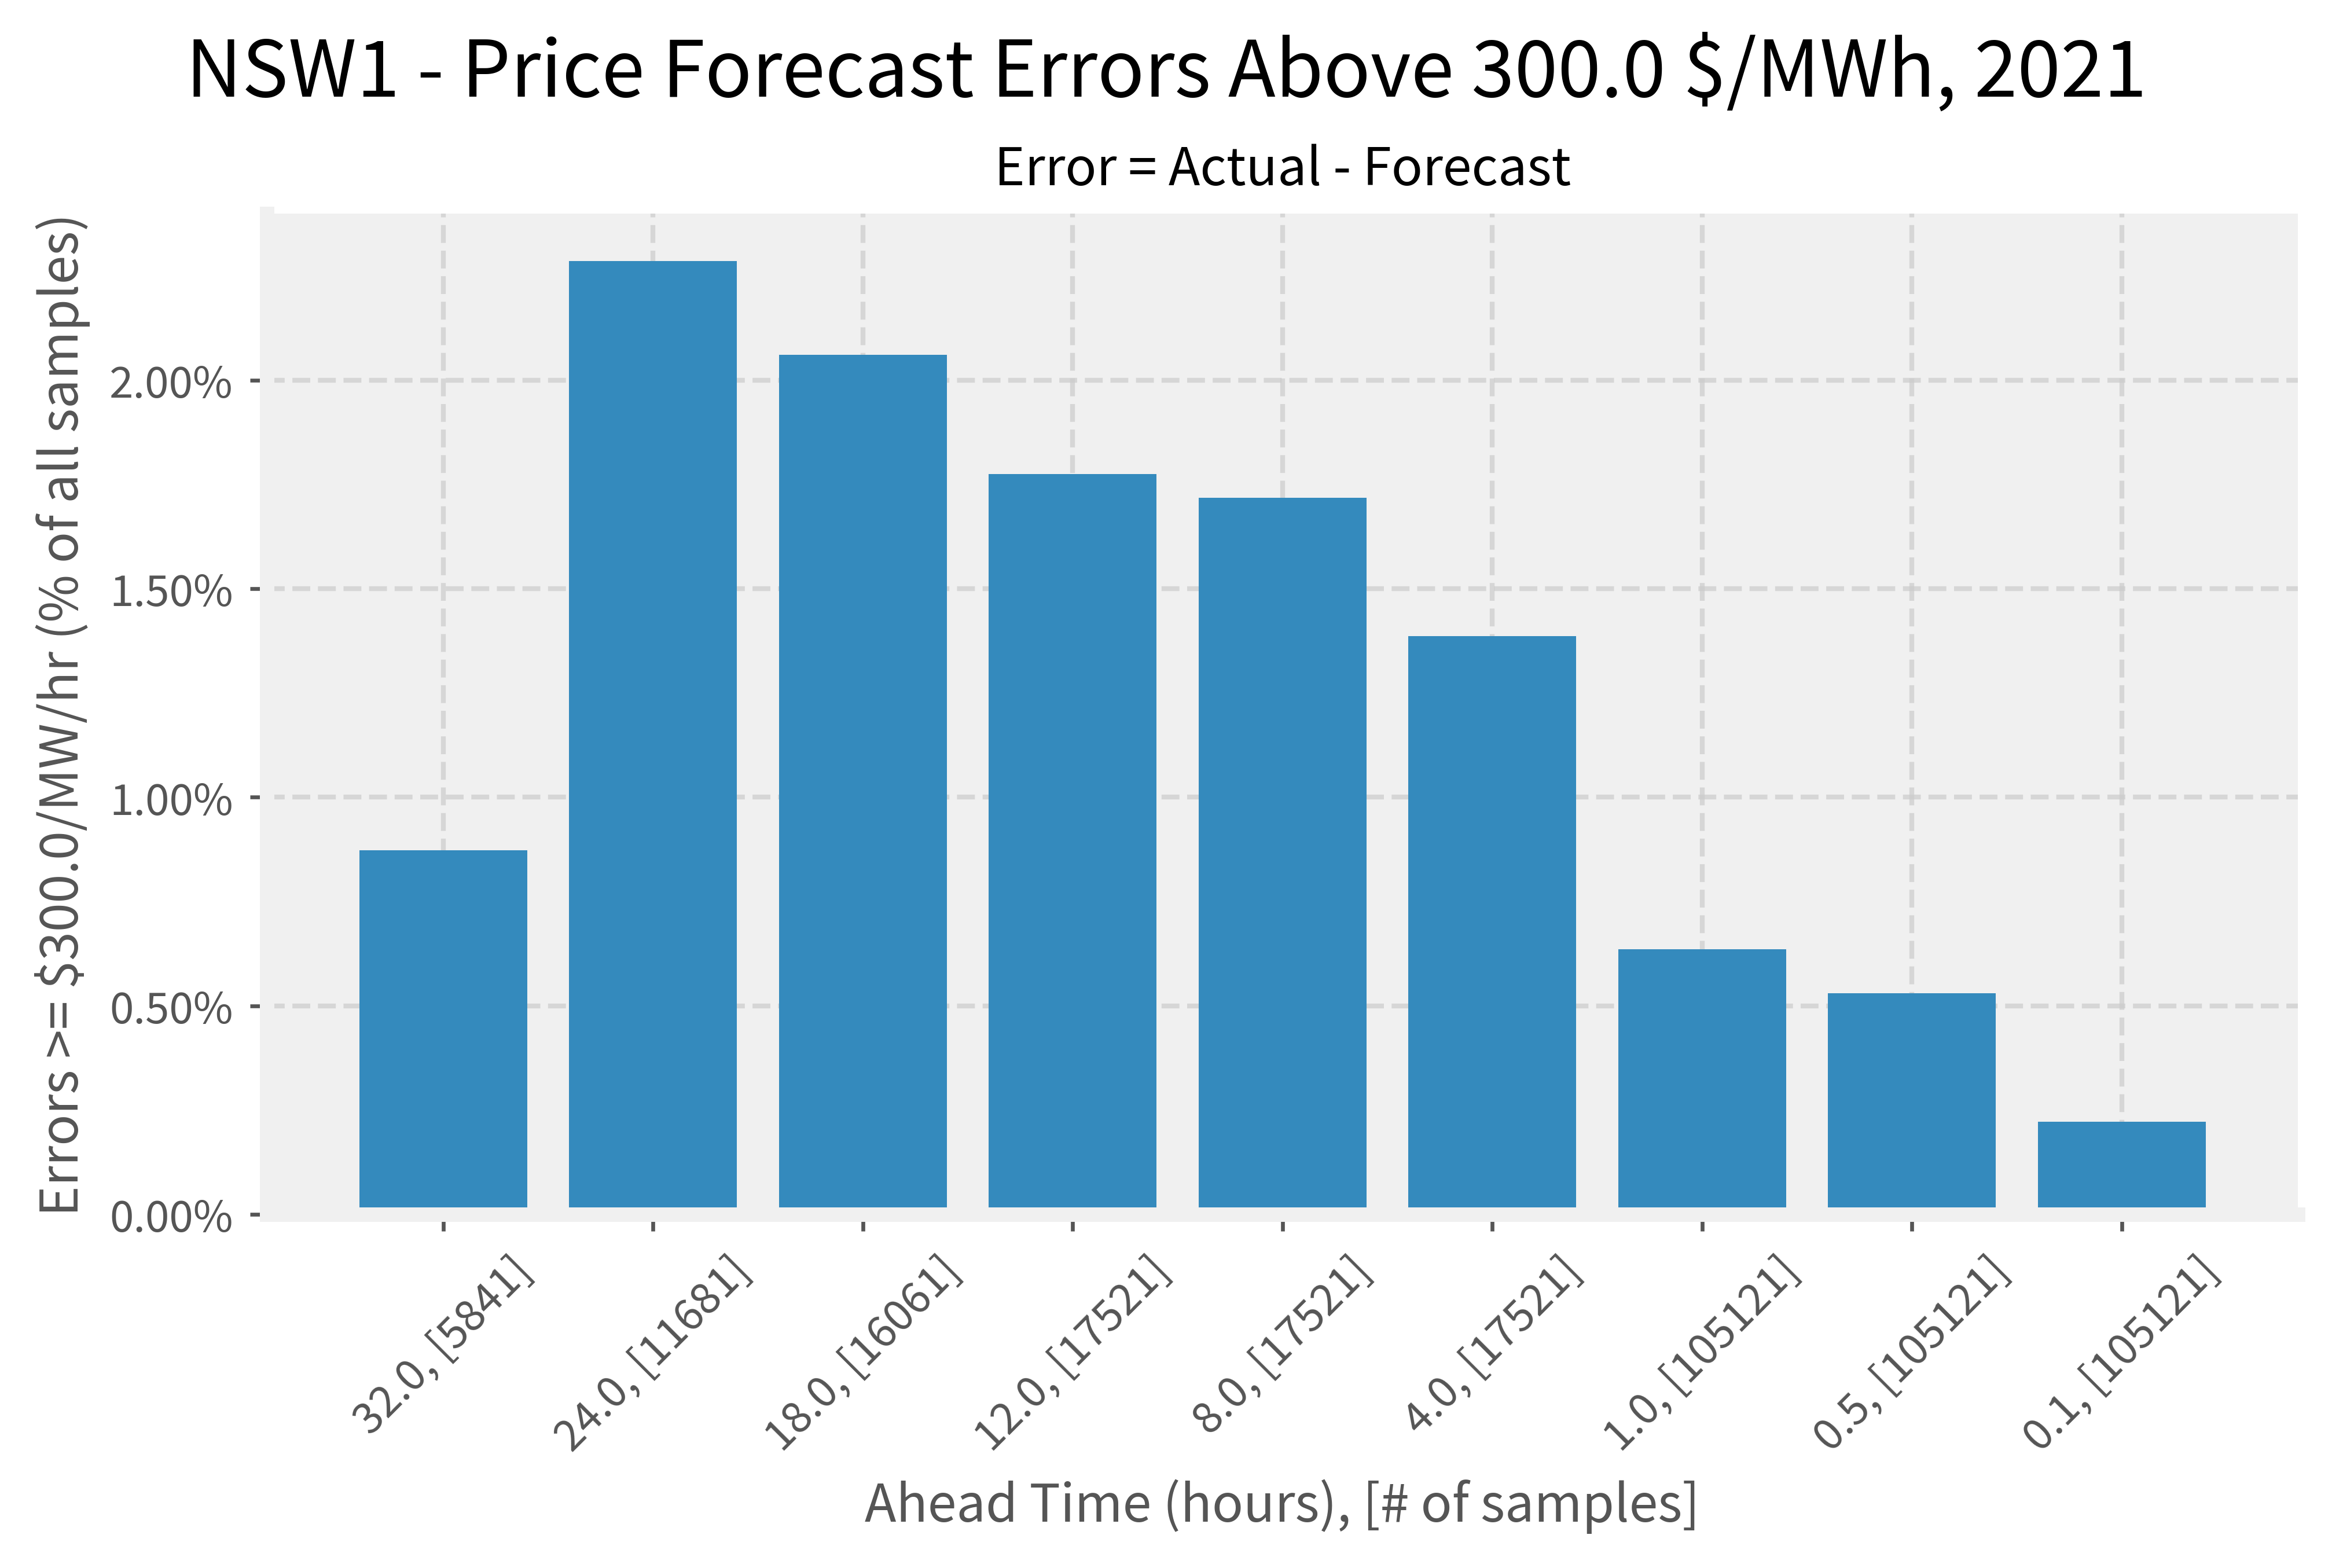
\includegraphics{source/figures/NSW1_percent_above_300.0_2021.png}
\caption[Count of significant price errors by forecast ahead
time]{Significant price forecast errors (i.e.~\textgreater{} 300
AUD/MW/hr, see Section~\ref{sec:info-case_study-price_forecast_errors}
for a definition of ``significant'') as a proportion of all price
forecast errors for a given forecast ahead time in NSW in 2021. The
horizontal axis labels show both the forecast ahead time in hours and
the number of price forecast error samples for that ahead time in square
brackets. The number of samples decreases beyond 16 hours (the reason
for which is outlined in
Section~\ref{sec:info-case_study-bess_simulations-method-price_data})
and increases within an hour of delivery as forecasts within this
horizon are published more frequently (i.e.~5MPD is published every 5
minutes). The decrease in the proportion of significant price forecast
errors from forecasts 24 hours out to forecasts 32 hours out could be
explained by the latter forecasting periods late at night or early in
the morning -- periods when supply and demand conditions are typically
more stable and thus predictable
(\protect\hyperlink{ref-prakashLookingPredispatchDemand2023}{Prakash,
2023c}). Pre-dispatch price forecast data were obtained using
\texttt{NEMSEER}
(\protect\hyperlink{ref-prakashNEMSEERPythonPackage2023}{Prakash et al.,
2023b}), and actual market price data were obtained using
\texttt{NEMOSIS}
(\protect\hyperlink{ref-gormanNEMOSISNEMOpen2018}{Gorman et al., 2018}).
Errors within an hour of delivery were calculated using 5MPD forecasts.
Refer the research data for this article for further details and source
code. This plot was generated using \texttt{matplotlib}
(\protect\hyperlink{ref-hunterMatplotlib2DGraphics2007}{Hunter,
2007}).}\label{fig:nsw_significant_price_error_counts}
}
\end{figure}

Though the hyperbolic discount function obtains a better fit and
reflects the intuition that forecasts say 15 hours out and 20 hours out
are equally questionable, it discounts price forecasts closer to
real-time (\(\lessapprox\) 6 hours) to a greater degree than the
exponential discount function
(Figure~\ref{fig:discount_function_fitting}). As we outline in
Section~\ref{sec:info-case_study-bess_simulations-method-results}, this
may, in some cases, lead to poorer arbitrage performance than if an
exponential discount function were used.

\begin{figure}
\hypertarget{fig:discount_function_fitting}{%
\centering
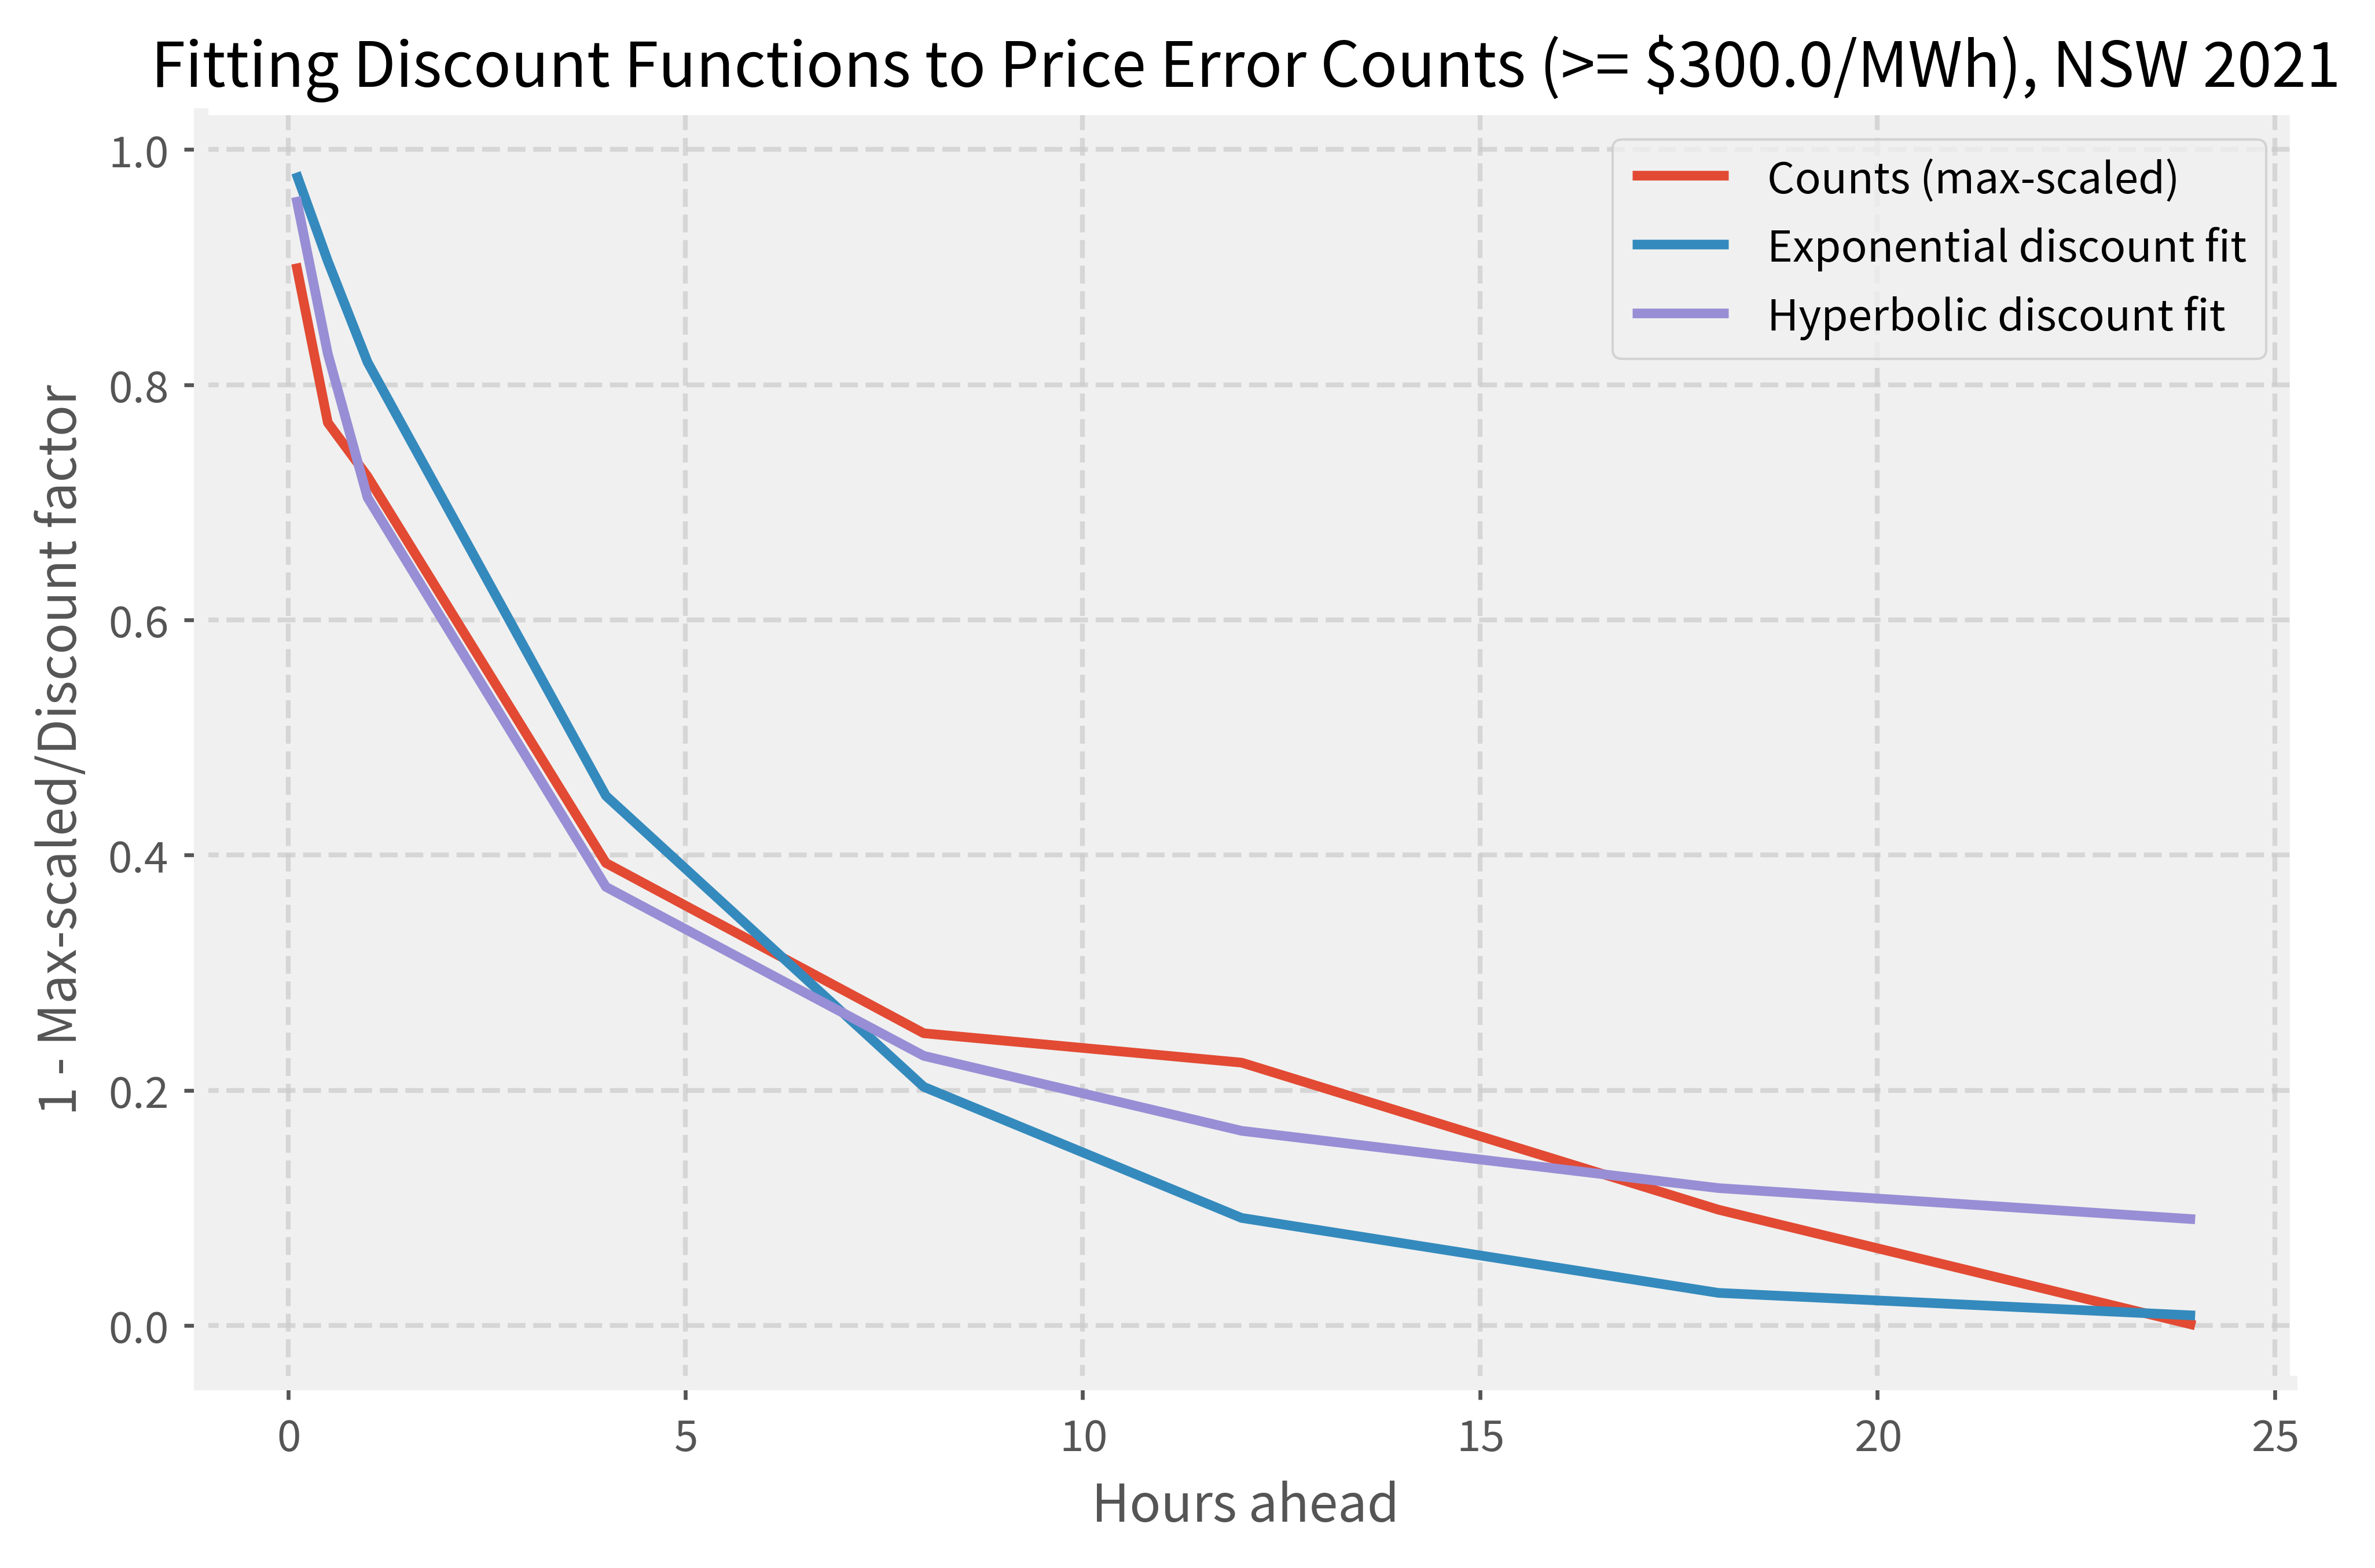
\includegraphics{source/figures/curve_fits_300.0.png}
\caption[Price forecast error counts for NSW in 2021, and the fitted
exponential and hyperbolic discount functions]{Discount function fits to
the price forecast error counts for NSW in 2021. To ensure that
forecasts further out from delivery were discounted to a greater degree,
significant price forecast errors counts were max-scaled and then
subtracted from one
(i.e.~\(1-\frac{\textrm{counts}_{\textrm{ahead time}}}{\textrm{counts}_{\textrm{24 hours ahead}}}\))}\label{fig:discount_function_fitting}
}
\end{figure}

\footnotesize
\singlespacing
\setlength{\parindent}{0in}

\hypertarget{references}{%
\chapter*{References}\label{references}}
\addcontentsline{toc}{chapter}{References}

\hypertarget{refs}{}
\begin{CSLReferences}{1}{0}
\leavevmode\vadjust pre{\hypertarget{ref-50hzamprionapgeliartetennetConsultationDesignPlatform2017}{}}%
50hz, A., Amprion, 2017. Consultation on the design of the platform for
automatic {Frequency Restoration Reserve} ({aFRR}) of {PICASSO} region.

\leavevmode\vadjust pre{\hypertarget{ref-abbasyNationalDesignMultinational2012}{}}%
Abbasy, A., 2012.
\href{https://doi.org/10.4233/uuid:71f7138f-3af2-4bc3-b035-a3e42b3cafaf}{National
{Design} and {Multinational Integration} of {Balancing Services
Markets}}. {TU Delft}.

\leavevmode\vadjust pre{\hypertarget{ref-abdullaOptimalOperationEnergy2018}{}}%
Abdulla, K., de Hoog, J., Muenzel, V., Suits, F., Steer, K., Wirth, A.,
Halgamuge, S., 2018. Optimal {Operation} of {Energy Storage Systems
Considering Forecasts} and {Battery Degradation}. IEEE Transactions on
Smart Grid 9, 2086--2096. \url{https://doi.org/10.1109/TSG.2016.2606490}

\leavevmode\vadjust pre{\hypertarget{ref-achillesIntegratingInverterBasedResources2017}{}}%
Achilles, S., Isaacs, A., MacDowell, J., Conto, J., Hsu, S.-M., Hindi,
H., McBride, A., Osman, M., Quint, R., 2017. Integrating {Inverter-Based
Resources} into {Low Short Circuit Strength Systems}.

\leavevmode\vadjust pre{\hypertarget{ref-agoraenergiewendeFlexibilityThermalPower2017}{}}%
Agora Energiewende, 2017. Flexibility in thermal power plants {With} a
focus on existing coal-fired power plants.

\leavevmode\vadjust pre{\hypertarget{ref-ahlqvistSurveyComparingCentralized2022}{}}%
Ahlqvist, V., Holmberg, P., Tangerås, T., 2022. A survey comparing
centralized and decentralized electricity markets. Energy Strategy
Reviews 40, 100812. \url{https://doi.org/10.1016/j.esr.2022.100812}

\leavevmode\vadjust pre{\hypertarget{ref-ahlqvistCentralSelfDispatchElectricity2018}{}}%
Ahlqvist, V., Holmberg, P., Tangerås, T., 2018. Central- versus
{Self-Dispatch} in {Electricity Markets}. SSRN Electronic Journal.
\url{https://doi.org/10.2139/ssrn.3302569}

\leavevmode\vadjust pre{\hypertarget{ref-ainslieSpeciousRewardBehavioral1975}{}}%
Ainslie, G., 1975. Specious reward: {A} behavioral theory of
impulsiveness and impulse control. Psychological Bulletin 82, 463--496.
\url{https://doi.org/10.1037/h0076860}

\leavevmode\vadjust pre{\hypertarget{ref-akramEnergyStorageShortTerm2020}{}}%
Akram, U., Mithulananthan, N., Shah, R., Basit, S.A., 2020.
\href{https://www.semanticscholar.org/paper/Energy-Storage-for-Short-Term-Frequency-Stability-Akram-Mithulananthan/b74131f080c15125436fe65784135492fa318b02}{Energy
{Storage} for {Short-Term Frequency Stability Enhancement} in
{Low-Inertia Power Systems}}. 2020 Australasian Universities Power
Engineering Conference (AUPEC).

\leavevmode\vadjust pre{\hypertarget{ref-anderssonPowerSystemSecurity2021}{}}%
Andersson, G., 2021. Power {System Security}: {Why} \& {How} {[}{In My
View}{]}. IEEE Power and Energy Magazine 19, 97--100.
\url{https://doi.org/10.1109/MPE.2020.3043679}

\leavevmode\vadjust pre{\hypertarget{ref-asxenergyAustralianElectricityMarket2021}{}}%
ASX Energy, 2021.
\href{https://www.asxenergy.com.au/products/electricity_futures}{Australian
{Electricity Market Overview} - {Energy Derivatives}}.

\leavevmode\vadjust pre{\hypertarget{ref-aureconLargeScaleBatteryStorage2019}{}}%
Aurecon, 2019.
\href{https://arena.gov.au/knowledge-bank/large-scale-battery-storage-knowledge-sharing-report/}{Large-{Scale
Battery Storage Knowledge Sharing Report}}. {ARENA}.

\leavevmode\vadjust pre{\hypertarget{ref-aureconaustralasiaGeneratorTechnicalCost2020}{}}%
Aurecon Australasia, 2020.
\href{https://www.electranet.com.au/wp-content/uploads/projects/2016/11/508986-REP-ElectraNet-Generator-Technical-And-Cost-Parameters-23July2020.pdf}{Generator
{Technical} and {Cost Parameters} - {ElectraNet}}.

\leavevmode\vadjust pre{\hypertarget{ref-australianenergymarketcommissionElectricitySupplyChain}{}}%
Australian Energy Market Commission, n.d.b. Electricity supply chain
{[}WWW Document{]}. URL
\url{http://www.aemc.gov.au/energy-system/electricity/electricity-system/electricity-supply-chain}
(accessed 5.20.2022).

\leavevmode\vadjust pre{\hypertarget{ref-australianenergymarketcommissionNationalElectricityMarket}{}}%
Australian Energy Market Commission, n.d.a. National {Electricity
Market} {[}WWW Document{]}. URL
\url{https://www.aemc.gov.au/energy-system/electricity/electricity-system/NEM}
(accessed 3.23.2021).

\leavevmode\vadjust pre{\hypertarget{ref-australianenergymarketcommissionImprovingSecurityFrameworks2023}{}}%
Australian Energy Market Commission, 2023d.
\href{https://www.aemc.gov.au/sites/default/files/2023-08/ERC0290\%20\%E2\%80\%93\%20Improving\%20security\%20frameworks\%20for\%20the\%20energy\%20transition.pdf}{Improving
{Security Frameworks} for the {Energy Transition}, {Directions Paper}}.

\leavevmode\vadjust pre{\hypertarget{ref-australianenergymarketcommissionIntegratingPriceresponsiveResources2023}{}}%
Australian Energy Market Commission, 2023e.
\href{https://www.aemc.gov.au/sites/default/files/2023-08/ERC0352\%20-\%20Integrating\%20price-responsive\%20resources\%20into\%20the\%20NEM\%20-\%20Consultation\%20paper.pdf}{Integrating
price-responsive resources into the {NEM}}.

\leavevmode\vadjust pre{\hypertarget{ref-australianenergymarketcommissionIntegratingPriceresponsiveResources2023a}{}}%
Australian Energy Market Commission, 2023g.
\href{https://www.aemc.gov.au/sites/default/files/2023-12/ERC0352\%20-\%20Integrating\%20price-responsive\%20resources\%20into\%20the\%20NEM.pdf}{Integrating
price-responsive resources into the {NEM}}.

\leavevmode\vadjust pre{\hypertarget{ref-australianenergymarketcommissionNationalElectricityRules2023}{}}%
Australian Energy Market Commission, 2023a.
\href{https://energy-rules.aemc.gov.au/ner/477/272296\#3.8.22}{National
{Electricity Rules Clause} 3.8.22: {Rebidding}}.

\leavevmode\vadjust pre{\hypertarget{ref-australianenergymarketcommissionNationalElectricityRules2023a}{}}%
Australian Energy Market Commission, 2023b.
\href{https://energy-rules.aemc.gov.au/ner/477/272353\#3.13.7}{National
{Electricity Rules} - {Clause} 3.13.7: {Monitoring} and reporting of
significant price outcomes by the {AER}}.

\leavevmode\vadjust pre{\hypertarget{ref-australianenergymarketcommissionOperatingReserveMarket2023}{}}%
Australian Energy Market Commission, 2023c.
\href{https://www.aemc.gov.au/sites/default/files/2023-08/directions_paper_2023_0.pdf}{Operating
reserve market directions paper}.

\leavevmode\vadjust pre{\hypertarget{ref-australianenergymarketcommissionUnlockingCERBenefits2023}{}}%
Australian Energy Market Commission, 2023f.
\href{https://www.aemc.gov.au/sites/default/files/2023-08/ERC0346\%20CER\%20Benefits\%20Directions\%20paper\%20-\%20rule\%20change.pdf}{Unlocking
{CER} benefits through flexible trading}.

\leavevmode\vadjust pre{\hypertarget{ref-australianenergymarketcommissionUpdatingShortTerm2022}{}}%
Australian Energy Market Commission, 2022.
\href{https://www.aemc.gov.au/sites/default/files/2022-05/ERC0332\%20-\%20Updating\%20Short\%20Term\%20PASA\%20-\%20Final\%20determination.pdf}{Updating
{Short Term PASA}, {Rule} determination}.

\leavevmode\vadjust pre{\hypertarget{ref-australianenergymarketcommissionFastFrequencyResponse2021}{}}%
Australian Energy Market Commission, 2021b. Fast frequency response
market ancillary service, {Final} report.

\leavevmode\vadjust pre{\hypertarget{ref-australianenergymarketcommissionIntegratingEnergyStorage2021}{}}%
Australian Energy Market Commission, 2021d.
\href{https://www.aemc.gov.au/sites/default/files/2021-12/1._final_determination_-_integrating_energy_storage_systems_into_the_nem.pdf}{Integrating
energy storage systems into the {NEM}, {Rule} determination}.

\leavevmode\vadjust pre{\hypertarget{ref-australianenergymarketcommissionPrimaryFrequencyResponse2021}{}}%
Australian Energy Market Commission, 2021a. Primary frequency response
incentive arrangements, {Draft} rule determination.

\leavevmode\vadjust pre{\hypertarget{ref-australianenergymarketcommissionReserveServicesNational2021}{}}%
Australian Energy Market Commission, 2021c.
\href{https://www.aemc.gov.au/sites/default/files/2021-01/Reserve\%20services\%20directions\%20paper\%20-\%205.01.2021\%20-\%20FINAL.pdf}{Reserve
services in the {National Electricity Market}, {Directions Paper}}.

\leavevmode\vadjust pre{\hypertarget{ref-australianenergymarketcommissionAnnualMarketPerformance2020}{}}%
Australian Energy Market Commission, 2020a. Annual {Market Performance
Review} 2020 {[}WWW Document{]}. URL
\url{https://www.aemc.gov.au/news-centre/data-portal/annual-market-performance-review/2020}
(accessed 10.27.2021).

\leavevmode\vadjust pre{\hypertarget{ref-australianenergymarketcommissionFrequencyControlRule2020}{}}%
Australian Energy Market Commission, 2020c. Frequency control rule
changes.

\leavevmode\vadjust pre{\hypertarget{ref-australianenergymarketcommissionMandatoryPrimaryFrequency2020}{}}%
Australian Energy Market Commission, 2020b. Mandatory primary frequency
response, {Rule} determination.

\leavevmode\vadjust pre{\hypertarget{ref-australianenergymarketcommissionShortTermForward2020}{}}%
Australian Energy Market Commission, 2020d.
\href{https://www.aemc.gov.au/sites/default/files/documents/final_determination_-_short_term_forward_market_-_clean.pdf}{Short
{Term Forward Market}, {Rule} determination}.

\leavevmode\vadjust pre{\hypertarget{ref-australianenergymarketcommissionWholesaleDemandResponse2020}{}}%
Australian Energy Market Commission, 2020e.
\href{https://www.aemc.gov.au/sites/default/files/documents/final_determination_-_for_publication.pdf}{Wholesale
demand response mechanism, {Rule} determination}.

\leavevmode\vadjust pre{\hypertarget{ref-australianenergymarketcommissionFrequencyControlFrameworks2018}{}}%
Australian Energy Market Commission, 2018b. Frequency {Control
Frameworks Review}.

\leavevmode\vadjust pre{\hypertarget{ref-australianenergymarketcommissionGeneratorTechnicalPerformance2018}{}}%
Australian Energy Market Commission, 2018a. Generator technical
performance standards, {Rule} determination.

\leavevmode\vadjust pre{\hypertarget{ref-australianenergymarketcommissionNonscheduledGenerationLoad2017}{}}%
Australian Energy Market Commission, 2017.
\href{https://www.aemc.gov.au/sites/default/files/content/0bcaf68c-8449-4ce0-aaa6-da223ca6e01c/Final-Determination-ERC0203-Non-scheduled-generation-and-load.pdf}{Non-scheduled
generation and load in central dispatch, {Rule Determination}}.

\leavevmode\vadjust pre{\hypertarget{ref-australianenergymarketcommissionNationalElectricityAmendment2016}{}}%
Australian Energy Market Commission, 2016.
\href{https://www.aemc.gov.au/sites/default/files/content/68cb8114-113d-4d96-91dc-5cb4b0f9e0ae/ERC0186-DRM-and-ASU-Final-rule-determination-FINAL.PDF}{National
{Electricity Amendment} ({Demand Response Mechanism} and {Ancillary
Services Unbundling}) {Rule} 2016 - {Final} rule determination}.

\leavevmode\vadjust pre{\hypertarget{ref-australianenergymarketcommissionBiddingGoodFaith2015}{}}%
Australian Energy Market Commission, 2015.
\href{https://www.aemc.gov.au/sites/default/files/content/815f277c-a015-47d0-bc13-ce3d5faaf96d/Final-Determination.pdf}{Bidding
in {Good Faith}, {Final Rule Determination}}.

\leavevmode\vadjust pre{\hypertarget{ref-australianenergymarketcommissionreliabilitypanel2022ReviewReliability2022}{}}%
Australian Energy Market Commission Reliability Panel, 2022.
\href{https://www.aemc.gov.au/sites/default/files/2022-09/2022\%20RSS\%20Review\%20Final\%20Report\%20\%281\%29.pdf}{2022
{Review} of the {Reliability Standard} and {Settings}}.

\leavevmode\vadjust pre{\hypertarget{ref-australianenergymarketcommissionreliabilitypanelReliabilityEmergencyReserve2020}{}}%
Australian Energy Market Commission Reliability Panel, 2020.
\href{https://www.aemc.gov.au/sites/default/files/2020-08/Updated\%20Amended\%20Panel\%20RERT\%20Guidelines\%20-\%2018\%20August\%202020\%20-\%20Final\%20for\%20publication_0.pdf}{Reliability
and {Emergency Reserve Trader Guidelines}, {Final} guidelines}.

\leavevmode\vadjust pre{\hypertarget{ref-australianenergymarketcommissionreliabilitypanelStageOneFinal2017}{}}%
Australian Energy Market Commission Reliability Panel, 2017. Stage {One
Final Determination}: {Review} of the {Frequency Operating Standard}.

\leavevmode\vadjust pre{\hypertarget{ref-australianenergymarketoperatorPreDispatch}{}}%
Australian Energy Market Operator, n.d. Pre dispatch {[}WWW Document{]}.
URL
\url{https://aemo.com.au/energy-systems/electricity/national-electricity-market-nem/data-nem/market-management-system-mms-data/pre-dispatch}
(accessed 5.24.2022).

\leavevmode\vadjust pre{\hypertarget{ref-australianenergymarketoperatorElectricityDataModel2023}{}}%
Australian Energy Market Operator, 2023d. Electricity {Data Model
Monthly Archive} {[}WWW Document{]}. URL
\url{https://visualisations.aemo.com.au/aemo/nemweb/index.html\#mms-data-model}
(accessed 8.16.2023).

\leavevmode\vadjust pre{\hypertarget{ref-australianenergymarketoperatorIndustryOverview2023}{}}%
Australian Energy Market Operator, 2023a. Industry overview {[}WWW
Document{]}. URL
\url{https://aemo.com.au/learn/energy-explained/energy-101/industry-overview}
(accessed 10.25.2023).

\leavevmode\vadjust pre{\hypertarget{ref-australianenergymarketoperatorMonthlyConstraintReport2023}{}}%
Australian Energy Market Operator, 2023c.
\href{https://aemo.com.au/-/media/files/electricity/nem/security_and_reliability/congestion-information/statistics/2023/monthly-constraint-report-july-2023.pdf?la=en}{Monthly
{Constraint Report}}.

\leavevmode\vadjust pre{\hypertarget{ref-australianenergymarketoperatorNemwebMarketData2023}{}}%
Australian Energy Market Operator, 2023e. Nemweb {Market Data} {[}WWW
Document{]}. URL
\url{https://aemo.com.au/energy-systems/electricity/national-electricity-market-nem/data-nem/market-data-nemweb}
(accessed 9.26.2023).

\leavevmode\vadjust pre{\hypertarget{ref-australianenergymarketoperatorQuarterlyEnergyDynamics2023a}{}}%
Australian Energy Market Operator, 2023b.
\href{https://aemo.com.au/-/media/files/major-publications/qed/2023/qed-q2-2023-report.pdf?la=en&hash=719538BE6166CB79BE1BF6B9BE82A183}{Quarterly
{Energy Dynamics Q2} 2023}.

\leavevmode\vadjust pre{\hypertarget{ref-australianenergymarketoperator2022IntegratedSystem2022}{}}%
Australian Energy Market Operator, 2022b.
\href{https://aemo.com.au/-/media/files/major-publications/isp/2022/2022-documents/2022-integrated-system-plan-isp.pdf?la=en}{2022
{Integrated System Plan}}.

\leavevmode\vadjust pre{\hypertarget{ref-australianenergymarketoperator2022ISPInputs2022}{}}%
Australian Energy Market Operator, 2022f. 2022 {ISP Inputs Assumptions}
and {Scenarios} {[}WWW Document{]}. URL
\url{https://aemo.com.au/energy-systems/major-publications/integrated-system-plan-isp/2022-integrated-system-plan-isp/2022-isp-inputs-assumptions-and-scenarios}
(accessed 8.23.2023).

\leavevmode\vadjust pre{\hypertarget{ref-australianenergymarketoperator5MSCommencement2022}{}}%
Australian Energy Market Operator, 2022a. {5MS Commencement} {[}WWW
Document{]}. URL
\url{https://aemo.com.au/initiatives/major-programs/past-major-programs/five-minute-settlement/5ms-program-management/5ms-commencement}
(accessed 5.23.2022).

\leavevmode\vadjust pre{\hypertarget{ref-australianenergymarketoperatorGenerationInformation2022}{}}%
Australian Energy Market Operator, 2022c. Generation information {[}WWW
Document{]}. URL
\url{https://aemo.com.au/energy-systems/electricity/national-electricity-market-nem/nem-forecasting-and-planning/forecasting-and-planning-data/generation-information}
(accessed 4.14.2022).

\leavevmode\vadjust pre{\hypertarget{ref-australianenergymarketoperatorNEMMarketSuspension2022}{}}%
Australian Energy Market Operator, 2022d.
\href{https://aemo.com.au/-/media/files/electricity/nem/market_notices_and_events/market_event_reports/2022/nem-market-suspension-and-operational-challenges-in-june-2022.pdf?la=en}{{NEM}
market suspension and operational challenges in {June} 2022}.

\leavevmode\vadjust pre{\hypertarget{ref-australianenergymarketoperatorQuarterlyEnergyDynamics2022}{}}%
Australian Energy Market Operator, 2022e.
\href{https://www.aemo.com.au/-/media/files/major-publications/qed/2022/qed-q2-2022.pdf?la=en}{Quarterly
{Energy Dynamics Q2} 2022}.

\leavevmode\vadjust pre{\hypertarget{ref-australianenergymarketoperatorTransferLimitAdvice2022}{}}%
Australian Energy Market Operator, 2022g.
\href{https://www.aemo.com.au/-/media/files/electricity/nem/security_and_reliability/congestion-information/transfer-limit-advice-system-strength.pdf?la=en}{Transfer
{Limit Advice} - {System Strength} in {SA} and {Victoria}}.

\leavevmode\vadjust pre{\hypertarget{ref-australianenergymarketoperatorAEMOVirtualPower2021}{}}%
Australian Energy Market Operator, 2021e. {AEMO Virtual Power Plant
Demonstrations}, {Knowledge Sharing Report} \#3.

\leavevmode\vadjust pre{\hypertarget{ref-australianenergymarketoperatorAmendmentMarketAncillary2021}{}}%
Australian Energy Market Operator, 2021j. Amendment of the {Market
Ancillary Service Specification} - {DER} and {General Consultation},
{Draft} report and determination.

\leavevmode\vadjust pre{\hypertarget{ref-australianenergymarketoperatorBehaviourDistributedResources2021}{}}%
Australian Energy Market Operator, 2021f.
\href{https://aemo.com.au/en/initiatives/major-programs/nem-distributed-energy-resources-der-program/operations/der-behaviour-during-disturbances}{Behaviour
of distributed resources during power system disturbances {Overview} of
key findings}.

\leavevmode\vadjust pre{\hypertarget{ref-australianenergymarketoperatorDispatchStandardOperating2019}{}}%
Australian Energy Market Operator, 2021d. Dispatch {Standard Operating
Procedure}.

\leavevmode\vadjust pre{\hypertarget{ref-australianenergymarketoperatorEnduringPrimaryFrequency2021}{}}%
Australian Energy Market Operator, 2021a. Enduring primary frequency
response requirements for the {NEM}.

\leavevmode\vadjust pre{\hypertarget{ref-australianenergymarketoperatorFastFrequencyResponse2021}{}}%
Australian Energy Market Operator, 2021h. Fast {Frequency Response
Implementation Options}.

\leavevmode\vadjust pre{\hypertarget{ref-australianenergymarketoperatorFastStartInflexibilityProfile2021}{}}%
Australian Energy Market Operator, 2021s.
\href{https://aemo.com.au/-/media/files/electricity/nem/security_and_reliability/dispatch/policy_and_process/fast-start-unit-inflexibility-profile.pdf}{Fast-{Start
Inflexibility Profile}}.

\leavevmode\vadjust pre{\hypertarget{ref-australianenergymarketoperatorFrequencyControlWork2021}{}}%
Australian Energy Market Operator, 2021g. Frequency {Control Work Plan}.

\leavevmode\vadjust pre{\hypertarget{ref-australianenergymarketoperatorImplementationNationalElectricity2021}{}}%
Australian Energy Market Operator, 2021i. Implementation of the
{National Electricity Amendment} ({Mandatory Primary Frequency
Response}) {Rule} 2020: {Status} as at 20 {Jan} 2021.

\leavevmode\vadjust pre{\hypertarget{ref-australianenergymarketoperatorMediumTermPASA2021}{}}%
Australian Energy Market Operator, 2021r.
\href{https://aemo.com.au/-/media/files/electricity/nem/planning_and_forecasting/pasa/mt-pasa-process-description-v62.pdf?la=en}{Medium
{Term PASA Process Description}}.

\leavevmode\vadjust pre{\hypertarget{ref-australianenergymarketoperatorNEMEngineeringFramework2021}{}}%
Australian Energy Market Operator, 2021b. {NEM Engineering Framework}.

\leavevmode\vadjust pre{\hypertarget{ref-australianenergymarketoperatorOperatingGridHigh2021}{}}%
Australian Energy Market Operator, 2021l.
\href{https://www.aemo.com.au/-/media/files/electricity/nem/security_and_reliability/power_system_ops/consumer-fact-sheet.pdf}{Operating
the grid with high roof-top solar generation}.

\leavevmode\vadjust pre{\hypertarget{ref-australianenergymarketoperatorPredispatchOperatingProcedure2021}{}}%
Australian Energy Market Operator, 2021k.
\href{https://www.aemo.com.au/-/media/files/electricity/nem/security_and_reliability/power_system_ops/procedures/so_op_3704-predispatch.pdf?la=en}{Pre-dispatch
operating procedure}.

\leavevmode\vadjust pre{\hypertarget{ref-australianenergymarketoperatorPreDispatchSensitivities2021}{}}%
Australian Energy Market Operator, 2021m.
\href{https://www.aemo.com.au/-/media/files/electricity/nem/security_and_reliability/dispatch/policy_and_process/pre-dispatch-sensitivities.pdf}{Pre-{Dispatch
Sensitivities}}.

\leavevmode\vadjust pre{\hypertarget{ref-australianenergymarketoperatorProcedureExerciseReliability2021}{}}%
Australian Energy Market Operator, 2021o. Procedure for the {Exercise}
of the {Reliability And Emergency Reserve Trader}.

\leavevmode\vadjust pre{\hypertarget{ref-australianenergymarketoperatorQuarterlyEnergyDynamics2021}{}}%
Australian Energy Market Operator, 2021c. Quarterly {Energy Dynamics Q3}
2021.

\leavevmode\vadjust pre{\hypertarget{ref-australianenergymarketoperatorShortTermReserve2021}{}}%
Australian Energy Market Operator, 2021n.
\href{https://aemo.com.au/-/media/files/electricity/nem/security_and_reliability/power_system_ops/procedures/so_op_3703-short-term-reserve-management.pdf?la=en}{Short
{Term Reserve Management}}.

\leavevmode\vadjust pre{\hypertarget{ref-australianenergymarketoperatorSpotMarketOperations2021}{}}%
Australian Energy Market Operator, 2021q.
\href{https://www.aemo.com.au/-/media/Files/Electricity/NEM/Security_and_Reliability/Dispatch/Spot-Market-Operations-Timetable.pdf}{Spot
{Market Operations Timetable}}.

\leavevmode\vadjust pre{\hypertarget{ref-australianenergymarketoperatorSubmissionAEMCDirections2021}{}}%
Australian Energy Market Operator, 2021p. Submission to the {AEMC}'s
{Directions Paper} -- {Reserve Products} in the {NEM}.

\leavevmode\vadjust pre{\hypertarget{ref-australianenergymarketoperator2020InputsAssumptions2020}{}}%
Australian Energy Market Operator, 2020p.
\href{https://aemo.com.au/-/media/files/electricity/nem/planning_and_forecasting/inputs-assumptions-methodologies/2020/2020-inputs-and-assumptions-workbook-dec20.xlsx?la=en}{2020
{Inputs}, assumptions and scenarios}.

\leavevmode\vadjust pre{\hypertarget{ref-australianenergymarketoperator2020IntegratedSystem2020}{}}%
Australian Energy Market Operator, 2020f.
\href{https://aemo.com.au/energy-systems/major-publications/integrated-system-plan-isp/2020-integrated-system-plan-isp}{2020
{Integrated System Plan}}, Clean Energy Council.

\leavevmode\vadjust pre{\hypertarget{ref-australianenergymarketoperator2020ISPAppendix2020}{}}%
Australian Energy Market Operator, 2020d. 2020 {ISP} - {Appendix} 8.
{Resilience} and {Climate Change}.

\leavevmode\vadjust pre{\hypertarget{ref-australianenergymarketoperator2020ISPGeneration2020}{}}%
Australian Energy Market Operator, 2020o.
\href{https://aemo.com.au/-/media/files/major-publications/isp/2020/final-2020-isp-generation-outlook.zip?la=en}{2020
{ISP Generation Outlook}}.

\leavevmode\vadjust pre{\hypertarget{ref-australianenergymarketoperator2020ISPSolar2020}{}}%
Australian Energy Market Operator, 2020s. 2020 {ISP}: {Solar} and {Wind
Traces} {[}WWW Document{]}. URL
\url{https://aemo.com.au/energy-systems/major-publications/integrated-system-plan-isp/2020-integrated-system-plan-isp}

\leavevmode\vadjust pre{\hypertarget{ref-australianenergymarketoperator2020SystemStrength2020}{}}%
Australian Energy Market Operator, 2020q.
\href{https://www.aemo.com.au/-/media/files/electricity/nem/planning_and_forecasting/Operability/2020/2020-System-Strength-and-Inertia-Report\#:~:text=previously\%20declared\%20system\%20strength\%20and\%20inertia\%20shortfalls&text=The\%20inertia\%20requirements\%20include\%20the,when\%20a\%20reg}{2020
{System Strength} and {Inertia Report}}.

\leavevmode\vadjust pre{\hypertarget{ref-australianenergymarketoperatorFormatValidationEnergy2020}{}}%
Australian Energy Market Operator, 2020r.
\href{https://www.aemo.com.au/-/media/Files/Electricity/NEM/5MS/Systems-Workstream/2019/Format-and-Validation-for-Energy-FCAS-and-MNSP-Bids-and-Offers.pdf}{Format
and {Validation} for {Energy}, {FCAS}, and {MNSP Bids} and {Offers}}.

\leavevmode\vadjust pre{\hypertarget{ref-australianenergymarketoperatorInterimPrimaryFrequency2020}{}}%
Australian Energy Market Operator, 2020k. Interim {Primary Frequency
Response Requirements}.

\leavevmode\vadjust pre{\hypertarget{ref-australianenergymarketoperatorMarketAncillaryService2020a}{}}%
Australian Energy Market Operator, 2020g. Market ancillary service
specification.

\leavevmode\vadjust pre{\hypertarget{ref-australianenergymarketoperatorNoticeSouthAustralia2020}{}}%
Australian Energy Market Operator, 2020i. Notice of {South Australia
Inertia Requirements} and {Shortfall}.

\leavevmode\vadjust pre{\hypertarget{ref-australianenergymarketoperatorPowerSystemRequirements2020}{}}%
Australian Energy Market Operator, 2020b. Power {System Requirements}.

\leavevmode\vadjust pre{\hypertarget{ref-australianenergymarketoperatorQuarterlyEnergyDynamics2020}{}}%
Australian Energy Market Operator, 2020l. Quarterly {Energy Dynamics Q1}
2020.

\leavevmode\vadjust pre{\hypertarget{ref-australianenergymarketoperatorReliabilityStandardImplementation2020}{}}%
Australian Energy Market Operator, 2020n.
\href{https://aemo.com.au/-/media/files/electricity/nem/planning_and_forecasting/rsig/reliability-standard-implementation-guidelines.pdf?la=en}{Reliability
{Standard Implementation Guidelines}}.

\leavevmode\vadjust pre{\hypertarget{ref-australianenergymarketoperatorRenewableIntegrationStudy2020}{}}%
Australian Energy Market Operator, 2020a. Renewable {Integration Study
Appendix C} : {Managing} variability and uncertainty.

\leavevmode\vadjust pre{\hypertarget{ref-australianenergymarketoperatorRenewableIntegrationStudy2020b}{}}%
Australian Energy Market Operator, 2020j. Renewable {Integration Study}
: {Stage} 1 report.

\leavevmode\vadjust pre{\hypertarget{ref-australianenergymarketoperatorRenewableIntegrationStudy2020c}{}}%
Australian Energy Market Operator, 2020e. Renewable {Integration Study
Appendix B} : {Frequency} control.

\leavevmode\vadjust pre{\hypertarget{ref-australianenergymarketoperatorSubmissionAERWALDO2020}{}}%
Australian Energy Market Operator, 2020c.
\href{https://www.aer.gov.au/system/files/AEMO\%20-\%20Submission\%20to\%20AER\%20WALDO\%20VCR\%20Consultation\%20Paper\%20-\%20March\%202020.pdf}{Submission
to {AER WALDO VCR Consultation Paper}}.

\leavevmode\vadjust pre{\hypertarget{ref-australianenergymarketoperatorSystemStrengthNEM2020}{}}%
Australian Energy Market Operator, 2020h. System strength in the {NEM}
explained.

\leavevmode\vadjust pre{\hypertarget{ref-australianenergymarketoperatorWholesaleDemandReponse2020}{}}%
Australian Energy Market Operator, 2020m.
\href{https://www.aemo.com.au/-/media/files/initiatives/submissions/2020/wdrm/wdrm-high-level-design-june-2020.pdf}{Wholesale
{Demand Reponse}: {High-level Design}}.

\leavevmode\vadjust pre{\hypertarget{ref-australianenergymarketoperator2020DraftISP2019}{}}%
Australian Energy Market Operator, 2019g. 2020 {Draft ISP}: 2019 {Draft
Demand Traces} {[}WWW Document{]}. URL
\url{https://aemo.com.au/energy-systems/major-publications/integrated-system-plan-isp/2020-integrated-system-plan-isp/2019-isp-database}

\leavevmode\vadjust pre{\hypertarget{ref-australianenergymarketoperator2020DraftISP2019a}{}}%
Australian Energy Market Operator, 2019f. 2020 {Draft ISP}: 2019 {Solar}
and {Wind Traces} {[}WWW Document{]}. URL
\url{https://aemo.com.au/energy-systems/major-publications/integrated-system-plan-isp/2020-integrated-system-plan-isp/2019-isp-database}

\leavevmode\vadjust pre{\hypertarget{ref-australianenergymarketoperatorElectricityRuleChange2019}{}}%
Australian Energy Market Operator, 2019b. Electricity {Rule Change
Proposal} - {Mandatory Primary Frequency Response}.

\leavevmode\vadjust pre{\hypertarget{ref-australianenergymarketoperatorElectricityRuleChange2019a}{}}%
Australian Energy Market Operator, 2019d. Electricity {Rule Change
Proposal} - {Removal} of disincentives to the provision of primary
frequency response under normal operating conditions.

\leavevmode\vadjust pre{\hypertarget{ref-australianenergymarketoperatorFinalReportQueensland2019}{}}%
Australian Energy Market Operator, 2019c. Final {Report} -- {Queensland}
and {South Australia} system separation on 25 {August} 2018.

\leavevmode\vadjust pre{\hypertarget{ref-australianenergymarketoperatorMaintainingPowerSystem2019}{}}%
Australian Energy Market Operator, 2019a. Maintaining {Power System
Security} with {High Penetrations} of {Wind} and {Solar Generation}:
{International Insights}.

\leavevmode\vadjust pre{\hypertarget{ref-australianenergymarketoperatorReviewNEMLoad2019}{}}%
Australian Energy Market Operator, 2019e. Review of {NEM} load relief.

\leavevmode\vadjust pre{\hypertarget{ref-australianenergymarketoperatorAEMCFrequencyControl2018}{}}%
Australian Energy Market Operator, 2018a.
\href{https://www.aemc.gov.au/sites/default/files/2018-03/Advice\%20from\%20AEMO\%20-\%20Primary\%20frequency\%20control.PDF}{{AEMC
Frequency Control Frameworks Review} - {AEMO Advice}}.

\leavevmode\vadjust pre{\hypertarget{ref-australianenergymarketoperatorHornsdaleWindFarm2018}{}}%
Australian Energy Market Operator, 2018e. Hornsdale {Wind Farm} 2 {FCAS}
trial.

\leavevmode\vadjust pre{\hypertarget{ref-australianenergymarketoperatorInertiaRequirementsMethodology2018}{}}%
Australian Energy Market Operator, 2018c. Inertia requirements
methodology: Inertia requirements \& shortfalls.

\leavevmode\vadjust pre{\hypertarget{ref-australianenergymarketoperatorInitialOperationHornsdale2018}{}}%
Australian Energy Market Operator, 2018d. Initial operation of the
{Hornsdale Power Reserve Battery Energy Storage System}.

\leavevmode\vadjust pre{\hypertarget{ref-australianenergymarketoperatorRegulationFCASContribution2018a}{}}%
Australian Energy Market Operator, 2018b. Regulation {FCAS Contribution
Factor Procedure}.

\leavevmode\vadjust pre{\hypertarget{ref-australianenergymarketoperatorReserveLevelDeclaration2018}{}}%
Australian Energy Market Operator, 2018g.
\href{https://www.aemo.com.au/-/media/files/electricity/nem/security_and_reliability/power_system_ops/reserve-level-declaration-guidelines.pdf?la=en}{Reserve
{Level Declaration Guidelines}}.

\leavevmode\vadjust pre{\hypertarget{ref-australianenergymarketoperatorSemiScheduledGenerationDispatch2018}{}}%
Australian Energy Market Operator, 2018f. Semi-{Scheduled Generation
Dispatch Self-Forecast} - {Assessment Procedure}.

\leavevmode\vadjust pre{\hypertarget{ref-australianenergymarketoperatorFastFrequencyResponse2017}{}}%
Australian Energy Market Operator, 2017a. Fast {Frequency Response} in
the {NEM}.

\leavevmode\vadjust pre{\hypertarget{ref-australianenergymarketoperatorFCASModelNEMDE2017}{}}%
Australian Energy Market Operator, 2017b. {FCAS Model} in {NEMDE}.

\leavevmode\vadjust pre{\hypertarget{ref-australianenergymarketoperatorInterconnectorCapabilitiesNational2017}{}}%
Australian Energy Market Operator, 2017c. Interconnector {Capabilities}
for the {National Electricity Market}.

\leavevmode\vadjust pre{\hypertarget{ref-australianenergymarketoperatorSchedulingErrorReport2016}{}}%
Australian Energy Market Operator, 2016. Scheduling {Error Report}:
{AWEFS} and {ASEFS Unconstrained Intermittent Generation Forecast}
({UIGF}) {Scheduling Errors} - 2012 to 2016.

\leavevmode\vadjust pre{\hypertarget{ref-australianenergymarketoperatorConstraintImplementationGuidelines2015}{}}%
Australian Energy Market Operator, 2015a. Constraint {Implementation
Guidelines}.

\leavevmode\vadjust pre{\hypertarget{ref-australianenergymarketoperatorGuideAncillaryServices2015}{}}%
Australian Energy Market Operator, 2015b. Guide {To Ancillary Services}
in the {National Electricity Market}.

\leavevmode\vadjust pre{\hypertarget{ref-aemoTreatmentLossFactors2012}{}}%
Australian Energy Market Operator, 2012b.
\href{https://www.aemo.com.au/Electricity/National-Electricity-Market-NEM/Security-and-reliability/-/media/93BB87A6E1F141DBB7B0D02AFD902D4F.ashx}{Treatment
of loss factors in the national electricity market}.

\leavevmode\vadjust pre{\hypertarget{ref-australianenergymarketoperatorShortTermPASA2012}{}}%
Australian Energy Market Operator, 2012a.
\href{https://www.aemo.com.au/-/media/files/electricity/nem/planning_and_forecasting/pasa/stpasa-process-description.pdf}{Short
{Term PASA Process Description}}.

\leavevmode\vadjust pre{\hypertarget{ref-australianenergymarketoperatorConstraintFormulationGuidelines2010}{}}%
Australian Energy Market Operator, 2010. Constraint {Formulation
Guidelines}.

\leavevmode\vadjust pre{\hypertarget{ref-australianenergyregulatorElectricityPrices0002023}{}}%
Australian Energy Regulator, 2023.
\href{https://www.aer.gov.au/system/files/AER\%20-\%20Electricity\%20prices\%20above\%20\%245\%2C000\%20MWh\%20-\%20January\%20to\%20March\%202023_1.pdf}{Electricity
prices above \$5,000 {MWh} - {January} to {March} 2023}.

\leavevmode\vadjust pre{\hypertarget{ref-australianenergyregulatorJune2022Market2022}{}}%
Australian Energy Regulator, 2022c.
\href{https://www.aer.gov.au/system/files/AER\%20June\%202022\%20Market\%20Events\%20Report-\%20FINAL\%20VERSION\%20-\%2014\%20December\%202022.pdf}{June
2022 {Market Events Report}}.

\leavevmode\vadjust pre{\hypertarget{ref-australianenergyregulatorSignificantPriceReporting2022}{}}%
Australian Energy Regulator, 2022b.
\href{https://www.aer.gov.au/system/files/AER\%20-\%20Significant\%20Price\%20Reporting\%20Guidelines\%20-\%20September\%202022_0.pdf}{Significant
price reporting guidelines}.

\leavevmode\vadjust pre{\hypertarget{ref-australianenergyregulatorStateEnergyMarket2022}{}}%
Australian Energy Regulator, 2022a.
\href{https://www.aer.gov.au/system/files/State\%20of\%20the\%20energy\%20market\%202022\%20-\%20Full\%20report.pdf}{State
of the energy market 2022}.

\leavevmode\vadjust pre{\hypertarget{ref-australianenergyregulatorStateEnergyMarket2021}{}}%
Australian Energy Regulator, 2021. State of the {Energy Market} 2021.

\leavevmode\vadjust pre{\hypertarget{ref-australianenergyregulatorIssuesPaperSemi2020}{}}%
Australian Energy Regulator, 2020. Issues paper - {Semi} scheduled
generator rule change(s).

\leavevmode\vadjust pre{\hypertarget{ref-australianenergyregulatorPelicanPointPower2019}{}}%
Australian Energy Regulator, 2019c. Pelican {Point Power Limited}:
Requirement to submit accurate generator availability information to the
market operator {[}WWW Document{]}. URL
\url{https://www.aer.gov.au/wholesale-markets/enforcement/pelican-point-power-limited-requirement-to-submit-accurate-generator-availability-information-to-the-market-operator}
(accessed 8.15.2023).

\leavevmode\vadjust pre{\hypertarget{ref-australianenergyregulatorRebiddingTechnicalParameters2019}{}}%
Australian Energy Regulator, 2019b.
\href{https://www.aer.gov.au/system/files/For\%20publish\%20-\%20Rebidding\%20and\%20technical\%20parameters\%20guideline\%20-\%20final\%20guideline\%20\%282019\%20amendments\%29.pdf}{Rebidding
and {Technical Parameters Guideline} - {Final Guidline}}.

\leavevmode\vadjust pre{\hypertarget{ref-australianenergyregulatorValuesCustomerReliability2019}{}}%
Australian Energy Regulator, 2019a.
\href{https://www.aer.gov.au/system/files/AER\%20-\%20Values\%20of\%20Customer\%20Reliability\%20Review\%20-\%20Final\%20Report\%20-\%20December\%202019.pdf}{Values
of {Customer Reliability}: {Final} report on {VCR} values}.

\leavevmode\vadjust pre{\hypertarget{ref-australianenergyregulatorQueenslandGeneratorStanwell2012}{}}%
Australian Energy Regulator, 2012. Queensland generator {Stanwell}
decision 'disappointing' {[}WWW Document{]}. URL
\url{https://www.aer.gov.au/news-release/aer-queensland-generator-stanwell-decision-disappointing}
(accessed 8.15.2023).

\leavevmode\vadjust pre{\hypertarget{ref-australianenergyregulatorInfringementNoticeAGL2006}{}}%
Australian Energy Regulator, 2006.
\href{https://www.aer.gov.au/system/files/AGL\%20Infringement\%20Notice.pdf}{Infringement
{Notice} - {AGL Hydro}}.

\leavevmode\vadjust pre{\hypertarget{ref-australianpvinstituteInstalledPVGeneration}{}}%
Australian PV Institute, n.d. Installed {PV} generation capacity by
{State}/{Territory} {[}WWW Document{]}. URL
\url{https://pv-map.apvi.org.au} (accessed 5.23.2022).

\leavevmode\vadjust pre{\hypertarget{ref-bagginiHandbookPowerQuality2008}{}}%
Baggini, A., 2008. Handbook of {Power Quality}. {John Wiley \& Sons,
Ltd}, {Chichester, UK}. \url{https://doi.org/10.1002/9780470754245}

\leavevmode\vadjust pre{\hypertarget{ref-bakerEnergyStorageSizing2017}{}}%
Baker, K., Hug, G., Li, X., 2017. Energy {Storage Sizing Taking Into
Account Forecast Uncertainties} and {Receding Horizon Operation}. IEEE
Trans. Sustain. Energy 8, 331--340.
\url{https://doi.org/10.1109/TSTE.2016.2599074}

\leavevmode\vadjust pre{\hypertarget{ref-ballesterEffectsRenewablesStylized2015}{}}%
Ballester, C., Furió, D., 2015. Effects of renewables on the stylized
facts of electricity prices. Renewable and Sustainable Energy Reviews
52, 1596--1609. \url{https://doi.org/10.1016/j.rser.2015.07.168}

\leavevmode\vadjust pre{\hypertarget{ref-banshwarInternationalExperienceTechnical2018}{}}%
Banshwar, A., Sharma, N.K., Sood, Y.R., Shrivastava, R., 2018. An
international experience of technical and economic aspects of ancillary
services in deregulated power industry: {Lessons} for emerging {BRIC}
electricity markets. Renewable and Sustainable Energy Reviews 90,
774--801. \url{https://doi.org/10.1016/j.rser.2018.03.085}

\leavevmode\vadjust pre{\hypertarget{ref-barrosoClassificationElectricityMarket2005}{}}%
Barroso, L.A., Cavalcanti, T.H., Giesbertz, P., Purchala, K., 2005.
Classification of electricity market models worldwide. 2005 CIGRE/IEEE
PES International Symposium 9--16.
\url{https://doi.org/10.1109/cigre.2005.1532720}

\leavevmode\vadjust pre{\hypertarget{ref-barrowsIEEEReliabilityTest2020}{}}%
Barrows, C., Bloom, A., Ehlen, A., Ikäheimo, J., Jorgenson, J.,
Krishnamurthy, D., Lau, J., McBennett, B., O'Connell, M., Preston, E.,
Staid, A., Stephen, G., Watson, J.-P., 2020. The {IEEE Reliability Test
System}: {A Proposed} 2019 {Update}. IEEE Transactions on Power Systems
35, 119--127. \url{https://doi.org/10.1109/TPWRS.2019.2925557}

\leavevmode\vadjust pre{\hypertarget{ref-bezansonJuliaFreshApproach2017}{}}%
Bezanson, J., Edelman, A., Karpinski, S., Shah, V.B., 2017. Julia: {A
Fresh Approach} to {Numerical Computing}. SIAM Review.
\url{https://doi.org/10.1137/141000671}

\leavevmode\vadjust pre{\hypertarget{ref-billimoriaInsuranceMechanismElectricity2022}{}}%
Billimoria, F., Fele, F., Savelli, I., Morstyn, T., McCulloch, M., 2022.
An insurance mechanism for electricity reliability differentiation under
deep decarbonization. Applied Energy 321, 119356.
\url{https://doi.org/10.1016/j.apenergy.2022.119356}

\leavevmode\vadjust pre{\hypertarget{ref-billimoriaMarketDesignSystem2020}{}}%
Billimoria, F., Mancarella, P., Poudineh, R., 2020. Market design for
system security in low-carbon electricity grids: From the physics to the
economics. {Oxford Institute for Energy Studies}.
\url{https://doi.org/10.26889/9781784671600}

\leavevmode\vadjust pre{\hypertarget{ref-billimoriaContractDesignStorage2023a}{}}%
Billimoria, F., Simshauser, P., 2023. Contract design for storage in
hybrid electricity markets. Joule.
\url{https://doi.org/10.1016/j.joule.2023.07.002}

\leavevmode\vadjust pre{\hypertarget{ref-blazquezRenewableEnergyPolicy2018}{}}%
Blazquez, J., Fuentes-Bracamontes, R., Bollino, C.A., Nezamuddin, N.,
2018. The renewable energy policy {Paradox}. Renewable and Sustainable
Energy Reviews 82, 1--5.
\url{https://doi.org/10.1016/j.rser.2017.09.002}

\leavevmode\vadjust pre{\hypertarget{ref-bloomItIndisputableFive2017}{}}%
Bloom, A., Helman, U., Holttinen, H., Summers, K., Bakke, J., Brinkman,
G., Lopez, A., 2017. It's {Indisputable}: {Five Facts About Planning}
and {Operating Modern Power Systems}. IEEE Power and Energy Magazine 15,
22--30. \url{https://doi.org/10.1109/mpe.2017.2729079}

\leavevmode\vadjust pre{\hypertarget{ref-borensteinEconomicsElectricityReliability2023}{}}%
Borenstein, S., Bushnell, J., Mansur, E., 2023.
\href{https://haas.berkeley.edu/wp-content/uploads/WP336.pdf}{The
{Economics} of {Electricity Reliability}}.

\leavevmode\vadjust pre{\hypertarget{ref-bowlesRetrospectivesFriedrichHayek2017}{}}%
Bowles, S., Kirman, A., Sethi, R., 2017. Retrospectives: {Friedrich
Hayek} and the {Market Algorithm}. Journal of Economic Perspectives 31,
215--230. \url{https://doi.org/10.1257/jep.31.3.215}

\leavevmode\vadjust pre{\hypertarget{ref-bradburyEconomicViabilityEnergy2014}{}}%
Bradbury, K., Pratson, L., Patiño-Echeverri, D., 2014. Economic
viability of energy storage systems based on price arbitrage potential
in real-time {U}.{S}. Electricity markets. Applied Energy 114, 512--519.
\url{https://doi.org/10.1016/j.apenergy.2013.10.010}

\leavevmode\vadjust pre{\hypertarget{ref-bronkHayekWisdomPrices2013}{}}%
Bronk, R., 2013. Hayek on the wisdom of prices: A reassessment. EJPE 6,
82. \url{https://doi.org/10.23941/ejpe.v6i1.120}

\leavevmode\vadjust pre{\hypertarget{ref-brooksReviewFrequencyRegulation2019}{}}%
Brooks, A.E., Lesieutre, B.C., 2019. A review of frequency regulation
markets in three {U}.{S}. {ISO}/{RTOs}. Electricity Journal 32, 106668.
\url{https://doi.org/10.1016/j.tej.2019.106668}

\leavevmode\vadjust pre{\hypertarget{ref-budishHighFrequencyTradingArms2015}{}}%
Budish, E., Cramton, P., Shim, J., 2015. The {High-Frequency Trading
Arms Race}: {Frequent Batch Auctions} as a {Market Design Response}*.
The Quarterly Journal of Economics 130, 1547--1621.
\url{https://doi.org/10.1093/qje/qjv027}

\leavevmode\vadjust pre{\hypertarget{ref-chaoInterfaceEngineeringMarket2005}{}}%
Chao, H.P., Oren, S.S., Papalexopoulos, A., Sobajic, D.J., Wilson, R.,
2005. Interface between engineering and market operations in
restructured electricity systems. Proceedings of the IEEE 93,
1984--1996. \url{https://doi.org/10.1109/jproc.2005.857491}

\leavevmode\vadjust pre{\hypertarget{ref-chapmanElectricMachineryFundamentals2011}{}}%
Chapman, S.J., 2011. Electric {Machinery Fundamentals}. {McGraw-Hill
Education}.

\leavevmode\vadjust pre{\hypertarget{ref-chattopadhyaySpotlightSpotMarket2023}{}}%
Chattopadhyay, D., Chatterjee, S.K., Soonee, S.K., 2023. Spotlight on
the spot market: {A} review of the indian wholesale electricity market.
The Electricity Journal 36, 107239.
\url{https://doi.org/10.1016/j.tej.2023.107239}

\leavevmode\vadjust pre{\hypertarget{ref-chawlaGlobalTrendsElectricity2013}{}}%
Chawla, M., Pollitt, M.G., 2013. Global {Trends} in {Electricity
Transmission System Operation}: {Where Does} the {Future Lie}? The
Electricity Journal 26, 65--71.
\url{https://doi.org/10.1016/j.tej.2013.05.004}

\leavevmode\vadjust pre{\hypertarget{ref-cherevatskiyGridFormingEnergy2020}{}}%
Cherevatskiy, S., Sproul, S., Zabihi, S., Korte, R., Klingenberg, H.,
Buchholz, B., Oudalov, A., 2020.
\href{https://e-cigre.org/publication/SESSION2020_C2-C6-322}{Grid
{Forming Energy Storage System} addresses challenges of grids with high
penetration of renewables ({A} case study)}, in: 48th {CIGRE Session}
2020, {Paris}.

\leavevmode\vadjust pre{\hypertarget{ref-chernyakhovskiyUSAIDEnergyStorage2021}{}}%
Chernyakhovskiy, I., Bowen, T., Gokhale-Welch, C., Zinaman, O., 2021.
{USAID Energy Storage Decision Guide} for {Policymakers} (No.
NREL/TP-6A20-78815, 1808497, MainId:32732).
\url{https://doi.org/10.2172/1808497}

\leavevmode\vadjust pre{\hypertarget{ref-chesterAustraliaNationalElectricity2024}{}}%
Chester, L., 2024.
\href{https://ses.library.usyd.edu.au/bitstream/handle/2123/32110/Australia\%27s\%20NEM_Bidding\%20rules\%20market\%20power\%20and\%20wholesale\%20electricity\%20prices\%20FINAL\%20UPDATED\%202\%20FEBRUARY\%202024.pdf?sequence=3}{Australia's
{National Electricity Market}: {Bidding} rules, market power and
wholesale electricity prices}. {Discipline of Political Economy, School
of Social and Political Sciences, The University of Sydney}.

\leavevmode\vadjust pre{\hypertarget{ref-chesterEnergyProblemRepresentation2019}{}}%
Chester, L., Elliot, A., 2019. Energy problem representation: {The}
historical and contemporary framing of {Australian} electricity policy.
Energy Policy 128, 102--113.
\url{https://doi.org/10.1016/j.enpol.2018.12.052}

\leavevmode\vadjust pre{\hypertarget{ref-chowElectricityMarketDesign2005}{}}%
Chow, J.H., De Mello, R.W., Cheung, K.W., 2005. Electricity market
design: {An} integrated approach to reliability assurance. Proceedings
of the IEEE 93, 1956--1968.
\url{https://doi.org/10.1109/jproc.2005.857493}

\leavevmode\vadjust pre{\hypertarget{ref-coaseProblemSocialCost1960}{}}%
Coase, R.H., 1960. The {Problem} of {Social Cost}. The Journal of Law
and Economics 3, 1--44. \url{https://doi.org/10.1086/466560}

\leavevmode\vadjust pre{\hypertarget{ref-coaseNatureFirm1937}{}}%
Coase, R.H., 1937. The {Nature} of the {Firm}. Economica 4, 386.
\url{https://doi.org/10.2307/2626876}

\leavevmode\vadjust pre{\hypertarget{ref-federalenergyregulatorycommissionfercOrderNo7552011}{}}%
Commission, F.E.R., 2011. Order {No}. 755: {Frequency Regulation
Compensation} in the {Oragnized Wholesale Power Markets}.

\leavevmode\vadjust pre{\hypertarget{ref-conejoRethinkingRestructuredElectricity2018}{}}%
Conejo, A.J., Sioshansi, R., 2018. Rethinking restructured electricity
market design: {Lessons} learned and future needs. International Journal
of Electrical Power \& Energy Systems 98, 520--530.
\url{https://doi.org/10.1016/j.ijepes.2017.12.014}

\leavevmode\vadjust pre{\hypertarget{ref-connollyPracticalOperationStrategies2011}{}}%
Connolly, D., Lund, H., Finn, P., Mathiesen, B.V., Leahy, M., 2011.
Practical operation strategies for pumped hydroelectric energy storage
({PHES}) utilising electricity price arbitrage. Energy Policy 39,
4189--4196. \url{https://doi.org/10.1016/j.enpol.2011.04.032}

\leavevmode\vadjust pre{\hypertarget{ref-costilla-enriquezOperatingDynamicReserve2023}{}}%
Costilla-Enriquez, N., Ortega-Vazquez, M.A., Tuohy, A., Motley, A.,
Webb, R., 2023. Operating {Dynamic Reserve Dimensioning Using
Probabilistic Forecasts}. IEEE Transactions on Power Systems 38,
603--616. \url{https://doi.org/10.1109/TPWRS.2022.3163106}

\leavevmode\vadjust pre{\hypertarget{ref-cramtonElectricityMarketDesign2017}{}}%
Cramton, P., 2017. Electricity market design. Oxford Review of Economic
Policy 33, 589--612. \url{https://doi.org/10.1093/oxrep/grx041}

\leavevmode\vadjust pre{\hypertarget{ref-creativeenergyconsultingptyltdSchedulingAheadMarkets2020}{}}%
Creative Energy Consulting Pty Ltd, 2020.
\href{https://www.energycouncil.com.au/media/18717/20200630-cec-final-report.pdf}{Scheduling
and {Ahead Markets}: {Design Options} for post-2025 {NEM}}.

\leavevmode\vadjust pre{\hypertarget{ref-dasilvalimaLifeCycleAssessment2021}{}}%
da Silva Lima, L., Quartier, M., Buchmayr, A., Sanjuan-Delmás, D.,
Laget, H., Corbisier, D., Mertens, J., Dewulf, J., 2021. Life cycle
assessment of lithium-ion batteries and vanadium redox flow
batteries-based renewable energy storage systems. Sustainable Energy
Technologies and Assessments 46, 101286.
\url{https://doi.org/10.1016/j.seta.2021.101286}

\leavevmode\vadjust pre{\hypertarget{ref-danischMakieJlFlexible2021}{}}%
Danisch, S., Krumbiegel, J., 2021. Makie.jl: {Flexible} high-performance
data visualization for {Julia}. JOSS 6, 3349.
\url{https://doi.org/10.21105/joss.03349}

\leavevmode\vadjust pre{\hypertarget{ref-daviesCombinedEconomicTechnological2019}{}}%
Davies, D.M., Verde, M.G., Mnyshenko, O., Chen, Y.R., Rajeev, R., Meng,
Y.S., Elliott, G., 2019. Combined economic and technological evaluation
of battery energy storage for grid applications. Nat Energy 4, 42--50.
\url{https://doi.org/10.1038/s41560-018-0290-1}

\leavevmode\vadjust pre{\hypertarget{ref-desisternesValueEnergyStorage2016}{}}%
de Sisternes, F.J., Jenkins, J.D., Botterud, A., 2016. The value of
energy storage in decarbonizing the electricity sector. Applied Energy
175, 368--379. \url{https://doi.org/10.1016/j.apenergy.2016.05.014}

\leavevmode\vadjust pre{\hypertarget{ref-devosDynamicDimensioningApproach2019}{}}%
De Vos, K., Stevens, N., Devolder, O., Papavasiliou, A., Hebb, B.,
Matthys-Donnadieu, J., 2019. Dynamic dimensioning approach for operating
reserves: {Proof} of concept in {Belgium}. Energy Policy 124, 272--285.
\url{https://doi.org/10.1016/j.enpol.2018.09.031}

\leavevmode\vadjust pre{\hypertarget{ref-devriesMarketSignalsAdequacy2022}{}}%
de Vries, L., Sanchez Jimenez, I., 2022. Market signals as adequacy
indicators for future flexible power systems. Oxford Open Energy 1,
oiab007. \url{https://doi.org/10.1093/ooenergy/oiab007}

\leavevmode\vadjust pre{\hypertarget{ref-degefaComprehensiveClassificationsCharacterizations2021}{}}%
Degefa, M.Z., Sperstad, I.B., Sæle, H., 2021. Comprehensive
classifications and characterizations of power system flexibility
resources. Electric Power Systems Research 194, 107022.
\url{https://doi.org/10.1016/j.epsr.2021.107022}

\leavevmode\vadjust pre{\hypertarget{ref-denholmHowLowCan2018}{}}%
Denholm, P., Brinkman, G., Mai, T., 2018. How low can you go? {The}
importance of quantifying minimum generation levels for renewable
integration. Energy Policy 115, 249--257.
\url{https://doi.org/10.1016/j.enpol.2018.01.023}

\leavevmode\vadjust pre{\hypertarget{ref-denholmInertiaPowerGrid2020}{}}%
Denholm, P., Mai, T., Kenyon, R.W., Kroposki, B., Malley, M.O., 2020.
Inertia and the {Power Grid} : {A Guide Without} the {Spin}. {NREL}.

\leavevmode\vadjust pre{\hypertarget{ref-departmentofclimatechangeenergytheenvironmentandwaterNationalElectricityMarket2023}{}}%
Department of Climate Change, Energy, the Environment and Water, 2023.
National {Electricity Market} {[}WWW Document{]}. URL
\url{https://www.energy.gov.au/government-priorities/energy-markets/national-electricity-market-nem}
(accessed 8.3.2023).

\leavevmode\vadjust pre{\hypertarget{ref-dgaconsultingInternationalReviewFrequency2016}{}}%
DGA Consulting, 2016. International {Review} of {Frequency Control
Adaptation}.

\leavevmode\vadjust pre{\hypertarget{ref-digsilentReviewFrequencyControl2017}{}}%
DIgSILENT, 2017. Review of {Frequency Control Performance} in the {NEM}
under {Normal Operating Conditions Final Report}. {DIgSILENT Pacific}.

\leavevmode\vadjust pre{\hypertarget{ref-dillonMandatoryPrimaryFrequency2019}{}}%
Dillon, A., 2019. Mandatory primary frequency response consultation
paper submission - {Energy Networks Australia}.

\leavevmode\vadjust pre{\hypertarget{ref-dreidyInertiaResponseFrequency2017}{}}%
Dreidy, M., Mokhlis, H., Mekhilef, S., 2017. Inertia response and
frequency control techniques for renewable energy sources: {A} review.
Renewable and Sustainable Energy Reviews 69, 144--155.
\url{https://doi.org/10.1016/j.rser.2016.11.170}

\leavevmode\vadjust pre{\hypertarget{ref-dunbarImpactElectricityPrice2014}{}}%
Dunbar, A., Tagliaferri, F., Viola, I.M., Harrison, G.P., 2014. The
impact of electricity price forecast accuracy on the optimality of
storage revenue, in: 3rd {Renewable Power Generation Conference} ({RPG}
2014). Presented at the 3rd {Renewable Power Generation Conference}
({RPG} 2014), pp. 1--6. \url{https://doi.org/10.1049/cp.2014.0902}

\leavevmode\vadjust pre{\hypertarget{ref-dvorkinAssessingFlexibilityRequirements2014}{}}%
Dvorkin, Y., Kirschen, D.S., Ortega-Vazquez, M.A., 2014. Assessing
flexibility requirements in power systems. IET Generation, Transmission
\& Distribution 8, 1820--1830.
\url{https://doi.org/10.1049/iet-gtd.2013.0720}

\leavevmode\vadjust pre{\hypertarget{ref-egglestonSecurityResilienceTechnical2021}{}}%
Eggleston, J., Zuur, C., Mancarella, P., 2021. From security to
resilience: {Technical} and regulatory options to manage extreme events
in low-carbon grids. IEEE Power and Energy Magazine 19, 67--75.
\url{https://doi.org/10.1109/MPE.2021.3088958}

\leavevmode\vadjust pre{\hypertarget{ref-ehrhartDesignRegulationBalancing2021}{}}%
Ehrhart, K.M., Ocker, F., 2021. Design and regulation of balancing power
auctions: An integrated market model approach. Journal of Regulatory
Economics 60, 55--73. \url{https://doi.org/10.1007/s11149-021-09430-7}

\leavevmode\vadjust pre{\hypertarget{ref-elaIntegrationElectricStorage2021}{}}%
Ela, E., 2021.
\href{https://www.energy.gov/sites/prod/files/2021/02/f82/Energy\%20Storage_Ela_EPRI_0.pdf}{Integration
of {Electric Storage Resources}}.

\leavevmode\vadjust pre{\hypertarget{ref-elaAncillaryServicesUnited2019}{}}%
Ela, E., Hytowitz, R.B., 2019.
\href{https://www.epri.com/research/products/000000003002015670}{Ancillary
{Services} in the {United States}: {Technical Requirements}, {Market
Designs} and {Price Trends}}. {Electric Power Research Institute}.

\leavevmode\vadjust pre{\hypertarget{ref-elaEffectiveAncillaryServices2012}{}}%
Ela, E., Kirby, B., Navid, N., Smith, J.C., 2012a. Effective ancillary
services market designs on high wind power penetration systems. IEEE
Power and Energy Society General Meeting 1--8.
\url{https://doi.org/10.1109/pesgm.2012.6345361}

\leavevmode\vadjust pre{\hypertarget{ref-elaWholesaleElectricityMarket2016}{}}%
Ela, E., Milligan, M., Bloom, A., Botterud, A., Townsend, A., Levin, T.,
Frew, B.A., 2016. Wholesale electricity market design with increasing
levels of renewable generation: {Incentivizing} flexibility in system
operations. Electricity Journal 29, 51--60.
\url{https://doi.org/10.1016/j.tej.2016.05.001}

\leavevmode\vadjust pre{\hypertarget{ref-elaOperatingReservesVariable2011}{}}%
Ela, E., Milligan, M., Kirby, B., 2011. Operating {Reserves} and
{Variable Generation}. {NREL}. \url{https://doi.org/10.2172/1023095}

\leavevmode\vadjust pre{\hypertarget{ref-elaElectricityMarketFuture2021}{}}%
Ela, E., Mills, A., Gimon, E., Hogan, M., Bouchez, N., Giacomoni, A.,
Ng, H., Gonzalez, J., DeSocio, M., 2021. Electricity {Market} of the
{Future}: {Potential North American Designs Without Fuel Costs}. IEEE
Power and Energy Magazine 19, 41--52.
\url{https://doi.org/10.1109/mpe.2020.3033396}

\leavevmode\vadjust pre{\hypertarget{ref-elaSchedulingPricingExpected2016}{}}%
Ela, E., O'Malley, M., 2016. Scheduling and {Pricing} for {Expected Ramp
Capability} in {Real-Time Power Markets}. IEEE Transactions on Power
Systems 31, 1681--1691. \url{https://doi.org/10.1109/tpwrs.2015.2461535}

\leavevmode\vadjust pre{\hypertarget{ref-elaFutureElectricityMarkets2019}{}}%
Ela, E., Sotkiewicz, P., Billimoria, F., Ragsdale, K., Moorty, S.,
OSullivan, J., Gramlich, R., Rothleder, M., Rew, B., Supponen, M., 2019.
Future {Electricity Markets}: {Designing} for {Massive Amounts} of
{Zero-Variable-Cost Renewable Resources}. IEEE Power and Energy Magazine
17, 58--66. \url{https://doi.org/10.1109/mpe.2019.2933281}

\leavevmode\vadjust pre{\hypertarget{ref-elaAlternativeApproachesIncentivizing2012}{}}%
Ela, E., Tuohy, A., Milligan, M., Kirby, B., Brooks, D., 2012b.
Alternative {Approaches} for {Incentivizing} the {Frequency Responsive
Reserve Ancillary Service}. Electricity Journal 25, 88--102.
\url{https://doi.org/10.1016/j.tej.2012.04.015}

\leavevmode\vadjust pre{\hypertarget{ref-elaElectricityMarketsRenewables2017}{}}%
Ela, E., Wang, C., Moorty, S., Ragsdale, K., O'Sullivan, J., Rothleder,
M., Hobbs, B., 2017. Electricity {Markets} and {Renewables}: {A Survey}
of {Potential Design Changes} and {Their Consequences}. IEEE Power and
Energy Magazine 15, 70--82.
\url{https://doi.org/10.1109/mpe.2017.2730827}

\leavevmode\vadjust pre{\hypertarget{ref-electranettransgridProjectEnergyConnect}{}}%
ElectraNet, Transgrid, n.d. Project {EnergyConnect} {[}WWW Document{]}.
URL \url{https://www.projectenergyconnect.com.au/index.html} (accessed
4.12.2022).

\leavevmode\vadjust pre{\hypertarget{ref-electricitysectorclimateinformationprojectESCIProjectFinal2021}{}}%
Electricity Sector Climate Information Project, 2021.
\href{https://www.climatechangeinaustralia.gov.au/media/ccia/2.2/cms_page_media/799/ESCI\%20Project\%20final\%20report_210721.pdf}{{ESCI
Project Final Report}}.

\leavevmode\vadjust pre{\hypertarget{ref-elgerdElectricEnergySystems1971}{}}%
Elgerd, O.I., 1971. Electric energy systems theory: An introduction.
{McGraw-Hill}, {New York, N.Y}.

\leavevmode\vadjust pre{\hypertarget{ref-energyexemplarPLEXOSEnergyMarket2021}{}}%
Energy Exemplar, 2021. {PLEXOS} \textbar{} {Energy Market Simulation
Software} {[}WWW Document{]}. URL
\url{https://www.energyexemplar.com/plexos} (accessed 4.13.2022).

\leavevmode\vadjust pre{\hypertarget{ref-energysecurityboardConsumerEnergyResources2024}{}}%
Energy Security Board, 2024.
\href{https://www.energy.gov.au/sites/default/files/2024-02/ESB\%20report\%20-\%20CONSUMER\%20ENERGY\%20RESOURCES\%20AND\%20THE\%20TRANSFORMATION\%20OF\%20THE\%20NEM.pdf}{Consumer
energy resources and the transformation of the {NEM} - {Critical}
priorties to support transformation: A call to action}.

\leavevmode\vadjust pre{\hypertarget{ref-energysecurityboardPost2025Market2021}{}}%
Energy Security Board, 2021a. Post 2025 {Market Design Options} -- {A}
paper for consultation: {Part B}.

\leavevmode\vadjust pre{\hypertarget{ref-energysecurityboardPost2025MarketDesign2021}{}}%
Energy Security Board, 2021b. Post-2025 {Market Design Directions
Paper}.

\leavevmode\vadjust pre{\hypertarget{ref-energysecurityboardPost2025Market2020}{}}%
Energy Security Board, 2020b. Post 2025 {Market Design Consultation
Paper}. {COAG Energy Council}.

\leavevmode\vadjust pre{\hypertarget{ref-energysecurityboardSystemServicesAhead2020}{}}%
Energy Security Board, 2020a. System {Services} and {Ahead Markets
Discussion Paper}. {COAG Energy COuncil}.

\leavevmode\vadjust pre{\hypertarget{ref-energysynapseDemandResponseNational2020}{}}%
Energy Synapse, 2020. Demand response in the {National Electricity
Market}.

\leavevmode\vadjust pre{\hypertarget{ref-entso-ewgasSurveyAncillaryServices2021}{}}%
ENTSO-E WGAS, 2021. Survey on {Ancillary Services Procurement},
{Balancing Market Design} 2020.

\leavevmode\vadjust pre{\hypertarget{ref-epexspotEuropeanMarketCoupling}{}}%
EPEX Spot, n.d. European {Market Coupling} {[}WWW Document{]}. URL
\url{https://www.epexspot.com/en/marketcoupling} (accessed 1.14.2022).

\leavevmode\vadjust pre{\hypertarget{ref-erikssonSyntheticInertiaFast2018}{}}%
Eriksson, R., Modig, N., Elkington, K., 2018. Synthetic inertia versus
fast frequency response: {A} definition. IET Renewable Power Generation
12, 507--514. \url{https://doi.org/10.1049/iet-rpg.2017.0370}

\leavevmode\vadjust pre{\hypertarget{ref-etoFrequencyControlRequirements2018}{}}%
Eto, J.H., Undrill, J., Roberts, C., Mackin, P., Ellis, J., 2018.
Frequency {Control Requirements} for {Reliable Interconnection Frequency
Response}. {Lawrence Berkeley National Laboratory}.

\leavevmode\vadjust pre{\hypertarget{ref-etoUseFrequencyResponse2010}{}}%
Eto, J., Undrill, J., Mackin, P., Daschmans, R., Williams, B., Haney,
B., Hunt, R., Ellis, J., Illian, H., Martinez, C., O´Malley, M.,
Coughlin, K., Hamachi-LaCommare, K., 2010. Use of {Frequency Response
Metrics} to {Assess} the {Planning} and {Operating Requirements} for
{Reliable Integration} of {Variable Renewable Generation}. {Lawrence
Berkeley National Laboratory}.

\leavevmode\vadjust pre{\hypertarget{ref-europeancommissionCommissionRegulationEU2017}{}}%
European Commission, 2017.
\href{https://eur-lex.europa.eu/legal-content/EN/TXT/?uri=uriserv:OJ.L_.2017.312.01.0006.01.ENG&toc=OJ:L:2017:312:TOC\#d1e4442-6-1}{Commission
{Regulation} ({EU}) 2017/2195 of 23 {November} 2017 establishing a
guideline on electricity balancing}, Official Journal of the European
Union.

\leavevmode\vadjust pre{\hypertarget{ref-europeannetworkoftransmissionsystemoperatorsforelectricityentso-eENTSOEBalancingReport2020}{}}%
European Network of Transmission System Operators for Electricity, 2020.
{ENTSO-E Balancing Report}.

\leavevmode\vadjust pre{\hypertarget{ref-europeannetworkoftransmissionsystemoperatorsforelectricityentso-eNetworkCodeLoadFrequency2013}{}}%
European Network of Transmission System Operators for Electricity, 2013.
Network {Code} on {Load-Frequency Control} and {Reserves}.

\leavevmode\vadjust pre{\hypertarget{ref-eu-sysflexProductDefinitionInnovative2019}{}}%
EU-SysFlex, 2019. Product {Definition} for {Innovative System Services}.

\leavevmode\vadjust pre{\hypertarget{ref-federalenergyregulatorycommissionEnergyAncillaryServices2021}{}}%
Federal Energy Regulatory Commission, 2021.
\href{https://www.ferc.gov/news-events/news/ferc-staff-issues-report-energy-and-ancillary-services-market-reforms-address}{Energy
and {Ancillary Services Market Reforms} to {Address Changing System
Needs}}.

\leavevmode\vadjust pre{\hypertarget{ref-federalenergyregulatorycommissionfercOrderNo8422018}{}}%
Federal Energy Regulatory Commission, 2018a. Order {No}. 842: {Essential
Reliability Services} and the {Evolving Bulk-Power System}---{Primary
Frequency Response}.

\leavevmode\vadjust pre{\hypertarget{ref-federalenergyregulatorycommissionOrderNo8412018}{}}%
Federal Energy Regulatory Commission, 2018b.
\href{https://www.ferc.gov/media/order-no-841}{Order {No}. 841:
{Electric Storage Participation} in {Markets Operated} by {Regional
Transmission Organizations} and {Independent System Operators}}.

\leavevmode\vadjust pre{\hypertarget{ref-fernandez-guillamonPowerSystemsHigh2019}{}}%
Fernández-Guillamón, A., Gómez-Lázaro, E., Muljadi, E., Molina-García,
Á., 2019. Power systems with high renewable energy sources: {A} review
of inertia and frequency control strategies over time. Renewable and
Sustainable Energy Reviews 115, 109369.
\url{https://doi.org/10.1016/j.rser.2019.109369}

\leavevmode\vadjust pre{\hypertarget{ref-fernandez-munozFastFrequencyControl2020}{}}%
Fernández-Muñoz, D., Pérez-Díaz, J.I., Guisández, I., Chazarra, M.,
Fernández-Espina, Á., 2020. Fast frequency control ancillary services:
{An} international review. Renewable and Sustainable Energy Reviews 120.
\url{https://doi.org/10.1016/j.rser.2019.109662}

\leavevmode\vadjust pre{\hypertarget{ref-fisherInvestmentUncertaintyOption2000}{}}%
Fisher, A.C., 2000. Investment under uncertainty and option value in
environmental economics. Resource and Energy Economics 22, 197--204.
\url{https://doi.org/10.1016/S0928-7655(00)00025-7}

\leavevmode\vadjust pre{\hypertarget{ref-fitzgeraldEconomicsBatteryEnergy2015}{}}%
Fitzgerald, G., Mandel, J., Morris, J., Touati, H., 2015.
\href{https://rmi.org/insight/economics-battery-energy-storage/}{The
{Economics} of {Battery Energy Storage}}. {Rocky Mountains Institute}.

\leavevmode\vadjust pre{\hypertarget{ref-fouquetPathDependenceEnergy2016}{}}%
Fouquet, R., 2016. Path dependence in energy systems and economic
development. Nat Energy 1, 1--5.
\url{https://doi.org/10.1038/nenergy.2016.98}

\leavevmode\vadjust pre{\hypertarget{ref-frazierStorageFuturesStudy2021}{}}%
Frazier, A., Cole, W., Denholm, P., Machen, S., Gates, N., Blair, N.,
2021. Storage {Futures Study}: {Economic Potential} of {Diurnal Storage}
in the {U}.{S}. {Power Sector} (No. NREL/TP-6A20-77449, 1785688,
MainId:27385). \url{https://doi.org/10.2172/1785688}

\leavevmode\vadjust pre{\hypertarget{ref-frewImpactOperatingReserve2021}{}}%
Frew, B., Brinkman, G., Denholm, P., Narwade, V., Stephen, G., Bloom,
A., Lau, J., 2021a. Impact of operating reserve rules on electricity
prices with high penetrations of renewable energy. Energy Policy 156,
112443. \url{https://doi.org/10.1016/j.enpol.2021.112443}

\leavevmode\vadjust pre{\hypertarget{ref-frewCurtailmentParadoxTransition2021}{}}%
Frew, B., Sergi, B., Denholm, P., Cole, W., Gates, N., Levie, D.,
Margolis, R., 2021b. The curtailment paradox in the transition to high
solar power systems. Joule 5, 1143--1167.
\url{https://doi.org/10.1016/j.joule.2021.03.021}

\leavevmode\vadjust pre{\hypertarget{ref-ghd2018AEMOCost2018}{}}%
GHD, 2018. 2018 {AEMO} cost and technical parameter review databook
{[}WWW Document{]}. URL
\url{https://www.aemo.com.au/-/media/Files/Electricity/NEM/Planning_and_Forecasting/Inputs-Assumptions-Methodologies/2019/GHD-AEMO-revised---2018-19-Costs_and_Technical_Parameter.xlsb}
(accessed 4.13.2022).

\leavevmode\vadjust pre{\hypertarget{ref-ghdadvisoryGHDReportTasNetworks2019}{}}%
GHD Advisory, 2019. {GHD Report} for {TasNetworks} - {Ancillary Service
Benefits} for {Marinus Link}.

\leavevmode\vadjust pre{\hypertarget{ref-gimonGridPhysicsMarkets2020}{}}%
Gimon, E., 2020.
\href{https://www.esig.energy/download/plenary-1-grid-physics-and-markets-a-non-engineers-perspective-eric-gimon/}{Grid
{Physics} and {Markets}: {A Non-Engineer}'s {Perspective}}.

\leavevmode\vadjust pre{\hypertarget{ref-globalpowerenergyWelcomeGPENEMLog22023}{}}%
Global Power Energy, 2023. Welcome to {GPE NEMLog2} {[}WWW Document{]}.
URL \url{https://nemlog.com.au/nlog/welcome-to-gpe-nemlog2/} (accessed
11.27.2023).

\leavevmode\vadjust pre{\hypertarget{ref-gonzalez-salazarReviewOperationalFlexibility2018}{}}%
Gonzalez-Salazar, M.A., Kirsten, T., Prchlik, L., 2018. Review of the
operational flexibility and emissions of gas- and coal-fired power
plants in a future with growing renewables. Renewable and Sustainable
Energy Reviews 82, 1497--1513.
\url{https://doi.org/10.1016/j.rser.2017.05.278}

\leavevmode\vadjust pre{\hypertarget{ref-gormanNembiddingdashboard2023}{}}%
Gorman, N., Chambers, P., 2023.
\href{https://github.com/UNSW-CEEM/nem-bidding-dashboard}{Nem-bidding-dashboard}.

\leavevmode\vadjust pre{\hypertarget{ref-gormanNEMOSISNEMOpen2018}{}}%
Gorman, N., Haghdadi, N., Bruce, A., MacGill, I., 2018.
\href{https://www.researchgate.net/publication/329798805}{{NEMOSIS} --
{NEM Open Source Information Service}; open-source access to {Australian
National Electricity Market Data}.} Asia-Pacific Solar Research
Conference.

\leavevmode\vadjust pre{\hypertarget{ref-gormanMotivationsOptionsDeploying2020}{}}%
Gorman, W., Mills, A., Bolinger, M., Wiser, R., Singhal, N.G., Ela, E.,
O'Shaughnessy, E., 2020. Motivations and options for deploying hybrid
generator-plus-battery projects within the bulk power system.
Electricity Journal 33, 106739.
\url{https://doi.org/10.1016/j.tej.2020.106739}

\leavevmode\vadjust pre{\hypertarget{ref-graingerPowerSystemAnalysis1994}{}}%
Grainger, J.J., 1994. Power system analysis. {McGraw-Hill}, {New York}.

\leavevmode\vadjust pre{\hypertarget{ref-grune-yanoffModelsTemporalDiscounting2015}{}}%
Grüne-Yanoff, T., 2015. Models of {Temporal Discounting} 1937--2000: {An
Interdisciplinary Exchange} between {Economics} and {Psychology}. Sci
Context 28, 675--713. \url{https://doi.org/10.1017/S0269889715000307}

\leavevmode\vadjust pre{\hypertarget{ref-guReviewSystemStrength2019}{}}%
Gu, H., Yan, R., Saha, T., Member, S., Yan, R., Saha, T., 2019. Review
of system strength and inertia requirements for the national electricity
market of {Australia}. CSEE Journal of Power and Energy Systems 5,
295--306. \url{https://doi.org/10.17775/cseejpes.2019.00230}

\leavevmode\vadjust pre{\hypertarget{ref-hainesEnvironmentalNormsElectricity2016}{}}%
Haines, F., McConnell, D., 2016. Environmental norms and electricity
supply: An analysis of normative change and household solar {PV} in
{Australia}. Environmental Sociology 2, 155--165.
\url{https://doi.org/10.1080/23251042.2016.1155690}

\leavevmode\vadjust pre{\hypertarget{ref-hannaDesigningResilientDecentralized2022}{}}%
Hanna, R., Marqusee, J., 2022. Designing resilient decentralized energy
systems: {The} importance of modeling extreme events and long-duration
power outages. iScience 25, 103630.
\url{https://doi.org/10.1016/j.isci.2021.103630}

\leavevmode\vadjust pre{\hypertarget{ref-hartmannEffectsDecreasingSynchronous2019}{}}%
Hartmann, B., Vokony, I., Táczi, I., 2019. Effects of decreasing
synchronous inertia on power system dynamics---{Overview} of recent
experiences and marketisation of services. Int Trans Electr Energ Syst
29. \url{https://doi.org/10.1002/2050-7038.12128}

\leavevmode\vadjust pre{\hypertarget{ref-hatziargyriouDefinitionClassificationPower2021}{}}%
Hatziargyriou, N., Milanovic, J., Rahmann, C., Ajjarapu, V., Canizares,
C., Erlich, I., Hill, D., Hiskens, I., Kamwa, I., Pal, B., Pourbeik, P.,
Sanchez-Gasca, J., Stankovic, A., Van Cutsem, T., Vittal, V., Vournas,
C., 2021. Definition and {Classification} of {Power System Stability} -
{Revisited} \& {Extended}. IEEE Transactions on Power Systems 36,
3271--3281. \url{https://doi.org/10.1109/tpwrs.2020.3041774}

\leavevmode\vadjust pre{\hypertarget{ref-hayekUseKnowledgeSociety1945}{}}%
Hayek, F.A., 1945. \href{https://www.jstor.org/stable/1809376}{The {Use}
of {Knowledge} in {Society}}. The American Economic Review 35, 519--530.

\leavevmode\vadjust pre{\hypertarget{ref-heggartyQuantifyingPowerSystem2020}{}}%
Heggarty, T., Bourmaud, J.Y., Girard, R., Kariniotakis, G., 2020.
Quantifying power system flexibility provision. Applied Energy 279.
\url{https://doi.org/10.1016/j.apenergy.2020.115852}

\leavevmode\vadjust pre{\hypertarget{ref-helistoIncludingOperationalAspects2019}{}}%
Helistö, N., Kiviluoma, J., Holttinen, H., Lara, J.D., Hodge, B.M.,
2019. Including operational aspects in the planning of power systems
with large amounts of variable generation: {A} review of modeling
approaches. Wiley Interdisciplinary Reviews: Energy and Environment 8,
1--34. \url{https://doi.org/10.1002/wene.341}

\leavevmode\vadjust pre{\hypertarget{ref-herreroEvolvingBiddingFormats2020}{}}%
Herrero, I., Rodilla, P., Batlle, C., 2020. Evolving {Bidding Formats}
and {Pricing Schemes} in {USA} and {Europe Day-Ahead Electricity
Markets}. Energies 13, 5020. \url{https://doi.org/10.3390/en13195020}

\leavevmode\vadjust pre{\hypertarget{ref-hewickerDimensioningControlReserves2020}{}}%
Hewicker, C., Kumar, A., Arappil, M., 2020. Dimensioning of {Control
Reserves} in {Southern Region Grid States}. {Deutsche Gesellschaft für
Internationale Zusammenarbeit GmbH}.

\leavevmode\vadjust pre{\hypertarget{ref-hirthWhyWindNot2016a}{}}%
Hirth, L., Ueckerdt, F., Edenhofer, O., 2016. Why {Wind Is Not Coal}:
{On} the {Economics} of {Electricity Generation}. EJ 37.
\url{https://doi.org/10.5547/01956574.37.3.lhir}

\leavevmode\vadjust pre{\hypertarget{ref-hirthBalancingPowerVariable2015}{}}%
Hirth, L., Ziegenhagen, I., 2015. Balancing power and variable
renewables: {Three} links. Renewable and Sustainable Energy Reviews 50,
1035--1051. \url{https://doi.org/10.1016/j.rser.2015.04.180}

\leavevmode\vadjust pre{\hypertarget{ref-hodgeAddressingTechnicalChallenges2020}{}}%
Hodge, B.M.S., Jain, H., Brancucci, C., Seo, G.S., Korpås, M.,
Kiviluoma, J., Holttinen, H., Smith, J.C., Orths, A., Estanqueiro, A.,
Söder, L., Flynn, D., Vrana, T.K., Kenyon, R.W., Kroposki, B., 2020.
Addressing technical challenges in 100\% variable inverter-based
renewable energy power systems. Wiley Interdisciplinary Reviews: Energy
and Environment 9, 1--19. \url{https://doi.org/10.1002/wene.376}

\leavevmode\vadjust pre{\hypertarget{ref-hoganMarketDesignPractices2019}{}}%
Hogan, W.W., 2019. Market {Design Practices}: {Which Ones Are Best}?
{[}{In My View}{]}. IEEE Power and Energy Magazine 17, 100--104.
\url{https://doi.org/10.1109/mpe.2018.2871736}

\leavevmode\vadjust pre{\hypertarget{ref-hoganVirtualBiddingElectricity2016a}{}}%
Hogan, W.W., 2016. Virtual bidding and electricity market design. The
Electricity Journal 29, 33--47.
\url{https://doi.org/10.1016/j.tej.2016.05.009}

\leavevmode\vadjust pre{\hypertarget{ref-hoganElectricityScarcityPricing2013}{}}%
Hogan, W.W., 2013. Electricity scarcity pricing through operating
reserves. Economics of Energy and Environmental Policy 2, 65--86.
\url{https://doi.org/10.5547/2160-5890.2.2.4}

\leavevmode\vadjust pre{\hypertarget{ref-hoganElectricityMarketStructure2008}{}}%
Hogan, W.W., 2008. Electricity market structure and infrastructure, in:
Conference on {Acting} in {Time} on {Energy Policy}.

\leavevmode\vadjust pre{\hypertarget{ref-holttinenDesignOperationEnergy2021}{}}%
Holttinen, H., Kiviluoma, J., Helisto, N., Levy, T., Menemenlis, N.,
Jun, L., Cutululis, N., Koivisto, M., Das, K., Orths, A., 2021. Design
and operation of energy systems with large amounts of variable
generation: {Final} summary report, {IEA Wind TCP Task} 25 (No. 396).
{VTT Technology}.

\leavevmode\vadjust pre{\hypertarget{ref-holttinenMethodologiesDetermineOperating2013}{}}%
Holttinen, H., Milligan, M., Ela, E., Menemenlis, N., Dobschinski, J.,
Rawn, B., Bessa, R.J., Flynn, D., Gomez Lazaro, E., Detlefsen, N., 2013.
Methodologies to determine operating reserves due to increased wind
power. IEEE Power and Energy Society General Meeting 3, 713--723.
\url{https://doi.org/10.1109/pesmg.2013.6673067}

\leavevmode\vadjust pre{\hypertarget{ref-hopwoodMandatoryPrimaryFrequency2019}{}}%
Hopwood, C., 2019.
\href{https://www.aemc.gov.au/sites/default/files/2019-11/Rule\%20Change\%20SubmissionERC0274\%20-\%20TasNetworks\%20-\%2020191031.PDF}{Mandatory
primary frequency response consultation paper submission -
{TasNetworks}}.

\leavevmode\vadjust pre{\hypertarget{ref-hsiehGridFlexibilityQuiet2017}{}}%
Hsieh, E., Anderson, R., 2017. Grid flexibility: {The} quiet revolution.
The Electricity Journal 30, 1--8.
\url{https://doi.org/10.1016/j.tej.2017.01.009}

\leavevmode\vadjust pre{\hypertarget{ref-huEmpiricalObservationsBidding2005}{}}%
Hu, X., Grozev, G., Batten, D., 2005. Empirical observations of bidding
patterns in {Australia}'s {National Electricity Market}. Energy Policy
33, 2075--2086. \url{https://doi.org/10.1016/j.enpol.2004.04.003}

\leavevmode\vadjust pre{\hypertarget{ref-huangfuParallelizingDualRevised2018}{}}%
Huangfu, Q., Hall, J.A.J., 2018. Parallelizing the dual revised simplex
method. Math. Prog. Comp. 10, 119--142.
\url{https://doi.org/10.1007/s12532-017-0130-5}

\leavevmode\vadjust pre{\hypertarget{ref-hummonFundamentalDriversCost2013}{}}%
Hummon, M., Denholm, P., Jorgenson, J., Palchak, D., Kirby, B., Ma, O.,
2013. Fundamental {Drivers} of the {Cost} and {Price} of {Operating
Reserves}. {National Renewable Energy Laboratory}.

\leavevmode\vadjust pre{\hypertarget{ref-hunterMatplotlib2DGraphics2007}{}}%
Hunter, J.D., 2007. Matplotlib: {A 2D Graphics Environment}. Computing
in Science \& Engineering 9, 90--95.
\url{https://doi.org/10.1109/MCSE.2007.55}

\leavevmode\vadjust pre{\hypertarget{ref-hurlbutProtectingMarketHockey2004}{}}%
Hurlbut, D., Rogas, K., Oren, S., 2004. Protecting the {Market} from
{``{Hockey Stick}''} {Pricing}: {How} the {Public Utility Commission} of
{Texas} is {Dealing} with {Potential Price Gouging}. The Electricity
Journal 17, 26--33. \url{https://doi.org/10.1016/j.tej.2004.03.001}

\leavevmode\vadjust pre{\hypertarget{ref-ibmCPLEXOptimizer2021}{}}%
IBM, 2021. {CPLEX Optimizer} {[}WWW Document{]}. URL
\url{https://www.ibm.com/au-en/analytics/cplex-optimizer} (accessed
4.13.2022).

\leavevmode\vadjust pre{\hypertarget{ref-internationalenergyagencyGridScaleStorage2022}{}}%
International Energy Agency, 2022.
\href{https://www.iea.org/fuels-and-technologies/energy-storage}{Grid-{Scale
Storage}}. {IEA}, {Paris}.

\leavevmode\vadjust pre{\hypertarget{ref-internationalenergyagencyNetZero20502021}{}}%
International Energy Agency, 2021.
\href{https://iea.blob.core.windows.net/assets/deebef5d-0c34-4539-9d0c-10b13d840027/NetZeroby2050-ARoadmapfortheGlobalEnergySector_CORR.pdf}{Net
{Zero} by 2050 - {A Roadmap} for the {Global Energy Sector}}.

\leavevmode\vadjust pre{\hypertarget{ref-internationalenergyagencyStatusPowerSystem2019}{}}%
International Energy Agency, 2019.
\href{https://iea.blob.core.windows.net/assets/00dd2818-65f1-426c-8756-9cc0409d89a8/Status_of_Power_System_Transformation_2019.pdf}{Status
of {Power System Transformation} 2019}.

\leavevmode\vadjust pre{\hypertarget{ref-internationalrenewableenergyagencyUtilityscaleBatteriesInnovation2019}{}}%
International Renewable Energy Agency, 2019.
\href{https://www.irena.org/publications/2019/Sep/Utility-scale-batteries}{Utility-scale
batteries -- {Innovation Landscape Brief}}.

\leavevmode\vadjust pre{\hypertarget{ref-internationalrenewableenergyagencyAdaptingMarketDesign2017}{}}%
International Renewable Energy Agency, 2017.
\href{http://www.irena.org/publications/2017/May/Adapting-Market-Design-to-High-Shares-of-Variable-Renewable-Energy}{Adapting
{Market Design To High Shares} of {Variable Renewable Energy}}.

\leavevmode\vadjust pre{\hypertarget{ref-irenaIncreasingTimeGranularity2019}{}}%
IRENA, 2019. \href{https://www.irena.org}{Increasing time granularity in
electricity markets}.

\leavevmode\vadjust pre{\hypertarget{ref-isemongerEvolvingDesignRTO2009}{}}%
Isemonger, A.G., 2009. The evolving design of {RTO} ancillary service
markets. Energy Policy 37, 150--157.
\url{https://doi.org/10.1016/j.enpol.2008.06.033}

\leavevmode\vadjust pre{\hypertarget{ref-isemongerBenefitsRisksVirtual2006}{}}%
Isemonger, A.G., 2006. The {Benefits} and {Risks} of {Virtual Bidding}
in {Multi-Settlement Markets}. Electricity Journal 19, 26--36.
\url{https://doi.org/10.1016/j.tej.2006.09.010}

\leavevmode\vadjust pre{\hypertarget{ref-juliadataDataFramesJl2023}{}}%
JuliaData, 2023. {DataFrames}.jl {[}WWW Document{]}. URL
\url{https://dataframes.juliadata.org/stable/} (accessed 11.27.2023).

\leavevmode\vadjust pre{\hypertarget{ref-katonaPriceMechanismSurvey2023}{}}%
Katona, K., Sklibosios Nikitopoulos, C., Schloegl, E., 2023. A {Price
Mechanism Survey} of the {Australian National Electricity Market}. SSRN
Journal. \url{https://doi.org/10.2139/ssrn.4428450}

\leavevmode\vadjust pre{\hypertarget{ref-katzOpeningMarketsDesigning2019}{}}%
Katz, J., Pawan Kumar, K.V.N., Cochran, J., Saxena, S.C., Soonee, S.K.,
Narasimhan, S.R., Baba, K.V.S., 2019. Opening {Markets}, {Designing
Windows}, and {Closing Gates}. {NREL, USAID, Indian Ministry of Power}.

\leavevmode\vadjust pre{\hypertarget{ref-keckDriversBenefitsShared2021}{}}%
Keck, F., Lenzen, M., 2021. Drivers and benefits of shared demand-side
battery storage -- an {Australian} case study. Energy Policy 149,
112005. \url{https://doi.org/10.1016/j.enpol.2020.112005}

\leavevmode\vadjust pre{\hypertarget{ref-keeratimahatAnalysisShorttermOperational2021}{}}%
Keeratimahat, K., Bruce, A., MacGill, I., 2021. Analysis of short-term
operational forecast deviations and controllability of utility-scale
photovoltaic plants. Renewable Energy 167, 343--358.
\url{https://doi.org/10.1016/j.renene.2020.11.090}

\leavevmode\vadjust pre{\hypertarget{ref-kenyonStabilityControlPower2020}{}}%
Kenyon, R.W., Bossart, M., Marković, M., Doubleday, K., Matsuda-Dunn,
R., Mitova, S., Julien, S.A., Hale, E.T., Hodge, B.M., 2020. Stability
and control of power systems with high penetrations of inverter-based
resources: {An} accessible review of current knowledge and open
questions. Solar Energy 210, 149--168.
\url{https://doi.org/10.1016/j.solener.2020.05.053}

\leavevmode\vadjust pre{\hypertarget{ref-kepplerWhySustainableProvision2022}{}}%
Keppler, J.H., Quemin, S., Saguan, M., 2022. Why the sustainable
provision of low-carbon electricity needs hybrid markets. Energy Policy
171, 113273. \url{https://doi.org/10.1016/j.enpol.2022.113273}

\leavevmode\vadjust pre{\hypertarget{ref-kingFlexibilityReserveReductions2011}{}}%
King, J., Kirby, B., Milligan, M., Beuning, S., 2011. Flexibility
{Reserve Reductions} from an {Energy Imbalance Market} with {High
Levels} of {Wind Energy} in the {Western Interconnection}.

\leavevmode\vadjust pre{\hypertarget{ref-kirbyFrequencyControlConcerns2002}{}}%
Kirby, B.J., Dyer, J., Martinez, C., Shoureshi, R.A., Guttromson, R.,
Dagle, J., 2002. Frequency {Control Concerns In The North American
Electric Power System}. {Oak Ridge National Laboratory}.

\leavevmode\vadjust pre{\hypertarget{ref-kirschenFundamentalsPowerSystem2004}{}}%
Kirschen, D., Strbac, G., 2004. Fundamentals of {Power System
Economics}: {Kirschen}/{Power System Economics}. {John Wiley \& Sons,
Ltd}, {Chichester, UK}. \url{https://doi.org/10.1002/0470020598}

\leavevmode\vadjust pre{\hypertarget{ref-knuevenMixedintegerProgrammingFormulations2020}{}}%
Knueven, B., Ostrowski, J., Watson, J.P., 2020. On mixed-integer
programming formulations for the unit commitment problem. INFORMS
Journal on Computing 32, 857--876.
\url{https://doi.org/10.1287/ijoc.2019.0944}

\leavevmode\vadjust pre{\hypertarget{ref-krishnamurthyEnergyStorageArbitrage2018}{}}%
Krishnamurthy, D., Uckun, C., Zhou, Z., Thimmapuram, P.R., Botterud, A.,
2018. Energy {Storage Arbitrage Under Day-Ahead} and {Real-Time Price
Uncertainty}. IEEE Transactions on Power Systems 33, 84--93.
\url{https://doi.org/10.1109/TPWRS.2017.2685347}

\leavevmode\vadjust pre{\hypertarget{ref-kristovTaleTwoVisions2016}{}}%
Kristov, L., De Martini, P., Taft, J.D., 2016. A {Tale} of {Two
Visions}: {Designing} a {Decentralized Transactive Electric System}.
IEEE Power and Energy Magazine 14, 63--69.
\url{https://doi.org/10.1109/MPE.2016.2524964}

\leavevmode\vadjust pre{\hypertarget{ref-kroposkiAchieving100Renewable2017}{}}%
Kroposki, B., Johnson, B., Zhang, Y., Gevorgian, V., Denholm, P., Hodge,
B., Hannegan, B., 2017. Achieving a 100\% {Renewable Grid}: {Operating
Electric Power Systems} with {Extremely High Levels} of {Variable
Renewable Energy}. IEEE Power and Energy Magazine 15, 61--73.
\url{https://doi.org/10.1109/mpe.2016.2637122}

\leavevmode\vadjust pre{\hypertarget{ref-kuiperWhatStateVirtual2022}{}}%
Kuiper, G., 2022.
\href{https://ieefa.org/wp-content/uploads/2022/03/What-Is-the-State-of-Virtual-Power-Plants-in-Australia_March-2022_2.pdf}{What
{Is} the {State} of {Virtual Power Plants} in {Australia}? {From Thin
Margins} to a {Future} of {VPP-tailers}}. {Institute for Energy
Economics and Financial Analysis}.

\leavevmode\vadjust pre{\hypertarget{ref-kumarPowerPlantCycling2012}{}}%
Kumar, N., Besuner, P., Lefton, S., Agan, D., Hilleman, D., 2012. Power
{Plant Cycling Costs} (No. NREL/SR-5500-55433).
\url{https://doi.org/10.2172/1046269}

\leavevmode\vadjust pre{\hypertarget{ref-lagoForecastingDayaheadElectricity2021}{}}%
Lago, J., Marcjasz, G., De Schutter, B., Weron, R., 2021a. Forecasting
day-ahead electricity prices: {A} review of state-of-the-art algorithms,
best practices and an open-access benchmark. Applied Energy 293, 116983.
\url{https://doi.org/10.1016/j.apenergy.2021.116983}

\leavevmode\vadjust pre{\hypertarget{ref-lagoMarketFrameworkGrid2021}{}}%
Lago, J., Poplavskaya, K., Suryanarayana, G., De Schutter, B., 2021b. A
market framework for grid balancing support through imbalances trading.
Renewable and Sustainable Energy Reviews 137, 110467.
\url{https://doi.org/10.1016/j.rser.2020.110467}

\leavevmode\vadjust pre{\hypertarget{ref-lalEssentialSystemServices2021}{}}%
Lal, N., Price, T., Kwek, L., Wilson, C., Billimoria, F., Morrow, T.,
Garbutt, M., Sharafi, D., 2021. Essential system services reform:
{Australian} market design for renewable-dominated grids. IEEE Power and
Energy Magazine 19, 29--45.
\url{https://doi.org/10.1109/mpe.2021.3088959}

\leavevmode\vadjust pre{\hypertarget{ref-lambertChallengeLongTermPolicy2003}{}}%
Lambert, R.J., Popper, S.W., Banks, S.C., 2003.
\href{https://www.jstor.org/stable/10.7249/mr1626rpc.9?seq=5}{The
{Challenge} of {Long-Term Policy Analyis}}, in: Shaping the {Next One
Hundred Years}: {New Methods} for {Quantitative}, {Long-Term Policy
Analysis}. {RAND Corporation}.

\leavevmode\vadjust pre{\hypertarget{ref-lannoyeTransmissionVariableGeneration2015}{}}%
Lannoye, E., Flynn, D., O'Malley, M., 2015. Transmission, {Variable
Generation}, and {Power System Flexibility}. IEEE Transactions on Power
Systems 30, 57--66. \url{https://doi.org/10.1109/tpwrs.2014.2321793}

\leavevmode\vadjust pre{\hypertarget{ref-lannoyeEvaluationPowerSystem2012}{}}%
Lannoye, E., Flynn, D., O'Malley, M., 2012b. Evaluation of {Power System
Flexibility}. IEEE Transactions on Power Systems 27, 922--931.
\url{https://doi.org/10.1109/tpwrs.2011.2177280}

\leavevmode\vadjust pre{\hypertarget{ref-lannoyePowerSystemFlexibility2012}{}}%
Lannoye, E., Flynn, D., O'Malley, M., 2012a. Power system flexibility
assessment - {State} of the art, in: 2012 {IEEE Power} and {Energy
Society General Meeting}. {IEEE}, pp. 1--6.
\url{https://doi.org/10.1109/pesgm.2012.6345375}

\leavevmode\vadjust pre{\hypertarget{ref-lewWesternWindSolar2013}{}}%
Lew, D., Brinkman, G., Ibanez, E., Florita, A., Heaney, M., Hodge,
B.-M., Hummon, M., Stark, G., King, J., Lefton, S.A., Kumar, N., Agan,
D., Jordan, G., Venkataraman, S., 2013. The {Western Wind} and {Solar
Integration Study Phase} 2 (No. NREL/TP--5500-55588, 1220243).
\url{https://doi.org/10.2172/1220243}

\leavevmode\vadjust pre{\hypertarget{ref-linResearchRoadmapGridForming2020}{}}%
Lin, Y., Eto, J., Johnson, B., Flicker, J., Lasseter, R., Pico, H., Seo,
G., Pierre, B., Ellis, A., Krishnaswami, H., Miller, J., Yuan, G., 2020.
Research {Roadmap} on {Grid-Forming Inverters}.

\leavevmode\vadjust pre{\hypertarget{ref-lipseyGeneralTheorySecond1956}{}}%
Lipsey, R.G., Lancaster, K., 1956. The {General Theory} of {Second
Best}. The Review of Economic Studies 24, 11--32.
\url{https://doi.org/10.2307/2296233}

\leavevmode\vadjust pre{\hypertarget{ref-littlechildHayekTexasBlackout2021}{}}%
Littlechild, S., Kiesling, L., 2021. Hayek and the {Texas} blackout. The
Electricity Journal 34, 106969.
\url{https://doi.org/10.1016/j.tej.2021.106969}

\leavevmode\vadjust pre{\hypertarget{ref-liuGridMarketServices2021}{}}%
Liu, M.Z., Ochoa, L.N., Riaz, S., Mancarella, P., Ting, T., San, J.,
Theunissen, J., 2021. Grid and {Market Services From} the {Edge}: {Using
Operating Envelopes} to {Unlock Network-Aware Bottom-Up Flexibility}.
IEEE Power and Energy Magazine 19, 52--62.
\url{https://doi.org/10.1109/MPE.2021.3072819}

\leavevmode\vadjust pre{\hypertarget{ref-loiselMarketStrategiesLargescale2021}{}}%
Loisel, R., Simon, C., 2021. Market strategies for large-scale energy
storage: {Vertical} integration versus stand-alone player. Energy Policy
151, 112169. \url{https://doi.org/10.1016/j.enpol.2021.112169}

\leavevmode\vadjust pre{\hypertarget{ref-lopezSurveyAssessmentTechnical2020}{}}%
Lopez, A., Ogayar, B., Hernández, J.C., Sutil, F.S., 2020. Survey and
assessment of technical and economic features for the provision of
frequency control services by household-prosumers. Energy Policy 146.
\url{https://doi.org/10.1016/j.enpol.2020.111739}

\leavevmode\vadjust pre{\hypertarget{ref-lubinJuMPRecentImprovements2023}{}}%
Lubin, M., Dowson, O., Dias Garcia, J., Huchette, J., Legat, B., Vielma,
J.P., 2023. {JuMP} 1.0: {Recent} improvements to a modeling language for
mathematical optimization. Mathematical Programming Computation.
\url{https://doi.org/10.1007/s12532-023-00239-3}

\leavevmode\vadjust pre{\hypertarget{ref-macgillElectricityMarketNorms2020}{}}%
MacGill, I., Bruce, A., Zekulich, M., 2020a. Electricity market norms vs
power system norms: The example of {Primary Frequency Response} in the
{Australian National Electricity Market}, in: 2020 {IEEE Power} \&
{Energy Society General Meeting} ({PESGM}). {IEEE}, pp. 1--5.
\url{https://doi.org/10.1109/pesgm41954.2020.9282169}

\leavevmode\vadjust pre{\hypertarget{ref-macgillEndtoendElectricityMarket2020}{}}%
MacGill, I., Esplin, R., 2020. End-to-end electricity market design -
some lessons from the {Australian National Electricity Market}.
Electricity Journal 33, 106831.
\url{https://doi.org/10.1016/j.tej.2020.106831}

\leavevmode\vadjust pre{\hypertarget{ref-macgillElectricityIndustryReform2013}{}}%
MacGill, I., Healy, S., 2013. Is {Electricity Industry Reform} the
{Right Answer} to the {Wrong Question}? {Lessons} from {Australian
Restructuring} and {Climate Policy}, Evolution of Global Electricity
Markets: New Paradigms, New Challenges, New Approaches. {Elsevier Inc.}
\url{https://doi.org/10.1016/B978-0-12-397891-2.00020-1}

\leavevmode\vadjust pre{\hypertarget{ref-macgillResponseEnergySecurity2020}{}}%
MacGill, I., Prakash, A., Bruce, A., 2020b. Response to the {Energy
Security Board}'s {Post} 2025 {Market Design Consultation Paper}. {UNSW
Collaboration on Energy and Environmental Markets}.
https://doi.org/\url{http://dx.doi.org/10.13140/RG.2.2.33241.75362}

\leavevmode\vadjust pre{\hypertarget{ref-machol1965system}{}}%
Machol, R.E., 1965. System engineering handbook. New York: McGraw-Hill.

\leavevmode\vadjust pre{\hypertarget{ref-machowskiPowerSystemDynamics2020}{}}%
Machowski, J., Lubosny, Z., Bialek, J.W., R., B.J., 2020. Power {System
Dynamics}: {Stability} and {Control}. {John Wiley \& Sons, Ltd}.

\leavevmode\vadjust pre{\hypertarget{ref-magoERCOTOperationalExperience2023}{}}%
Mago, N., 2023.
\href{https://www.esig.energy/event/g-pst-esig-webinar-series-operational-experience-with-battery-energy-storage-in-ercot/}{{ERCOT}'s
{Operational Experience} with {Battery Energy Storage}}.

\leavevmode\vadjust pre{\hypertarget{ref-mancarellaFragileGridPhysics2021}{}}%
Mancarella, P., Billimoria, F., 2021. The {Fragile Grid}: {The Physics}
and {Economics} of {Security Services} in {Low-Carbon Power Systems}.
IEEE Power and Energy Magazine 19, 79--88.
\url{https://doi.org/10.1109/mpe.2020.3043570}

\leavevmode\vadjust pre{\hypertarget{ref-mastersRenewableEfficientElectric2004}{}}%
Masters, G.M., 2004. Renewable and {Efficient Electric Power Systems}.
{John Wiley \& Sons, Ltd}. \url{https://doi.org/10.1002/0471668826}

\leavevmode\vadjust pre{\hypertarget{ref-matevosyanFutureInverterBasedResources2021}{}}%
Matevosyan, J., MacDowell, J., Miller, N., Badrzadeh, B.,
Ramasubramanian, D., Isaacs, A., Quint, R., Quitmann, E., Pfeiffer, R.,
Urdal, H., Prevost, T., Vittal, V., Woodford, D., Huang, S.H.,
O'Sullivan, J., 2021. A {Future With Inverter-Based Resources}: {Finding
Strength From Traditional Weakness}. IEEE Power and Energy Magazine 19,
18--28. \url{https://doi.org/10.1109/mpe.2021.3104075}

\leavevmode\vadjust pre{\hypertarget{ref-maulerBatteryCostForecasting2021}{}}%
Mauler, L., Duffner, F., G. Zeier, W., Leker, J., 2021. Battery cost
forecasting: A review of methods and results with an outlook to 2050.
Energy \& Environmental Science 14, 4712--4739.
\url{https://doi.org/10.1039/D1EE01530C}

\leavevmode\vadjust pre{\hypertarget{ref-maysMissingIncentivesFlexibility2021}{}}%
Mays, J., 2021. Missing incentives for flexibility in wholesale
electricity markets. Energy Policy 149, 112010.
\url{https://doi.org/10.1016/j.enpol.2020.112010}

\leavevmode\vadjust pre{\hypertarget{ref-maysPrivateRiskSocial2022}{}}%
Mays, J., Craig, M.T., Kiesling, L., Macey, J.C., Shaffer, B., Shu, H.,
2022. Private risk and social resilience in liberalized electricity
markets. Joule 6, 369--380.
\url{https://doi.org/10.1016/j.joule.2022.01.004}

\leavevmode\vadjust pre{\hypertarget{ref-mcardleFileCreationTimes2022}{}}%
McArdle, P., 2022. File creation times for {P5MIN} drop, prior to the
end of the {Market Suspension} {[}WWW Document{]}. URL
\url{https://wattclarity.com.au/articles/2022/07/file-creation-times-for-p5min-drop-prior-to-the-end-of-the-market-suspension/}
(accessed 8.11.2023).

\leavevmode\vadjust pre{\hypertarget{ref-mcardleRiseAutobidder2021}{}}%
McArdle, P., 2021b. The rise of the auto-bidder {[}WWW Document{]}. URL
\url{https://wattclarity.com.au/articles/2021/10/26oct-the-rise-of-the-auto-bidder/}
(accessed 8.16.2023).

\leavevmode\vadjust pre{\hypertarget{ref-mcardleTwoRecentImprovements2021}{}}%
McArdle, P., 2021a. Two recent improvements (in late {November} 2021) by
{AEMO} in the dispatch process - {Reduced Gate Closure} on {Rebids}
{[}WWW Document{]}. URL
\url{https://wattclarity.com.au/articles/2021/12/two-improvements-in-nemde-dispatch/}
(accessed 5.23.2022).

\leavevmode\vadjust pre{\hypertarget{ref-mcconnellEstimatingValueElectricity2015}{}}%
McConnell, D., Forcey, T., Sandiford, M., 2015. Estimating the value of
electricity storage in an energy-only wholesale market. Applied Energy
159, 422--432. \url{https://doi.org/10.1016/j.apenergy.2015.09.006}

\leavevmode\vadjust pre{\hypertarget{ref-mckinney-proc-scipy-2010}{}}%
McKinney, W., 2010. Data {Structures} for {Statistical Computing} in
{Python}, in: Walt, S. van der, Millman, J. (Eds.), Proceedings of the
9th {Python} in {Science Conference}. pp. 56--61.
\url{https://doi.org/10.25080/Majora-92bf1922-00a}

\leavevmode\vadjust pre{\hypertarget{ref-mcphersonImpactsStorageDispatch2020}{}}%
McPherson, M., McBennett, B., Sigler, D., Denholm, P., 2020. Impacts of
storage dispatch on revenue in electricity markets. Journal of Energy
Storage 31, 101573. \url{https://doi.org/10.1016/j.est.2020.101573}

\leavevmode\vadjust pre{\hypertarget{ref-meegahapolaPowerSystemStability2021}{}}%
Meegahapola, L., Mancarella, P., Flynn, D., Moreno, R., 2021. Power
system stability in the transition to a low carbon grid: {A}
techno‐economic perspective on challenges and opportunities. WIREs
Energy and Environment 1--27. \url{https://doi.org/10.1002/wene.399}

\leavevmode\vadjust pre{\hypertarget{ref-milanoFoundationsChallengesLowInertia2018}{}}%
Milano, F., Dorfler, F., Hug, G., Hill, D.J., Verbic, G., 2018.
Foundations and {Challenges} of {Low-Inertia Systems} ({Invited Paper}),
in: 2018 {Power Systems Computation Conference} ({PSCC}). {IEEE}, pp.
1--25. \url{https://doi.org/10.23919/pscc.2018.8450880}

\leavevmode\vadjust pre{\hypertarget{ref-millerAdvisoryEquipmentLimits2017}{}}%
Miller, N., Lew, D., Barnes, S., Ren, W., Reichard, M., Alexander, M.,
Freeman, L., Achilles, S., Adamiak, M., 2017a.
\href{https://www.aemo.com.au/-/media/Files/Electricity/NEM/Security_and_Reliability/Reports/2017/20170904-GE-RoCoF-Advisory}{Advisory
on {Equipment Limits} associated with {High RoCoF}}. {GE Energy
Consulting}.

\leavevmode\vadjust pre{\hypertarget{ref-millerTechnologyCapabilitiesFast2017}{}}%
Miller, N., Lew, D., Piwko, R., 2017b. Technology {Capabilities} for
{Fast Frequency Response}, GE Energy Consulting. {GE Energy Consulting}.

\leavevmode\vadjust pre{\hypertarget{ref-milliganIntegrationVariableGeneration2011}{}}%
Milligan, M., Ela, E., Hodge, B.M., Kirby, B., Lew, D., Clark, C.,
DeCesaro, J., Lynn, K., 2011. Integration of {Variable Generation},
{Cost-Causation}, and {Integration Costs}. Electricity Journal 24,
51--63. \url{https://doi.org/10.1016/j.tej.2011.10.011}

\leavevmode\vadjust pre{\hypertarget{ref-milliganMarketCharacteristicsEfficient2010}{}}%
Milligan, M., Kirby, B., 2010. Market characteristics for efficient
integration of variable generation in the {Western Interconnection}.
{National Renewable Energy Laboratory (NREL)}, {Golden, CO}.

\leavevmode\vadjust pre{\hypertarget{ref-mohandesReviewPowerSystem2019}{}}%
Mohandes, B., Moursi, M.S.E., Hatziargyriou, N., Khatib, S.E., 2019. A
{Review} of {Power System Flexibility With High Penetration} of
{Renewables}. IEEE Transactions on Power Systems 34, 3140--3155.
\url{https://doi.org/10.1109/tpwrs.2019.2897727}

\leavevmode\vadjust pre{\hypertarget{ref-monitoringanalytics2021QuarterlyState2021}{}}%
Monitoring Analytics, 2021.
\href{https://www.monitoringanalytics.com/reports/PJM_State_of_the_Market/2021.shtml}{2021
{Quarterly State} of the {Market Report} for {PJM}: {January} through
{June} - {Section} 10: {Ancillary Services}}.

\leavevmode\vadjust pre{\hypertarget{ref-musgensEconomicsDesignBalancing2014}{}}%
Müsgens, F., Ockenfels, A., Peek, M., 2014. Economics and design of
balancing power markets in {Germany}. International Journal of
Electrical Power and Energy Systems 55, 392--401.
\url{https://doi.org/10.1016/j.ijepes.2013.09.020}

\leavevmode\vadjust pre{\hypertarget{ref-nahmmacherStrategiesShocksPower2016}{}}%
Nahmmacher, P., Schmid, E., Pahle, M., Knopf, B., 2016. Strategies
against shocks in power systems -- {An} analysis for the case of
{Europe}. Energy Economics 59, 455--465.
\url{https://doi.org/10.1016/j.eneco.2016.09.002}

\leavevmode\vadjust pre{\hypertarget{ref-nelsonInvestigatingEconomicValue2018}{}}%
Nelson, J., Kasina, S., Stevens, J., Moore, J., Olson, A., 2018.
Investigating the {Economic Value} of {Flexible Solar Power Plant
Operation}. {Energy and Environmental Economics, Inc.}

\leavevmode\vadjust pre{\hypertarget{ref-nemocommitteeSingleIntradayCoupling}{}}%
NEMO Committee, n.d. Single Intraday Coupling (SIDC) {[}WWW Document{]}.
URL \url{https://nemo-committee.eu/sidc} (accessed 1.14.2022).

\leavevmode\vadjust pre{\hypertarget{ref-nercinverter-basedresourceperformancetaskforceFastFrequencyResponse2020}{}}%
NERC Inverter-Based Resource Performance Task Force, 2020. Fast
{Frequency Response Concepts} and {Bulk Power System Reliability Needs}.
{North American Electric Reliability Corporation}.

\leavevmode\vadjust pre{\hypertarget{ref-northamericanelectricreliabilitycorporationNERCInterconnections2023}{}}%
North American Electric Reliability Corporation, 2023. {NERC
Interconnections} {[}WWW Document{]}. URL
\url{https://www.nerc.com/AboutNERC/keyplayers/PublishingImages/NERC\%20Interconnections.pdf}
(accessed 10.26.2023).

\leavevmode\vadjust pre{\hypertarget{ref-northamericanelectricreliabilitycorporation2022SummerReliability2022}{}}%
North American Electric Reliability Corporation, 2022.
\href{https://www.nerc.com/pa/RAPA/ra/Reliability\%20Assessments\%20DL/NERC_SRA_2022.pdf}{2022
{Summer Reliability Assessment}}.

\leavevmode\vadjust pre{\hypertarget{ref-nosairFlexibilityEnvelopesPower2015}{}}%
Nosair, H., Bouffard, F., 2015. Flexibility {Envelopes} for {Power
System Operational Planning}. IEEE Transactions on Sustainable Energy 6,
800--809. \url{https://doi.org/10.1109/tste.2015.2410760}

\leavevmode\vadjust pre{\hypertarget{ref-ockerDesignEuropeanBalancing2016}{}}%
Ocker, F., Braun, S., Will, C., 2016. Design of {European} balancing
power markets, in: 2016 13th {International Conference} on the {European
Energy Market} ({EEM}). {IEEE}, pp. 1--6.
\url{https://doi.org/10.1109/eem.2016.7521193}

\leavevmode\vadjust pre{\hypertarget{ref-ockerGermanParadoxBalancing2017}{}}%
Ocker, F., Ehrhart, K.M., 2017. The {``{German Paradox}''} in the
balancing power markets. Renewable and Sustainable Energy Reviews 67,
892--898. \url{https://doi.org/10.1016/j.rser.2016.09.040}

\leavevmode\vadjust pre{\hypertarget{ref-ockerHarmonizationEuropeanBalancing2018}{}}%
Ocker, F., Ehrhart, K.M., Belica, M., 2018. Harmonization of the
{European} balancing power auction: {A} game-theoretical and empirical
investigation. Energy Economics 73, 194--211.
\url{https://doi.org/10.1016/j.eneco.2018.05.003}

\leavevmode\vadjust pre{\hypertarget{ref-ortega-vazquezRiskBasedReserveProcurement2020}{}}%
Ortega-Vazquez, M.A., Costilla-Enriquez, N., Ela, E., Tuohy, A., 2020.
Risk-{Based Reserve Procurement}. 2020 International Conference on
Probabilistic Methods Applied to Power Systems, PMAPS 2020 -
Proceedings. \url{https://doi.org/10.1109/pmaps47429.2020.9183585}

\leavevmode\vadjust pre{\hypertarget{ref-orvisRefiningCompetitiveElectricity2018}{}}%
Orvis, R., Aggarwal, S., 2018. Refining competitive electricity market
rules to unlock flexibility. The Electricity Journal 31, 31--37.
\url{https://doi.org/10.1016/j.tej.2018.05.012}

\leavevmode\vadjust pre{\hypertarget{ref-palmintierHeterogeneousUnitClustering2014}{}}%
Palmintier, B.S., Webster, M.D., 2014. Heterogeneous {Unit Clustering}
for {Efficient Operational Flexibility Modeling}. IEEE Transactions on
Power Systems 29, 1089--1098.
\url{https://doi.org/10.1109/TPWRS.2013.2293127}

\leavevmode\vadjust pre{\hypertarget{ref-papaefthymiou100RenewableEnergy2016}{}}%
Papaefthymiou, G., Dragoon, K., 2016. Towards 100\% renewable energy
systems: {Uncapping} power system flexibility. Energy Policy 92, 69--82.
\url{https://doi.org/10.1016/j.enpol.2016.01.025}

\leavevmode\vadjust pre{\hypertarget{ref-papaefthymiouPowerSystemFlexibility2018}{}}%
Papaefthymiou, G., Haesen, E., Sach, T., 2018. Power {System Flexibility
Tracker}: {Indicators} to track flexibility progress towards high-{RES}
systems. Renewable Energy 127, 1026--1035.
\url{https://doi.org/10.1016/j.renene.2018.04.094}

\leavevmode\vadjust pre{\hypertarget{ref-papavasiliouScarcityPricingMissing2020}{}}%
Papavasiliou, A., 2020. Scarcity pricing and the missing {European}
market for real-time reserve capacity. Electricity Journal 33, 106863.
\url{https://doi.org/10.1016/j.tej.2020.106863}

\leavevmode\vadjust pre{\hypertarget{ref-plotlytechnologiesinc.CollaborativeDataScience2015}{}}%
Plotly Technologies Inc., 2015. Collaborative data science {[}WWW
Document{]}. URL \url{https://plot.ly}

\leavevmode\vadjust pre{\hypertarget{ref-pollittCompetitionMarketsAncillary2019}{}}%
Pollitt, M.G., Anaya, K.L., 2019. Competition in {Markets} for
{Ancillary Services}? {The} implications of rising distributed
generation. {University of Cambridge Energy Policy Research Group}.

\leavevmode\vadjust pre{\hypertarget{ref-poplavskayaDistributedEnergyResources2019}{}}%
Poplavskaya, K., de Vries, L., 2019. Distributed energy resources and
the organized balancing market: {A} symbiosis yet? {Case} of three
{European} balancing markets. Energy Policy 126, 264--276.
\url{https://doi.org/10.1016/j.enpol.2018.11.009}

\leavevmode\vadjust pre{\hypertarget{ref-prakashAEMOMonthlyData2023}{}}%
Prakash, A., 2023a.
\href{https://github.com/prakaa/mms-monthly-cli}{{AEMO Monthly Data
Archive Tool}}.

\leavevmode\vadjust pre{\hypertarget{ref-prakashEnergyPriceConvergence2023}{}}%
Prakash, A., 2023b. Energy price convergence in 2021 - {NEMSEER}
documentation {[}WWW Document{]}. URL
\url{https://nemseer.readthedocs.io/en/latest/examples/price_convergence_2021.html\#absolute-price-error-for-each-region-by-dispatch-interval-and-ahead-time}
(accessed 8.11.2023).

\leavevmode\vadjust pre{\hypertarget{ref-prakashLookingPredispatchDemand2023}{}}%
Prakash, A., 2023c. Looking at pre-dispatch demand forecast errors in
2021 - {NEMSEER} documentation {[}WWW Document{]}. URL
\url{https://nemseer.readthedocs.io/en/latest/examples/pd_demand_forecast_error_2021.html}
(accessed 8.18.2023).

\leavevmode\vadjust pre{\hypertarget{ref-prakashNEMReBidding2023}{}}%
Prakash, A., 2023e.
\href{https://github.com/prakaa/nem-rebidding-analysis-2012-2021}{{NEM}
({Re}){Bidding Analysis}, 2012-2021}.

\leavevmode\vadjust pre{\hypertarget{ref-prakashNEMStorageUnderUncertainty2023}{}}%
Prakash, A., 2023d. {NEMStorageUnderUncertainty}.
\url{https://doi.org/10.5281/ZENODO.8118850}

\leavevmode\vadjust pre{\hypertarget{ref-prakashQuantifyingReserveCapabilities2023}{}}%
Prakash, A., Ashby, R., Bruce, A., MacGill, I., 2023a. Quantifying
reserve capabilities for designing flexible electricity markets: {An
Australian} case study with increasing penetrations of renewables.
Energy Policy 177, 113551.
\url{https://doi.org/10.1016/j.enpol.2023.113551}

\leavevmode\vadjust pre{\hypertarget{ref-prakashNEMSEERPythonPackage2023}{}}%
Prakash, A., Bruce, A., MacGill, I., 2023b. {NEMSEER}: {A Python}
package for downloading and handling historical {National Electricity
Market} forecast data produced by the {Australian Energy Market
Operator}. Journal of Open Source Software 8, 5883.
\url{https://doi.org/10.21105/joss.05883}

\leavevmode\vadjust pre{\hypertarget{ref-prakashInsightsDesigningEffective2022}{}}%
Prakash, A., Bruce, A., MacGill, I., 2022a. Insights on designing
effective and efficient frequency control arrangements from the
{Australian National Electricity Market}. Renewable and Sustainable
Energy Reviews 161, 112303.
\url{https://doi.org/10.1016/j.rser.2022.112303}

\leavevmode\vadjust pre{\hypertarget{ref-prakashResponseFrequencyControl2021}{}}%
Prakash, A., Macgill, I., Bruce, A., 2021. Response to {Frequency}
control rule changes directions paper.
\url{https://doi.org/10.13140/RG.2.2.11620.50560}

\leavevmode\vadjust pre{\hypertarget{ref-prakashResponseCapacityMechanism2022}{}}%
Prakash, A., Nicholls, A., Heim, D., Bruce, A., Macgill, I., 2022b.
Response to {Capacity Mechanism Project High-level Design Paper}.
\url{https://doi.org/10.13140/RG.2.2.35007.59043}

\leavevmode\vadjust pre{\hypertarget{ref-rangarajanAssessingImpactBattery2023}{}}%
Rangarajan, A., Foley, S., Trück, S., 2023. Assessing the impact of
battery storage on {Australian} electricity markets. Energy Economics
120, 106601. \url{https://doi.org/10.1016/j.eneco.2023.106601}

\leavevmode\vadjust pre{\hypertarget{ref-rangelCompetitionPolicyRegulation2008}{}}%
Rangel, L.F., 2008. Competition policy and regulation in hydro-dominated
electricity markets. Energy Policy 36, 1292--1302.
\url{https://doi.org/10.1016/j.enpol.2007.12.005}

\leavevmode\vadjust pre{\hypertarget{ref-ransan-cooperApplyingResponsibleAlgorithm2021}{}}%
Ransan-Cooper, H., Sturmberg, B.C.P., Shaw, M.E., Blackhall, L., 2021.
Applying responsible algorithm design to neighbourhood-scale batteries
in {Australia}. Nat Energy 6, 815--823.
\url{https://doi.org/10.1038/s41560-021-00868-9}

\leavevmode\vadjust pre{\hypertarget{ref-reboursComprehensiveAssessmentMarkets2009}{}}%
Rebours, Y., 2009. A {Comprehensive Assessment} of {Markets} for
{Frequency} and {Voltage Control Ancillary Services}. {The University of
Manchester}.

\leavevmode\vadjust pre{\hypertarget{ref-reboursSurveyFrequencyVoltage2007}{}}%
Rebours, Y.G., Kirschen, D.S., Trotignon, M., Rossignol, S., 2007b. A
{Survey} of {Frequency} and {Voltage Control Ancillary Services} - {Part
II}: {Economic Features}. IEEE Transactions on Power Systems 22,
358--366. \url{https://doi.org/10.1109/tpwrs.2006.888965}

\leavevmode\vadjust pre{\hypertarget{ref-reboursSurveyFrequencyVoltage2007a}{}}%
Rebours, Y.G., Kirschen, D.S., Trotignon, M., Rossignol, S., 2007a. A
{Survey} of {Frequency} and {Voltage Control Ancillary Services} - {Part
I}: {Technical Features}. IEEE Transactions on Power Systems 22,
350--357. \url{https://doi.org/10.1109/tpwrs.2006.888963}

\leavevmode\vadjust pre{\hypertarget{ref-reboursFundamentalDesignIssues2007}{}}%
Rebours, Y., Kirschen, D., Trotignon, M., 2007. Fundamental {Design
Issues} in {Markets} for {Ancillary Services}. Electricity Journal 20,
26--34. \url{https://doi.org/10.1016/j.tej.2007.06.003}

\leavevmode\vadjust pre{\hypertarget{ref-redefiningresourceadequacytaskforceRedefiningResourceAdequacy2021}{}}%
Redefining Resource Adequacy Task Force, 2021.
\href{https://www.esig.energy/wp-content/uploads/2021/08/ESIG-Redefining-Resource-Adequacy-2021.pdf}{Redefining
{Resource Adequacy} for {Modern Power Systems}}. {Energy Systems
Integration Group}, {Reston, VA}.

\leavevmode\vadjust pre{\hypertarget{ref-reishusconsultingllcElectricityAncillaryServices2017}{}}%
Reishus Consulting LLC, 2017. Electricity {Ancillary Services Primer}.

\leavevmode\vadjust pre{\hypertarget{ref-renewableenergyhubRenewableEnergyHub2021}{}}%
Renewable Energy Hub, 2021.
\href{https://arena.gov.au/assets/2021/04/renewable-energy-hub-final-report.pdf}{Renewable
{Energy Hub}: {Final Knowledge Sharing Report}}.

\leavevmode\vadjust pre{\hypertarget{ref-rieszAssessingViabilityEnergyonly2016}{}}%
Riesz, J., Gilmore, J., MacGill, I., 2016. Assessing the viability of
energy-only markets with 100\% renewables: {An Australian National
Electricity Market} case study. Economics of Energy and Environmental
Policy 5, 105--130. \url{https://doi.org/10.5547/2160-5890.5.1.jrie}

\leavevmode\vadjust pre{\hypertarget{ref-rieszFrequencyControlAncillary2015}{}}%
Riesz, J., Gilmore, J., MacGill, I., 2015. Frequency {Control Ancillary
Service Market Design}: {Insights} from the {Australian National
Electricity Market}. Electricity Journal 28, 86--99.
\url{https://doi.org/10.1016/j.tej.2015.03.006}

\leavevmode\vadjust pre{\hypertarget{ref-rieszDesigningElectricityMarkets2015}{}}%
Riesz, J., Milligan, M., 2015. Designing electricity markets for a high
penetration of variable renewables. Wiley Interdisciplinary Reviews:
Energy and Environment 4, 279--289.
\url{https://doi.org/10.1002/wene.137}

\leavevmode\vadjust pre{\hypertarget{ref-roaldPowerSystemsOptimization2023}{}}%
Roald, L.A., Pozo, D., Papavasiliou, A., Molzahn, D.K., Kazempour, J.,
Conejo, A., 2023. Power systems optimization under uncertainty: {A}
review of methods and applications. Electric Power Systems Research 214,
108725. \url{https://doi.org/10.1016/j.epsr.2022.108725}

\leavevmode\vadjust pre{\hypertarget{ref-robertsReviewInternationalGrid2018}{}}%
Roberts, C., 2018. Review of {International Grid Codes}.

\leavevmode\vadjust pre{\hypertarget{ref-robertsVPPUserResearch2020}{}}%
Roberts, M., Adams, S., Kuch, D., 2020.
\href{https://www.ceem.unsw.edu.au/sites/default/files/uploads/publications/VPP\%20User\%20Research\%20-\%20Final\%20Report\%20-\%2020201127r.pdf}{{VPP
User Research Final Report}}. {Solar Analytics, UNSW Sydney, UsersTCP}.

\leavevmode\vadjust pre{\hypertarget{ref-rolfeMandatoryPrimaryFrequency2019}{}}%
Rolfe, R., 2019. Mandatory primary frequency response consultation paper
submission - {Infigen}.

\leavevmode\vadjust pre{\hypertarget{ref-roquesMarketDesignGeneration2008}{}}%
Roques, F.A., 2008. Market design for generation adequacy: {Healing}
causes rather than symptoms. Utilities Policy 16, 171--183.
\url{https://doi.org/10.1016/j.jup.2008.01.008}

\leavevmode\vadjust pre{\hypertarget{ref-roquesAdaptingElectricityMarkets2017}{}}%
Roques, F., Finon, D., 2017. Adapting electricity markets to
decarbonisation and security of supply objectives: {Toward} a hybrid
regime? Energy Policy 105, 584--596.
\url{https://doi.org/10.1016/j.enpol.2017.02.035}

\leavevmode\vadjust pre{\hypertarget{ref-ryanVariableGenerationReserves2014}{}}%
Ryan, J., Ela, E., Flynn, D., O'Malley, M., 2014. Variable {Generation},
{Reserves}, {Flexibility} and {Policy Interactions}, in: 2014 47th
{Hawaii International Conference} on {System Sciences}. {IEEE}, pp.
2426--2434. \url{https://doi.org/10.1109/hicss.2014.304}

\leavevmode\vadjust pre{\hypertarget{ref-schererFrequencyControlEuropean2016}{}}%
Scherer, M., 2016. Frequency {Control} in the {European Power System
Considering} the {Organisational Structure} and {Division} of
{Responsibilities}. {ETH Zurich}.
\url{https://doi.org/10.3929/ethz-a-010692129}

\leavevmode\vadjust pre{\hypertarget{ref-schererIntegratedPanEuropeanAncillary2013}{}}%
Scherer, M., Zima, M., Andersson, G., 2013. An integrated pan-{European}
ancillary services market for frequency control. Energy Policy 62,
292--300. \url{https://doi.org/10.1016/j.enpol.2013.07.030}

\leavevmode\vadjust pre{\hypertarget{ref-schiroProcurementPricingRamping2017}{}}%
Schiro, D.A., 2017. Procurement and {Pricing} of {Ramping Capability}.
{ISO New England}.

\leavevmode\vadjust pre{\hypertarget{ref-schittekatteFlexibilityMarketsProject2020}{}}%
Schittekatte, T., Meeus, L., 2020. Flexibility markets: {Q}\&{A} with
project pioneers. Utilities Policy 63, 101017.
\url{https://doi.org/10.1016/j.jup.2020.101017}

\leavevmode\vadjust pre{\hypertarget{ref-schittekatteDistributedEnergyResources2022}{}}%
Schittekatte, T., Pototschnig, A., 2022. Distributed energy resources
and electricity balancing: Visions for future organisation.
\url{https://doi.org/10.13140/RG.2.2.30173.69601}

\leavevmode\vadjust pre{\hypertarget{ref-schmidtMonetizingEnergyStorage2023a}{}}%
Schmidt, O., Staffell, I., Schmidt, O., Staffell, I., 2023. Monetizing
{Energy Storage}: {A Toolkit} to {Assess Future Cost} and {Value}.
{Oxford University Press}, {Oxford, New York}.

\leavevmode\vadjust pre{\hypertarget{ref-schweppeSpotPricingElectricity1988}{}}%
Schweppe, F.C., Caramanis, M.C., Tabors, R.D., Bohn, R.E., 1988. Spot
{Pricing} of {Electricity}.

\leavevmode\vadjust pre{\hypertarget{ref-scottMandatoryPrimaryFrequency2019}{}}%
Scott, T., 2019. Mandatory primary frequency response consultation paper
submission - {CS Energy}.

\leavevmode\vadjust pre{\hypertarget{ref-shafieeEconomicAssessmentPricemaker2016}{}}%
Shafiee, S., Zamani-Dehkordi, P., Zareipour, H., Knight, A.M., 2016.
Economic assessment of a price-maker energy storage facility in the
{Alberta} electricity market. Energy 111, 537--547.
\url{https://doi.org/10.1016/j.energy.2016.05.086}

\leavevmode\vadjust pre{\hypertarget{ref-shanDeleteriousEffectsStrategic2021}{}}%
Shan, R., Abdulla, A., Li, M., 2021. Deleterious effects of strategic,
profit-seeking energy storage operation on electric power system costs.
Applied Energy 292, 116833.
\url{https://doi.org/10.1016/j.apenergy.2021.116833}

\leavevmode\vadjust pre{\hypertarget{ref-silva-rodriguezShortTermWholesale2022}{}}%
Silva-Rodriguez, L., Sanjab, A., Fumagalli, E., Virag, A., Gibescu, M.,
2022. Short term wholesale electricity market designs: {A} review of
identified challenges and promising solutions. Renewable and Sustainable
Energy Reviews 160, 112228.
\url{https://doi.org/10.1016/j.rser.2022.112228}

\leavevmode\vadjust pre{\hypertarget{ref-simshauserLessonsAustraliaNational2019}{}}%
Simshauser, P., 2019. Lessons from {Australia}'s {National Electricity
Market} 1998-2018: The strengths and weaknesses of the reform
experience. {University of Cambridge Energy Policy Research Group}.

\leavevmode\vadjust pre{\hypertarget{ref-singhalIncorporatingElectricStorage2019}{}}%
Singhal, N.G., Ela, E.G., 2019.
\href{https://cigre-usnc.org/wp-content/uploads/2019/11/3.-GOTF-11042019_EPRI-NS.pdf}{Incorporating
{Electric Storage Resources} into {Wholesale Electricity Markets While
Considering State} of {Charge Management Options}}.

\leavevmode\vadjust pre{\hypertarget{ref-sioshansiElectricityMarketReform2006}{}}%
Sioshansi, F.P., 2006. Electricity market reform: {What} has the
experience taught us thus far? Utilities Policy 14, 63--75.
\url{https://doi.org/10.1016/j.jup.2005.12.002}

\leavevmode\vadjust pre{\hypertarget{ref-sioshansiWhenEnergyStorage2014}{}}%
Sioshansi, R., 2014. When energy storage reduces social welfare. Energy
Economics 41, 106--116.
\url{https://doi.org/10.1016/j.eneco.2013.09.027}

\leavevmode\vadjust pre{\hypertarget{ref-sioshansiEstimatingValueElectricity2009}{}}%
Sioshansi, R., Denholm, P., Jenkin, T., Weiss, J., 2009. Estimating the
value of electricity storage in {PJM}: {Arbitrage} and some welfare
effects. Energy Economics 31, 269--277.
\url{https://doi.org/10.1016/j.eneco.2008.10.005}

\leavevmode\vadjust pre{\hypertarget{ref-skinnerMandatoryPrimaryFrequency2019}{}}%
Skinner, B., 2019. Mandatory primary frequency response consultation
paper submission - {Australian Energy Council}.

\leavevmode\vadjust pre{\hypertarget{ref-skinnerIncorporatingNewPower2020}{}}%
Skinner, B., Mancarella, P., Vrakopoulou, M., Hiskens, I., 2020.
Incorporating new power system security paradigms into low-carbon
electricity markets. The Electricity Journal 33, 106837.
\url{https://doi.org/10.1016/j.tej.2020.106837}

\leavevmode\vadjust pre{\hypertarget{ref-stenclikQuantifyingRiskUncertain2021}{}}%
Stenclik, D., Bloom, A., Cole, W., Stephen, G., Acevedo, A.F., Gramlich,
R., Dent, C., Schlag, N., Milligan, M., 2021. Quantifying {Risk} in an
{Uncertain Future}: {The Evolution} of {Resource Adequacy}. IEEE Power
and Energy Magazine 19, 29--36.
\url{https://doi.org/10.1109/mpe.2021.3104076}

\leavevmode\vadjust pre{\hypertarget{ref-stringerConsumerLedTransitionAustralia2020}{}}%
Stringer, N., Bruce, A., MacGill, I., Haghdadi, N., Kilby, P., Mills,
J., Veijalainen, T., Armitage, M., Wilmot, N., 2020. Consumer-{Led
Transition}: {Australia}'s {World-Leading Distributed Energy Resource
Integration Efforts}. IEEE Power and Energy Magazine 18, 20--36.
\url{https://doi.org/10.1109/mpe.2020.3014720}

\leavevmode\vadjust pre{\hypertarget{ref-sucklingSeasonaltoDecadalClimateForecasting2018}{}}%
Suckling, E., 2018. Seasonal-to-{Decadal Climate Forecasting}, in:
Troccoli, A. (Ed.), Weather \& {Climate Services} for the {Energy
Industry}. {Springer International Publishing}, {Cham}, pp. 123--137.
\url{https://doi.org/10.1007/978-3-319-68418-5_9}

\leavevmode\vadjust pre{\hypertarget{ref-tanotoImpactHighSolar2021}{}}%
Tanoto, Y., MacGill, I., Bruce, A., Haghdadi, N., 2021. Impact of high
solar and wind penetrations and different reliability targets on dynamic
operating reserves in electricity generation expansion planning. The
Electricity Journal 34, 106934.
\url{https://doi.org/10.1016/j.tej.2021.106934}

\leavevmode\vadjust pre{\hypertarget{ref-reback2020pandas}{}}%
The pandas development team, 2020. Pandas-dev/pandas: {Pandas}.
\url{https://doi.org/10.5281/zenodo.3509134}

\leavevmode\vadjust pre{\hypertarget{ref-thorncraftExperienceMarketbasedAncillary2007}{}}%
Thorncraft, S.R., Outhred, H.R., 2007. Experience with market-based
ancillary services in the {Australian National Electricity Market}. 2007
IEEE Power Engineering Society General Meeting, PES.
\url{https://doi.org/10.1109/pes.2007.385855}

\leavevmode\vadjust pre{\hypertarget{ref-thorncraftMarketbasedAncillaryServices2008}{}}%
Thorncraft, S.R., Outhred, H.R., Clements, D.J., Barker, F.K., 2008.
Market-based ancillary services in the {Australian National Electricity
Market} for increased levels of wind integration. Wind Engineering 32,
1--12. \url{https://doi.org/10.1260/030952408784305868}

\leavevmode\vadjust pre{\hypertarget{ref-tielensRelevanceInertiaPower2016}{}}%
Tielens, P., Van Hertem, D., 2016. The relevance of inertia in power
systems. Renewable and Sustainable Energy Reviews 55, 999--1009.
\url{https://doi.org/10.1016/j.rser.2015.11.016}

\leavevmode\vadjust pre{\hypertarget{ref-trebbienUnderstandingElectricityPrices2023}{}}%
Trebbien, J., Rydin Gorjão, L., Praktiknjo, A., Schäfer, B., Witthaut,
D., 2023. Understanding electricity prices beyond the merit order
principle using explainable {AI}. Energy and AI 13, 100250.
\url{https://doi.org/10.1016/j.egyai.2023.100250}

\leavevmode\vadjust pre{\hypertarget{ref-ulbigAnalyzingOperationalFlexibility2015}{}}%
Ulbig, A., Andersson, G., 2015. Analyzing operational flexibility of
electric power systems. International Journal of Electrical Power and
Energy Systems 72, 155--164.
\url{https://doi.org/10.1016/j.ijepes.2015.02.028}

\leavevmode\vadjust pre{\hypertarget{ref-ulbigImpactLowRotational2014}{}}%
Ulbig, A., Borsche, T.S., Andersson, G., 2014. Impact of low rotational
inertia on power system stability and operation, in: Proceedings of the
19th {IFAC World Congress}. {IFAC}, pp. 7290--7297.
\url{https://doi.org/10.3182/20140824-6-za-1003.02615}

\leavevmode\vadjust pre{\hypertarget{ref-undrillNotesFrequencyControl2019}{}}%
Undrill, J., 2019. Notes on {Frequency Control} for the {Australian
Energy Market Operator}. {John Undrill LLC}.

\leavevmode\vadjust pre{\hypertarget{ref-undrillPrimaryFrequencyResponse2018}{}}%
Undrill, J., 2018. Primary {Frequency Response} and {Control} of {Power
System Frequency}. Energy Analysis and Environmental Impacts Division
Lawrence Berkeley National Laboratory.

\leavevmode\vadjust pre{\hypertarget{ref-unswresearchtechnologyservicesKatana2023}{}}%
UNSW Research Technology Services, 2023. Katana {[}WWW Document{]}. URL
\url{https://researchdata.edu.au/katana/1733007} (accessed 11.27.2023).

\leavevmode\vadjust pre{\hypertarget{ref-vanderveenElectricityBalancingMarket2016}{}}%
van der Veen, R.A.C., Hakvoort, R.A., 2016. The electricity balancing
market: {Exploring} the design challenge. Utilities Policy 43, 186--194.
\url{https://doi.org/10.1016/j.jup.2016.10.008}

\leavevmode\vadjust pre{\hypertarget{ref-vandezandeWellfunctioningBalancingMarkets2010}{}}%
Vandezande, L., Meeus, L., Belmans, R., Saguan, M., Glachant, J.M.,
2010. Well-functioning balancing markets: {A} prerequisite for wind
power integration. Energy Policy 38, 3146--3154.
\url{https://doi.org/10.1016/j.enpol.2009.07.034}

\leavevmode\vadjust pre{\hypertarget{ref-vithayasrichareonOperationalFlexibilityFuture2017}{}}%
Vithayasrichareon, P., Riesz, J., MacGill, I., 2017. Operational
flexibility of future generation portfolios with high renewables.
Applied Energy 206, 32--41.
\url{https://doi.org/10.1016/j.apenergy.2017.08.164}

\leavevmode\vadjust pre{\hypertarget{ref-vonderfehrTransparencyElectricityMarkets2013}{}}%
Von Der Fehr, N.-H.M., 2013. Transparency in {Electricity Markets}. EEEP
2. \url{https://doi.org/10.5547/2160-5890.2.2.5}

\leavevmode\vadjust pre{\hypertarget{ref-wangReviewAGCImplementation2003}{}}%
Wang, B., Hiskens, I., 2003. Review of {AGC Implementation Issues
Before} and {After Deregulation}. Proceedings of the 35th North American
Power Symposium 0, 670--675.

\leavevmode\vadjust pre{\hypertarget{ref-wangOptimalSchedulingEnergy2017}{}}%
Wang, Z., Negash, A., Kirschen, D.S., 2017. Optimal scheduling of energy
storage under forecast uncertainties. IET Generation, Transmission
\&amp; Distribution 11, 4220--4226.
\url{https://doi.org/10.1049/iet-gtd.2017.0037}

\leavevmode\vadjust pre{\hypertarget{ref-wattsEffectsBatteryDegradation2022}{}}%
Watts, S., MacGill, I., 2022. The {Effects} of {Battery Degradation
Modelling} on {Optimal Control} of {Residential Battery Systems}, in:
2022 {IEEE PES} 14th {Asia-Pacific Power} and {Energy Engineering
Conference} ({APPEEC}). Presented at the 2022 {IEEE PES} 14th
{Asia-Pacific Power} and {Energy Engineering Conference} ({APPEEC}), pp.
1--7. \url{https://doi.org/10.1109/APPEEC53445.2022.10072037}

\leavevmode\vadjust pre{\hypertarget{ref-williamsBatteryNationOperation2019}{}}%
Williams, P., Potter, C., Allie, S., 2019.
\href{https://www.hydro.com.au/docs/default-source/clean-energy/battery-of-the-nation/storage-with-imperfect-foresight.pdf?sfvrsn=72e59528_4}{Battery
of the {Nation}: {Operation} of storages without perfect foresight}.
{Hydro Tasmania}.

\leavevmode\vadjust pre{\hypertarget{ref-wilsonIntroductoryPresentation20202020}{}}%
Wilson, S., 2020.
\href{https://www.youtube.com/watch?v=LpYnKVC9hGY&feature=youtu.be}{Introductory
{Presentation} - 2020 {ESIG Down Under Breakout 1A}: {Designing} the
{Energy Markets} of the {Future}}.

\leavevmode\vadjust pre{\hypertarget{ref-woodPowerGenerationOperation2014}{}}%
Wood, A.J., Wollemberg, B.F., Sheblé, G.B., 2014. Power {Generation},
{Operation} and {Control}. {John Wiley \& Sons, Inc.}, {Hoboken, New
Jersey}.

\leavevmode\vadjust pre{\hypertarget{ref-xuRoleModelingBattery2022}{}}%
Xu, B., 2022. The role of modeling battery degradation in bulk power
system optimizations. MRS Energy \& Sustainability.
\url{https://doi.org/10.1557/s43581-022-00047-7}

\leavevmode\vadjust pre{\hypertarget{ref-yangModellingOptimalEnergy2022}{}}%
Yang, Y., Bremner, S., Menictas, C., Kay, M., 2022. Modelling and
optimal energy management for battery energy storage systems in
renewable energy systems: {A} review. Renewable and Sustainable Energy
Reviews 167, 112671. \url{https://doi.org/10.1016/j.rser.2022.112671}

\leavevmode\vadjust pre{\hypertarget{ref-yurdakulOnlineCompanionRiskAverse2023a}{}}%
Yurdakul, Ogün, Billimoria, F., 2023.
\href{https://github.com/oyurdakul/pesgm23}{Online {Companion} to
"{Risk-Averse Self-Scheduling} of {Storage} in {Decentralized
Markets}"}.

\leavevmode\vadjust pre{\hypertarget{ref-yurdakulRiskAverseSelfSchedulingStorage2023}{}}%
Yurdakul, Ogun, Billimoria, F., 2023. Risk-{Averse Self-Scheduling} of
{Storage} in {Decentralized Markets} {[}WWW Document{]}. URL
\url{http://arxiv.org/abs/2212.00209} (accessed 3.19.2023).

\leavevmode\vadjust pre{\hypertarget{ref-zhaoUnifiedFrameworkDefining2016}{}}%
Zhao, J., Zheng, T., Litvinov, E., 2016. A {Unified Framework} for
{Defining} and {Measuring Flexibility} in {Power System}. IEEE
Transactions on Power Systems 31, 339--347.
\url{https://doi.org/10.1109/tpwrs.2015.2390038}

\leavevmode\vadjust pre{\hypertarget{ref-zhouSurveyAncillaryServices2016}{}}%
Zhou, Z., Levin, T., Conzelmann, G., 2016. Survey of {U}.{S}. {Ancillary
Services Markets}. {Argonne National Laboratory}.

\end{CSLReferences}

\end{document}
